% Options for packages loaded elsewhere
\PassOptionsToPackage{unicode}{hyperref}
\PassOptionsToPackage{hyphens}{url}
%
\documentclass[
]{book}
\usepackage{amsmath,amssymb}
\usepackage{iftex}
\ifPDFTeX
  \usepackage[T1]{fontenc}
  \usepackage[utf8]{inputenc}
  \usepackage{textcomp} % provide euro and other symbols
\else % if luatex or xetex
  \usepackage{unicode-math} % this also loads fontspec
  \defaultfontfeatures{Scale=MatchLowercase}
  \defaultfontfeatures[\rmfamily]{Ligatures=TeX,Scale=1}
\fi
\usepackage{lmodern}
\ifPDFTeX\else
  % xetex/luatex font selection
\fi
% Use upquote if available, for straight quotes in verbatim environments
\IfFileExists{upquote.sty}{\usepackage{upquote}}{}
\IfFileExists{microtype.sty}{% use microtype if available
  \usepackage[]{microtype}
  \UseMicrotypeSet[protrusion]{basicmath} % disable protrusion for tt fonts
}{}
\makeatletter
\@ifundefined{KOMAClassName}{% if non-KOMA class
  \IfFileExists{parskip.sty}{%
    \usepackage{parskip}
  }{% else
    \setlength{\parindent}{0pt}
    \setlength{\parskip}{6pt plus 2pt minus 1pt}}
}{% if KOMA class
  \KOMAoptions{parskip=half}}
\makeatother
\usepackage{xcolor}
\usepackage{color}
\usepackage{fancyvrb}
\newcommand{\VerbBar}{|}
\newcommand{\VERB}{\Verb[commandchars=\\\{\}]}
\DefineVerbatimEnvironment{Highlighting}{Verbatim}{commandchars=\\\{\}}
% Add ',fontsize=\small' for more characters per line
\usepackage{framed}
\definecolor{shadecolor}{RGB}{248,248,248}
\newenvironment{Shaded}{\begin{snugshade}}{\end{snugshade}}
\newcommand{\AlertTok}[1]{\textcolor[rgb]{0.94,0.16,0.16}{#1}}
\newcommand{\AnnotationTok}[1]{\textcolor[rgb]{0.56,0.35,0.01}{\textbf{\textit{#1}}}}
\newcommand{\AttributeTok}[1]{\textcolor[rgb]{0.13,0.29,0.53}{#1}}
\newcommand{\BaseNTok}[1]{\textcolor[rgb]{0.00,0.00,0.81}{#1}}
\newcommand{\BuiltInTok}[1]{#1}
\newcommand{\CharTok}[1]{\textcolor[rgb]{0.31,0.60,0.02}{#1}}
\newcommand{\CommentTok}[1]{\textcolor[rgb]{0.56,0.35,0.01}{\textit{#1}}}
\newcommand{\CommentVarTok}[1]{\textcolor[rgb]{0.56,0.35,0.01}{\textbf{\textit{#1}}}}
\newcommand{\ConstantTok}[1]{\textcolor[rgb]{0.56,0.35,0.01}{#1}}
\newcommand{\ControlFlowTok}[1]{\textcolor[rgb]{0.13,0.29,0.53}{\textbf{#1}}}
\newcommand{\DataTypeTok}[1]{\textcolor[rgb]{0.13,0.29,0.53}{#1}}
\newcommand{\DecValTok}[1]{\textcolor[rgb]{0.00,0.00,0.81}{#1}}
\newcommand{\DocumentationTok}[1]{\textcolor[rgb]{0.56,0.35,0.01}{\textbf{\textit{#1}}}}
\newcommand{\ErrorTok}[1]{\textcolor[rgb]{0.64,0.00,0.00}{\textbf{#1}}}
\newcommand{\ExtensionTok}[1]{#1}
\newcommand{\FloatTok}[1]{\textcolor[rgb]{0.00,0.00,0.81}{#1}}
\newcommand{\FunctionTok}[1]{\textcolor[rgb]{0.13,0.29,0.53}{\textbf{#1}}}
\newcommand{\ImportTok}[1]{#1}
\newcommand{\InformationTok}[1]{\textcolor[rgb]{0.56,0.35,0.01}{\textbf{\textit{#1}}}}
\newcommand{\KeywordTok}[1]{\textcolor[rgb]{0.13,0.29,0.53}{\textbf{#1}}}
\newcommand{\NormalTok}[1]{#1}
\newcommand{\OperatorTok}[1]{\textcolor[rgb]{0.81,0.36,0.00}{\textbf{#1}}}
\newcommand{\OtherTok}[1]{\textcolor[rgb]{0.56,0.35,0.01}{#1}}
\newcommand{\PreprocessorTok}[1]{\textcolor[rgb]{0.56,0.35,0.01}{\textit{#1}}}
\newcommand{\RegionMarkerTok}[1]{#1}
\newcommand{\SpecialCharTok}[1]{\textcolor[rgb]{0.81,0.36,0.00}{\textbf{#1}}}
\newcommand{\SpecialStringTok}[1]{\textcolor[rgb]{0.31,0.60,0.02}{#1}}
\newcommand{\StringTok}[1]{\textcolor[rgb]{0.31,0.60,0.02}{#1}}
\newcommand{\VariableTok}[1]{\textcolor[rgb]{0.00,0.00,0.00}{#1}}
\newcommand{\VerbatimStringTok}[1]{\textcolor[rgb]{0.31,0.60,0.02}{#1}}
\newcommand{\WarningTok}[1]{\textcolor[rgb]{0.56,0.35,0.01}{\textbf{\textit{#1}}}}
\usepackage{longtable,booktabs,array}
\usepackage{calc} % for calculating minipage widths
% Correct order of tables after \paragraph or \subparagraph
\usepackage{etoolbox}
\makeatletter
\patchcmd\longtable{\par}{\if@noskipsec\mbox{}\fi\par}{}{}
\makeatother
% Allow footnotes in longtable head/foot
\IfFileExists{footnotehyper.sty}{\usepackage{footnotehyper}}{\usepackage{footnote}}
\makesavenoteenv{longtable}
\usepackage{graphicx}
\makeatletter
\def\maxwidth{\ifdim\Gin@nat@width>\linewidth\linewidth\else\Gin@nat@width\fi}
\def\maxheight{\ifdim\Gin@nat@height>\textheight\textheight\else\Gin@nat@height\fi}
\makeatother
% Scale images if necessary, so that they will not overflow the page
% margins by default, and it is still possible to overwrite the defaults
% using explicit options in \includegraphics[width, height, ...]{}
\setkeys{Gin}{width=\maxwidth,height=\maxheight,keepaspectratio}
% Set default figure placement to htbp
\makeatletter
\def\fps@figure{htbp}
\makeatother
\setlength{\emergencystretch}{3em} % prevent overfull lines
\providecommand{\tightlist}{%
  \setlength{\itemsep}{0pt}\setlength{\parskip}{0pt}}
\setcounter{secnumdepth}{5}
\usepackage{booktabs}
\usepackage{booktabs}
\usepackage{longtable}
\usepackage{array}
\usepackage{multirow}
\usepackage{wrapfig}
\usepackage{float}
\usepackage{colortbl}
\usepackage{pdflscape}
\usepackage{tabu}
\usepackage{threeparttable}
\usepackage{threeparttablex}
\usepackage[normalem]{ulem}
\usepackage{makecell}
\usepackage{xcolor}
\usepackage{siunitx}

  \newcolumntype{d}{S[
    input-open-uncertainty=,
    input-close-uncertainty=,
    parse-numbers = false,
    table-align-text-pre=false,
    table-align-text-post=false
  ]}
  
\ifLuaTeX
  \usepackage{selnolig}  % disable illegal ligatures
\fi
\usepackage[]{natbib}
\bibliographystyle{plainnat}
\IfFileExists{bookmark.sty}{\usepackage{bookmark}}{\usepackage{hyperref}}
\IfFileExists{xurl.sty}{\usepackage{xurl}}{} % add URL line breaks if available
\urlstyle{same}
\hypersetup{
  pdftitle={Data Analysis with R for Social Scientists},
  pdfauthor={Jakob Tures \& Jasper Tjaden},
  hidelinks,
  pdfcreator={LaTeX via pandoc}}

\title{Data Analysis with R for Social Scientists}
\author{Jakob Tures \& Jasper Tjaden}
\date{2023-10-13}

\begin{document}
\maketitle

{
\setcounter{tocdepth}{1}
\tableofcontents
}
This course offers an accessible and easy introduction to one of the fastest growing statistical packages used in social science and data science more generally.

\hypertarget{about-the-authors}{%
\chapter*{About the Authors}\label{about-the-authors}}
\addcontentsline{toc}{chapter}{About the Authors}

\begin{itemize}
\tightlist
\item
  Prof.~Dr.~Jasper Tjaden (Professor for Applied Social Research and Public Policy at the University of Potsdam)

  \begin{itemize}
  \tightlist
  \item
    \href{https://jaspertjaden.com}{My website}
  \end{itemize}
\item
  Jakob Tures (Research associate and PhD candidate at the chair for Methods of Empirical Social Research at the University of Potsdam)

  \begin{itemize}
  \tightlist
  \item
    \href{https://www.uni-potsdam.de/de/soziologie-methoden/team/jakob-tures}{My website}
  \end{itemize}
\item
  Md Niaz Morshed (Student Research Assistant)

  \begin{itemize}
  \tightlist
  \item
    \href{https://n1az.github.io/}{My website}
  \end{itemize}
\end{itemize}

\hypertarget{github-repo}{%
\section*{GitHub Repo}\label{github-repo}}
\addcontentsline{toc}{section}{GitHub Repo}

You can access the GitHub repository that contains the R Markdown files used in creating this website here: \url{https://github.com/jaspertjaden/DataAnalysisR}

\hypertarget{intro-sem}{%
\chapter{Introduction to Seminar}\label{intro-sem}}

In this course, students will learn the basics of data analysis using the R programming language. At the end of the course, students will be able to write an empirical seminar paper or BA-thesis using quantitative statistical modeling techniques. To achieve this, we will not only focus on how to apply this techniques in R, but also why certain approaches are chosen for certain problems and how to use them correctly with the aim of producing reliable statistical results.

The course starts with an introduction to exploratory data analysis; getting to know your data, your variables and the relationships between them. After this we will we go into statistical modeling. Before we can even start to model, we have to understand what modeling is, what approaches do exist and what we should and should not include in our model. You will learn how to use acyclical directed graphs (DAGs) to construct a model based on theoretical assumptions. We continue with a thorough introduction to simple and multiple linear regression. This will be the basis for more advanced topics that conclude the course, including introductions to logistic regression, mediation analysis and prediction. The course also includes a brief introduction to fundamentals of machine learning.

\hypertarget{prerequisites}{%
\section{Prerequisites}\label{prerequisites}}

Prior knowledge in the basics of using R is required. You should already know how the R syntax works, how to import, clean and manage data, how to compute descriptive statistics and how to create plots. Experience with the \texttt{tidyverse} packages is also required.
We highly encourage you to go through the following introduction to R written by Prof.~Dr.~Jasper Tjaden. This will equip you with all R knowledge you will need to successfully complete the seminar.
\href{https://jaspertjaden.github.io/course-intro2r/}{Intro to R for Social Scientists}

Prepare by installing R and Rstudio. Here is a \href{https://rstudio-education.github.io/hopr/starting.html}{link} that guides you through the installation process. If you already have an installation, you should make sure that it is updated to the most current versions.

You can also, this is optional, create a new R project in the folder which you will use for this seminar.

\hypertarget{eda-1}{%
\chapter{Exploratory Data Analysis}\label{eda-1}}

\hypertarget{objectives}{%
\section{Objectives}\label{objectives}}

\begin{itemize}
\tightlist
\item
  Load, merge and clean data sets
\item
  Explore data sets
\item
  Conduct basic descriptive data analysis
\item
  Understand and visualize the distribution of variables
\item
  Understand and visualize the relationship between variables
\end{itemize}

\hypertarget{r-functions-covered-this-week}{%
\section{R functions covered this week}\label{r-functions-covered-this-week}}

\begin{itemize}
\tightlist
\item
  Importing and saving data

  \begin{itemize}
  \tightlist
  \item
    \texttt{read\_csv()}: reads a \texttt{csv} file into a data frame
  \item
    \texttt{read\_excel()}: reads an Excel file into a data frame.
  \item
    \texttt{load()}: loads an \texttt{RData} file into the current session.
  \item
    \texttt{save()}: saves objects from the current session as a \texttt{RData} file
  \end{itemize}
\item
  Handling data

  \begin{itemize}
  \tightlist
  \item
    \texttt{str()}: displays the structure of an object.
  \item
    \texttt{merge()}: combines two data frames into one.
  \item
    \texttt{na.omit()}: removes missing values from a data frame.
  \item
    \texttt{rm()}: removes objects from the current session.
  \end{itemize}
\item
  \texttt{dplyr} verbs for data wrangling

  \begin{itemize}
  \tightlist
  \item
    \texttt{as\_tibble()}, \texttt{select()}, \texttt{filter()}, \texttt{rename()}, \texttt{mutate()}, \texttt{case\_when()}, \texttt{group\_by()}, \texttt{ungroup()}, \texttt{summarise()}
  \end{itemize}
\item
  \texttt{ggplot()}: creates a plot using the grammar of graphics.

  \begin{itemize}
  \tightlist
  \item
    \texttt{geom\_boxplot()}, \texttt{geom\_histogram()}, \texttt{geom\_density()}, \texttt{geom\_point()}, \texttt{geom\_smooth()}
  \end{itemize}
\item
  Producing descriptive statistics and summaries

  \begin{itemize}
  \tightlist
  \item
    \texttt{table()}: creates a contingency table of counts for categorical variables.
  \item
    \texttt{summary()}: produces a summary of an object, including its mean, median, quartiles, etc.
  \item
    \texttt{skim()}: provides a summary of the whole dataset with various statistics and types of variables.
  \item
    \texttt{DataExplorer} functions that return information on the data set and descriptive statistics.
  \item
    \texttt{introduce()}, \texttt{plot\_intro()}, \texttt{plot\_missing()}, \texttt{plot\_bar()}
  \item
    \texttt{tbl\_summary()}: creates a summary table for descriptive statistics of variables in a data frame.
  \end{itemize}
\item
  Calculating and plotting correlations

  \begin{itemize}
  \tightlist
  \item
    \texttt{correlate()}, \texttt{rearrange()}, \texttt{shave()}, \texttt{fashion()}
  \item
    \texttt{cor()}, \texttt{ggcorrplot()}
  \end{itemize}
\end{itemize}

\hypertarget{what-is-eda-and-why-is-it-so-important}{%
\section{\texorpdfstring{What is \emph{EDA} and why is it so important?}{What is EDA and why is it so important?}}\label{what-is-eda-and-why-is-it-so-important}}

\emph{Exploratory Data Analysis}, or \emph{EDA} for short, is the first step in every data analysis project. Before we can start modelling the relationships in our data, we have to get to know the data set. What variables are included? What are their minimum, maximum and mean values? How are they distributed? What relationships exist between several variables? Etc, etc\ldots{} EDA helps us with answering these and related questions by using a set of techniques aimed at \emph{exploring} the data.

But why is this important? Why do we not just throw all variables in our data set into a statistical model, let the computer do the crunching and get the answer to our research question before lunch break? On the technical side, given enough processing power, nothing prevents us from taking this approach. But if our goal is to produce reliable, robust and \emph{good} science, we can not, or even must not, take this shortcut and rather put in the hours into thorough thinking and learning about our data before even starting to apply all the fancy and powerful statistical methods we will address later in this seminar.

EDA helps us in understanding the data. It is not only important to know \emph{which} variables are even present but also what their \emph{types} are and how they are \emph{distributed}. This is important to know because the choice of model and its appropriateness very much depends on it. Again, in most cases our computer or \texttt{R} will not stop us from building an unreliable or even flat out \emph{wrong} statistical model. The only way to prevent this is to think and make informed decisions based on our knowledge, experience and understanding of our data. After choosing and building our model we have to check it for problems and assess if we have met all the underlying statistical assumptions. When we return to this at a \protect\hyperlink{lin-t-3}{later point in the seminar}, we will again see that understanding our variables and their distributions is necessary to ``fine-tune'' our regression model and actually produce reliable scientific research results.

EDA is also necessary to make informed decisions on \emph{pre-processing} and \emph{data cleaning}. It will be a rare treat indeed to download a data set that includes all variables necessary for modelling in a format that we can use \emph{out-of-the-box} for our specific research question. We may have to convert variables into different types, recode categories, normalize scales or even construct completely new variables based on the values of others; and this is just a small subset of all the possibly necessary pre-processing steps we may have to apply. There may also be issues in our data. Maybe there are extreme values on some variables that we have to deal with or plain mistakes that were introduced when data set was assembled. Small errors in the data can lead to completely wrong conclusions or even prevent the model from working altogether. As there is no \emph{gold standard} for pre-processing and data cleaning, we have to understand and explore our data beforehand and again make our own informed decisions.

Moving beyond understanding individual variables and their distributions, another part of EDA is exploring the relationships between multiple variables. How are the values of one variable distributed based on the values of another? Do variables correlate with each other and in which direction? Etc, etc\ldots{} This again helps us in building a robust model and making informed decisions but may also support the process of \emph{hypothesis generation}, i.e.~finding things that could be interesting to study.

\hypertarget{importing-data-into-r}{%
\section{Importing data into R}\label{importing-data-into-r}}

Before we can start exploring our data, we first have to load it into \texttt{R}.

In this course, we will use a data set on NBA players compiled by Chris Davis and made available on \href{https://www.kaggle.com/}{\emph{kaggle.com}}. You should inspect the documentation for the data set following this \href{https://www.kaggle.com/datasets/thedevastator/exploring-nba-player-performance-and-salaries-19}{link} and download both \texttt{.csv} files either directly from the linked page or from the Moodle course accompanying this seminar. Make sure to save the files in your project folder, or a sub-folder thereof.

To import the data, we have to load some packages. Luckily, the \emph{tidyverse} package, or rather collection of packages, provides all we need here. As a quick reminder, you can install packages using the function \texttt{install.packages("tidyverse")}.

\begin{Shaded}
\begin{Highlighting}[]
\FunctionTok{library}\NormalTok{(}\StringTok{"tidyverse"}\NormalTok{)}
\end{Highlighting}
\end{Shaded}

Now, let us import the data. You can see in the folder that we have 2 \texttt{.csv} files. To import those, we can use the the \texttt{read\_csv()} or the more general \texttt{read\_delim()} functions. For other formats we would have to use different functions. Here are some of the more common cases you may encounter. To load \texttt{.RData} files, the native R format, we use the \texttt{load()} function. To import Stata data sets, you can use \texttt{read\_data()} from the \texttt{haven} package. Several other packages for specific data formats are also available.

Make sure you name the correct sub-directory in case you saved the data a sub-folder of your project folder (which we have done).

\begin{Shaded}
\begin{Highlighting}[]
\NormalTok{nba\_salaries }\OtherTok{\textless{}{-}} \FunctionTok{read\_csv}\NormalTok{(}\StringTok{"../datasets/nba/salaries\_1985to2018.csv"}\NormalTok{, }\AttributeTok{show\_col\_types =} \ConstantTok{FALSE}\NormalTok{)}
\NormalTok{nba\_players }\OtherTok{\textless{}{-}} \FunctionTok{read\_csv}\NormalTok{(}\StringTok{"../datasets/nba/players.csv"}\NormalTok{, }\AttributeTok{show\_col\_types =} \ConstantTok{FALSE}\NormalTok{)}
\end{Highlighting}
\end{Shaded}

Great, the two data frames should appear in your environment in the upper right side in R studio.

Let us take a quick look at these using the \texttt{str()} function. \texttt{str()} shows us the number of rows (observations) and columns (variables). It also provides information on the name of each column, its type and an example of some of the values in each column.

\begin{Shaded}
\begin{Highlighting}[]
\FunctionTok{str}\NormalTok{(nba\_players)}
\end{Highlighting}
\end{Shaded}

\begin{verbatim}
## spc_tbl_ [4,685 x 25] (S3: spec_tbl_df/tbl_df/tbl/data.frame)
##  $ index      : num [1:4685] 0 1 2 3 4 5 6 7 8 9 ...
##  $ _id        : chr [1:4685] "abdelal01" "abdulza01" "abdulka01" "abdulma02" ...
##  $ birthDate  : chr [1:4685] "June 24, 1968" "April 7, 1946" "April 16, 1947" "March 9, 1969" ...
##  $ birthPlace : chr [1:4685] "Cairo, Egypt" "Brooklyn, New York" "New York, New York" "Gulfport, Mississippi" ...
##  $ career_AST : num [1:4685] 0.3 1.2 3.6 3.5 1.1 2.5 1.2 1 0.7 0.5 ...
##  $ career_FG% : chr [1:4685] "50.2" "42.8" "55.9" "44.2" ...
##  $ career_FG3%: chr [1:4685] "0.0" NA "5.6" "35.4" ...
##  $ career_FT% : chr [1:4685] "70.1" "72.8" "72.1" "90.5" ...
##  $ career_G   : num [1:4685] 256 505 1560 586 236 830 319 1 56 174 ...
##  $ career_PER : chr [1:4685] "13.0" "15.1" "24.6" "15.4" ...
##  $ career_PTS : num [1:4685] 5.7 9 24.6 14.6 7.8 18.1 5.6 0 9.5 5.3 ...
##  $ career_TRB : chr [1:4685] "3.3" "8.0" "11.2" "1.9" ...
##  $ career_WS  : num [1:4685] 4.8 17.5 273.4 25.2 3.5 ...
##  $ career_eFG%: chr [1:4685] "50.2" NA "55.9" "47.2" ...
##  $ college    : chr [1:4685] "Duke University" "Iowa State University" "University of California, Los Angeles" "Louisiana State University" ...
##  $ draft_pick : chr [1:4685] "25th overall" "5th overall" "1st overall" "3rd overall" ...
##  $ draft_round: chr [1:4685] "1st round" "1st round" "1st round" "1st round" ...
##  $ draft_team : chr [1:4685] "Portland Trail Blazers" "Cincinnati Royals" "Milwaukee Bucks" "Denver Nuggets" ...
##  $ draft_year : chr [1:4685] "1990" "1968" "1969" "1990" ...
##  $ height     : chr [1:4685] "6-10" "6-9" "7-2" "6-1" ...
##  $ highSchool : chr [1:4685] "Bloomfield in Bloomfield, New Jersey" "John Jay in Brooklyn, New York" "Power Memorial in New York, New York" "Gulfport in Gulfport, Mississippi" ...
##  $ name       : chr [1:4685] "Alaa Abdelnaby" "Zaid Abdul-Aziz" "Kareem Abdul-Jabbar" "Mahmoud Abdul-Rauf" ...
##  $ position   : chr [1:4685] "Power Forward" "Power Forward and Center" "Center" "Point Guard" ...
##  $ shoots     : chr [1:4685] "Right" "Right" "Right" "Right" ...
##  $ weight     : chr [1:4685] "240lb" "235lb" "225lb" "162lb" ...
##  - attr(*, "spec")=
##   .. cols(
##   ..   index = col_double(),
##   ..   `_id` = col_character(),
##   ..   birthDate = col_character(),
##   ..   birthPlace = col_character(),
##   ..   career_AST = col_double(),
##   ..   `career_FG%` = col_character(),
##   ..   `career_FG3%` = col_character(),
##   ..   `career_FT%` = col_character(),
##   ..   career_G = col_double(),
##   ..   career_PER = col_character(),
##   ..   career_PTS = col_double(),
##   ..   career_TRB = col_character(),
##   ..   career_WS = col_double(),
##   ..   `career_eFG%` = col_character(),
##   ..   college = col_character(),
##   ..   draft_pick = col_character(),
##   ..   draft_round = col_character(),
##   ..   draft_team = col_character(),
##   ..   draft_year = col_character(),
##   ..   height = col_character(),
##   ..   highSchool = col_character(),
##   ..   name = col_character(),
##   ..   position = col_character(),
##   ..   shoots = col_character(),
##   ..   weight = col_character()
##   .. )
##  - attr(*, "problems")=<externalptr>
\end{verbatim}

\begin{Shaded}
\begin{Highlighting}[]
\FunctionTok{str}\NormalTok{(nba\_salaries)}
\end{Highlighting}
\end{Shaded}

\begin{verbatim}
## spc_tbl_ [14,163 x 8] (S3: spec_tbl_df/tbl_df/tbl/data.frame)
##  $ index       : num [1:14163] 0 1 2 3 4 5 6 7 8 9 ...
##  $ league      : chr [1:14163] "NBA" "NBA" "NBA" "NBA" ...
##  $ player_id   : chr [1:14163] "abdelal01" "abdelal01" "abdelal01" "abdelal01" ...
##  $ salary      : num [1:14163] 395000 494000 500000 805000 650000 1530000 2030000 2000000 3000000 1660000 ...
##  $ season      : chr [1:14163] "1990-91" "1991-92" "1992-93" "1993-94" ...
##  $ season_end  : num [1:14163] 1991 1992 1993 1994 1995 ...
##  $ season_start: num [1:14163] 1990 1991 1992 1993 1994 ...
##  $ team        : chr [1:14163] "Portland Trail Blazers" "Portland Trail Blazers" "Boston Celtics" "Boston Celtics" ...
##  - attr(*, "spec")=
##   .. cols(
##   ..   index = col_double(),
##   ..   league = col_character(),
##   ..   player_id = col_character(),
##   ..   salary = col_double(),
##   ..   season = col_character(),
##   ..   season_end = col_double(),
##   ..   season_start = col_double(),
##   ..   team = col_character()
##   .. )
##  - attr(*, "problems")=<externalptr>
\end{verbatim}

We see that most variables already use the correct type, automatically picked by \texttt{read\_csv()} based on the data is sees when importing. Text variables are \emph{chr} for \emph{character}; Numeric variables are \emph{num}. It is very important that you understand the types of variables that R uses. If you need a refresher, go \href{https://jaspertjaden.github.io/course-intro2r/week2.html\#data-types}{here}.

\hypertarget{merge-datasets}{%
\subsection{Merge datasets}\label{merge-datasets}}

We see that \texttt{nba\_salaries} contains the salaries of players for various seasons. \texttt{players} contains many career statistics about players, for example, how many points they scored on average per game, across their whole career.

Now we want to link both data sets. We can do this using the \texttt{merge()} function. An alternative would be \texttt{*\_join()}.

\begin{Shaded}
\begin{Highlighting}[]
\NormalTok{data\_nba }\OtherTok{\textless{}{-}} \FunctionTok{merge}\NormalTok{(nba\_players, nba\_salaries, }\AttributeTok{by.x =} \FunctionTok{c}\NormalTok{(}\StringTok{"\_id"}\NormalTok{), }\AttributeTok{by.y=}\FunctionTok{c}\NormalTok{(}\StringTok{"player\_id"}\NormalTok{))}
\FunctionTok{rm}\NormalTok{(nba\_players, nba\_salaries)}
\end{Highlighting}
\end{Shaded}

\hypertarget{clean-dataset}{%
\section{Clean dataset}\label{clean-dataset}}

We can use the \texttt{select()} function to kick out columns and the \texttt{filter()} function to kick out rows. First, we need to look at the codebook and the questionnaire to understand the what each variable refers to (see the file \texttt{data\_description.txt}).

Let us start by removing some variables of which we are already sure we will not use and reducing the data set to more recent observations. We should also rename our \texttt{\_id} variable to a name that is compliant with the R naming conventions. At the same time we convert the data frame into a tibble. This is not necessary and will not have any impact on the results but we can benefit from the much nicer printing into the console.

\begin{Shaded}
\begin{Highlighting}[]
\NormalTok{data\_nba }\OtherTok{\textless{}{-}}\NormalTok{ data\_nba }\SpecialCharTok{\%\textgreater{}\%}
        \FunctionTok{select}\NormalTok{(}\SpecialCharTok{{-}}\NormalTok{index.x, }\SpecialCharTok{{-}}\NormalTok{index.y, }\SpecialCharTok{{-}}\NormalTok{league, }\SpecialCharTok{{-}}\NormalTok{highSchool) }\SpecialCharTok{\%\textgreater{}\%}
        \FunctionTok{filter}\NormalTok{(season\_start }\SpecialCharTok{\textgreater{}=} \DecValTok{1998}\NormalTok{) }\SpecialCharTok{\%\textgreater{}\%} 
        \FunctionTok{rename}\NormalTok{(}\AttributeTok{id =} \StringTok{"\_id"}\NormalTok{) }\SpecialCharTok{\%\textgreater{}\%} 
        \FunctionTok{as\_tibble}\NormalTok{()}
\end{Highlighting}
\end{Shaded}

\hypertarget{mutating-variables}{%
\subsection{Mutating variables}\label{mutating-variables}}

Let us do some additional data cleaning.

First, we want to calculate each players' age at the beginning of each season. Currently, we only have the date of birth and the year for each season.

\begin{Shaded}
\begin{Highlighting}[]
\NormalTok{data\_nba }\OtherTok{\textless{}{-}}\NormalTok{ data\_nba }\SpecialCharTok{\%\textgreater{}\%}
  \FunctionTok{mutate}\NormalTok{(}\AttributeTok{year\_of\_birth =} \FunctionTok{year}\NormalTok{(}\FunctionTok{mdy}\NormalTok{(birthDate)),}
         \AttributeTok{age =}\NormalTok{ season\_start }\SpecialCharTok{{-}}\NormalTok{ year\_of\_birth)}
\end{Highlighting}
\end{Shaded}

Second, we want recode the \texttt{position} variable. Some players played multiple position, so that info is messy. We want to create dummy variables for each position.

\begin{Shaded}
\begin{Highlighting}[]
\FunctionTok{table}\NormalTok{(data\_nba}\SpecialCharTok{$}\NormalTok{position)}
\end{Highlighting}
\end{Shaded}

\begin{verbatim}
## 
##                                                             Center 
##                                                               1204 
##                                           Center and Power Forward 
##                                                                686 
##                         Center and Power Forward and Small Forward 
##                                                                  3 
##                         Center and Small Forward and Power Forward 
##                                                                 30 
##                                                        Point Guard 
##                                                               1162 
## Point Guard and Power Forward and Small Forward and Shooting Guard 
##                                                                  5 
##                                     Point Guard and Shooting Guard 
##                                                                573 
##                   Point Guard and Shooting Guard and Small Forward 
##                                                                 13 
##                                      Point Guard and Small Forward 
##                                                                  3 
##                   Point Guard and Small Forward and Shooting Guard 
##                                                                 21 
##                                                      Power Forward 
##                                                                667 
##                                           Power Forward and Center 
##                                                                884 
##                         Power Forward and Center and Small Forward 
##                                                                 51 
##                                   Power Forward and Shooting Guard 
##                                                                 14 
##                 Power Forward and Shooting Guard and Small Forward 
##                                                                 31 
##                                    Power Forward and Small Forward 
##                                                                418 
##                         Power Forward and Small Forward and Center 
##                                                                  3 
##                 Power Forward and Small Forward and Shooting Guard 
##                                                                 11 
##                                                     Shooting Guard 
##                                                                735 
##                                     Shooting Guard and Point Guard 
##                                                                581 
##                   Shooting Guard and Point Guard and Small Forward 
##                                                                 17 
##                 Shooting Guard and Power Forward and Small Forward 
##                                                                 25 
##                                   Shooting Guard and Small Forward 
##                                                                592 
##                   Shooting Guard and Small Forward and Point Guard 
##                                                                 73 
##                 Shooting Guard and Small Forward and Power Forward 
##                                                                 25 
##                                                      Small Forward 
##                                                                620 
##                                           Small Forward and Center 
##                                                                  4 
##                         Small Forward and Center and Power Forward 
##                                                                 72 
##                   Small Forward and Point Guard and Shooting Guard 
##                                                                 19 
##                                    Small Forward and Power Forward 
##                                                                425 
##                         Small Forward and Power Forward and Center 
##                                                                 49 
##                 Small Forward and Power Forward and Shooting Guard 
##                                                                 33 
##                                   Small Forward and Shooting Guard 
##                                                                588 
##                   Small Forward and Shooting Guard and Point Guard 
##                                                                 22 
##                 Small Forward and Shooting Guard and Power Forward 
##                                                                 69
\end{verbatim}

\begin{Shaded}
\begin{Highlighting}[]
\NormalTok{data\_nba }\OtherTok{\textless{}{-}}\NormalTok{ data\_nba }\SpecialCharTok{\%\textgreater{}\%}
  \FunctionTok{mutate}\NormalTok{(}
    \AttributeTok{position\_center =} 
      \FunctionTok{case\_when}\NormalTok{(}\AttributeTok{position =} \FunctionTok{str\_detect}\NormalTok{(position,}\StringTok{"Center"}\NormalTok{) }\SpecialCharTok{\textasciitilde{}} \DecValTok{1}\NormalTok{,}
                \ConstantTok{TRUE} \SpecialCharTok{\textasciitilde{}} \DecValTok{0}\NormalTok{),}
    \AttributeTok{position\_sf =} 
      \FunctionTok{case\_when}\NormalTok{(}\AttributeTok{position =} \FunctionTok{str\_detect}\NormalTok{(position,}\StringTok{"Small Forward"}\NormalTok{) }\SpecialCharTok{\textasciitilde{}} \DecValTok{1}\NormalTok{,}
                \ConstantTok{TRUE} \SpecialCharTok{\textasciitilde{}} \DecValTok{0}\NormalTok{),}
    \AttributeTok{position\_pf =} 
      \FunctionTok{case\_when}\NormalTok{(}\AttributeTok{position =} \FunctionTok{str\_detect}\NormalTok{(position,}\StringTok{"Power Forward"}\NormalTok{) }\SpecialCharTok{\textasciitilde{}} \DecValTok{1}\NormalTok{,}
                \ConstantTok{TRUE} \SpecialCharTok{\textasciitilde{}} \DecValTok{0}\NormalTok{),}
    \AttributeTok{position\_sg =} 
      \FunctionTok{case\_when}\NormalTok{(}\AttributeTok{position =} \FunctionTok{str\_detect}\NormalTok{(position,}\StringTok{"Shooting Guard"}\NormalTok{) }\SpecialCharTok{\textasciitilde{}} \DecValTok{1}\NormalTok{,}
                \ConstantTok{TRUE} \SpecialCharTok{\textasciitilde{}} \DecValTok{0}\NormalTok{),}
    \AttributeTok{position\_pg =} 
      \FunctionTok{case\_when}\NormalTok{(}\AttributeTok{position =} \FunctionTok{str\_detect}\NormalTok{(position,}\StringTok{"Point Guard"}\NormalTok{) }\SpecialCharTok{\textasciitilde{}} \DecValTok{1}\NormalTok{,}
                \ConstantTok{TRUE} \SpecialCharTok{\textasciitilde{}} \DecValTok{0}\NormalTok{))}
\end{Highlighting}
\end{Shaded}

Now we want to create a variable that gives us the number of seasons (i.e.~years) that each player played in the NBA. Since the data set is organized in seasons, each row is one season. Counting the rows per player gives us the years they played.

\begin{Shaded}
\begin{Highlighting}[]
\NormalTok{data\_nba }\OtherTok{\textless{}{-}}\NormalTok{ data\_nba }\SpecialCharTok{\%\textgreater{}\%} 
  \FunctionTok{group\_by}\NormalTok{(id) }\SpecialCharTok{\%\textgreater{}\%} 
  \FunctionTok{mutate}\NormalTok{(}\AttributeTok{seasons\_played =} \FunctionTok{n}\NormalTok{()) }\SpecialCharTok{\%\textgreater{}\%} 
  \FunctionTok{ungroup}\NormalTok{()}
\end{Highlighting}
\end{Shaded}

Almost done. When we browse the data set, we recognize that the height and weight variables are stored as characters. Let's convert them to numeric, so we can use them in computations.

\begin{Shaded}
\begin{Highlighting}[]
\FunctionTok{str}\NormalTok{(data\_nba}\SpecialCharTok{$}\NormalTok{weight)}
\end{Highlighting}
\end{Shaded}

\begin{verbatim}
##  chr [1:9728] "162lb" "223lb" "223lb" "223lb" "223lb" "223lb" "223lb" ...
\end{verbatim}

\begin{Shaded}
\begin{Highlighting}[]
\FunctionTok{str}\NormalTok{(data\_nba}\SpecialCharTok{$}\NormalTok{height)}
\end{Highlighting}
\end{Shaded}

\begin{verbatim}
##  chr [1:9728] "6-1" "6-6" "6-6" "6-6" "6-6" "6-6" "6-6" "6-6" "6-6" "6-6" ...
\end{verbatim}

\begin{Shaded}
\begin{Highlighting}[]
\NormalTok{data\_nba }\OtherTok{\textless{}{-}}\NormalTok{ data\_nba }\SpecialCharTok{\%\textgreater{}\%}
  \FunctionTok{mutate}\NormalTok{(}\AttributeTok{weight =} \FunctionTok{str\_replace}\NormalTok{(weight, }\StringTok{"lb"}\NormalTok{, }\StringTok{""}\NormalTok{),}
         \AttributeTok{weight =} \FunctionTok{as.numeric}\NormalTok{(weight),}
         \AttributeTok{height =} \FunctionTok{str\_replace}\NormalTok{(height, }\StringTok{"{-}"}\NormalTok{, }\StringTok{"."}\NormalTok{),}
         \AttributeTok{height =} \FunctionTok{as.numeric}\NormalTok{(height)}
\NormalTok{         )}

\FunctionTok{str}\NormalTok{(data\_nba}\SpecialCharTok{$}\NormalTok{weight)}
\end{Highlighting}
\end{Shaded}

\begin{verbatim}
##  num [1:9728] 162 223 223 223 223 223 223 223 223 223 ...
\end{verbatim}

\begin{Shaded}
\begin{Highlighting}[]
\FunctionTok{str}\NormalTok{(data\_nba}\SpecialCharTok{$}\NormalTok{height)}
\end{Highlighting}
\end{Shaded}

\begin{verbatim}
##  num [1:9728] 6.1 6.6 6.6 6.6 6.6 6.6 6.6 6.6 6.6 6.6 ...
\end{verbatim}

Now we again use \texttt{select()} to remove some unneeded variables and at the same time reorder the remaining ones before applying \texttt{save()} to store the cleaned data as a \texttt{.Rdata} file. This way we can simply load the resulting data set the next time around and spare ourselves from repeating the pre-processing each session.

\begin{Shaded}
\begin{Highlighting}[]
\NormalTok{data\_nba }\OtherTok{\textless{}{-}}\NormalTok{ data\_nba }\SpecialCharTok{\%\textgreater{}\%}
  \FunctionTok{select}\NormalTok{(id, name, age, weight, height, birthPlace, }\FunctionTok{everything}\NormalTok{(), }\SpecialCharTok{{-}}\NormalTok{position, }\SpecialCharTok{{-}}\NormalTok{birthDate, }\SpecialCharTok{{-}}\NormalTok{year\_of\_birth)}

\FunctionTok{save}\NormalTok{(data\_nba, }\AttributeTok{file =}\StringTok{"../datasets/nba/data\_nba.RData"}\NormalTok{)}
\end{Highlighting}
\end{Shaded}

\hypertarget{explore-the-complete-dataset}{%
\section{Explore the complete dataset}\label{explore-the-complete-dataset}}

Now, let us look at some packages which help us in exploring the data set as a whole. Let's start with the \texttt{skimr} package:

\begin{Shaded}
\begin{Highlighting}[]
\FunctionTok{library}\NormalTok{(}\StringTok{"skimr"}\NormalTok{)}

\FunctionTok{skim}\NormalTok{(data\_nba)}
\end{Highlighting}
\end{Shaded}

\begin{verbatim}
## -- Data Summary ------------------------
##                            Values  
## Name                       data_nba
## Number of rows             9728    
## Number of columns          33      
## _______________________            
## Column type frequency:             
##   character                17      
##   numeric                  16      
## ________________________           
## Group variables            None    
## 
## -- Variable type: character ----------------------------------------------------
##    skim_variable n_missing complete_rate min max empty n_unique whitespace
##  1 id                    0         1       6   9     0     1794          0
##  2 name                  0         1       4  24     0     1790          0
##  3 birthPlace            0         1       5  44     0      849          0
##  4 career_FG%            0         1       1   5     0      333          0
##  5 career_FG3%           0         1       1   5     0      297          0
##  6 career_FT%            0         1       1   5     0      413          0
##  7 career_PER            0         1       1   5     0      274          0
##  8 career_TRB            0         1       3   4     0      113          0
##  9 career_eFG%           0         1       1   5     0      310          0
## 10 college            1541         0.842   6  89     0      379          0
## 11 draft_pick         1542         0.841  11  13     0       66          0
## 12 draft_round        1542         0.841   9   9     0        5          0
## 13 draft_team         1542         0.841   9  33     0       39          0
## 14 draft_year         1542         0.841   4   4     0       38          0
## 15 shoots                0         1       4  10     0        3          0
## 16 season                0         1       7   7     0       20          0
## 17 team                  0         1       9  33     0       36          0
## 
## -- Variable type: numeric ------------------------------------------------------
##    skim_variable   n_missing complete_rate        mean          sd     p0
##  1 age                     0             1      27.0         4.46    18  
##  2 weight                  0             1     221.         27.7    135  
##  3 height                  0             1       6.51        0.380    5.1
##  4 career_AST              0             1       1.94        1.66     0  
##  5 career_G                0             1     569.        347.       1  
##  6 career_PTS              0             1       8.91        5.08     0  
##  7 career_WS               0             1      33.4        37.1     -2.4
##  8 salary                  0             1 4072633.    4669737.    2706  
##  9 season_end              0             1    2009.          5.83  1999  
## 10 season_start            0             1    2008.          5.83  1998  
## 11 position_center         0             1       0.307       0.461    0  
## 12 position_sf             0             1       0.331       0.471    0  
## 13 position_pf             0             1       0.360       0.480    0  
## 14 position_sg             0             1       0.354       0.478    0  
## 15 position_pg             0             1       0.256       0.436    0  
## 16 seasons_played          0             1       8.76        4.62     1  
##          p25       p50       p75       p100 hist 
##  1     23         26        30         42   ▃▇▅▂▁
##  2    200        220       240        360   ▁▇▆▁▁
##  3      6.11       6.6       6.8        7.7 ▁▅▆▇▁
##  4      0.7        1.4       2.7       10.5 ▇▃▁▁▁
##  5    281        564       827       1522   ▇▇▇▃▁
##  6      5.1        8        12         30.1 ▆▇▃▁▁
##  7      6.4       22.2      48.3      235.  ▇▂▁▁▁
##  8 947907    2240000   5408700   34682550   ▇▁▁▁▁
##  9   2004       2009      2014       2018   ▇▇▇▇▇
## 10   2003       2008      2013       2017   ▇▇▇▇▇
## 11      0          0         1          1   ▇▁▁▁▃
## 12      0          0         1          1   ▇▁▁▁▃
## 13      0          0         1          1   ▇▁▁▁▅
## 14      0          0         1          1   ▇▁▁▁▅
## 15      0          0         1          1   ▇▁▁▁▃
## 16      5          9        12         21   ▇▇▇▃▁
\end{verbatim}

The \texttt{skim()} function provides a very handy overview of the whole data set including the types of columns (i.e.~variables), a summary of all variables, the extent of missing data etc. One advantage is that the output is \texttt{tidy} which means it is easy to work with further if needed, for example to plot the resulting summary.

An alternative is the \texttt{DataExplorer} package. It is useful to get a graphical overview of variables and the \emph{missingness} of data.

\begin{Shaded}
\begin{Highlighting}[]
\FunctionTok{library}\NormalTok{(DataExplorer)}

\CommentTok{\# overview of types of variables and missingness}
\FunctionTok{introduce}\NormalTok{(data\_nba)}
\end{Highlighting}
\end{Shaded}

\begin{verbatim}
## # A tibble: 1 x 9
##    rows columns discrete_columns continuous_columns all_missing_columns
##   <int>   <int>            <int>              <int>               <int>
## 1  9728      33               17                 16                   0
## # i 4 more variables: total_missing_values <int>, complete_rows <int>,
## #   total_observations <int>, memory_usage <dbl>
\end{verbatim}

\begin{Shaded}
\begin{Highlighting}[]
\CommentTok{\# plots the info from above}
\FunctionTok{plot\_intro}\NormalTok{(data\_nba)}
\end{Highlighting}
\end{Shaded}

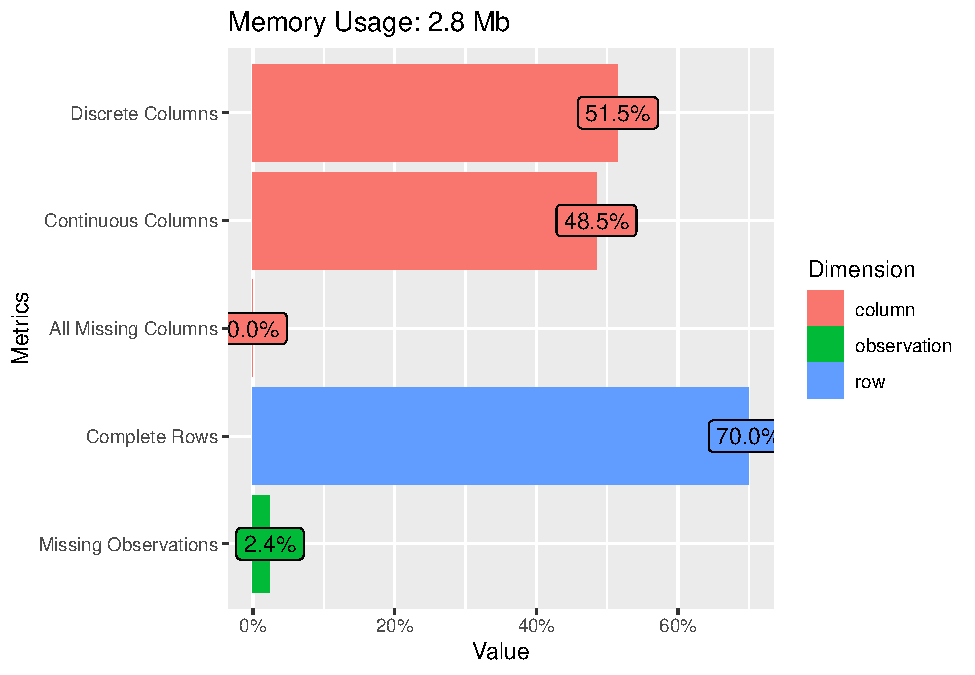
\includegraphics{_main_files/figure-latex/explore_dt_0-1.pdf}

\begin{Shaded}
\begin{Highlighting}[]
\CommentTok{\# plots percentages missing across variables}
\FunctionTok{plot\_missing}\NormalTok{(data\_nba, }\AttributeTok{missing\_only =} \ConstantTok{TRUE}\NormalTok{)}
\end{Highlighting}
\end{Shaded}

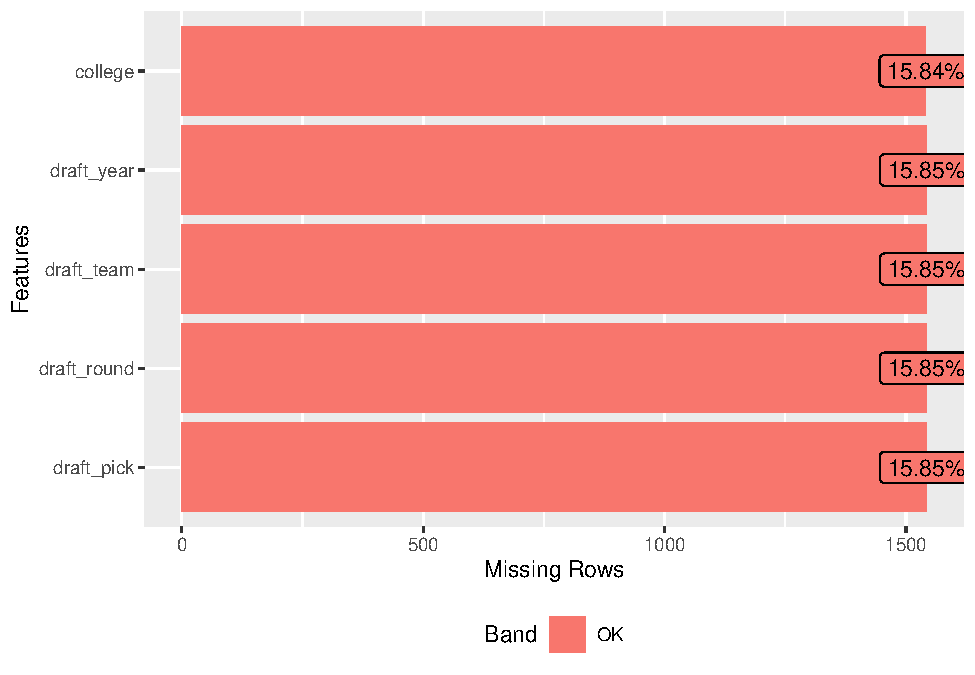
\includegraphics{_main_files/figure-latex/explore_dt_0-2.pdf}

\begin{Shaded}
\begin{Highlighting}[]
\CommentTok{\# plots frequencies across variables (here for a selected subset)}
\NormalTok{data\_nba }\SpecialCharTok{\%\textgreater{}\%} 
  \FunctionTok{select}\NormalTok{(shoots, }\FunctionTok{contains}\NormalTok{(}\StringTok{"position"}\NormalTok{)) }\SpecialCharTok{\%\textgreater{}\%} 
  \FunctionTok{plot\_bar}\NormalTok{()}
\end{Highlighting}
\end{Shaded}

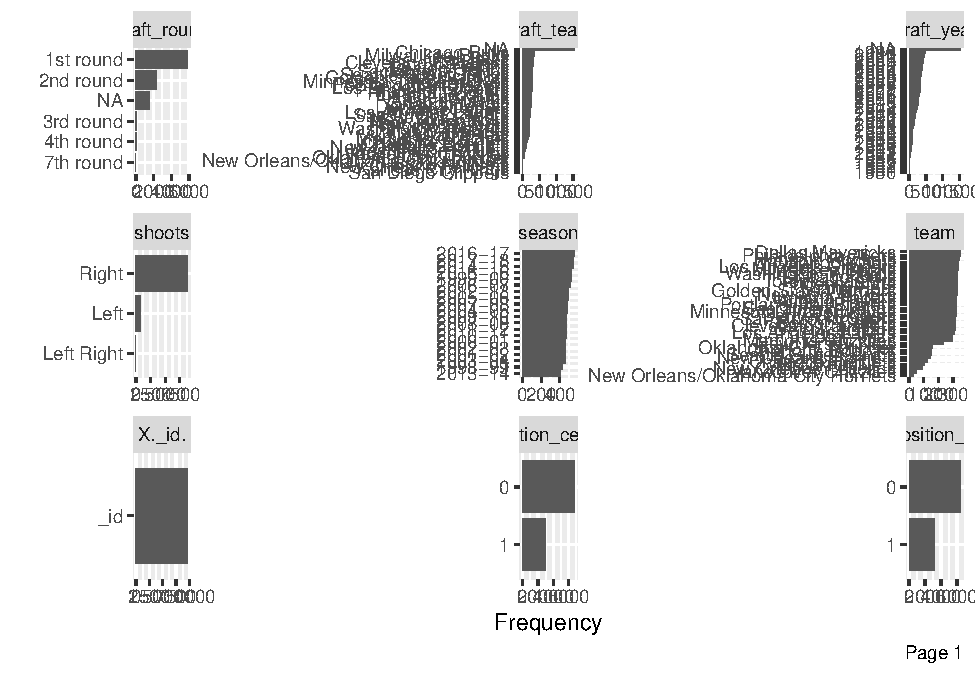
\includegraphics{_main_files/figure-latex/explore_dt_0-3.pdf}

Now, let us try \texttt{gtSummary} for summary tables. A summary table is always a useful start, once you have identified the variables you are interested in.

Let us assume we are interested in \texttt{age}, \texttt{seasons\_played}, \texttt{shoots} (shooting hand), \texttt{career\_PTS} (career points), \texttt{salary} and \texttt{position}.

\begin{Shaded}
\begin{Highlighting}[]
\FunctionTok{library}\NormalTok{(gtsummary)}

\NormalTok{data\_nba }\SpecialCharTok{\%\textgreater{}\%} 
  \FunctionTok{select}\NormalTok{(age, seasons\_played, shoots, career\_PTS, salary, }\FunctionTok{contains}\NormalTok{(}\StringTok{"position"}\NormalTok{)) }\SpecialCharTok{\%\textgreater{}\%}
         \FunctionTok{tbl\_summary}\NormalTok{(}
           \AttributeTok{statistic =} \FunctionTok{all\_continuous}\NormalTok{() }\SpecialCharTok{\textasciitilde{}} \FunctionTok{c}\NormalTok{(}\StringTok{"\{mean\} (\{min\}, \{max\})"}\NormalTok{)) }
\end{Highlighting}
\end{Shaded}

\begin{tabular}{l|c}
\hline
**Characteristic** & **N = 9,728**\\
\hline
age & 27.0 (18.0, 42.0)\\
\hline
seasons\_played & 9 (1, 21)\\
\hline
shoots & \\
\hline
Left & 856 (8.8\%)\\
\hline
Left Right & 7 (<0.1\%)\\
\hline
Right & 8,865 (91\%)\\
\hline
career\_PTS & 8.9 (0.0, 30.1)\\
\hline
salary & 4,072,633 (2,706, 34,682,550)\\
\hline
position\_center & 2,986 (31\%)\\
\hline
position\_sf & 3,222 (33\%)\\
\hline
position\_pf & 3,501 (36\%)\\
\hline
position\_sg & 3,447 (35\%)\\
\hline
position\_pg & 2,489 (26\%)\\
\hline
\end{tabular}

To explore correlations between all numeric variables in the data set, we can inspect the \emph{correlation matrix} or plot it.

\begin{Shaded}
\begin{Highlighting}[]
\CommentTok{\# selct only numeric variables and remove missing values}
\NormalTok{data\_nba\_numeric }\OtherTok{\textless{}{-}}\NormalTok{ data\_nba }\SpecialCharTok{\%\textgreater{}\%}
  \FunctionTok{select}\NormalTok{(}\FunctionTok{where}\NormalTok{(is.numeric)) }\SpecialCharTok{\%\textgreater{}\%}
  \FunctionTok{na.omit}\NormalTok{()}

\CommentTok{\# as a matrix using the corrr package}
\FunctionTok{library}\NormalTok{(}\StringTok{"corrr"}\NormalTok{)}

\NormalTok{corrmatrix }\OtherTok{\textless{}{-}}\NormalTok{ data\_nba\_numeric }\SpecialCharTok{\%\textgreater{}\%}
  \FunctionTok{correlate}\NormalTok{() }\SpecialCharTok{\%\textgreater{}\%} \CommentTok{\# create correlation data frame (cor\_df)}
  \FunctionTok{rearrange}\NormalTok{() }\SpecialCharTok{\%\textgreater{}\%} \CommentTok{\# rearrange by correlations}
  \FunctionTok{shave}\NormalTok{() }\CommentTok{\# remove the upper triangle of the matrix}

\FunctionTok{fashion}\NormalTok{(corrmatrix) }\CommentTok{\# gives a clean display of the matrix}
\end{Highlighting}
\end{Shaded}

\begin{verbatim}
##               term career_AST position_pg career_PTS career_G career_WS
## 1       career_AST                                                     
## 2      position_pg        .61                                          
## 3       career_PTS        .61         .08                              
## 4         career_G        .47         .04        .65                   
## 5        career_WS        .52        -.01        .76      .83          
## 6   seasons_played        .33         .04        .48      .79       .61
## 7      position_sg        .19         .22        .12      .09       .01
## 8           salary        .35        -.04        .60      .48       .59
## 9              age        .18         .03        .18      .49       .36
## 10     position_sf       -.08        -.33        .12      .13       .07
## 11      season_end        .01         .01        .04     -.17      -.09
## 12    season_start        .01         .01        .04     -.17      -.09
## 13          height       -.31        -.46       -.01     -.02      -.00
## 14     position_pf       -.29        -.44        .01      .11       .12
## 15 position_center       -.36        -.39       -.10      .04       .08
## 16          weight       -.49        -.66       -.06     -.03       .05
##    seasons_played position_sg salary  age position_sf season_end season_start
## 1                                                                            
## 2                                                                            
## 3                                                                            
## 4                                                                            
## 5                                                                            
## 6                                                                            
## 7             .09                                                            
## 8             .41        -.03                                                
## 9             .26         .03    .25                                         
## 10            .12         .18    .03  .03                                    
## 11            .00         .02    .16 -.07        -.04                        
## 12            .00         .02    .16 -.07        -.04       1.00             
## 13           -.03        -.03    .03 -.04         .30        .02          .02
## 14            .12        -.46    .09  .03         .04       -.00         -.00
## 15            .07        -.49    .10  .04        -.37       -.06         -.06
## 16            .04        -.43    .12 -.07        -.01        .04          .04
##    height position_pf position_center weight
## 1                                           
## 2                                           
## 3                                           
## 4                                           
## 5                                           
## 6                                           
## 7                                           
## 8                                           
## 9                                           
## 10                                          
## 11                                          
## 12                                          
## 13                                          
## 14    .15                                   
## 15    .12         .33                       
## 16    .41         .45             .66
\end{verbatim}

\begin{Shaded}
\begin{Highlighting}[]
\CommentTok{\# or plot it using a ggplot approach}
\FunctionTok{library}\NormalTok{(}\StringTok{"ggcorrplot"}\NormalTok{)}

\NormalTok{corrmatrix }\OtherTok{\textless{}{-}} \FunctionTok{round}\NormalTok{(}\FunctionTok{cor}\NormalTok{(data\_nba\_numeric), }\DecValTok{1}\NormalTok{) }\CommentTok{\# create correlation matrix}

\FunctionTok{ggcorrplot}\NormalTok{(corrmatrix,}
           \AttributeTok{method =} \StringTok{"circle"}\NormalTok{,}
           \AttributeTok{type=}\StringTok{"lower"}\NormalTok{) }\CommentTok{\# plots the matrix}
\end{Highlighting}
\end{Shaded}

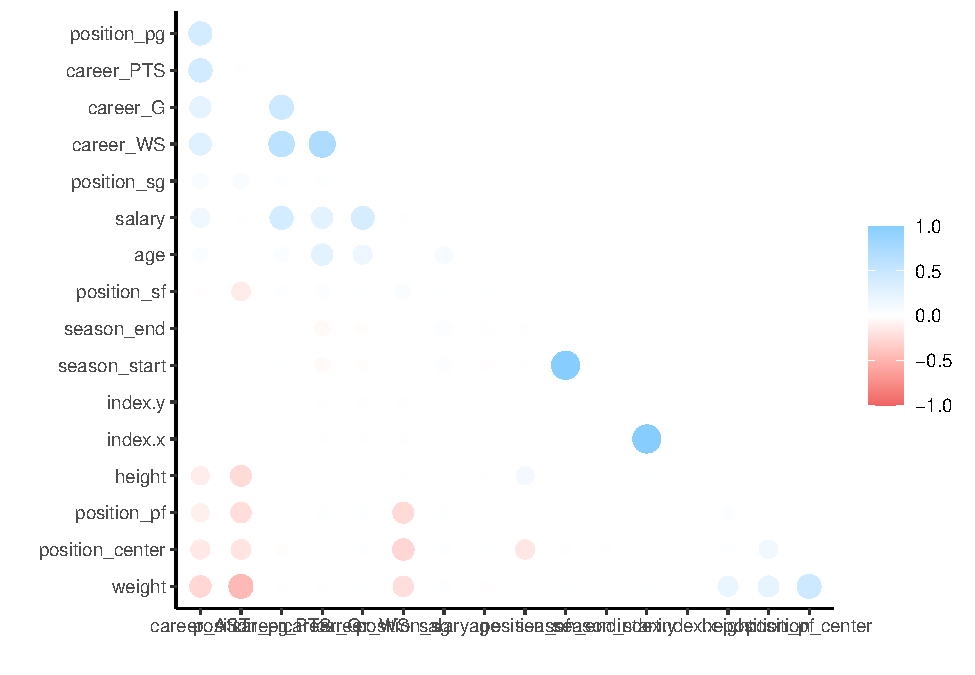
\includegraphics{_main_files/figure-latex/explore_dt_2-1.pdf}

This is interesting. For example, it seems that the weight is strongly correlated with the position a player occupies. Centers are heavy, point guards are light weights. We also see that most performance metrics (\texttt{career\_*}) are correlated with each other and also with salary. Good players seem to be good in many things, and good players seem to be paid more.

\hypertarget{explore-individual-variables}{%
\section{Explore individual variables}\label{explore-individual-variables}}

Now that we have a feeling for the whole data set, we want to explore individual variables. To keep it focused, we will follow up on the question of whether players that perform better are also paid more, for now limiting ourselves to the relationship between the average points per game and the received salary. We will also explore if this relationship depends on the position a player occupies.

Why might the position be relevant for this? We can expect that the justification for the salary differs by the occupied position, i.e.~the role a player fills for the team. To explore this we will limit ourselves to two positions for now, point guards and centers. Point guards are really good passers. Their salary may thus depend more on enabling others to score and not so much on their own point average. Centers on the other hand will mostly be on the receiving end, transforming passes into points. For them their salary may more strongly depend on the actual points they are able to score. This clearly still is an oversimplification of how basketball works but may be a first avenue to approach the relationship between salary and point average.

Let us first build a new variable that discerns between centers, point guards and all other positions and that is easier to work with when comparing the distributions. As we have seen above, there are players that play several positions. We should first check if there are centers who are also point guards, and vice versa. For simple cross tabulations, we can use the base R function \texttt{table()}.

\begin{Shaded}
\begin{Highlighting}[]
\FunctionTok{table}\NormalTok{(data\_nba}\SpecialCharTok{$}\NormalTok{position\_center, data\_nba}\SpecialCharTok{$}\NormalTok{position\_pg)}
\end{Highlighting}
\end{Shaded}

\begin{verbatim}
##    
##        0    1
##   0 4253 2489
##   1 2986    0
\end{verbatim}

We can see that there are \(0\) observations for which both variables equal \(1\). This saves us some headaches and we can construct the new variable in a straightforward way.

\begin{Shaded}
\begin{Highlighting}[]
\NormalTok{data\_nba }\OtherTok{\textless{}{-}}\NormalTok{ data\_nba }\SpecialCharTok{\%\textgreater{}\%} 
  \FunctionTok{mutate}\NormalTok{(}\AttributeTok{role =} \FunctionTok{case\_when}\NormalTok{(}
\NormalTok{    position\_pg }\SpecialCharTok{==} \DecValTok{1} \SpecialCharTok{\textasciitilde{}} \StringTok{"pg"}\NormalTok{,}
\NormalTok{    position\_center }\SpecialCharTok{==} \DecValTok{1} \SpecialCharTok{\textasciitilde{}} \StringTok{"center"}\NormalTok{,}
    \ConstantTok{TRUE} \SpecialCharTok{\textasciitilde{}} \StringTok{"other"}
\NormalTok{  ))}
\end{Highlighting}
\end{Shaded}

Let us start with the \texttt{salary} variable. There are several possible approaches to exploring the distributions of our variables of interest. We could for one use functions like \texttt{skim()} or \texttt{summary()}, but we can also construct a table with some summary statistics of interest ourselves using \texttt{summarise()}.

\begin{Shaded}
\begin{Highlighting}[]
\NormalTok{data\_nba }\SpecialCharTok{\%\textgreater{}\%} 
  \FunctionTok{summarise}\NormalTok{(}\AttributeTok{min =} \FunctionTok{min}\NormalTok{(salary),}
            \AttributeTok{p25 =} \FunctionTok{quantile}\NormalTok{(salary, }\AttributeTok{probs =} \FloatTok{0.25}\NormalTok{),}
            \AttributeTok{median =} \FunctionTok{median}\NormalTok{(salary),}
            \AttributeTok{mean =} \FunctionTok{mean}\NormalTok{(salary),}
            \AttributeTok{p75 =} \FunctionTok{quantile}\NormalTok{(salary, }\AttributeTok{probs =} \FloatTok{0.75}\NormalTok{),}
            \AttributeTok{max =} \FunctionTok{max}\NormalTok{(salary)}
\NormalTok{            )}
\end{Highlighting}
\end{Shaded}

\begin{verbatim}
## # A tibble: 1 x 6
##     min    p25  median     mean     p75      max
##   <dbl>  <dbl>   <dbl>    <dbl>   <dbl>    <dbl>
## 1  2706 947907 2240000 4072633. 5408700 34682550
\end{verbatim}

This already gives us some indication on the distribution of the variable but we may ease the interpretation using plots.

\begin{Shaded}
\begin{Highlighting}[]
\CommentTok{\# using a boxplot}
\NormalTok{data\_nba }\SpecialCharTok{\%\textgreater{}\%}
  \FunctionTok{ggplot}\NormalTok{(}\FunctionTok{aes}\NormalTok{(}\AttributeTok{x =}\NormalTok{ salary)) }\SpecialCharTok{+}
  \FunctionTok{geom\_boxplot}\NormalTok{()}
\end{Highlighting}
\end{Shaded}

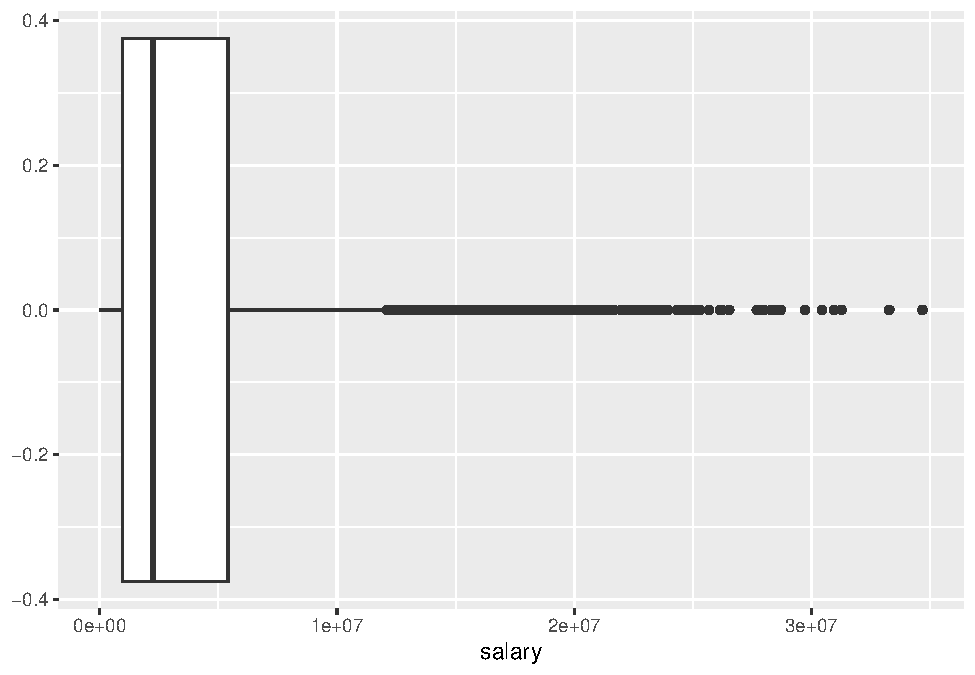
\includegraphics{_main_files/figure-latex/plot_distribution_salary-1.pdf}

\begin{Shaded}
\begin{Highlighting}[]
\CommentTok{\# using a histogram}
\NormalTok{data\_nba }\SpecialCharTok{\%\textgreater{}\%}
  \FunctionTok{ggplot}\NormalTok{(}\FunctionTok{aes}\NormalTok{(}\AttributeTok{x =}\NormalTok{ salary)) }\SpecialCharTok{+}
  \FunctionTok{geom\_histogram}\NormalTok{(}\AttributeTok{bins =} \DecValTok{50}\NormalTok{)}
\end{Highlighting}
\end{Shaded}

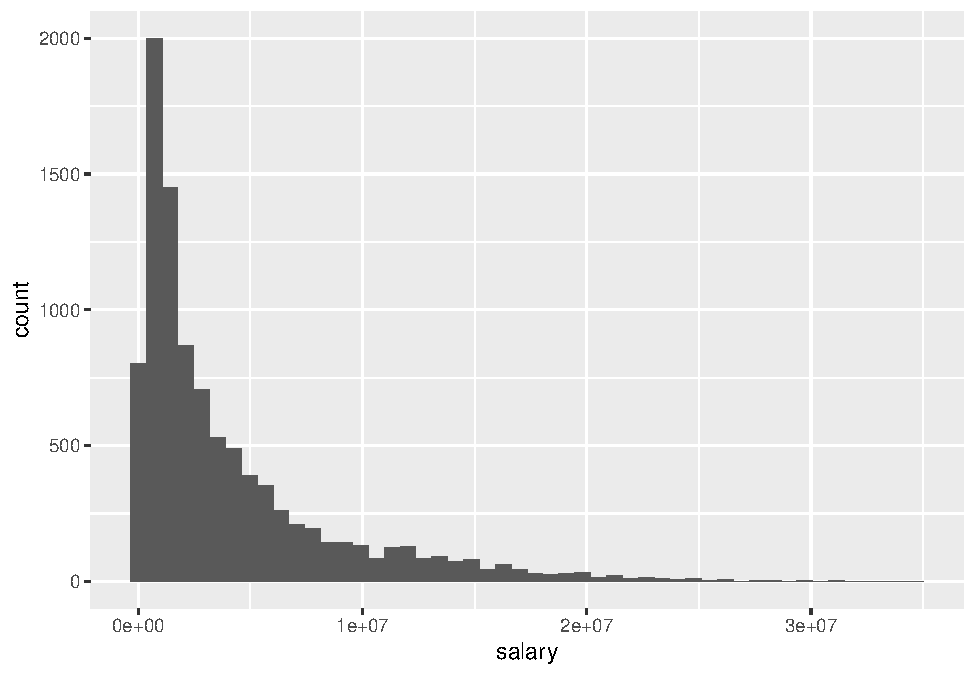
\includegraphics{_main_files/figure-latex/plot_distribution_salary-2.pdf}

\begin{Shaded}
\begin{Highlighting}[]
\CommentTok{\# using a density plot}
\NormalTok{data\_nba }\SpecialCharTok{\%\textgreater{}\%}
  \FunctionTok{ggplot}\NormalTok{(}\FunctionTok{aes}\NormalTok{(}\AttributeTok{x =}\NormalTok{ salary)) }\SpecialCharTok{+}
  \FunctionTok{geom\_density}\NormalTok{()}
\end{Highlighting}
\end{Shaded}

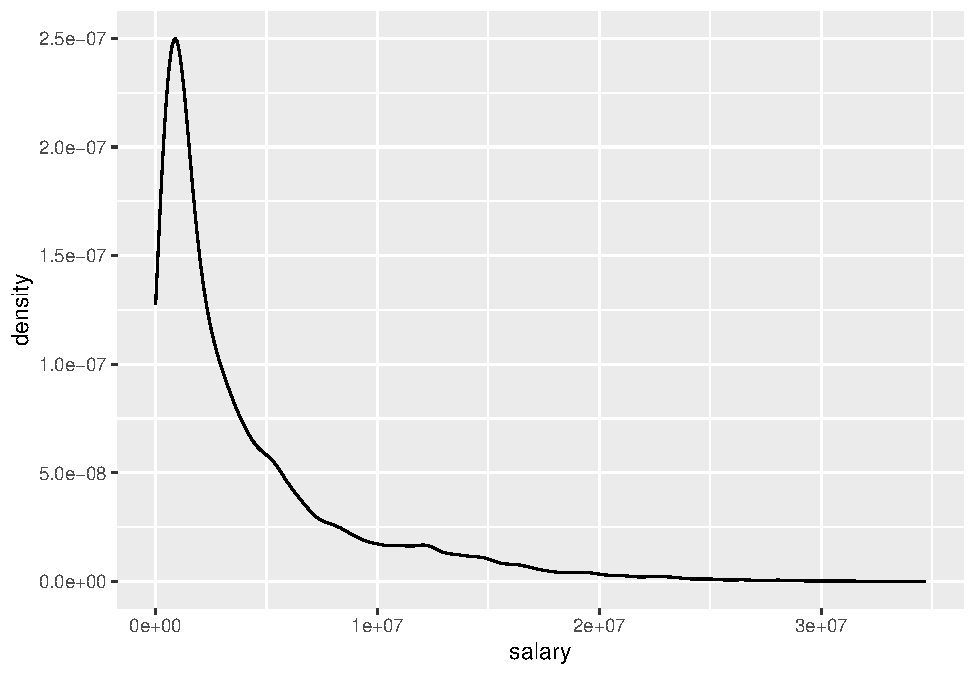
\includegraphics{_main_files/figure-latex/plot_distribution_salary-3.pdf}

The different approaches to visualizing the distribution for \texttt{salary} basically show us the same thing, the distribution is heavily skewed as we see many players with comparably modest salaries and increasingly few with very high compensations. We should keep this in mind when we turn to building a regression model.

We can also compute and visualize the distribution by the role a player fills. Using \texttt{summarise()} with \texttt{group\_by()} enables us to get the same measurements as above, but separately for each category of \texttt{role}.

\begin{Shaded}
\begin{Highlighting}[]
\NormalTok{data\_nba }\SpecialCharTok{\%\textgreater{}\%} 
  \FunctionTok{group\_by}\NormalTok{(role) }\SpecialCharTok{\%\textgreater{}\%} 
  \FunctionTok{summarise}\NormalTok{(}\AttributeTok{min =} \FunctionTok{min}\NormalTok{(salary),}
            \AttributeTok{p25 =} \FunctionTok{quantile}\NormalTok{(salary, }\AttributeTok{probs =} \FloatTok{0.25}\NormalTok{),}
            \AttributeTok{median =} \FunctionTok{median}\NormalTok{(salary),}
            \AttributeTok{mean =} \FunctionTok{mean}\NormalTok{(salary),}
            \AttributeTok{p75 =} \FunctionTok{quantile}\NormalTok{(salary, }\AttributeTok{probs =} \FloatTok{0.75}\NormalTok{),}
            \AttributeTok{max =} \FunctionTok{max}\NormalTok{(salary)}
\NormalTok{            )}
\end{Highlighting}
\end{Shaded}

\begin{verbatim}
## # A tibble: 3 x 7
##   role     min     p25  median     mean     p75      max
##   <chr>  <dbl>   <dbl>   <dbl>    <dbl>   <dbl>    <dbl>
## 1 center  4529 1115340 2880000 4770707. 6400000 28000000
## 2 other   2706  863640 2000000 3757860. 5000000 33285709
## 3 pg      2853  895248 2100000 3773028. 5000000 34682550
\end{verbatim}

For plotting by role, let us limit ourselves to boxplots.

\begin{Shaded}
\begin{Highlighting}[]
\NormalTok{data\_nba }\SpecialCharTok{\%\textgreater{}\%}
  \FunctionTok{ggplot}\NormalTok{(}\FunctionTok{aes}\NormalTok{(}\AttributeTok{x =}\NormalTok{ salary, }\AttributeTok{colour =}\NormalTok{ role)) }\SpecialCharTok{+}
  \FunctionTok{geom\_boxplot}\NormalTok{()}
\end{Highlighting}
\end{Shaded}

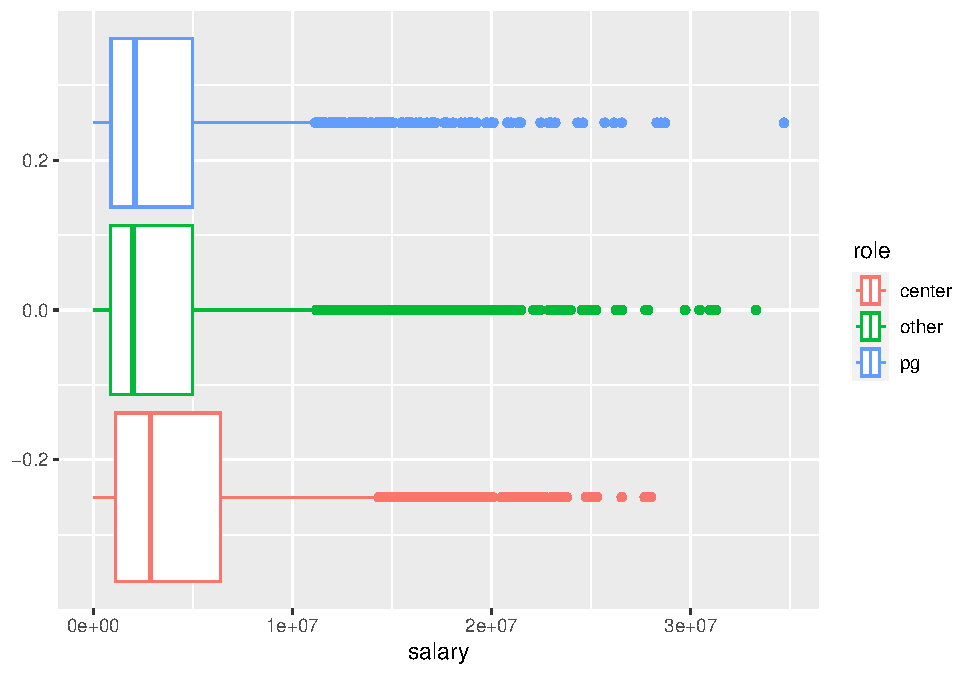
\includegraphics{_main_files/figure-latex/plot_distribution_salary_role-1.pdf}

We can see, that while point guards barely differ from their peers, centers do. The average salary for centers is higher compared to all other roles. At the same time while many of them reach very high salaries, the top earner spots are reserved for other roles. The highest earning point guard makes almost \(6,700,000\$\) more compared to the highest earning center; a substantial difference. As the boxplot indicates, the players with such extreme salaries are also in the extreme minority so we should not over interpret this finding. Still, the puzzle seems to be more complex than we thought.

Let us turn to \texttt{career\_PTS} now and repeat the analysis from above.

\begin{Shaded}
\begin{Highlighting}[]
\NormalTok{data\_nba }\SpecialCharTok{\%\textgreater{}\%} 
  \FunctionTok{summarise}\NormalTok{(}\AttributeTok{min =} \FunctionTok{min}\NormalTok{(career\_PTS),}
            \AttributeTok{p25 =} \FunctionTok{quantile}\NormalTok{(career\_PTS, }\AttributeTok{probs =} \FloatTok{0.25}\NormalTok{),}
            \AttributeTok{median =} \FunctionTok{median}\NormalTok{(career\_PTS),}
            \AttributeTok{mean =} \FunctionTok{mean}\NormalTok{(career\_PTS),}
            \AttributeTok{p75 =} \FunctionTok{quantile}\NormalTok{(career\_PTS, }\AttributeTok{probs =} \FloatTok{0.75}\NormalTok{),}
            \AttributeTok{max =} \FunctionTok{max}\NormalTok{(career\_PTS)}
\NormalTok{            )}
\end{Highlighting}
\end{Shaded}

\begin{verbatim}
## # A tibble: 1 x 6
##     min   p25 median  mean   p75   max
##   <dbl> <dbl>  <dbl> <dbl> <dbl> <dbl>
## 1     0   5.1      8  8.91    12  30.1
\end{verbatim}

\begin{Shaded}
\begin{Highlighting}[]
\NormalTok{data\_nba }\SpecialCharTok{\%\textgreater{}\%}
  \FunctionTok{ggplot}\NormalTok{(}\FunctionTok{aes}\NormalTok{(}\AttributeTok{x =}\NormalTok{ career\_PTS)) }\SpecialCharTok{+}
  \FunctionTok{geom\_boxplot}\NormalTok{()}
\end{Highlighting}
\end{Shaded}

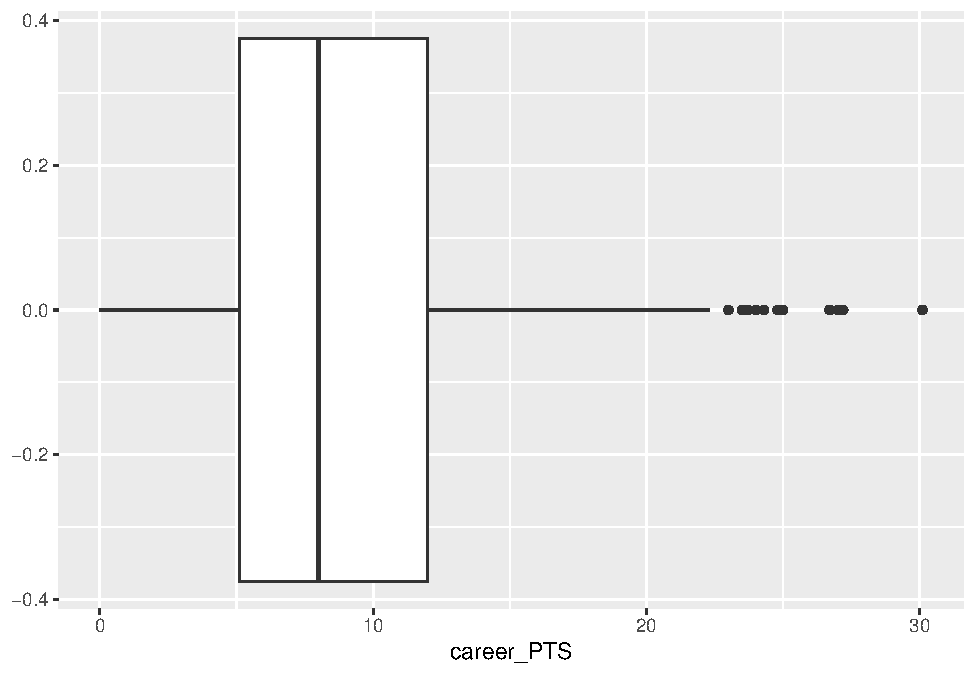
\includegraphics{_main_files/figure-latex/summarise_distribution_points-1.pdf}

\begin{Shaded}
\begin{Highlighting}[]
\NormalTok{data\_nba }\SpecialCharTok{\%\textgreater{}\%}
  \FunctionTok{ggplot}\NormalTok{(}\FunctionTok{aes}\NormalTok{(}\AttributeTok{x =}\NormalTok{ career\_PTS)) }\SpecialCharTok{+}
  \FunctionTok{geom\_histogram}\NormalTok{(}\AttributeTok{bins =} \DecValTok{50}\NormalTok{)}
\end{Highlighting}
\end{Shaded}

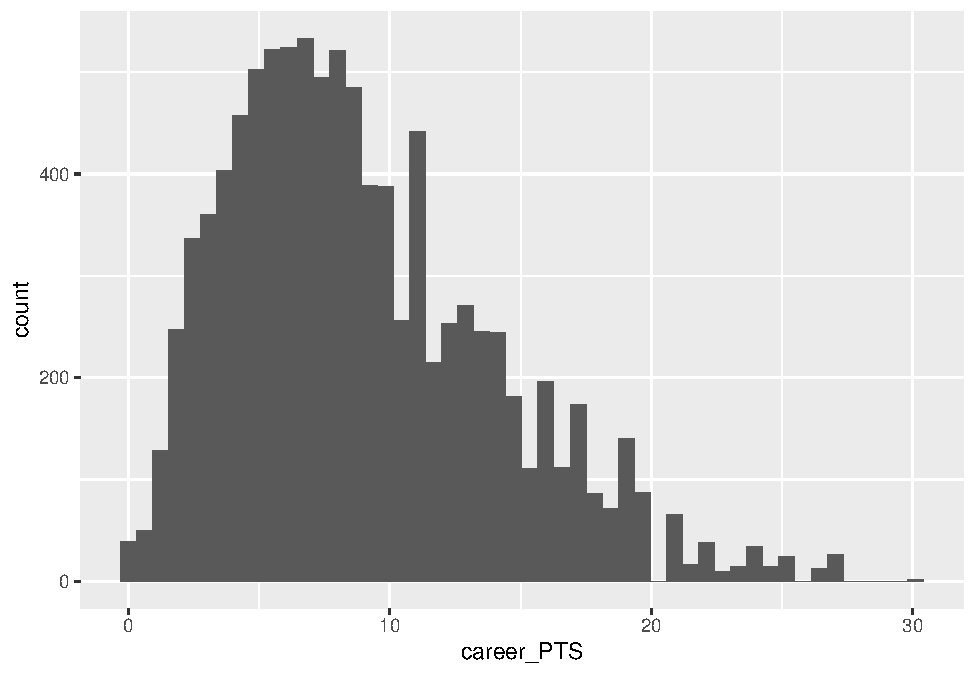
\includegraphics{_main_files/figure-latex/summarise_distribution_points-2.pdf}

While the distribution of average career points is also somewhat skewed, it is way less so compared to \texttt{salary}.

We should also look at \texttt{career\_PTS} by role.

\begin{Shaded}
\begin{Highlighting}[]
\NormalTok{data\_nba }\SpecialCharTok{\%\textgreater{}\%} 
  \FunctionTok{group\_by}\NormalTok{(role) }\SpecialCharTok{\%\textgreater{}\%} 
  \FunctionTok{summarise}\NormalTok{(}\AttributeTok{min =} \FunctionTok{min}\NormalTok{(career\_PTS),}
            \AttributeTok{p25 =} \FunctionTok{quantile}\NormalTok{(career\_PTS, }\AttributeTok{probs =} \FloatTok{0.25}\NormalTok{),}
            \AttributeTok{median =} \FunctionTok{median}\NormalTok{(career\_PTS),}
            \AttributeTok{mean =} \FunctionTok{mean}\NormalTok{(career\_PTS),}
            \AttributeTok{p75 =} \FunctionTok{quantile}\NormalTok{(career\_PTS, }\AttributeTok{probs =} \FloatTok{0.75}\NormalTok{),}
            \AttributeTok{max =} \FunctionTok{max}\NormalTok{(career\_PTS)}
\NormalTok{            )}
\end{Highlighting}
\end{Shaded}

\begin{verbatim}
## # A tibble: 3 x 7
##   role     min   p25 median  mean   p75   max
##   <chr>  <dbl> <dbl>  <dbl> <dbl> <dbl> <dbl>
## 1 center     0   4.5    7    8.17  11.2  24.3
## 2 other      0   5.2    8.2  9.04  12    30.1
## 3 pg         0   6.3    8.9  9.57  12.6  26.7
\end{verbatim}

\begin{Shaded}
\begin{Highlighting}[]
\NormalTok{data\_nba }\SpecialCharTok{\%\textgreater{}\%}
  \FunctionTok{ggplot}\NormalTok{(}\FunctionTok{aes}\NormalTok{(}\AttributeTok{x =}\NormalTok{ career\_PTS, }\AttributeTok{colour =}\NormalTok{ role)) }\SpecialCharTok{+}
  \FunctionTok{geom\_boxplot}\NormalTok{()}
\end{Highlighting}
\end{Shaded}

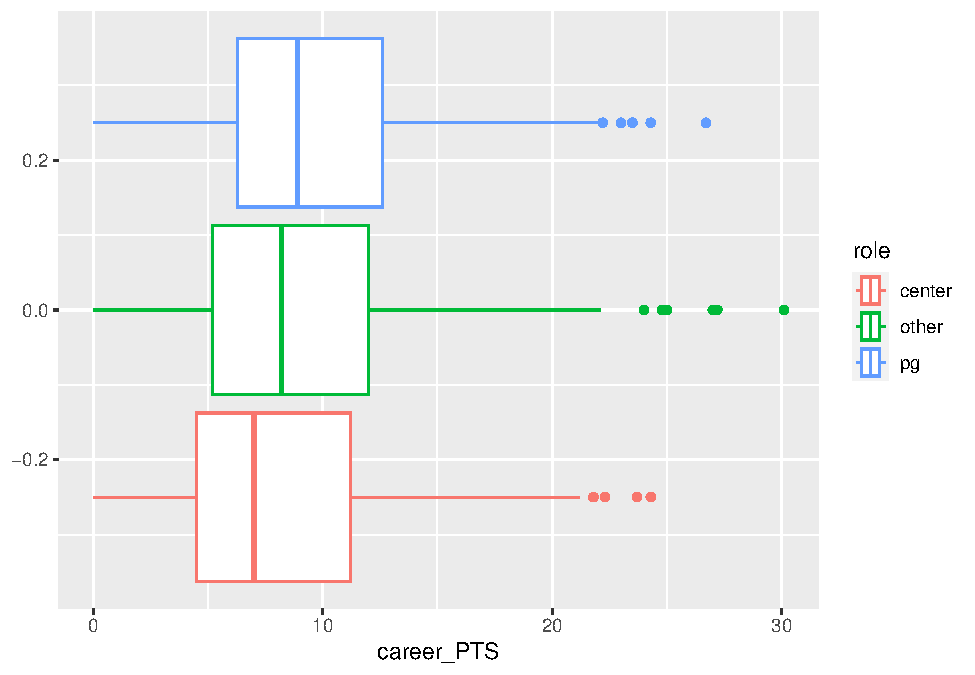
\includegraphics{_main_files/figure-latex/summarise_distribution_points_role-1.pdf}

Centers actually make less points on average compared to all other roles and point guards score the highest on average. That is an interesting puzzle to explore. It seems that point guards are paid a little less even though they make a few more points on average. What does this tell us? We can not be sure yet, but it seems that the relationship between points and salary gets translated differently based on the role a player occupies.

Let us now explore this relationship between the two variables, which will be central to our analysis from now on. We can use a scatter plot to inspect the shared distribution of both variables. We also added a line describing the relationship. This actually is a regression line and we will talk about it in detail \protect\hyperlink{lin-t-1}{later}, for now let us just accept that the direction of the line tells us how both variables are related.

\begin{Shaded}
\begin{Highlighting}[]
\NormalTok{data\_nba }\SpecialCharTok{\%\textgreater{}\%} 
  \FunctionTok{ggplot}\NormalTok{(}\FunctionTok{aes}\NormalTok{(}\AttributeTok{y =}\NormalTok{ salary, }\AttributeTok{x =}\NormalTok{ career\_PTS)) }\SpecialCharTok{+}
  \FunctionTok{geom\_point}\NormalTok{() }\SpecialCharTok{+}
  \FunctionTok{geom\_smooth}\NormalTok{(}\AttributeTok{method =} \StringTok{"lm"}\NormalTok{)}
\end{Highlighting}
\end{Shaded}

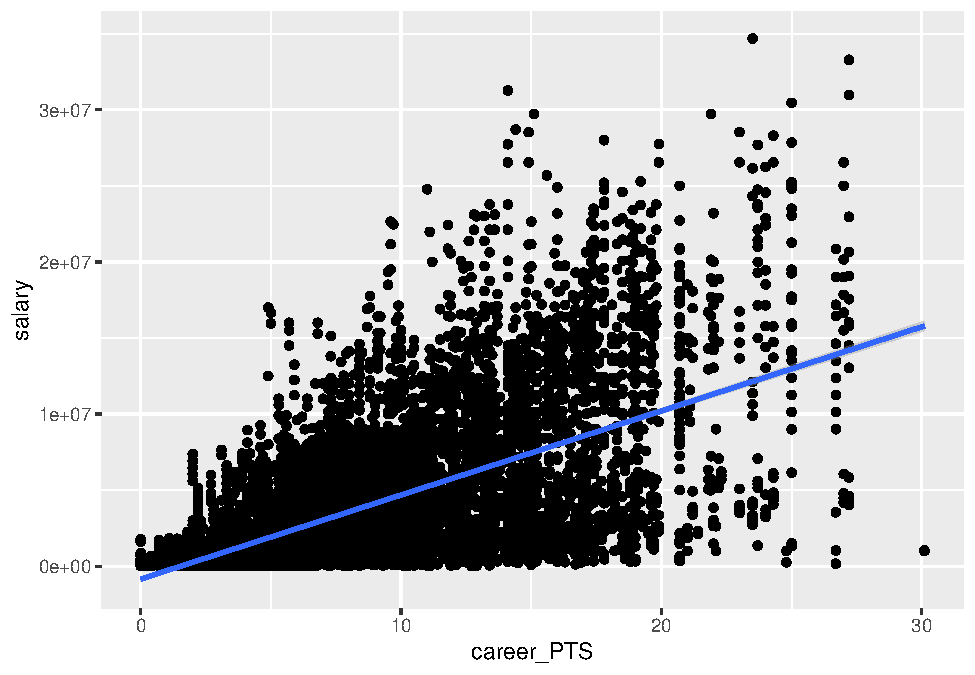
\includegraphics{_main_files/figure-latex/salary_points_scatter-1.pdf}

We can see that there is a positive relationship between the average score and the earned salary. The more points a player scores the more he earns, on average.

We can build the same plot by \texttt{role}.

\begin{Shaded}
\begin{Highlighting}[]
\NormalTok{data\_nba }\SpecialCharTok{\%\textgreater{}\%} 
  \FunctionTok{ggplot}\NormalTok{(}\FunctionTok{aes}\NormalTok{(}\AttributeTok{y =}\NormalTok{ salary, }\AttributeTok{x =}\NormalTok{ career\_PTS, }\AttributeTok{colour =}\NormalTok{ role)) }\SpecialCharTok{+}
  \FunctionTok{geom\_point}\NormalTok{(}\AttributeTok{alpha =} \FloatTok{0.25}\NormalTok{) }\SpecialCharTok{+}
  \FunctionTok{geom\_smooth}\NormalTok{(}\AttributeTok{method =} \StringTok{"lm"}\NormalTok{)}
\end{Highlighting}
\end{Shaded}

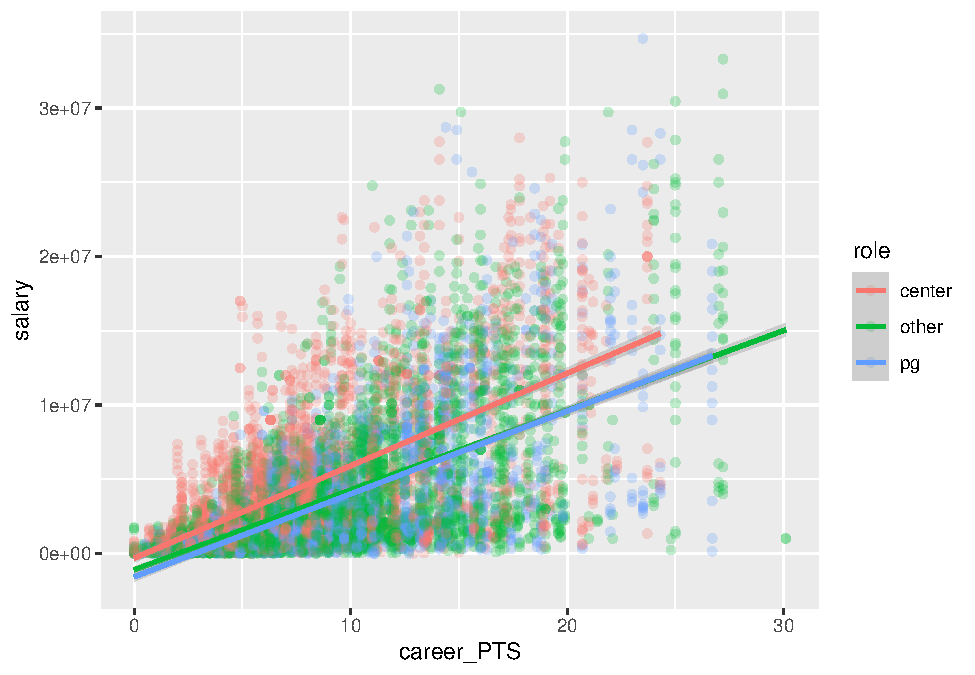
\includegraphics{_main_files/figure-latex/salary_points_role_scatter-1.pdf}

Let's reflect a moment what we can learn from all this.

First, there seems to be a somewhat linear relationship between how many points a player scores and how much they are paid. This also holds true for point guards just as much as for non-point guards. However, the average salary for point guards is lower in comparison. We also learn that the link between salary and points is stronger for centers as the red line is somewhat steeper. They seem to be paid more, the more they score.

\hypertarget{moving-on}{%
\section{Moving on}\label{moving-on}}

We have now explored our data and gained a better understanding of the variables of interest. We also have identified an interesting puzzle to explre further, and we will pick up on this over the seminar. In \protect\hyperlink{dags-1}{week 4}, we will construct a theoretical model that tries to explain the relationship between points and salary and in \protect\hyperlink{lin-a}{week 8} we will then compute a linear regression model that will hopefully shed some more light on our puzzle. Linear regression is all about further exploring the relationship between two or more variables, one outcome (often called \texttt{y}) and one or multiple independent variables (often called \texttt{x}). Independent variables have many names. They are sometimes called ``covariates''; ``predictors''; ``exposure'', depending on the context.

There are a number of cool things that regression can do for us that simple EDA cannot:

\begin{enumerate}
\def\labelenumi{\arabic{enumi})}
\item
  It can model the relationship between two variables while considering simultaneously the potential influence of other factors. Imagine we are interested in the effect of points per game on salary regardless of position, season, team or other independent variables. With regression we can estimate how much more a player would earn every season if he scored 10 more points a game (regardless of other factors as for example the position he plays).
\item
  It can assess what explains the effect of one variable on another (i.e.~mediation). Maybe we find that point guards earn less and we want to know why. Is it because they score less? Is it because they play less time on average?
\item
  It can be used to predict salaries for players for whom we don't know the salary or even for hypothetical players. We could also look at the performance trend of players and predict whether they earn more next season or not.
\end{enumerate}

We will address all these applications over the course of the seminar.

\hypertarget{further-resources}{%
\section{Further resources}\label{further-resources}}

\begin{itemize}
\tightlist
\item
  \href{https://tuos-bio-data-skills.github.io/intro-eda-book/index.html}{Exploratory Data Analysis with R}, a book that covers the basics of data visualization, manipulation, and analysis using R and the tidyverse package.
\item
  \href{https://www.pluralsight.com/guides/exploratory-data-analysis-in-r}{Exploratory Data Analysis in R with Tidyverse}, a guide that shows how to use the tidyverse package to perform common EDA tasks such as importing, cleaning, summarizing, and plotting data.
\item
  \href{https://r4ds.had.co.nz/data-visualisation.html}{Data Visualization with ggplot2}, a chapter from the book R for Data Science that explains how to create and customize different types of plots using the ggplot2 package.
\item
  \href{https://r4ds.had.co.nz/transform.html}{Data Transformation with dplyr}, another chapter from the book R for Data Science that demonstrates how to use the dplyr package to manipulate data frames, filter rows, select columns, create new variables, and more.
\item
  \href{https://bookdown.org/rdpeng/exdata/}{Exploratory Data Analysis with R - Bookdown}
\item
  \href{https://www.statology.org/exploratory-data-analysis-in-r/}{How to Perform Exploratory Data Analysis in R (With Example)}
\end{itemize}

\hypertarget{eda-2}{%
\chapter{Exploratory Data Analysis - Exercise}\label{eda-2}}

This week we will apply the concepts from last week in an exercise where you will conduct an exploratory data analysis on a different data set. To document your work on these exercises, you will use \emph{R Markdown}.

\hypertarget{what-is-r-markdown}{%
\section{What is R Markdown?}\label{what-is-r-markdown}}

R Markdown allows you to combine written text that is easy to format with R Code that is executed when \emph{knitting} or \emph{compiling} the document into the chosen output format. This allows us to describe our research, analyse our data, display results as tables or plots and interpret these, all in one file. In this way we can not only create reports on seminar exercises but also write websites - like the one your are looking at in this very moment -, seminar papers, articles or create presentations.

It is also a great notebook for projects you are working on. More often than not, our work on a specific analysis will span multiple days, weeks or even months and it is often hard to remember what we were thinking the last time we worked on our code.

\begin{quote}
``I am sure I had my reasons for writing this piece of code, but I can not for the life of me remember any of them\ldots{}''

--- Anonymous Coder 2023
\end{quote}

If we use R Markdown to document our work we can add text that explains our reasons, thoughts, ideas and plans at that very moment and pick up our work from there the next time we open the file.

R Markdown allows output to different file formats, including \texttt{html}, \texttt{docx}, \texttt{pptx} and \texttt{pdf}. Note that you need a LaTeX installation to knit to \texttt{pdf}. LaTeX is a typesetting language and used for producing high quality \texttt{pdf} documents. For simple \texttt{pdf} reports or presentations - sidenote: if you bring a \texttt{pptx} to a talk something will most probably go wrong or stop working\ldots{} - you do not really need to know how LaTeX works, you just need an installed distribution. For these purposes the package \texttt{tinytex} gives you all you need and is easy to install from within R. \href{https://bookdown.org/yihui/rmarkdown/installation.html\#installation}{This site} explains how to install it. You can also get an overview of all possible output formats \href{https://rmarkdown.rstudio.com/lesson-9.html}{here}.

\hypertarget{creating-a-r-markdown-file}{%
\section{Creating a R Markdown file}\label{creating-a-r-markdown-file}}

Before you can create and compile R Markdown documents, you first have to install the package by writing \texttt{install.packages("rmarkdown")} in your console.

Creating a new R Markdown file is as straightforward as it can be. In RStudio you can click of \texttt{File\ \textgreater{}\ New\ File\ \textgreater{}\ R\ Markdown...}. In the new window you can set up some basic information on the document - which will be displayed in the output - and chose your desired format. You can basically write R Markdown files in any text editor, just make sure that the file extension is saved as \texttt{.Rmd}. We still recommend using RStudio because it gives you some convenient options that a text editor will not, e.g.~displaying a preview of your document and easy knitting of the final file.

\hypertarget{writing-in-r-markdown}{%
\section{Writing in R Markdown}\label{writing-in-r-markdown}}

\hypertarget{document-components}{%
\subsection{Document components}\label{document-components}}

When you followed the steps above, a new R Markdown file will have been created. It basically consists of two main parts:

\begin{itemize}
\item
  A \texttt{YAML} header - surrounded by three dashes \texttt{-\/-\/-} - where options for the document can be set. The good news is that you do not have to do anything here until you get more profound with using R Markdown. For now it is enough that all the options you set when creating the new file - the title, author, date and format of the output - are present and will be included in your output file.
\item
  A body that contains the actual content of your document. Text is directly written in the body at the location where it is to be displayed in the output. We can use the simple Markdown syntax for formatting using a set of symbols, some of which we will explain below. We can also include R code in so called \texttt{chunks}, specifying if we also want it and/or the results to be displayed or ``just'' to be executed in the background. The code chunks will be executed when we compile the final document and everything that we want to include in the output - e.g.~tables, plots or code examples - will be displayed where it occurs.
\end{itemize}

\hypertarget{formatting}{%
\subsection{Formatting}\label{formatting}}

Here are some of the more common formatting elements you will need when starting out using R Markdown:

\hypertarget{headers}{%
\subsubsection{Headers}\label{headers}}

To include sections in a document we use \texttt{\#} followed by the header we want to be displayed. We can define levels for sections by using multiple \texttt{\#} in this way:

\begin{verbatim}
# Section 1
## Section 1.1
## Section 1.2
### Section 1.2.1
### Section 1.2.2
## Section 1.3
# Section 2
\end{verbatim}

\hypertarget{text}{%
\subsubsection{Text}\label{text}}

We write the text between the section headers at the place where it should be displayed in the final document. We can insert line breaks at any point but these will not be rendered in the output. To include an actual paragraph we will have to include a blank line between between two blocks of text. Two emphasize certain words or phrases, we can wrap them in \texttt{*} for italics or \texttt{**} for bold face.

Consider this Markdown code:

\begin{verbatim}
This is the first paragraph.
This still is the first paragraph.

Here begins the second paragraph.
It includes emphasis, by using *italics* and also **bold face** words.
\end{verbatim}

It is rendered as:

This is the first paragraph. This still is the first paragraph.

Here begins the second paragraph. It includes emphasis, by using \emph{italics} and also \textbf{bold face} words.

\hypertarget{lists}{%
\subsubsection{Lists}\label{lists}}

Unordered lists or bullet points can be inserted by adding a \texttt{-}, \texttt{*} or \texttt{+} at the beginning of a line. To create levels, we have to indent lines using tab stops.

\begin{verbatim}
* Level 1
* Level 1
  * Level 2
    * Level 3
  * Level 2
    * Level 3
* Level 1
\end{verbatim}

The above will be rendered as:

\begin{itemize}
\tightlist
\item
  Level 1
\item
  Level 1

  \begin{itemize}
  \tightlist
  \item
    Level 2

    \begin{itemize}
    \tightlist
    \item
      Level 3
    \end{itemize}
  \item
    Level 2

    \begin{itemize}
    \tightlist
    \item
      Level 3
    \end{itemize}
  \end{itemize}
\item
  Level 1
\end{itemize}

We can also create ordered lists by using numbers followed by a \texttt{.} instead of the \texttt{*} etc.

\begin{verbatim}
1.  Bulletpoint 1
2.  Bulletpoint 2
3.  Bulletpoint 3
\end{verbatim}

\begin{enumerate}
\def\labelenumi{\arabic{enumi}.}
\tightlist
\item
  Bulletpoint 1
\item
  Bulletpoint 2
\item
  Bulletpoint 3
\end{enumerate}

\hypertarget{hyperlinks}{%
\subsubsection{Hyperlinks}\label{hyperlinks}}

Hyperlinks can be included as \texttt{\textless{}url\textgreater{}} or \texttt{{[}text{]}(url)}.

\begin{verbatim}
To include a plain url we can use <https://jaspertjaden.github.io/DataAnalysisR/>.
We can also [link](https://jaspertjaden.github.io/DataAnalysisR/) in this way.
\end{verbatim}

To include a plain url we can use \url{https://jaspertjaden.github.io/DataAnalysisR/}. We can also \href{https://jaspertjaden.github.io/DataAnalysisR/}{link} in this way.

\hypertarget{code-chunks}{%
\subsection{Code chunks}\label{code-chunks}}

Codechunks have to be started and ended with three backticks \texttt{\textasciigrave{}\textasciigrave{}\textasciigrave{}}. After the first set of backticks we also have to include \texttt{\{r\}} to let Markdown know that we want to run the code as R code. The code that is written after this and up to the second set of backticks will be executed when knitting the file.

You can see some examples of this in the newly created R Markdown file if you followed the steps above.

We can also always run the code in a chunk before knitting by clicking on the green arrow in the upper right corner of the chunk. We can also execute individual lines of code by placing our keyboard cursor in the line and pressing \texttt{Shift\ +\ Enter}.

\hypertarget{chunk-options}{%
\subsubsection{Chunk options}\label{chunk-options}}

We can change the way code chunks are handled when knitting by adding one or multiple chunk options between the curly brackets like this: \texttt{\{r\ option=value\}}. If we want to use multiple options they have to be written like this: \texttt{\{r\ option1=value1,\ option2=value2\}}.

There are many options available but most are not needed when starting out. The ones that may be of interest to you are:

\begin{itemize}
\tightlist
\item
  \texttt{\{r\ echo=FALSE\}}: This prevents the code to be displayed in the output while the results will be included. This is useful if you want to show the results of a computation or a plot but do not want the document to be cluttered with the underlying code.
\item
  \texttt{\{r\ include=FALSE\}}: This prevents the code as well as the output from being displayed. The code is still run in the background.
\item
  \texttt{\{r\ eval=FALSE\}}: This prevents the code from being run but displays it. This can be useful if you want to show code examples for illustrative purposes.
\end{itemize}

\hypertarget{further-resources-1}{%
\section{Further resources}\label{further-resources-1}}

\begin{itemize}
\tightlist
\item
  \href{https://rmarkdown.rstudio.com/lesson-1.html}{R Markdown Website by RStudio}: A comprehensive introduction to using R Markdown from within RStudio
\item
  \href{https://bookdown.org/yihui/rmarkdown/}{Yihui Xie, J. J. Allaire, Garrett Grolemund. R Markdown: The Definitive Guide}: An in-depth overview over basically everything R Markdown can do
\item
  \href{https://rstudio.github.io/cheatsheets/rmarkdown.pdf}{R Markdown Cheat Sheet}: A cheat sheet for R Markdown, those are always helpful
\end{itemize}

\hypertarget{eda---exercise}{%
\section{EDA - Exercise}\label{eda---exercise}}

In this and all following exercises, we will work with the \textbf{Boston Housing Data}. The data set contains information on 506 census tracts in the US city of Boston from the 1970 census. It contains information on the median value of owner-occupied homes and additional statistics on houses and socio-demographics for each tract.

This is an overview of all variables included in the data set:

\begin{verbatim}
1. crim - per capita crime rate by town
2. zn - proportion of residential land zoned for lots over 25,000 sq.ft.
3. indus - proportion of non-retail business acres per town.
4. chas - Charles River dummy variable (1 if tract bounds river; 0 otherwise)
5. nox - nitric oxides concentration (parts per 10 million)
6. rm - average number of rooms per dwelling
7. age - proportion of owner-occupied units built prior to 1940
8. dis - weighted distances to five Boston employment centres
9. rad - index of accessibility to radial highways
10. tax - full-value property-tax rate per $10,000
11. ptratio - pupil-teacher ratio by town
12. b - 1000(Bk - 0.63)^2 where Bk is the proportion of blacks by town
13. lstat - % lower status of the population
14. medv - Median value of owner-occupied homes in $1000's
\end{verbatim}

For more information on the data set and its implementation in \texttt{mlbench} please follow this \href{https://search.r-project.org/CRAN/refmans/mlbench/html/BostonHousing.html}{link}.

\begin{enumerate}
\def\labelenumi{\arabic{enumi}.}
\item
  \textbf{Prepare your R Markdown File}: Create a new R Markdown file setting the output format to \texttt{html} or \texttt{pdf} (if you have a LaTeX distribution installed) and setting the title, author and date to appropriate values. Remove the sample text and code chunks taking care to not remove the \texttt{YAML} header. Write all solutions in this file using code chunks as well as text to structure the file (headers) and answer the questions. Do not forget to save the file in the format \texttt{your\_name\_exercise\_1.Rmd}. You will have to turn in this file to the lecturers through Moodle.
\item
  \textbf{Import the dataset}: Import the data set by using the code below. The package \texttt{mlbench} conveniently includes the data set. You have to install the package beforehand by writing: \texttt{install.packages("mlbench")}. You should also load the \texttt{tidyverse} package to ease the further analysis. Not that this code also has to be included in your R Markdown file.
\end{enumerate}

\begin{Shaded}
\begin{Highlighting}[]
\FunctionTok{library}\NormalTok{(mlbench)}
\FunctionTok{library}\NormalTok{(tidyverse)}

\FunctionTok{data}\NormalTok{(BostonHousing)}
\end{Highlighting}
\end{Shaded}

\begin{enumerate}
\def\labelenumi{\arabic{enumi}.}
\setcounter{enumi}{2}
\item
  \textbf{Inspect the dataset}: Use the proper functions to inspect the structure and contents of the data set. How many categorical variables are there? How many numerical variables are there? Are there any missing values?
\item
  \textbf{Summarize categorical variables}: Create a frequency table for the categorical variable \texttt{chas} (Charles River dummy variable).
\item
  \textbf{Summarize numerical variables}: Generate summary statistics for the numerical variables crim (per capita crime rate by town), rm (average number of rooms per dwelling) and dis (weighted distances to five Boston employment centres).
\item
  \textbf{Create new variables}: Create a new variable that groups houses by their proximity to employment centers as indicated in the variable \texttt{dis}. Create the three categories \texttt{Near}, \texttt{Medium} and \texttt{Far} based on the value of \texttt{dis}. Choose appropriate cutoff values based on the summary statistics you computed above. Briefly describe your decision.
\item
  \textbf{Compare distributions}: Compare the distribution of \texttt{ptratio} by the newly created variable \texttt{distance\_group} using boxplots. Briefly interpret the results.
\item
  \textbf{Visualize relationships}: Create scatter plots with an added regression line to explore the relationship between housing prices (\texttt{medv}) and the numeric variables : \texttt{rm}, \texttt{age}, \texttt{dis}, \texttt{lstat}. Briefly interpret the plots.
\item
  \textbf{Correlation analysis}: Calculate correlation coefficients between housing prices (\texttt{medv}), the average number of rooms per dwelling (\texttt{rm}) and the crime rate (\texttt{crim}). Display the correlations as a matrix or as a plot. Interpret the result.
\end{enumerate}

\hypertarget{dags-1}{%
\chapter{DAGs}\label{dags-1}}

\hypertarget{objectives-1}{%
\section{Objectives}\label{objectives-1}}

\begin{itemize}
\tightlist
\item
  Getting to know DAGs
\item
  Understand its implications on achieving unbiased estimates for
  effects of interest
\item
  Building a DAG for the NBA data to model the effect of scored points
  on salary
\end{itemize}

\hypertarget{functions-covered}{%
\section{Functions Covered}\label{functions-covered}}

\begin{itemize}
\tightlist
\item
  \texttt{dagitty()}: Define Directed Acyclic Graphs.
\item
  \texttt{plot()}: A generic base R function that can be used to plot a DAG.
\item
  \texttt{adjustmentSets()}: Derive the adjustment set from a DAG.
\end{itemize}

\hypertarget{modelling}{%
\section{Modelling}\label{modelling}}

This session kicks off the block on linear regression as a statistic
modelling technique, but before we jump into the deep end and learn what
linear regression is and how we can apply it, we first have to
understand what modelling is and why we might do it. We also need a way
to find out what we actually have to include in the model and what we
might not want or even can not include to achieve robust results. This
is what this session is all about.

\hypertarget{what-is-modelling}{%
\subsection{What is modelling?}\label{what-is-modelling}}

Before we approach this question, we should briefly think about what
steps a typical data analysis project comprises. We usually start with
an interesting problem and derive a research question from it. Based on
this question we would go into the literature and read up on theories
and already published research papers that are relevant to our question.
We construct a theoretical framework for our particular problem and
formulate some hypotheses, collect or identify appropriate data and
conduct an exploratory data analysis. At this point we should already
have a firm understanding about what we actually want to find out and
how our data is structured. The next step would be modelling.

So what is modelling? In general we have one \emph{dependent variable},
typically denoted as \(y\). This variable has some varying values. Our
goal in modelling is to estimate how these values are generated.
Generating here refers to the \emph{data generating process} that we assume
responsible for \(y\) having the values it has. One or multiple
\emph{independent variables}, \(x_1 \ x_2 \ ... \ x_k\), influence how the
values of \(y\) are generated; thus \(y\) \emph{depends} on the values of our
independent variable(s).

When we model, we do not know the data generating process, but based on
theoretical considerations, careful thinking and exploratory data
analysis, we can make assumptions on how we think the process operates.
DAGs are a tool that can assist us in this step. We can use it to
formally clarify our assumptions on the data generating process and to
formulate a model based on its implications.

\hypertarget{estimating-effects-vs.-prediction}{%
\subsection{Estimating effects vs.~prediction}\label{estimating-effects-vs.-prediction}}

There are two main reasons for modelling in the social sciences.

Our goal can be \emph{prediction}, as in predicting our dependent variable
\(y\) with the highest possible accuracy. This maybe is the less classical
approach to modelling, but one that has come to the forefront in recent
years, especially in the context of \emph{machine learning}.

Take ChatGPT for instance. The underlying GPT model, a large language
model (LLM), is used to predict what the next word in a sequence of
words should be. Based on the context of the question and the prior
words in the answer, which we can understand as independent variables
for our example, it calculates what word has the highest probability of
being the correct next one. It is all about prediction.

An example closer to home are annotations for text data. Imagine you
have a lot of text, hundred thousands of social media posts, and you
want to explore the sentiment expressed in those. Do they lean to the
positive or to the negative? You can now go and take a ``small'' sample,
let us say a few thousands and annotate them by hand. A lot of work, but
based on those manually annotated posts we can train a machine learning
model that learns from those posts and then, if everything goes well, is
able to automatically annotate the remaining hundred thousands of posts
for us. Again, this is all about prediction; here predicting the
sentiment of a post, the dependent variable, based on the words it
contains, the independent variables.

When prediction is our goal, we most often are not primarily interested
in understanding what independent variables influence the dependent
variables in which direction and with which magnitude. We are interested
in the most accurate prediction for the dependent variable possible.
These approaches are therefore also called \emph{y-centered}.

When our interest is focused on one or multiple independent variables,
our approach is \emph{x-centered}. This is the more classical usage of
modelling in statistics, at least for the social sciences. Here our goal
is to estimate an effect of interest as accurately as possible. \(y\) is
still our dependent variable but our focus lies on understanding which
\(x\) variables influence \(y\), in which direction this influence goes and
what the magnitude of the effect is.

Let us say we are interested in why people cast their vote for a certain
party. We may have some hypotheses that proposes that voters who find
certain issues important have a higher probability of casting their
ballot for this party. Our interest would not be predicting the vote
accurately but explaining why someone votes the way they do. We can
build a model from our assumptions, maybe there are other important
factors that correlate with the issues and the vote, and test our
hypotheses based on the results. Does holding certain issues important
really increase the chances of voting for this party or is there no
effect?

Over the last sessions we build an interest in the relationship between
points scored and the salary received for NBA players. We could approach
this as a prediction problem, i.e.~trying to predict the salary as
accurately as possible based on a model that incorporates the scored
points as well as other factors that we assume of having an effect on
the salary. We will return to this in \protect\hyperlink{pm-t}{session 11}. We could also
approach this as estimation problem, i.e.~trying to estimate the effect
of scored points on the salary. We will most probably have to include
other variables that affect the relationship of score on salary as well,
but the model used will not necessarily be the same. This approach is
what we will tackle in this and the next 5 sessions.

Having settled on estimating the effect of score on salary, how can we
find out which variables we have to include in the model? The first
step, and we can never replace this with ever so fancy a statistical
technique, is thinking about the problem. We should also have a
theoretical understanding of our problem, know the current research on
the topic and do some exploratory data analysis. Based on this we will
already have developed some assumptions concerning our proposed
underlying data generating process. Should we now throw everything into
our model that we deem interesting or relevant for the relationship
between score and salary? No, we should not. What we should do is use a
tool that helps us formalise our assumptions and figure out which
variables are actually relevant for measuring our effect of interest;
and which variables we can not include in our model as they would
potentially lead to incorrect estimations. This is where DAGs come in.

\hypertarget{dags}{%
\section{DAGs}\label{dags}}

\hypertarget{directed-acyclical-graphs}{%
\subsection{Directed acyclical graphs}\label{directed-acyclical-graphs}}

\emph{DAG} is short for \emph{directed acyclical graph}. DAGs are \emph{graphs} that
display the assumed relationship between variables as arrows, or missing
arrows, between them. An arrow represents our assumption that one
variable has an effect on the other, a missing arrow represents our
assumption that one variable has no effect on the other. These arrows
are \emph{directed}. This represents our assumptions about the direction of
the effect. We do not only assume that two variables are somehow
associated, but we explicitly state which one influences the other.

A simple DAG could look like this:

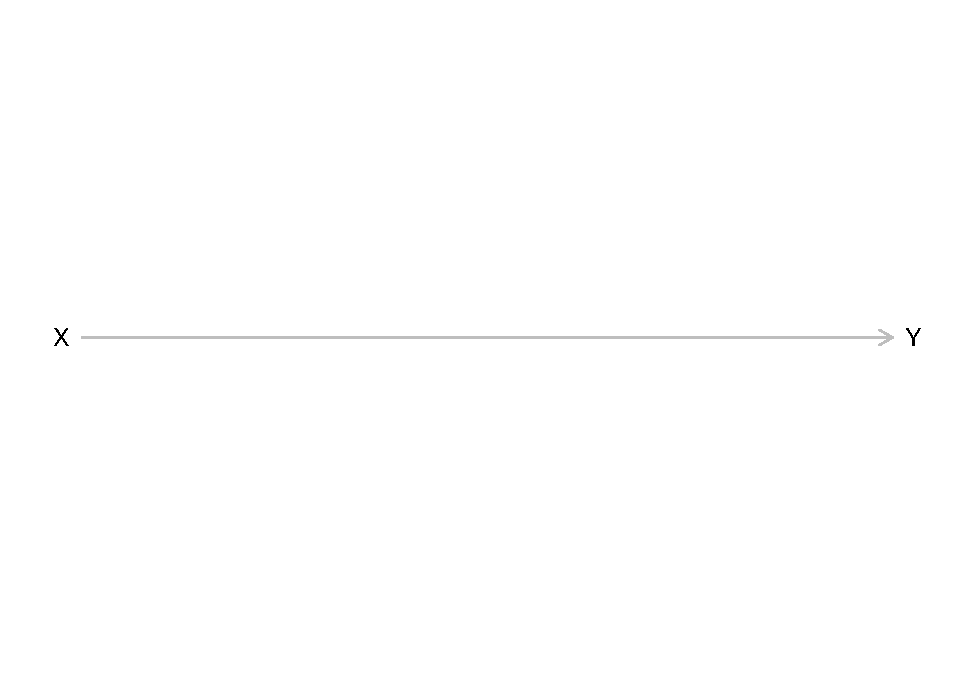
\includegraphics{_main_files/figure-latex/dag_directed-1.pdf}

What are the assumptions about the data generating process we have
encoded here? We have one dependent variable \(X\) that we assume to have
a direct effect on the independent variable \(Y\). We know that our
assumption was that \(X\) has an effect on \(Y\) and not the other way
around, because the arrow is \emph{directed} from \(X\) to \(Y\).

We call the sequence of one or many arrows that do not pass a single
variable more than once a \emph{path}. When trying to estimate an effect of
interest we are foremost interested in the paths going from our
independent variable of interest to the dependent variable. In the first
example we only have the one path \(X \rightarrow Y\), but in most ``real''
DAGs we will have multiple paths between \(X\) and \(Y\).

Consider this DAG, where we introduce a second variable \(A\):

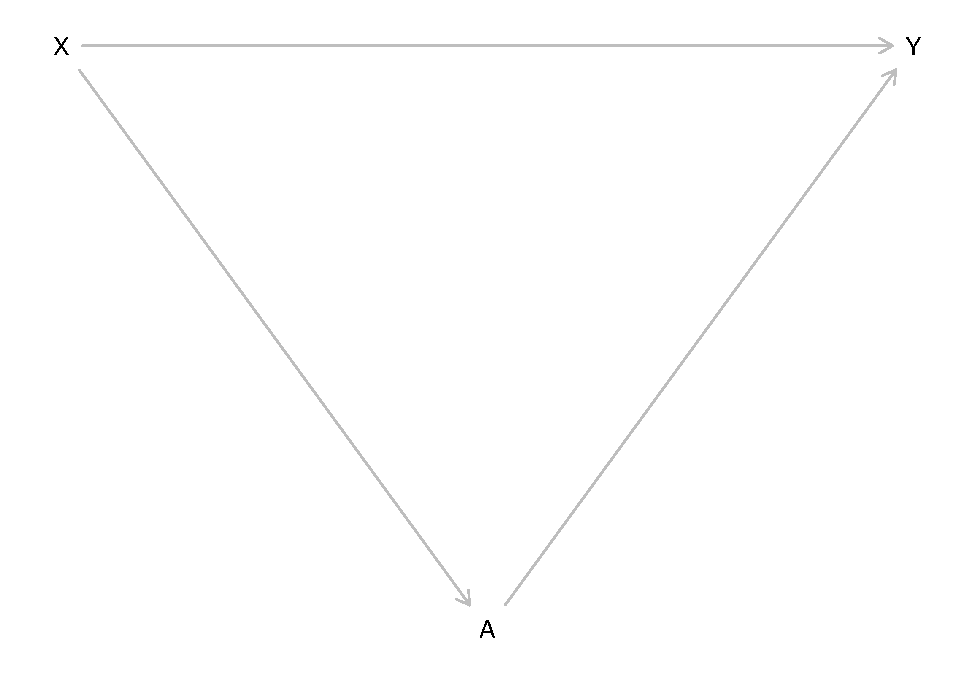
\includegraphics{_main_files/figure-latex/dag_paths-1.pdf}

Here there are two paths from \(X\) to \(Y\), \(X \rightarrow Y\) and
\(X \rightarrow A \rightarrow Y\). Our assumption here was that \(X\)
directly influences \(Y\), but that \(X\) also directly influences \(A\) which
in turn directly influences \(Y\). The latter is an indirect effect from
\(X\) on \(Y\) through \(A\).

DAGs are also \emph{acyclical}, meaning that there can not be any cyclical
relationships between variables. A cyclical relationship would be
present if we start from one variable and follow a path that leads us
back to this variable.

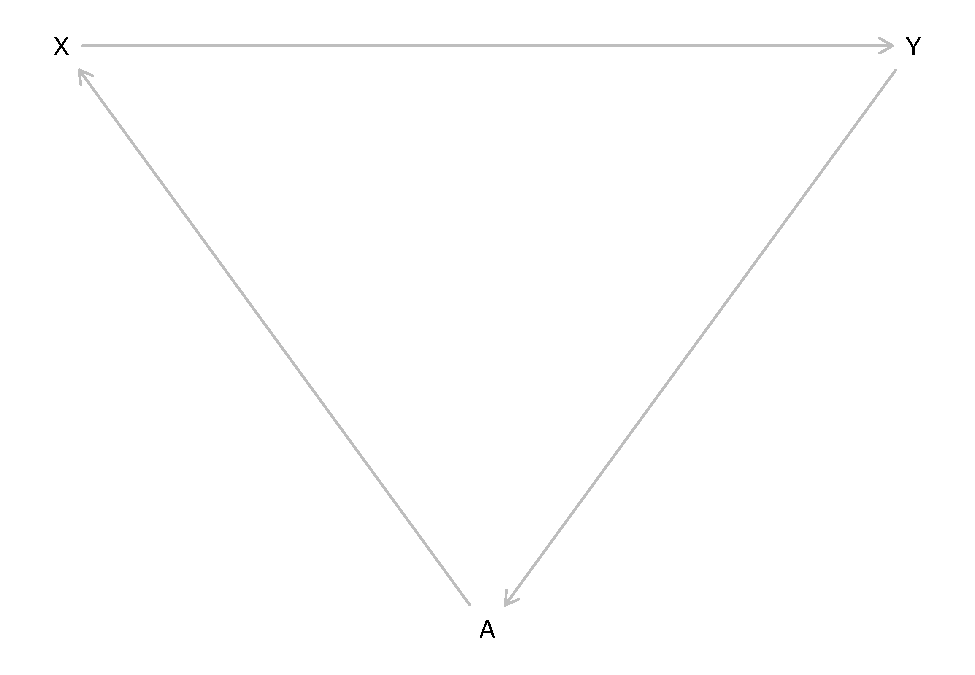
\includegraphics{_main_files/figure-latex/dag_acyclical-1.pdf}

In this example there is a path
\(X \rightarrow Y \rightarrow A \rightarrow X\) that leads us from \(X\)
back to \(X\). This is not allowed in a DAG.

Now that we know the basics, what do we actually do with a DAG? A DAG is
a way to graphically formalise our assumptions about the data generating
process. But it is about more than drawing nice formalisations, it is
also about figuring out which variables we have to include and which we
are not allowed to include to get an unbiased estimate of our effect of
interest. We do this by \emph{blocking} all paths from \(X\) to \(Y\) that do not
represent the relationship we want to estimate and at the same time
opening up all paths that do. For this to make sense, we need to know
the three patterns of relationships between a set of three variables and
how we can open or close paths with them.

\hypertarget{patterns-of-relationships}{%
\subsection{Patterns of relationships}\label{patterns-of-relationships}}

\hypertarget{chainspipe}{%
\subsubsection{Chains/Pipe}\label{chainspipe}}

Three variables can be connected in a \emph{chain} or \emph{pipe} like this:

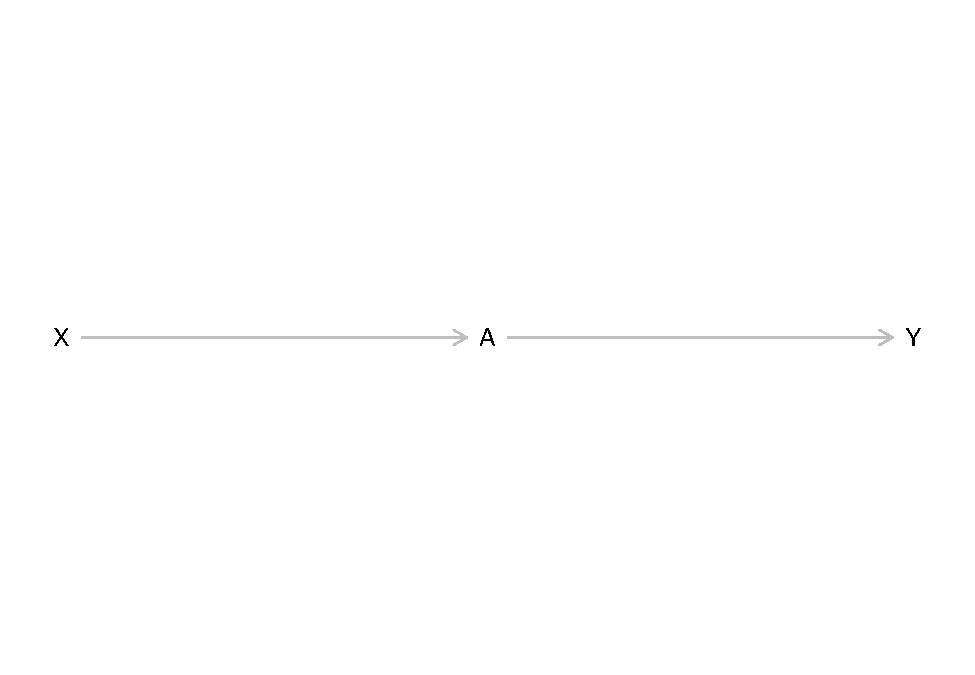
\includegraphics{_main_files/figure-latex/dag_pipe-1.pdf}

\(X\) has an effect on \(A\) which in turn affects the value of \(Y\). This
implies that \(X\) and \(Y\) are statistically correlated. When the value of
\(X\) changes, the value of \(Y\) also changes, ``transmitted'' by the
indirect effect \(X\) has on \(Y\) through \(A\). Remember we are still
interested in measuring the effect of \(X\) on \(Y\), so we also want to
measure this indirect effect.

The DAG tells us that there is a relationship between all three
variables. We therefore could be tempted to include \(A\) in our model as
well. But what would happen is that by including \(A\) we would \emph{block}
the path between \(X\) and \(Y\). We would not be able to measure the
association we are actually interested in. Including such a variable and
thereby blocking a path of interest is called \emph{overcontrol bias}.

In some cases overcontrolling can make the effect of interest
unmeasurable. We would then conclude from our analysis that \(X\) has no
effect on \(Y\) and that our hypotheses was wrong, while there actually
could be an effect that we made ``disappear'' by blocking its path.
Drawing a DAG based on our assumptions helps us to prevent this pitfall.

\hypertarget{mediation}{%
\paragraph{Mediation}\label{mediation}}

A special case of pipes is \emph{mediation}. We will only take about this
briefly here and return to the topic in \protect\hyperlink{med}{session 10}.

Consider this DAG:

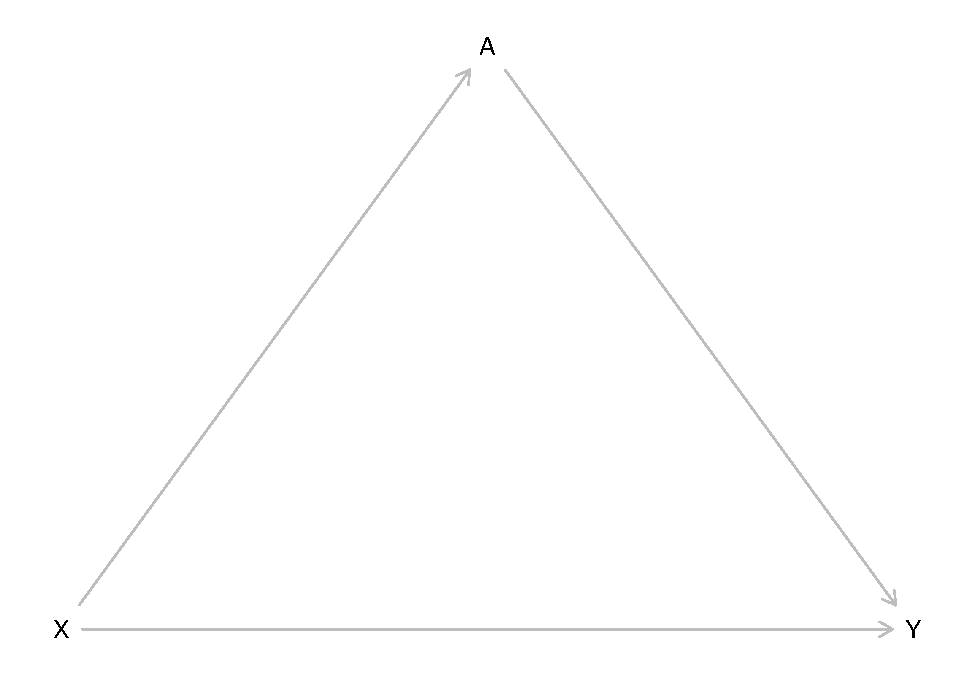
\includegraphics{_main_files/figure-latex/dag_mediation-1.pdf}

We see a direct effect through the path \(X \rightarrow Y\) as well as
indirect effect through \(X \rightarrow A \rightarrow Y\). Should we
include \(A\) in our model? This depends on what we want to measure.

If we are interested in the \emph{total effect} of \(X\) on \(Y\), we should not.
Both effects, the direct and the indirect paths, are of interest here,
so we keep both paths open by not controlling for \(A\).

Our interest could also lie exclusively in the \emph{direct effect}. Here we
would want to measure the effect of \(X\) stripped by all indirect
effects. In this case we want the path \(X \rightarrow Y\) to keep open,
but we would close the path \(X \rightarrow A \rightarrow Y\) by
controlling for \(A\).

We could also only be interested in the \emph{indirect effect}, the effect of
\(X\) on \(Y\) that goes through \(A\). We can not directly model this, but we
can compute the indirect effect as the difference between total and
direct effect.

\hypertarget{confounders}{%
\subsubsection{Confounders}\label{confounders}}

The second pattern we may see is the \emph{fork} or \emph{confounder}.

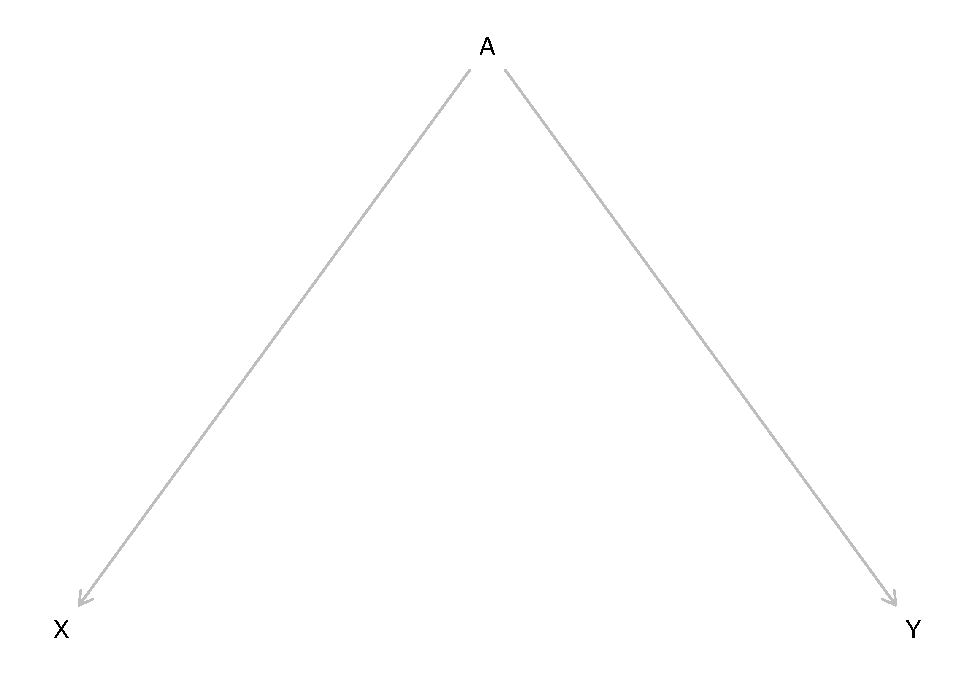
\includegraphics{_main_files/figure-latex/dag_confounder-1.pdf}

We see that there is no implied direct relationship between \(X\) and \(Y\)
but that both variables are influenced by \(A\). If we would measure the
relationship between \(X\) and \(Y\) we \emph{should} see no statistical
correlation. The problem is, that we \emph{would} see a correlation despite
this. Why is that? The values of \(X\) and \(Y\) both depend on the value of
\(A\). If we for example assume that both effects are positive the value
of \(X\) would rise with the value of \(A\) and the value of \(Y\) would rise
with the value of \(A\) also. The opposite would be true if both effects
were negative. Lower values for \(A\) would lead to lower values for \(X\)
and \(Y\). But even if the effects would be opposite, they would never
cancel each other out perfectly. \(X\) and \(Y\) vary together. If we just
include \(X\) and \(Y\) in our model this would show up as an effect from
\(X\) on \(Y\).

In DAG terms, there is an open path between \(X\) and \(Y\) although we did
not draw a direct path: \(X \leftarrow A \rightarrow Y\). This may seem
counterintuitive at first, as the arrows go in opposite directions, but
for paths in a DAG to exist, the direction of the arrows does not
matter. Every connection between variables is a path. So there is an
open path, in this case a so called \emph{backdoor path}, that leads to a
statistical association between \(X\) and \(Y\), but we can close it by
controlling for \(A\). If we do this, we would see no remaining
association between \(X\) and \(Y\) and thus get an unbiased estimate for
the effect of interest, i.e.~no effect.

If this still seems unintuitive consider the following example, which
you can also find in many statistical textbooks. Do storks bring babies?
We could tackle this analytically by taking a measure of babies born in
a region as our dependent variable and the number of storksightings in
the same region as our dependent variable. Let statistics come to the
rescue and help us discard the notion of the baby bringing stork once
and for all. But alas, our model will tell us that there is a positive
effect from storksightings on the number of newborns. Should we conclude
that everything we learned from our parents and teachers was one big lie
to hide away the magical truth about reproduction? Before we do that,
let us return to rationality. Maybe we have missed something important.
It turns out that there is a confounder we did not include in our model.
More rural areas have higher birthrates and also have a higher rate of
storksightings while both variables have lower values in more urban
regions. Our dependent and independent variables both vary by the value
of the confounder and thus it seems that there is a correlation where
there actually is none. If we now include a measure for the type of
region, let us say population density, this spurious association
disappears and we can return to normality. Storks do not bring babies
after all.

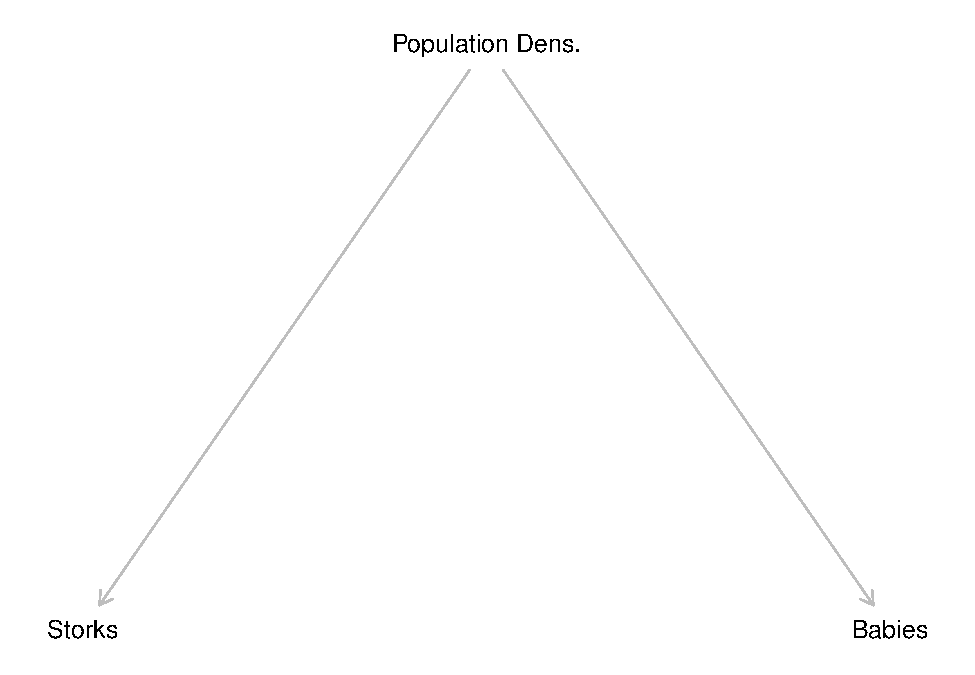
\includegraphics{_main_files/figure-latex/dag_storks-1.pdf}

\hypertarget{colliders}{%
\subsubsection{Colliders}\label{colliders}}

The last pattern we have to consider are \emph{colliders}. A collider is a
variable on a path that has two arrows pointing into it:

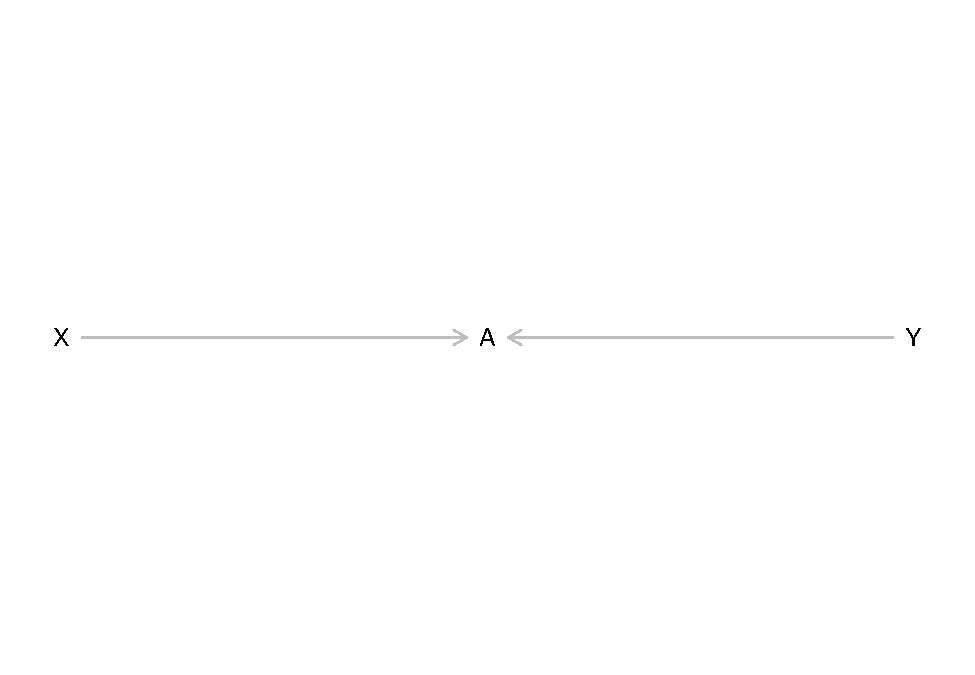
\includegraphics{_main_files/figure-latex/dag_mediation_1-1.pdf}

Here \(A\) is influenced by the value of \(X\) as well as \(Y\). Again, there
should be no effect of \(X\) on \(Y\) and in this case there is none if we
just include \(X\) and \(Y\) in our model. If we also include \(A\) we
introduce an association between \(X\) and \(Y\) even if there should be
none. This implies that we should not control for colliders because we
would open up a path that creates a spurious association between two
variables that are not related.

\hypertarget{adjustment-set}{%
\subsection{Adjustment set}\label{adjustment-set}}

Now we have all the building blocks for identifying which variables we
have to include in our model and which we are not allowed to include. If
we do not follow these rules we may statistically find relationships
where there are none or miss relationships that actually exist. We then
would draw the wrong conclusions for our hypotheses and research
question. We would produce bad science.

If we draw out our DAG and use its implications to identify the correct
\emph{adjustment set} \(Z\) of control variables, we do not fall into this
trap. We only control what we have to, and nothing that we should not.
We thus create the best model to get an unbiased estimate for our effect
of interest; but there is always a caveat and this is a big one. The
model is only correct if our DAG is also correct and we can never know
for certain if it is. We could make wrong assumptions, forget important
relationships, and make all matters of mistakes while building our DAG.
While DAGs are a great tool for identifying the adjustment set, the
technique alone can never replace careful thinking.

\hypertarget{nba-dag}{%
\section{NBA DAG}\label{nba-dag}}

We will now pick up where we left off in session 2 and return to the NBA
data. Equipped with our new tool we can now draw a DAG with the goal of
building a model to estimate the effect of points scored on the salary a
player receives. The assumption is, that the higher the point average,
the higher the salary. This makes intuitive sense as a high scoring
player is more valuable to the team and thus may receive a higher
monetary compensation.

Let us start building a DAG with the information we already have.

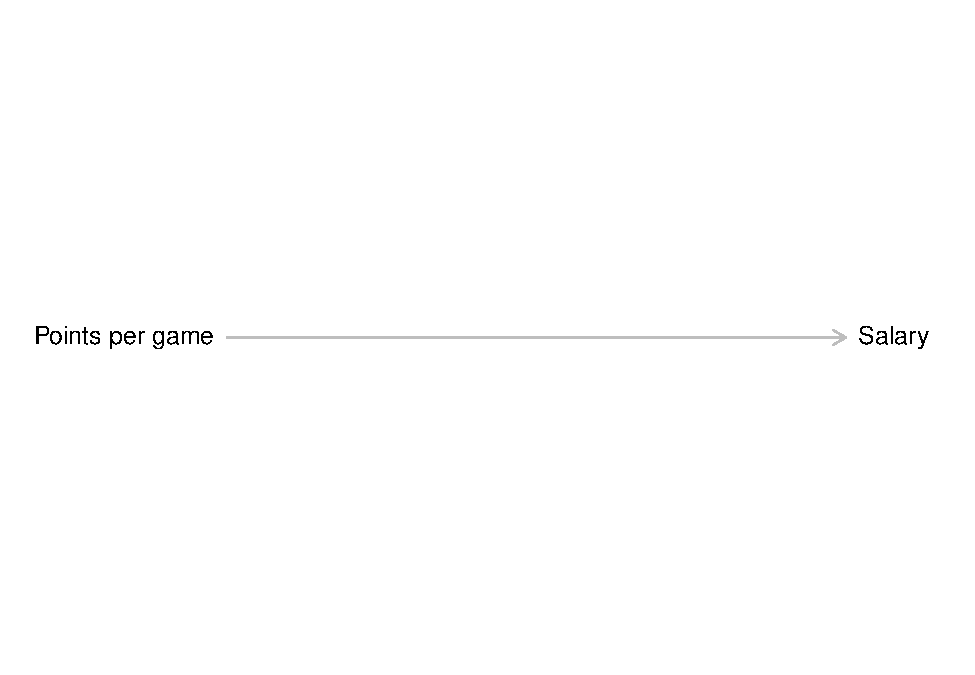
\includegraphics{_main_files/figure-latex/dag_1-1.pdf}

Now we have to think about other factors that could influence the
relationship between points and salary. One variable we already
identified as having an effect on both was the position a player
occupies. The position influences how many points per game a player can
score and we also already saw that centers make more money compared to
point guards. Right now we have no reason to believe that other
positions do not also have an effect on the received salary. Following
this reasoning, position is a confounder for points and salary.

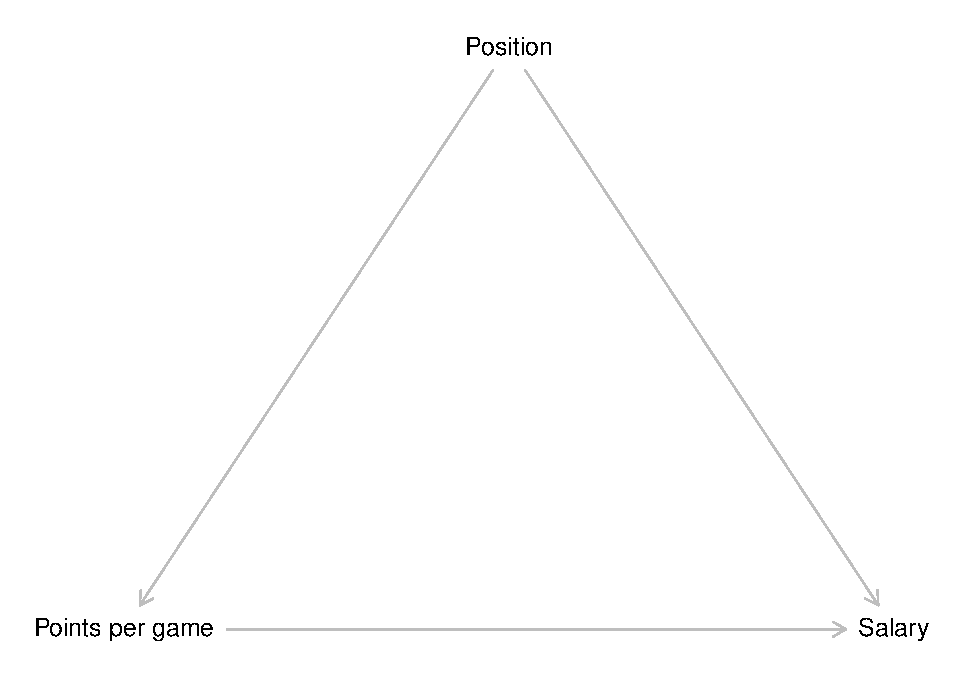
\includegraphics{_main_files/figure-latex/dag_2-1.pdf}

It is also reasonable that body height influences which position a
player can occupy. Centers have to be big while smaller players tend to
play on other positions. At the same time, height is an advantage if you
want to score in a basketball game. Thus height is a confounder for
points and position.

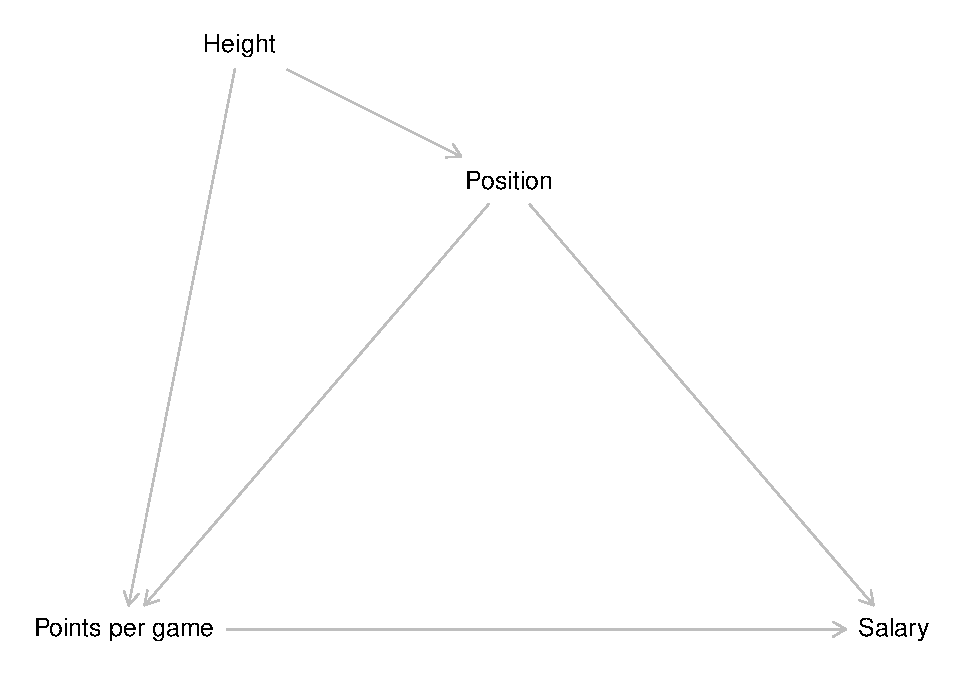
\includegraphics{_main_files/figure-latex/dag_3-1.pdf}

Another factor that will have an effect on the salary is the team a
player plays for. More successful teams will be able to pay higher
salaries. The season an observation was recorded in should also
influence the paid salary as we can expect a general inflation of
salaries over time.

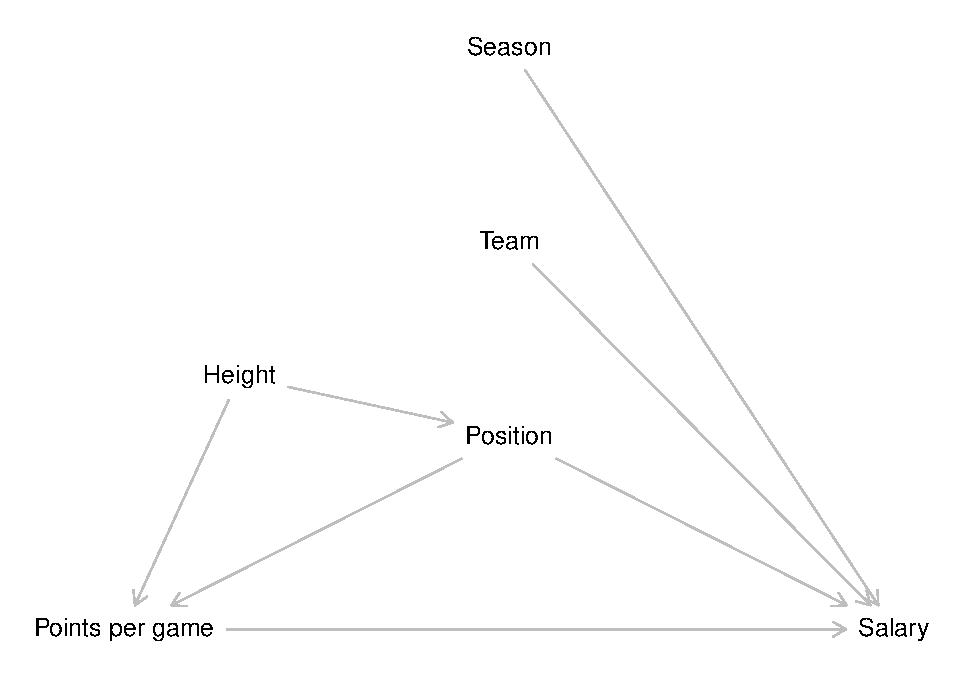
\includegraphics{_main_files/figure-latex/dag_final_0-1.pdf}

This is our final DAG. Does it correctly depict the underlying data
generating process? We do not know for sure, but the DAG correctly
reflects our assumptions at this point. Those may be wrong. Maybe the
data generating process actually works slightly or even completely
different; but to the best of our current knowledge, this is how the
scored points affect the salary a player receives.

We can now inspect what implications the DAG has for our model. To do
this, let us list the paths from our independent to the dependent
variable.

\[A: Points \rightarrow Salary\]
\[B: Points \leftarrow Position \rightarrow Salary\]

\[C: Points \leftarrow Height \rightarrow Position \rightarrow Salary\]
Path A is a direct path from our independent variable to our dependent
variable. We will have to include scored points and salary into our
model, but that is a given.

Paths B \& C are both backdoor paths - these are easily spotable by an
arrow pointing into the independent variable - that we have to address
somehow. Let us consider B first. Position is a confounder for points
and salary. Above we already learned how to deal with this, we control
for it. This removes the spurious part of the association between points
and salary introduced by the confounder. Path C also includes a
confounder, namely the body height of a player. Do we also control for
this variable to close path C? No, we do not. If we further examine path
C we will see that it also includes position as a pipe. When we control
for a variable in a pipe, the path gets closed. As we have to include
position to close path B, path C is also already closed.

The two remaining variables, team and season, have direct effects on the
salary but do not lie on a path from points to salary. This implies,
that we do \textbf{not} have to control for them if our goal is estimating
the effect of points on salary.

Above we briefly talked about the two possible goals of modelling. Here
and over the next sessions our goal is estimating an effect of interest
without bias. We used the DAG to identify an adjustment set of variables
we have to control for to reach this goal. If our goal was predicting
the salary as accurately as possible we would made other conclusions.
The team a player is employed by and the season where an observation was
measured are both relevant predictors for the received salary. For
prediction we would have included both variables because this should
increase the accuracy of the prediction. We will return to this in more
detail in \protect\hyperlink{pm-t}{session 11}.

\hypertarget{resources}{%
\section{Resources}\label{resources}}

\hypertarget{dagitty.net}{%
\subsection{dagitty.net}\label{dagitty.net}}

While the underlying rules of DAGs are relatively straightforward,
identifying the adjustment set can get harder the more complex a DAG
gets. Consider this for instance:

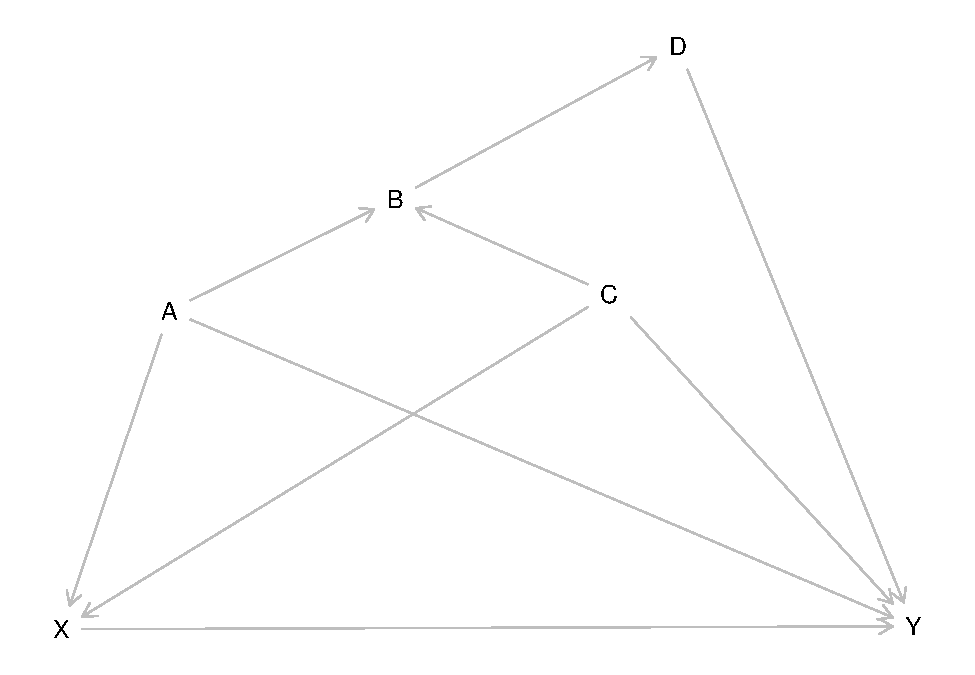
\includegraphics{_main_files/figure-latex/dag_final_1-1.pdf}

What variables do we have to include in our adjustment set to get
unbiased measure for the effect from \(X\) on \(Y\)? We would suggest you
take out pen and paper and try to figure it out. You can approach this
as above. List all paths from \(X\) to \(Y\) that do not include a variable
twice and try to find the adjustment set that closes all paths besides
the one(s) needed to measure the effect from \(X\) on \(Y\). Spoiler: In
this case the only path we want to keep open is the direct effect
\(X \rightarrow Y\).

While this is doable, you may be unsure if you found the correct set.
Luckily there is a convenient way to find out. \url{https://dagitty.net/}
provides a browser tool where you can draw DAGs - as well as export them
for your papers - and check for the correct adjustment set. After
launching the tool you should click on ``Model'' and then ``New model''. Now
you can start drawing. New variables are added by clicking on the canvas
and naming them, arrows are added by first clicking on the variable
where the arrow should start and then on the variable where it should
end. For everything to work you should also declare the independent
variable of interest the ``Exposure'' and the dependent variable the
``Outcome''. Both can be set on the left under ``Variable''. When the DAG is
drawn correctly, the top right panel ``Causal effect identification''
should show which variables need to be part of the adjustment set to
estimate the effect of interest.

Note that ``Causal effect identification'' is set to display the
adjustment set for the total effect. This also is what we are interested
in here. If we are interested in mediation, we can also set the panel to
display the set for the direct effect.

\hypertarget{how-to-use-dagitty}{%
\subsection{How to use dagitty()}\label{how-to-use-dagitty}}

We can also draw DAGs directly in R, using the \texttt{dagitty} package. To
start drawing a DAG we write \texttt{dagitty(\textquotesingle{}dag\ \{\})}. The actual definition
of the DAG takes place between the squirly brackets. First we list all
variables in the model by writing their names between quotation marks.
For each variable we can optionally add additional options between
square brackets following the name. In the example below we define one
variable as \texttt{exposure} and one as \texttt{outcome}, just like we would do on
dagitty.net. We also give values for the relative positions. If we skip
those, \texttt{dagitty()} will decide on the positions itself which may or may
not look nice and tidy. After all variables are defined we write out the
paths that should be present connecting the variable names with \texttt{\textless{}-} or
\texttt{-\textgreater{}}, depending on the direction an arrow should point. We can than use
\texttt{plot()} to see the DAG.

\begin{Shaded}
\begin{Highlighting}[]
\CommentTok{\# Load the dagitty package}
\FunctionTok{library}\NormalTok{(dagitty)}

\CommentTok{\# Define a DAG}
\NormalTok{dag }\OtherTok{\textless{}{-}} \FunctionTok{dagitty}\NormalTok{(}\StringTok{\textquotesingle{}dag \{}
\StringTok{  "Exposure" [exposure, pos="{-}1,0"]}
\StringTok{  "Outcome" [outcome, pos="1,0"]}
\StringTok{  "Confounding Variable" [pos="0,{-}1"] }
\StringTok{  "Mediator" [pos="0,1"]}
\StringTok{  "Exposure" {-}\textgreater{} "Outcome"}
\StringTok{  "Exposure" {-}\textgreater{} "Mediator" {-}\textgreater{} "Outcome"}
\StringTok{  "Exposure" \textless{}{-} "Confounding Variable" {-}\textgreater{} "Outcome"}
\StringTok{\}\textquotesingle{}}\NormalTok{ )}

\CommentTok{\# Plot the DAG}
\FunctionTok{plot}\NormalTok{(dag)}
\end{Highlighting}
\end{Shaded}

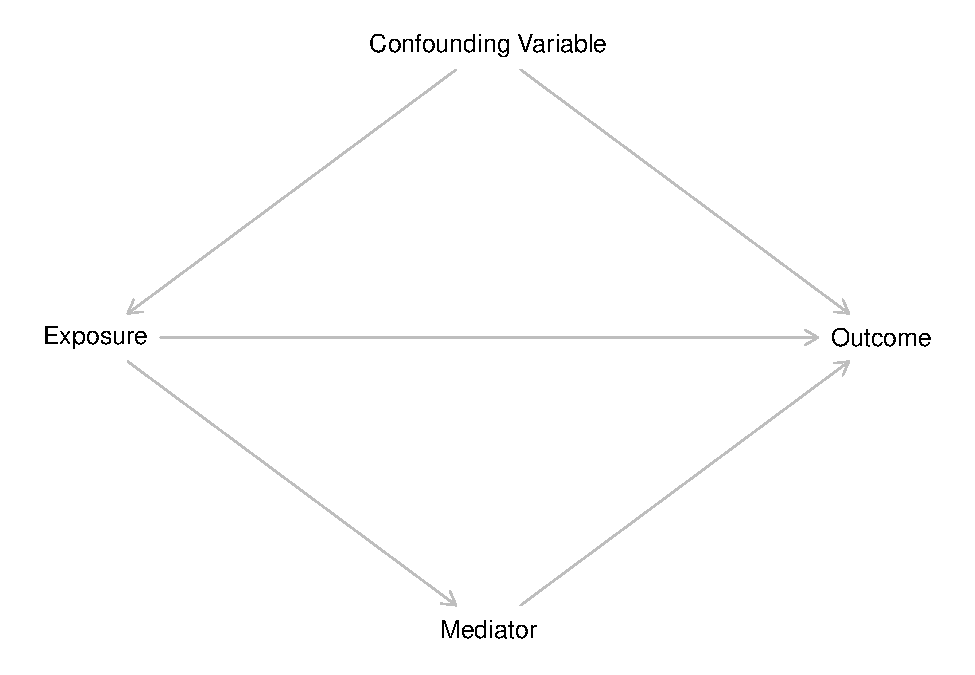
\includegraphics{_main_files/figure-latex/dagitty_example-1.pdf}

We can also use the function \texttt{adjustmentSets()} to derive our adjustment
set. The argument \texttt{effect\ =} lets us control if we want to see the
adjustment set for the \texttt{"total"} or \texttt{"direct"} effect.

\begin{Shaded}
\begin{Highlighting}[]
\CommentTok{\# Identify the minimal adjustment set for estimating the total effect of Exposure on Outcome}
\FunctionTok{adjustmentSets}\NormalTok{(dag, }\AttributeTok{effect =} \StringTok{"total"}\NormalTok{)}
\end{Highlighting}
\end{Shaded}

\begin{verbatim}
## { Confounding Variable }
\end{verbatim}

\begin{Shaded}
\begin{Highlighting}[]
\CommentTok{\# Identify the minimal adjustment set for estimating the direct effect of Exposure on Outcome}
\FunctionTok{adjustmentSets}\NormalTok{(dag, }\AttributeTok{effect =} \StringTok{"direct"}\NormalTok{)}
\end{Highlighting}
\end{Shaded}

\begin{verbatim}
## { Confounding Variable, Mediator }
\end{verbatim}

\hypertarget{more-on-dags}{%
\subsection{More on DAGs}\label{more-on-dags}}

If you are interested in diving deeper into DAGs, we can recommend this
resources, which were also used for writing this session.

Richard McElreath provides a great introduction into the topic with many
clear examples. While the book chapter on DAGs may require some
knowledge of advanced statistical topics, the corresponding lecture on
YouTube is more approachable:

McElreath, Richard (2020). Statistical Rethinking: A Bayesian Course
with Examples in R and STAN. Second Edition. Boca Raton \& Oxon: CRC
Press. Chapter 5: The Many Variables \& The Spurious Waffles, 123-160.

Corresponding YouTube lecture:
\url{https://www.youtube.com/watch?v=mBEA7PKDmiY}

\hfill\break

Felix Elwert wrote a concise paper on DAGs with a perspective that is
more focused on causality than we have presented here:

Elwert, Felix (2013). Graphical Causal Models. In S. L. Morgan (Hrsg.),
Handbook of Causal Analysis for Social Research, 245--273. Dordrecht
{[}u.a.{]}: Springer.

\hfill\break

If you really want to get into it, the work of Judea Pearl was central
for establishing DAGs. An approachable starting point would be the ``Book
of Why'':

Pearl, Judea \& Dana Mackenzie (2018). The book of why : the new science
of cause and effect. New York: Basic Books.

\hypertarget{lin-t-1}{%
\chapter{Linear Regression - Theory I: Simple Linear Regression}\label{lin-t-1}}

The next three sessions will comprise an introduction for linear regressions.
We will look at the theoretical underpinnings, the interpretation of results
and the underlying assumptions of these models. For this introduction we will
keep the NBA data aside and use some simulated data that plays nice with us.
We will return to the NBA data in session 8 applying everything we
learned to assess the effect of scored points on salary.

\hypertarget{objectives-2}{%
\section{Objectives}\label{objectives-2}}

\begin{itemize}
\tightlist
\item
  Understand simple linear regression
\item
  Understand the regression formula
\item
  Interpret the results
\end{itemize}

\hypertarget{what-is-linear-regression}{%
\section{What is Linear Regression}\label{what-is-linear-regression}}

As we eluded to last session, there are two main approaches to using
statistical modelling in the social sciences.
The more classical approach is to use modelling for estimating the effect that
one or several independent variables have on one dependent variable. Maybe we
are interested in knowing if a higher income has an effect on life satisfaction
and if yes, what the direction and magnitude of this effect is. Does more money
actually make you happier?

The other and more recent approach is to use modelling for making predictions
with high accuracy. Based on the relationships between many independent
variables and one dependent variable. We try to predict the latter for actual
or hypothetical cases based on their values for the independent variables.
This approach lies at the heart of \emph{machine learning} and drives many of the
technologies we use on a daily basis from E-Mail spam filters to ChatGPT.
Returning to the example above, we are not interested in measuring the \emph{effect}
of money on life satisfaction, but in \emph{predicting} the value for life satisfaction
based on money and a host of other variables as accurately as possible.

Linear regression is one of the many available modelling techniques and it can
serve both approaches. Over the next sessions we will focus on using
linear regression for estimating an effect of interest but we will return to
prediction in \protect\hyperlink{pm-t}{session 11}.

How do we know if we should choose linear regression for a specific task?
This is not easy to answer as there are many alternatives and even variations of
linear regression which may be better suited for a specific empirical problem.
As this is an introduction to modelling and time is of the essence we opted to
mainly focus on an in-depth introduction to linear regression.
This technique is suited for many problems and
is comparably easy to understand and use. Also, after learning the ins and outs
of linear regression, we are in a good position to build upon that knowledge and
learn all of those more complex and specific models that we will encounter in
textbooks and scientific papers.

With the pool of options trimmed down to one, the central question remains unanswered.
Should I use linear regression for my task? As we have no alternatives to chose
from, we can change the question to: Can I use linear regression for my task?
The answer mainly depends on what type of dependent variable we want to use.
If it is metric, we can use linear regression.
In our cases the dependent variable is metric, as you will find out below.
If we had other types of dependent variables we would have to use different
models.
For example a common choice for binary or categorical dependent variables is
logistic regression, which we will introduce at a \protect\hyperlink{log-est}{later point in the course}.

\hypertarget{examplary-research-question-data}{%
\section{Examplary research question \& data}\label{examplary-research-question-data}}

For this introduction, let us imagine that we are interested in a research
question that asks: \emph{What makes a good grade in a seminar paper?} In particular we
are interested in the effect that the hours a student invests in working on it
has on the grade. Based on some theoretical considerations, and maybe some
idealistic views, we derive our main hypotheses that putting in more hours will
result in a better grade.

Now we also - hypothetically - held a small survey and asked 200 imaginary
students some questions on how they approached writing a seminar paper. In
particular we asked them how much time they spent working on the paper, if they
have attended (almost) all seminar sessions, how closely they worked with their
lecturers in preparing the paper and what the mean grade for previous papers
was. As these imaginary students have already turned in their papers, we also
know the grades they achieved.

Please note, that this is data on \textbf{imaginary} students, meaning we have
simulated the data making some assumptions on how to achieve a good (or bad)
grade in a paper. The assumptions we made do not necessarily reflect the way
\emph{you} write a good paper, while still being based in our experience on what it
takes to achieve a good grade. But remember, no real students were harmed in
making up this data.

Let us have a first look on the data:

\begin{verbatim}
## -- Data Summary ------------------------
##                            Values
## Name                       grades
## Number of rows             200   
## Number of columns          7     
## _______________________          
## Column type frequency:           
##   factor                   1     
##   logical                  1     
##   numeric                  5     
## ________________________         
## Group variables            None  
## 
## -- Variable type: factor -------------------------------------------------------
##   skim_variable n_missing complete_rate ordered n_unique
## 1 contact               0             1 FALSE          3
##   top_counts               
## 1 No : 80, In : 70, E-M: 50
## 
## -- Variable type: logical ------------------------------------------------------
##   skim_variable n_missing complete_rate  mean count            
## 1 attendance            0             1 0.765 TRU: 153, FAL: 47
## 
## -- Variable type: numeric ------------------------------------------------------
##   skim_variable            n_missing complete_rate      mean    sd     p0    p25
## 1 grade                            0             1  2.97e+ 0 1.08    1     2.1  
## 2 hours                            0             1  4.03e+ 1 6.29   23    36    
## 3 previous_grades                  0             1  2.94e+ 0 0.965   1     2.3  
## 4 previous_grades_centered         0             1 -7.21e-17 0.965  -1.94 -0.635
## 5 hours_centered                   0             1  1.70e-15 6.29  -17.3  -4.33 
##       p50   p75  p100 hist 
## 1  3       3.73  5    ▅▆▇▆▅
## 2 41      45    57    ▁▅▇▅▁
## 3  2.95    3.62  5    ▅▇▇▆▂
## 4  0.0150  0.69  2.06 ▅▇▇▆▂
## 5  0.670   4.67 16.7  ▁▅▇▅▁
\end{verbatim}

Right now, the observations are ordered by the grade of the seminar paper which
run from \(1.0\) to \(5.0\) in increments of \(0.1\). While this is somewhat
unrealistic - the German grading system actually only uses the increments \(.0\),
\(.3\) and \(.7\) - simulating the data in this way will make the demonstrations on
linear regression easier and more straightforward. The variable
\texttt{previous\_grades} is set up in the same way and represents the mean of the
grades the student received up to this point. \texttt{hours} represents the time a
student spent on writing the paper, ranging from \(23 - 57\) hours, with a mean of
about \(40\). Besides these metric variables, the data set also contains two
categorical measures. \texttt{attendance} is a \emph{binary} or \emph{dummy variable}, meaning it can only
have the values \(1\) or \(0\) or \texttt{TRUE} and \texttt{FALSE} in this case, as it is saved as
a logical variable. \texttt{TRUE} represents that a student attended almost all seminar
sessions before writing the paper - which about \(77%
\) did -, \texttt{FALSE} states that
they did not.
\texttt{contact} is a factor variable with three categories and shows the answers to
the imaginary question on how much contact the student had to the lecturer
before starting the writing process. Besides \texttt{No\ contact} the students could
have had \texttt{E-Mail} contact to state their research question and get some short
written feedback or meet the lecturer \texttt{In\ Person} to achieve a deeper discussion
of the question and the laid out plan for writing the paper.
The two additional variables are versions of \texttt{previous\_grades} and \texttt{hours} that
are centered on their respective means. They will come into play at a later
point in this session.

Let's have a look at some observations.

\begin{verbatim}
## # A tibble: 10 x 7
##    grade hours previous_grades attendance contact   previous_grades_centered
##    <dbl> <int>           <dbl> <lgl>      <fct>                        <dbl>
##  1     1    50             1.4 TRUE       E-Mail                      -1.54 
##  2     1    46             1   TRUE       E-Mail                      -1.94 
##  3     1    42             1   TRUE       In Person                   -1.94 
##  4     1    49             1   FALSE      In Person                   -1.94 
##  5     1    42             1.2 TRUE       In Person                   -1.74 
##  6     1    46             1.8 TRUE       In Person                   -1.14 
##  7     1    44             1.4 FALSE      In Person                   -1.54 
##  8     1    45             2   TRUE       In Person                   -0.935
##  9     1    48             1   TRUE       In Person                   -1.94 
## 10     1    45             2   TRUE       In Person                   -0.935
## # i 1 more variable: hours_centered <dbl>
\end{verbatim}

From this first 10 rows, we can see that the students with the best grades spent
more than 40 hours on writing, have already achieved good grades in their papers
up to this point and at least had some contact to the lecturers. Most also
regularly attended the seminar but two did not and still achieved a \(1.0\) in
their grade.

So what makes a bad grade?

\begin{verbatim}
## # A tibble: 10 x 7
##    grade hours previous_grades attendance contact    previous_grades_centered
##    <dbl> <int>           <dbl> <lgl>      <fct>                         <dbl>
##  1   4.8    37             4.2 TRUE       No contact                    1.27 
##  2   4.8    38             4.3 TRUE       E-Mail                        1.36 
##  3   4.8    35             4.4 TRUE       E-Mail                        1.47 
##  4   4.9    40             4.2 TRUE       E-Mail                        1.27 
##  5   5      35             3.9 FALSE      No contact                    0.965
##  6   5      41             4.9 TRUE       No contact                    1.97 
##  7   5      24             4.7 TRUE       E-Mail                        1.76 
##  8   5      33             5   TRUE       E-Mail                        2.06 
##  9   5      29             4.1 FALSE      E-Mail                        1.16 
## 10   5      50             4.6 FALSE      E-Mail                        1.66 
## # i 1 more variable: hours_centered <dbl>
\end{verbatim}

Here the picture seems less clear. While most students did not put in as many
hours, some did and still failed to pass. Half of the students that received a
\(5.0\) regularly attended and most at least had E-Mail contact before writing
their paper. What seems to be more consistent though is that the mean of the
previous grades is rather low.

So what do we know now? Does a good or bad track record in grades predict all
future grades? This seems not only unrealistic but is also a kind of sad take home
message. To get a better understanding on which of the potential influential
variables has an effect on the final grade and what the magnitude and direction
of these effects is, we now turn to linear regression.

\hypertarget{simple-linear-regression}{%
\section{Simple Linear Regression}\label{simple-linear-regression}}

In a \emph{simple linear regression}, the model is used to describe the relationship
between \emph{one} dependent and \emph{one} independent or explanatory variable. The
question this model can answer for us is: By how much does the dependent
variable increase or decrease, when the explanatory variable increases by \(1\)?

Returning to our exemplary research question on what makes a good grade in a
seminar paper, an intuitive hypotheses would be that the grade gets better the
more hours a student invests in writing the paper. In this case we assume a
linear relationship between the independent variable \texttt{hours} and the dependent
variable \texttt{grade}. As German grades are better the lower their value, we thus
would assume a negative effect from \texttt{hours} on \texttt{grade}.

Before turning to the formalities and practical application of a simple linear
regression model, let us first have a look on this relationship by plotting the
variables against each other.

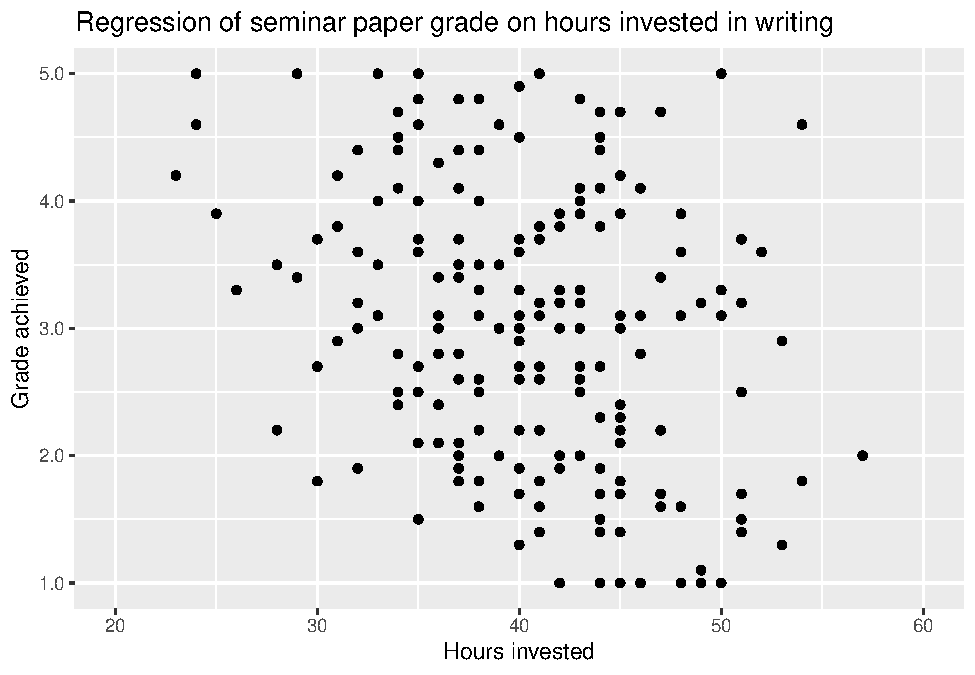
\includegraphics{_main_files/figure-latex/plot_grade_hours-1.pdf}

When we are talking about dependent and independent variables, there is the
convention to plot the former on the y-axis and the latter on the x-axis. So the
\emph{y-variable} is to be explained and the \emph{x-variable} is used to explain it.
This convention will also be used in all formulas in this seminar.

Looking at the plot we first see a cloud of dots, representing all combinations
of \texttt{hours} and \texttt{grade} in all our \(200\) observations. It may be hard to pick out
any pattern, but looking closely we can observe that overall the dots seem to
follow a downward slope from the upper left - indicating few hours worked and a
worse grade - towards the lower right - indicating more invested hours and a
better grade. This would be the relationship stated in our hypotheses. The more
hours a student works on a seminar paper the better the final grade will be.

We can try to describe this pattern by adding a line from the upper left to the
lower right.

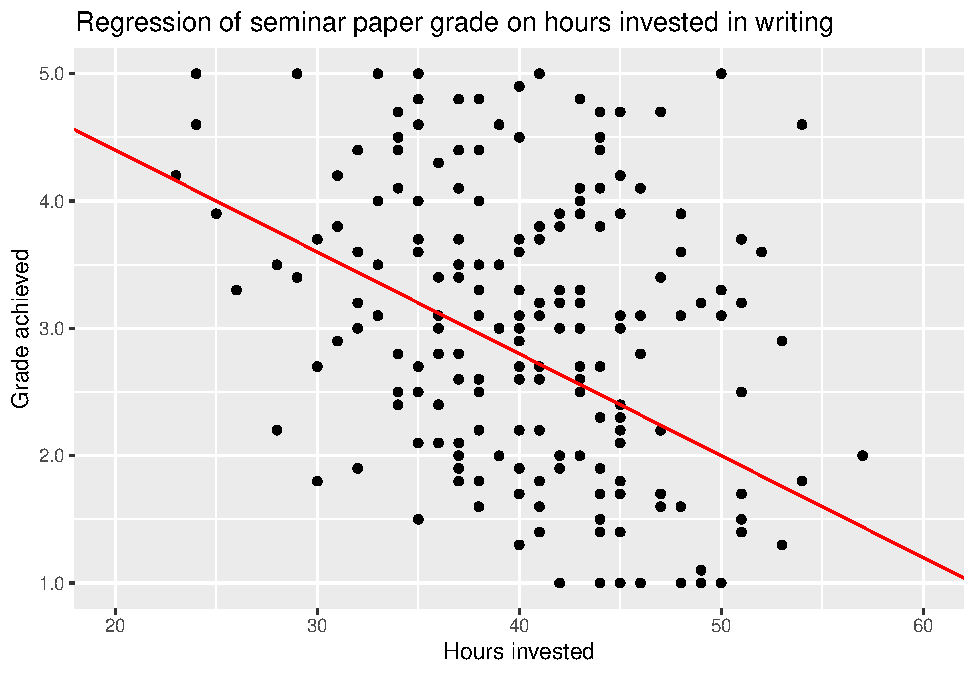
\includegraphics{_main_files/figure-latex/plot_grade_hours_wild_guess-1.pdf}

This describes the relationship between the two variables as linear. Each hour
invested decreases the grade by a certain amount, for this proposed line by
exactly \(0.08\) points. Remember that decreasing the value of the grade actually
means getting a better grade.

But is this the only possible line or even the \emph{correct} one? Most certainly not,
as the values used to draw the line were only a wild guess. We
could imagine several other lines that also look more or less reasonable - as
well as some that look unreasonable - and add them to the plot.

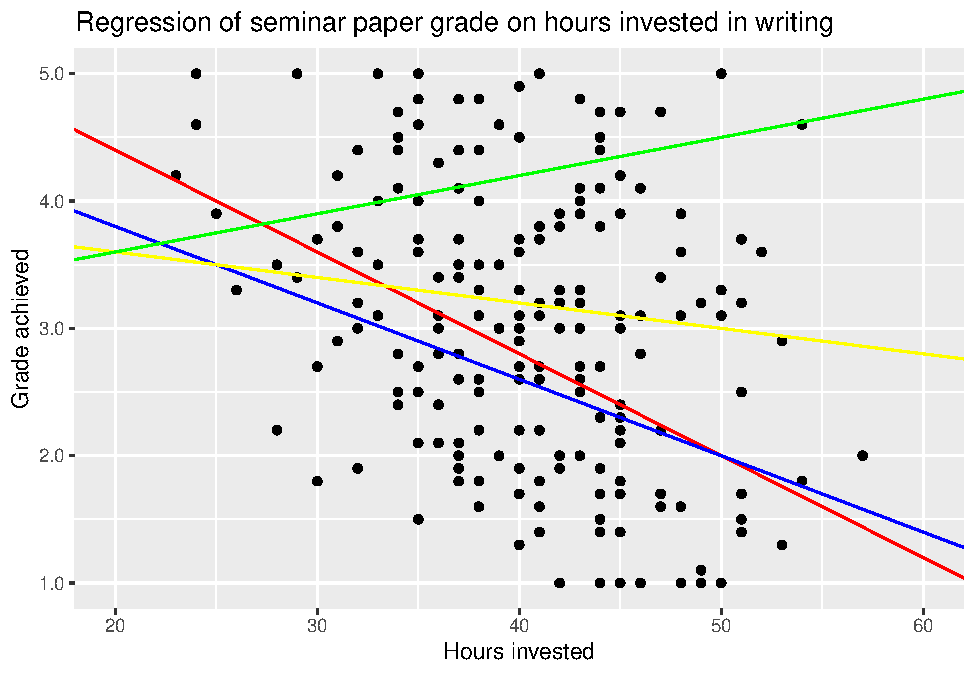
\includegraphics{_main_files/figure-latex/plot_grade_hours_wild_guesses-1.pdf}

While we have some intuition that the green line completely misses the mark, we
can't really decide between the others just by looking at the plot. The
data points are way to dispersed to see the relationship clearly.

The goal of using a simple linear regression model is to identify the \emph{one} line
that describes the relationship the best. Here \emph{best} means, with as little
error as possible.

\hypertarget{regression-formula}{%
\subsection{Regression Formula}\label{regression-formula}}

To understand how these lines in the above plot were conceived and how to find
the line with the best \emph{fit}, i.e.~the lowest error, we have to understand the
formula for linear regression. While formulas may always be kind of daunting,
we are in luck as this particular one is actually quite easy to understand,
especially when paired with a graphical representation.

\[y = \beta_0 + \beta_1*x_1 + \epsilon\]

Let us first look at the parts we already know. \(y\) is the dependent variable,
in our case the grade achieved. So one thing is for sure, the whole right part
of the equation has to be used to calculate the value of \(y\) from the data, i.e.
from the dependent variable \(x\). Here we have three terms. Let us skip the first one
for now and focus on the second one \(\beta_1*x_1\).

\(x_1\) is the dependent variable, in our case \texttt{hours}. \(\beta_1\) is the
\emph{regression coefficient} for \(x_1\). This value gives us the \emph{slope} of the
regression line. Based on this, we can start rewriting the general formula and
tailor it to our specific use case.

\[y_{grade} = \beta_0 + \beta_{hours}*x_{hours} + \epsilon\]

Let us return to the first wild guess we made above.

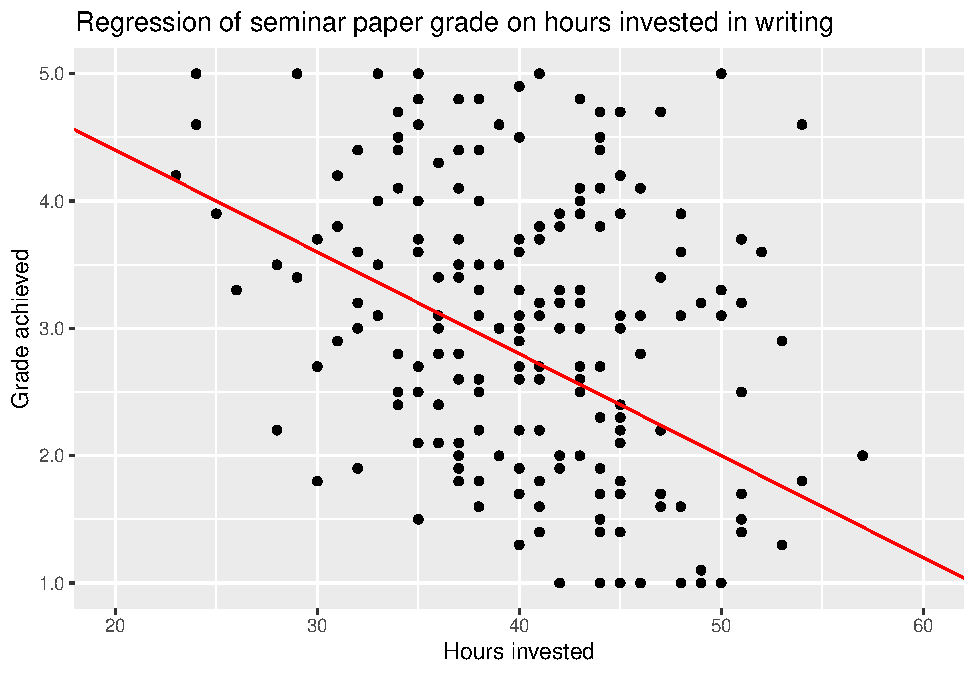
\includegraphics{_main_files/figure-latex/plot_grade_hours_wild_guess_expl_slope-1.pdf}

Here we guessed that an increase in invested time of one hour decreases the
value of \texttt{grade} by \(0.08\). This is the slope of the red line and thus also the
coefficient in the regression formula that is used in computing said line. So,
\(\beta_{hours} = -0.08\). We can insert this value into our formula.

\[y_{grade} = \beta_0 -0.08*x_{hours} + \epsilon\]

In this way the value of \(x_{hours}\) is multiplied by \(-0.08\). Let us assume a
student worked \(40\) hours on their paper. \(-0.08*40\) being \(-3.2\), we assume that
working 40 hours on a paper \emph{on average} - more on that later - leads to a \(3.2\)
lower grade value. But \(3.2\) lower than what?

Looking at the formula again, we see that we subtract this value from \(\beta_0\).
This is the \emph{intercept}, the value at which the line intersects with the y-axis.
Let us zoom out on our plot to see what happens.

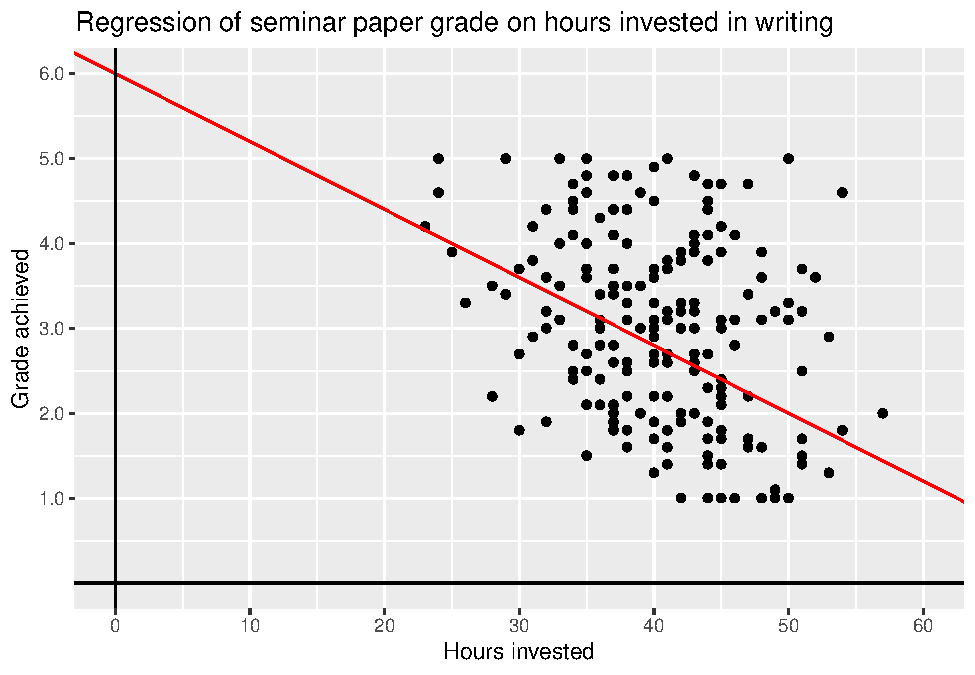
\includegraphics{_main_files/figure-latex/plot_grade_hours_wild_guess_expl_intercept-1.pdf}

We can now see the point where the red line intersects with the y-axis. This is
the intercept of this line, i.e.~\(\beta_0 = 6\).

\[y_{grade} = 6 -0.08*x_{hours} + \epsilon\]

If we now again assume a time investment of \(40\) hours, we can compute
\(6-0.08*40 = 2.8\). So our red regression line - which is still only a wild guess
- assumes, that working 40 hours on a seminar paper will result in a grade of
\(2.8\), on average. We can mark these values in our plot:

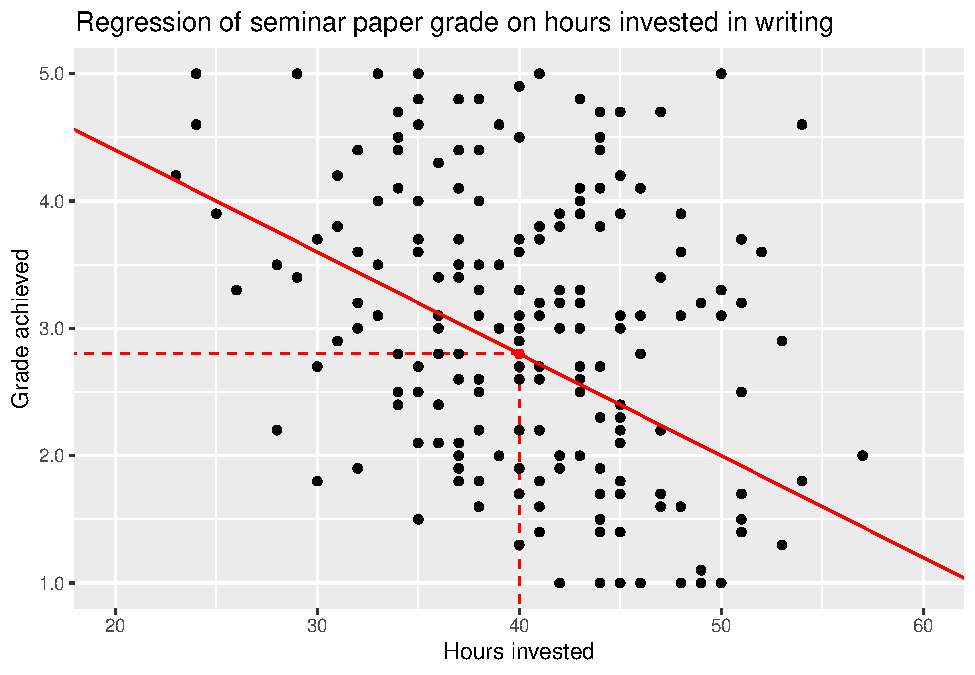
\includegraphics{_main_files/figure-latex/plot_grade_hours_wild_guess_expl_40hours-1.pdf}

The red dot is the intersection of the values \texttt{hours\ =\ 40} and \texttt{grade\ =\ 2.8}.
As this is the value for \(y\) our regression line assumes a student with a time
investment of 40 hours achieves, the red dot also lies exactly on the red line.

But if we look at the plot once again, we can see that most actual observations
for students that invested 40 hours do not actually lie on the regression line
but are scattered above and below the line. Some of these students achieve
much worse or much better grades than \(2.8\) investing the same amount of time in
their work. This leads us to the last part of the formula, \(\epsilon\).

This is the \emph{error term}. Having data that is dispersed like this - and any real
world data will always be - our linear line will never be able to pass exactly
through every data point. Some points may lie exactly on the line, but many or
most will not.

We can visualize this. To keep the plot readable, we only do this for some
random observations but in reality the distance of every data point from the
regression line is taken into account.

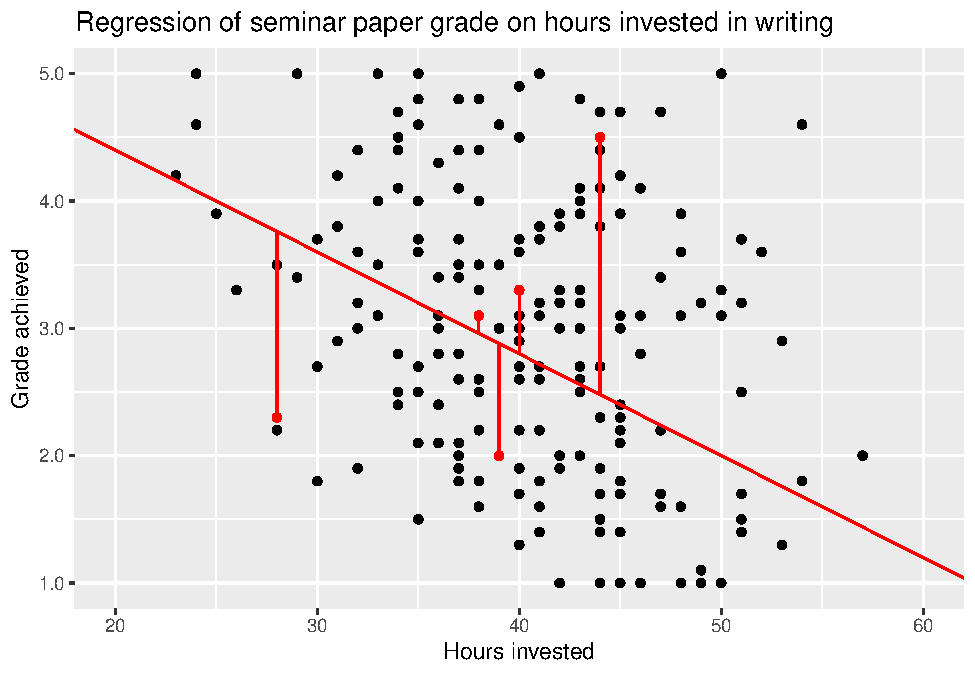
\includegraphics{_main_files/figure-latex/plot_grade_hours_wild_guess_expl_residuals-1.pdf}

The distance of these or rather all points from the line, the \emph{residuals}, are
represented in the error term \(\epsilon\). It is a measure for how wrong our line
is in describing the data in its entirety. So why is it wrong? We can not say
for sure, but there are two common main reasons.

For one, there may be other variables that also influence the relationship
between invested hours and achieved grade, something that we will return to
in the \protect\hyperlink{lin-t-2}{next session}, when we expand the idea of linear regression to multiple
independent variables.

But there is also random variation present in every bit of real world data.
While our data is simulated, we also added random variation on purpose. Because
this is what real world data is, it is messy and it is noisy.

Not every seminar paper that had the same time investment, e.g.~40 hours, will
have the same quality in results. There may be other influential variables, e.g.
the student's general skill level or if they sought assistance by their lecturer
in preparing the paper, influencing the final grade. But even if the quality of
the paper after working 40 hours would be the same for each student, measurement
error, i.e.~noise, will be introduced because not every lecturer will grade
exactly the same or maybe because papers were submitted at different time
points and grading standards may have changed. If we can not measure these
variables we have to accept these unobservable sources of noise and hope, where
\emph{hope} actually means thorough theoretical and methodical thinking, that we can
still measure our effect of interest. This also means, that measuring and
modelling \textbf{always} includes uncertainty. We never know for certain if and to
what extent our results are influenced by unobservable variables and random
variation. Still, there are ways to assess this uncertainty, which we will
regularly return to during the course. This should not stop quantitative
social scientists from making strong or even bold arguments based in thorough
theoretical thinking and responsible data analysis, but we always have to
acknowledge the uncertainty included in every step and make it a part of our
interpretations and conclusions.

The error term \(\epsilon\) is the final piece of the puzzle in actually computing
a linear regression model. Without jumping into the mathematics of it all, the
technique that is used to estimate the coefficients \(\beta_0\) and \(\beta_1\) is
called \emph{OLS} - Ordinary Least Squares. What it basically does, is to take the
squares of all residuals, i.e.~the distances of the data points from the
regression line, sum them up and minimise this value. All this substantially
means is, that OLS searches for the regression line with the lowest amount of error,
i.e.~the lowest overall distance from the actual data points.

OLS gives us estimates for the regression coefficients in this formula:

\[\hat{y} = b_0 +b_1*x_1\]

We can see two differences to the formula we started with. First, we write
\(\hat{y}\) - pronounced as ``y hat'' - instead of \(y\). At the same time, we exclude
the error term \(\epsilon\). This means that we are no longer computing the actual
value of \(y\), as in the point on the regression line for a certain value of
\(x_1\) \(+\) the error, but the estimate \(\hat{y}\), as in the point on the
regression line that is predicted for a certain value of \(x_1\). Second, we write
\(b\) instead of \(\beta\). This also alludes to the fact that we are now
computing an estimate for the coefficients based on the data available and not
the real but unknown value of \(\beta\).

This implies that we now estimate the same grade for every student who invested
the same amount of time, the \(\hat{y}\) that lies exactly on our regression line
at a certain value of \(x_1\). For all students who invested \(40\) hours in writing,
we would estimate exactly the same grade. As we have seen above, these students
received different grades in reality, or more accurately our simulated reality.
The value of \(\hat{y}\) is still the best guess our model can make. That is what
we mean when we say ``on average''. On average a student is estimated to receive
the grade \(\hat{y}\) after investing \(x_1\) hours in writing the paper. We have
to keep in mind, that this will not be true for many students; there is always
an error involved in our estimates.

\hypertarget{regressing-grade-on-hours}{%
\subsection{\texorpdfstring{Regressing \texttt{grade} on \texttt{hours}}{Regressing grade on hours}}\label{regressing-grade-on-hours}}

Now that we have a firmer understanding on what linear regression actually is
and does, we can finally get to the fun part and use the technique for
estimating the effect of \texttt{hours} on \texttt{grade} or in other words, regress
\texttt{grade} on \texttt{hours}.

\begin{verbatim}
## 
## Call:
## lm(formula = grade ~ hours, data = grades)
## 
## Residuals:
##      Min       1Q   Median       3Q      Max 
## -1.88006 -0.83961 -0.08006  0.77006  2.53881 
## 
## Coefficients:
##             Estimate Std. Error t value Pr(>|t|)    
## (Intercept)  5.07912    0.47306  10.737  < 2e-16 ***
## hours       -0.05236    0.01159  -4.517 1.07e-05 ***
## ---
## Signif. codes:  0 '***' 0.001 '**' 0.01 '*' 0.05 '.' 0.1 ' ' 1
## 
## Residual standard error: 1.028 on 198 degrees of freedom
## Multiple R-squared:  0.09344,    Adjusted R-squared:  0.08886 
## F-statistic: 20.41 on 1 and 198 DF,  p-value: 1.075e-05
\end{verbatim}

This is the output from a simple linear regression for \texttt{grade} on \texttt{hours} R
returns to us.
How we can do this in practice and what the first two lines mean will be the
topic of \protect\hyperlink{lin-a}{session 8}. For now we will focus on the estimates in the coefficient
block and introduce the additional elements of the output on by one over the
next sessions.

The column \texttt{Estimate} gives us the values for \(\beta_0\) and \(\beta_1\) discussed
above. The estimated coefficient for \texttt{hours} tells us that out intuition was
right, the more hours a student invests in writing a paper, the better the grade
will be. In this case every additional hour spent on working is estimated to decrease the
value of the grade by \(-0.05236\) points. In keeping with the example of a 40
hour workload this leads to a decrease of \(-0.05236 * 40 = -2.0944\) points.
Adding the intercept from the same column, the estimated grade after working 40
hours is \(5.07912 -0.05236 * 40 = 2.98472\). So on average a student from our
simulated data set will pass after 40 hours of work but will not get a great
grade.
Remember, this is the expected average value. This does not mean that some
students will not get better or worse grades, or even fail to pass with this
amount of time investment.

Now that we know the coefficients for the regression line with the best fit,
i.e.~the lowest error, we can again visualise the result.

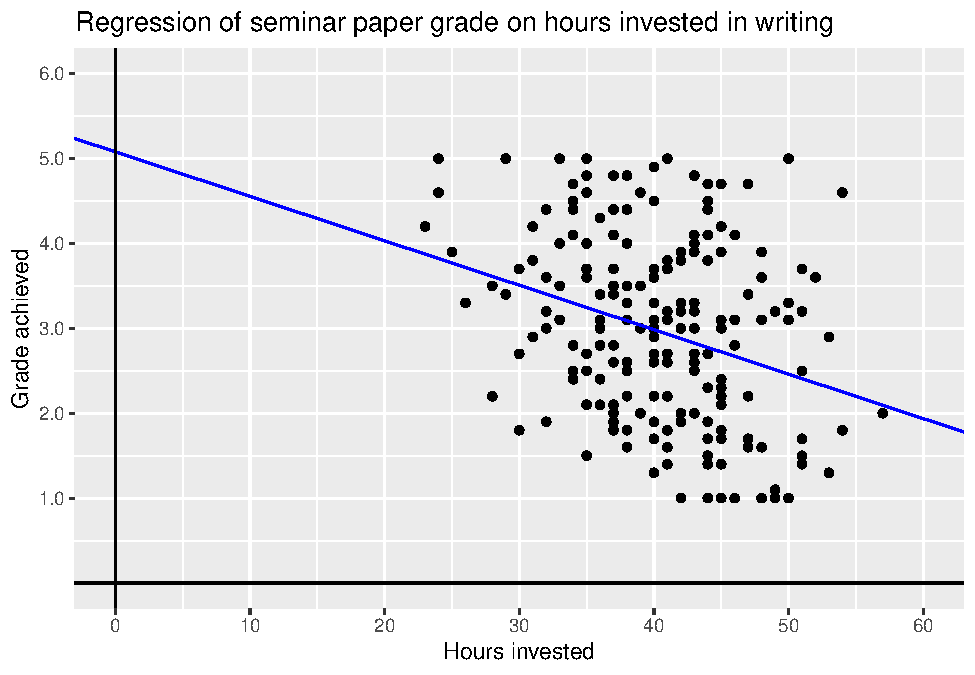
\includegraphics{_main_files/figure-latex/plot_lm_grade_hours-1.pdf}

What grade can a student expect, on average, if they invest exactly 0
hours, i.e.~do nothing and hand in a blank paper. We can look at the graph or,
to achieve a more precise result, calculate it.

\[5.07912 -0.05236 * 0 = 5.07912\]

For this theoretical example of \(x_{hours} = 0\), the estimated value \(\hat{y}\)
or \(y_{grade}\) is the same as the intercept \(\beta_0\). This is what the
intercept represents in general, the estimated value \(\hat{y}\) when the
dependent variable equals \(0\).

Investing zero hours in a seminar paper is not only not advisable, it is
also not a value we observed in our data. If the data would include observations
with zero hours of time invested, the grade would be a firm \(5.0\) and the same
would be true for low single digits, i.e.~turning in a two-pager as a seminar
paper. The takeaway is, that the model is highly dependent on the data that it
is trained on. If the data would have included such cases we could expect a
higher intercept and a steeper slope, i.e.~a stronger negative coefficient.

Luckily all our simulated students have put in at least some hours. But as we do
not have data for zero to \(22\) hours, we can not really make reliable estimates
in this range. Because of this, it does not really make sense to enter \texttt{hours}
into the regression model as ranging from \(0\) to \(57\). One solution that is
often used for metric variables is to center them on their mean. This can be
achieved by simply subtracting the mean of \(x\) from each individual value:

\[x_i - \bar{x}\]

We can now rerun the regression.

\begin{verbatim}
## 
## Call:
## lm(formula = grade ~ hours_centered, data = grades)
## 
## Residuals:
##      Min       1Q   Median       3Q      Max 
## -1.88006 -0.83961 -0.08006  0.77006  2.53881 
## 
## Coefficients:
##                Estimate Std. Error t value Pr(>|t|)    
## (Intercept)     2.96750    0.07267  40.835  < 2e-16 ***
## hours_centered -0.05236    0.01159  -4.517 1.07e-05 ***
## ---
## Signif. codes:  0 '***' 0.001 '**' 0.01 '*' 0.05 '.' 0.1 ' ' 1
## 
## Residual standard error: 1.028 on 198 degrees of freedom
## Multiple R-squared:  0.09344,    Adjusted R-squared:  0.08886 
## F-statistic: 20.41 on 1 and 198 DF,  p-value: 1.075e-05
\end{verbatim}

Comparing the results to the first model shows us, that the coefficient for
\(b_{hours\_centered}\) is exactly the same as for \(b_{hours}\). So the effect
of working more hours has not changed. What has changed is the value of the
intercept. This will make more sense if we again plot the regression line.

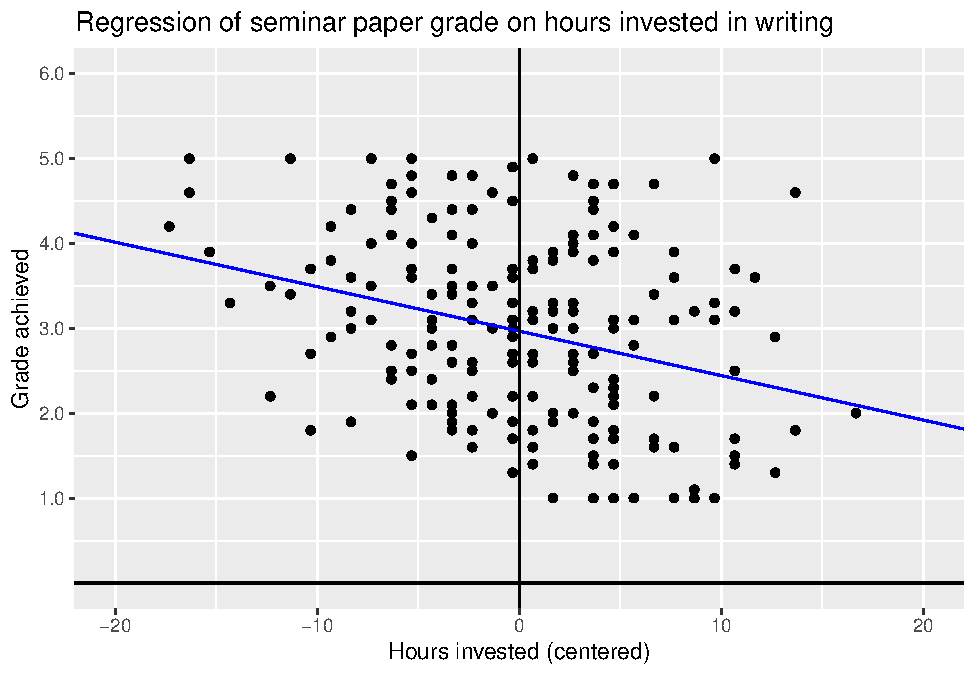
\includegraphics{_main_files/figure-latex/plot_lm_grade_hours_centered_0-1.pdf}

By centering the x-Variable on its mean we have changed its interpretation.
A value of \texttt{hours\ =\ 0} now stands for investing as much time as the mean
of \texttt{hours} in the whole data set, which in this case is \(40.33\) hours. Positive
values indicate that a student worked \(x\) hours more, negatives indicate \(-x\)
hours less compared to the mean. In this way, we also moved the y-axis and thus
changed the interpretation of the intercept. Its new value of \(2.9675\) now
indicates the estimate for a student who invests the mean value of \texttt{hours} in
their work, i.e.~\(40.33\).

\hypertarget{moving-on-1}{%
\section{Moving on}\label{moving-on-1}}

Based on our simple linear regression model we achieved an estimate for our
effect of interest. Working more hours results in receiving a better grade.
But there could be other variables that influence this relationship. In the
\protect\hyperlink{lin-t-2}{next session} we learn how we can include these in our model, when we move from
simple to multiple linear regression.

\hypertarget{lin-t-2}{%
\chapter{Linear Regression - Theory II: Multiple Linear Regression}\label{lin-t-2}}

Maybe explaining the grade a student receives solely based on the hours of
invested time does not paint the whole picture. As we have alluded to, there
may be other variables that could affect the relationship between \texttt{hours} and
\texttt{grade}.
If we fail to include these in our model, we may not get an unbiased estimate
for our effect of interest. Maybe the actual effect for \texttt{hours} is even stronger,
maybe it is weaker, or maybe there is no effect at all.
To assess this, we have to move from simple to multiple linear regression.

\hypertarget{objectives-3}{%
\section{Objectives}\label{objectives-3}}

\begin{itemize}
\tightlist
\item
  Expand the idea to multiple linear regression
\item
  Interpreting different types of independent variables
\item
  Understand measures of uncertainty
\end{itemize}

\hypertarget{multiple-linear-regression}{%
\section{Multiple Linear Regression}\label{multiple-linear-regression}}

A \emph{simple linear regression} only allows for one independent variable. This is
why we need \emph{multiple linear regression} if we want to start introducing
additional variables into the model. Luckily this is easy to understand as we
already know the formula for a simple linear regression:

\[y = \beta_0 + \beta_1*x_1 + \epsilon\]

To change a simple into a multiple linear regression, we just start adding the
additional variables and their coefficients additively to the formula.

\[y = \beta_0 + \beta_1*x_1 + \beta_2*x_2 + ... + \beta_k*x_k + \epsilon\]

So to add a second variable and its coefficient we add the term \(+ \beta_2*x_2\)
and so on until we added all independent variables of interest \(k\) to the model.
Everything else works exactly as for the simple model.

\hypertarget{adding-additional-metric-variables}{%
\subsection{Adding additional metric variables}\label{adding-additional-metric-variables}}

We already expected that the mean of the previous grades could be a strong
predictor for future grades. We could understand these as a \emph{proxy} variable for
the general skill level of a student. The higher the skill level, the higher
previous grades will have been.

How we can add additional variables in R code will again be a topic for the next
session, but let us look at the results of a regression of \texttt{grade} on
\texttt{hours\_centered} and \texttt{previous\_grades\_centered}, the latter being centered on the
mean previous grade of \(2.935\).

\begin{verbatim}
## 
## Call:
## lm(formula = grade ~ hours_centered + previous_grades_centered, 
##     data = grades)
## 
## Residuals:
##      Min       1Q   Median       3Q      Max 
## -1.44462 -0.30556  0.00622  0.32878  1.31002 
## 
## Coefficients:
##                           Estimate Std. Error t value Pr(>|t|)    
## (Intercept)               2.967500   0.038316  77.449   <2e-16 ***
## hours_centered           -0.056543   0.006114  -9.248   <2e-16 ***
## previous_grades_centered  0.904079   0.039830  22.699   <2e-16 ***
## ---
## Signif. codes:  0 '***' 0.001 '**' 0.01 '*' 0.05 '.' 0.1 ' ' 1
## 
## Residual standard error: 0.5419 on 197 degrees of freedom
## Multiple R-squared:  0.7492, Adjusted R-squared:  0.7467 
## F-statistic: 294.3 on 2 and 197 DF,  p-value: < 2.2e-16
\end{verbatim}

As we added a new variable, we now see three coefficients.
The intercept has not changed. It now indicates the estimated grade for a
student who invests the mean amount of hours, \(40.33\), and whose previous grades
are exactly \(2.935\), the mean of the variable.

The coefficient for \texttt{hours\_centered} got mildly more negative, still telling us
that the value of \texttt{grade} gets lower, the more hours are invested in writing the
paper. This coefficient now gives us the effect while \emph{controlling} for the
effect of \texttt{previous\_grades\_centered}. This is what multiple linear regression
does, giving us the coefficients for our variables of interest while keeping all
other independent variables at specific values. As we have centered the variable
for previous grades, the coefficient for \texttt{hours\ centered} gives us the effect
when the previous grades were exactly at the mean of \(2.935\).

In the same way, the coefficient for \texttt{previous\_grades\_centered} gives us the
effect of previous grades when the invested hours are controlled for, in this
case when the invested hours were exactly \(40.33\). The coefficient is rather
high and positive. This indicates that a student with a previous grade value
that is \(1\) above the mean, is estimated to receive a new grade that is \(0.9\)
points above the intercept. This means, that the previous grade is a very strong
predictor for the new grade.

While plotting in more than two dimensions gets really hard, we can still
calculate \(\hat{y}\) for certain values of both independent variables.
We already know the predicted grade for a student with mean values on both
independent variables, as this is the intercept. To make sure that we correct,
we can calculate it again.

\[b_0 + b_{hours\_centered}*0 + b_{previous\_grades\_centered}*0 = 2.9675\]

For this case we can see that the previous grade actually is a strong
predictor, as the previous and new grades are substantially the same.

What if a student whose previous grades were \(1\) above the mean, so just below
\(4.0\), but who decides to invest \(10\) hours more than the mean in writing the new paper?

\[2.9675 - 0.056543 * 10 + 0.904079 * 1 = 3.306149\]

So the good message is, while previous grades are a strong predictor, putting in
more hours still leads to better grades.

What if a really good student decides to rely on their skill and to work less
this time?

\[2.9675 - 0.056543 * -10 + 0.904079 * -2 = 1.724772\]

While \(1.7\) is still a very good grade, working 10 less hours than the mean of
students leads to a substantially worse estimate compared to the about \(1.0\)
received in previous grades.

\hypertarget{adding-dummy-variables}{%
\subsection{Adding dummy variables}\label{adding-dummy-variables}}

Another variable that could be of interest in explaining the received grade,
is if a student attended most of the seminar sessions.
\texttt{attendance} holds this information in the form of a dummy variable. Dummies can
only have two states. ``Yes'' or ``No'', ``1'' or ``0'' or in this case ``\texttt{TRUE}'' or
``\texttt{FALSE}''.

Let us add the variable to our model.

\begin{verbatim}
## 
## Call:
## lm(formula = grade ~ hours_centered + previous_grades_centered + 
##     attendance, data = grades)
## 
## Residuals:
##      Min       1Q   Median       3Q      Max 
## -1.41059 -0.30910  0.01667  0.35607  1.29849 
## 
## Coefficients:
##                           Estimate Std. Error t value Pr(>|t|)    
## (Intercept)               3.157411   0.078658  40.141  < 2e-16 ***
## hours_centered           -0.053942   0.006088  -8.860 4.85e-16 ***
## previous_grades_centered  0.911802   0.039282  23.212  < 2e-16 ***
## attendanceTRUE           -0.248250   0.090246  -2.751   0.0065 ** 
## ---
## Signif. codes:  0 '***' 0.001 '**' 0.01 '*' 0.05 '.' 0.1 ' ' 1
## 
## Residual standard error: 0.5331 on 196 degrees of freedom
## Multiple R-squared:  0.7586, Adjusted R-squared:  0.7549 
## F-statistic: 205.3 on 3 and 196 DF,  p-value: < 2.2e-16
\end{verbatim}

This gives us a new line in the R Output holding an estimate for
\texttt{attendanceTRUE}. What is meant by this? In contrast to the metric variables we
have uses in our model up to this point, a dummy variable - or binary variable -
can only have two states. As we are using a logical variable here, it can only
have the value \texttt{TRUE} - here indicating regular attendance - or \texttt{FALSE}. So what
the output shows us, is the effect of attendance being \texttt{TRUE} compared to being
\texttt{FALSE}. If a student did regularly attend the seminar, the estimated grade is
\(-0.248250\) lower compared to when they did not.

We can observe what happens in the formula:

\[\hat{y} = b_0 + b_{hours\_centered}*x_{hours\_centered} + \\
b_{previous\_grades\_centered} * x_{previous\_grades\_centered} +\\ 
b_{attendance} * x_{attendance}\]

If you calculate with \texttt{TRUE} and \texttt{FALSE} in R, the values \(1\) and \(0\) are used
respectively. So \(x_{attendance}\) can either have the value \(1\) for regular
attendance or \(0\) for not so regular attendance.

If a student did regularly attend, the coefficient \$b\_\{attendance\} becomes a
part of the estimate \(\hat{y}\):

\[\hat{y} = b_0 + b_{hours\_centered}*x_{hours\_centered} +\\
b_{previous\_grades\_centered}*x_{previous\_grades\_centered} +\\ 
b_{attendance} * 1\]

If student did not regularly attended, this happens:

\[\hat{y} = b_0 + b_{hours\_centered}*x_{hours\_centered} \\
+ b_{previous\_grades\_centered}*x_{previous\_grades\_centered} +\\
b_{attendance} * 0\]

Which shortens to:

\[\hat{y} = b_0 + b_{hours\_centered}*x_{hours\_centered} +\\
b_{previous\_grades\_centered}*x_{previous\_grades\_centered}\]

The coefficient is no longer a part of the estimate. One can basically say, the
coefficient gets switched on or off by the value of the dummy variable.

So while the estimate for a student with mean values for invested hours and
previous grades who did not attend is equal to the intercept of \(3.157411\),
for a similar student who attended we can calculate the estimate as:

\[3.157411 - 0.053942*0 + 0.911802*0 - 0.248250 * 1 = 3.157411 - 0.248250 \\
= 2.909161\]

It seems attending class is an easy way to raise one's grades.

\hypertarget{adding-categorical-variables}{%
\subsection{Adding categorical variables}\label{adding-categorical-variables}}

We have one further variable in our simulated data set that could be of interest
in explaining, what makes a good grade in a seminar paper. \texttt{contact} is a
categorical variable, or a factor variable in R terms.
It can take three different categories. \texttt{No\ contact} indicates that
the student did not contact the lecturer to discuss a research question or the
laid out plan for the paper. \texttt{E-Mail} means that there was some written contact
and at least the basics for the paper were discussed before writing. Lastly,
\texttt{In\ Person} stands for an in depth discussion with the lecturer, clearing up
problems beforehand and thus potentially having a more stringent vision for the
paper before writing the first word.

Let us add the variable to our model.

\begin{verbatim}
## 
## Call:
## lm(formula = grade ~ hours_centered + previous_grades_centered + 
##     attendance + contact, data = grades)
## 
## Residuals:
##     Min      1Q  Median      3Q     Max 
## -1.3835 -0.2525  0.0167  0.2678  0.9347 
## 
## Coefficients:
##                           Estimate Std. Error t value Pr(>|t|)    
## (Intercept)               3.617949   0.068077  53.145  < 2e-16 ***
## hours_centered           -0.050830   0.004433 -11.466  < 2e-16 ***
## previous_grades_centered  0.874123   0.028657  30.503  < 2e-16 ***
## attendanceTRUE           -0.324653   0.065781  -4.935 1.72e-06 ***
## contactE-Mail            -0.413808   0.069817  -5.927 1.39e-08 ***
## contactIn Person         -0.853252   0.063964 -13.340  < 2e-16 ***
## ---
## Signif. codes:  0 '***' 0.001 '**' 0.01 '*' 0.05 '.' 0.1 ' ' 1
## 
## Residual standard error: 0.3869 on 194 degrees of freedom
## Multiple R-squared:  0.8741, Adjusted R-squared:  0.8709 
## F-statistic: 269.4 on 5 and 194 DF,  p-value: < 2.2e-16
\end{verbatim}

Wait, we entered three categories into the model and got estimates for two of
them. What happened? What R does is to create two dummy variables on the fly.
The first discerns between having E-Mail contact and no contact at all. The
second one between having contact in person and no contact at all. So for
categorical variables in regression models we always compare being in one of the
categories to being in the \emph{base category}. In this case the base category is
\texttt{No\ contact}, but we could also change the base category. It depends on what we
are interested in comparing to. For our example comparing the effects of having
more in depth contact to having none makes sense.

Let us look at our formula again:

\[\hat{y} = b_0 + b_{hours\_centered}*x_{hours\_centered} +\\
b_{previous\_grades\_centered} * x_{previous\_grades\_centeerd} +\\
b_{attendance} * x_{attendance} +\\
b_{E-Mail} * x_{E-Mail} + b_{In Person} * x_{In Person}\]

Now there are three possibilities. A student can have no contact at all. In this
case both dummy variables are equal to \(0\). To make our formula easier to read, we have
abbreviated the middle part for now:

\[\hat{y} = b_0 + ... + b_{E-Mail} * 0 + b_{In Person} * 0\]

So in this case controlling all other independent variables at their default
values, the mean for the metric variables and \texttt{FALSE} for \texttt{attendance}, the
intercept gives us the estimate for the grade when the student had no contact to
the lecturer, as both dummy variables that were created for \texttt{contact} are ``switched off''.

The two other possibilities are that a student either had E-Mail contact or an
in person discussion:

\[\hat{y} = b_0 + ... + b_{E-Mail} * 1 + b_{In Person} * 0\]

\[\hat{y} = b_0 + ... + b_{E-Mail} * 0 + b_{In Person} * 1\]

In both cases the relevant dummy variable is ``switched on'' while the other does
not factor into the equation.

Looking at the estimates we can see that having contact to the lecturer before
writing has strong negative effects, resulting in better grades. Having E-Mail
contact reduces the value of \texttt{grade} by \(-0.413808\) points, having an in person
discussion by \(-0.853252\).

So what grade can a student whose previous grades were at the mean of \(2.935\),
but who decided to put in 20 hours more compared to their peers, regularly
attend the seminar and have an in-depth personal discussion before writing their
paper expect on average as their new grade?

\[3.617949 - 0.050830 * 20 + 0.874123 * 0 - 0.324653 * 1 - 0.413808 * 0 - 0.853252 * 1 
\\ = 1.423444\]

Putting in the hours, attending and working with your lecturer seems to pay off,
at least in our simulated data set.

\hypertarget{returning-to-our-research-question}{%
\section{Returning to our research question}\label{returning-to-our-research-question}}

Our exemplary research question concerned itself with what makes a good grade in
a seminar paper. In particular we were interested in the effect of the invested
hours, as our main hypothesis was that more hours lead to better grades. What do
we know now?

Our analysis points towards a clear effect from \texttt{hours} on \texttt{grade}. This effect
was consistently visible in all of our models. But did we correctly identify
and estimate the effect of interest? Maybe. The problem is, we actually did not
approach the analysis correctly. In a real analysis we should \textbf{absolutely}
refrain from adding variables to our model that \emph{could be} relevant until we are
satisfied or even until all available variables are bunched into one huge model.
It was fine to do this in this introduction to linear regression to learn how
different types of variables can be used in a regression model. But in a real
project, we have to invest time to think about which variables to add because we
assume that they have a relevant effect based on theoretical assumptions about
the processes we are interested in.

So let us do this now and vow do make this our first step in all future
endeavors. While we do not have a clear theoretical basis, we can make clear
assumptions on the data generating process and draw these in a DAG.

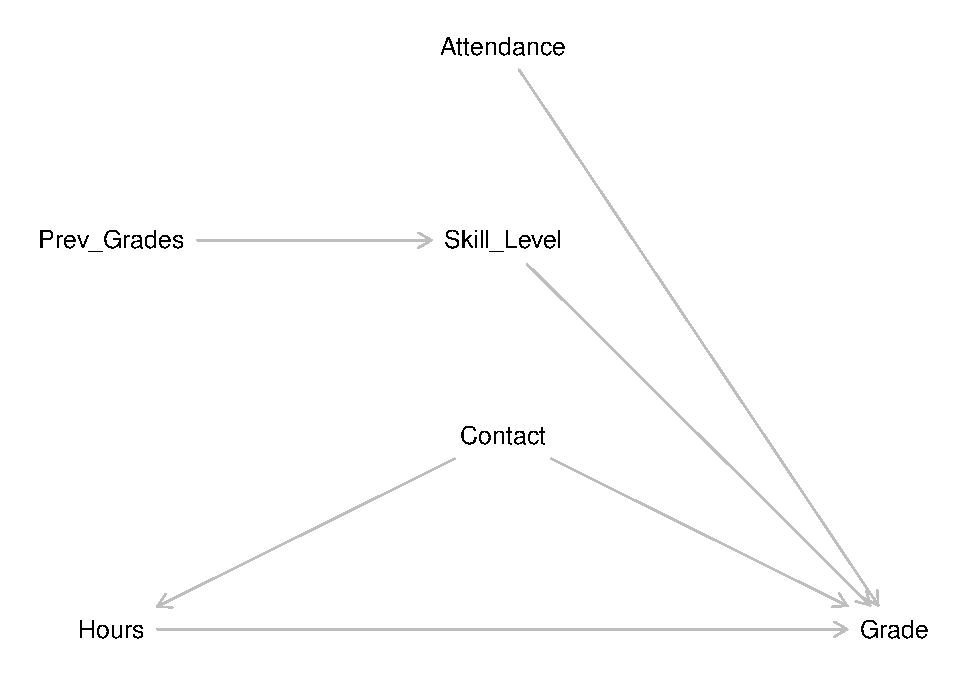
\includegraphics{_main_files/figure-latex/dag-1.pdf}

Our central assumption, and the effect we want to identify and estimate, is the
direct effect from \texttt{hours} on \texttt{grade} in the bottom line. The more hours a
student invests, the better the grade should be.

The assumed effect of \texttt{contact} is more complex. For one we assume that a more
in-depth contact with the lecturer will increase the grade directly. The
research question will be more focused, the student will know what is important
to a certain lecturer, common mistakes can be avoided if they are cleared up
beforehand and so on. But we will also assume that \texttt{contact} will have an effect
on \texttt{hours} in the sense that the hours invested can be used more efficiently if
an in-depth discussion has taken place. Instead of wasting time running into
problems that could have been avoided most of the invested time can actually go
into constructive work. This makes \texttt{contact} a confounder for \texttt{grade} and
\texttt{hours}.

A student's skill level will also have a direct effect on \texttt{grade}. As we do not
have a direct measure of skill in our data, we use \texttt{previous\_grades} as a proxy
for skill level. \texttt{attendance} is also assumed to have a direct effect on \texttt{grade}
as students who were present in the seminar will not only have learned the seminar's
contents, but will also have a better understanding of what is expected in their
seminar papers.

Tapping into the knowledge from session 4, we can now make implications for our
model from the DAG. Let us list all paths from \texttt{hours} to \texttt{grade}:

\[A: Hours \rightarrow Grade\]

\[B: Hours \leftarrow Contact \rightarrow Grade\]

Path A represents our effect of interest. On path B, \texttt{contact} is a confounder
for \texttt{hours} and \texttt{grade}. To close this path, we have to control for \texttt{contact}.
As neither skill level - or \texttt{previous\_grades} - nor \texttt{attendance} lie on a path
from our independent variable of interest to our dependent variable, we should
not control for them in our model.
That leaves us with \texttt{hours} and \texttt{contact} to be included in our linear
regression, if our goal is to get an unbiased estimate for the effect of
invested time on the final grade. So let us do this:

\begin{verbatim}
## 
## Call:
## lm(formula = grade ~ hours_centered + contact, data = grades)
## 
## Residuals:
##      Min       1Q   Median       3Q      Max 
## -1.85595 -0.74624 -0.02106  0.66648  2.50161 
## 
## Coefficients:
##                  Estimate Std. Error t value Pr(>|t|)    
## (Intercept)       3.44352    0.10404  33.098  < 2e-16 ***
## hours_centered   -0.04967    0.01052  -4.723 4.43e-06 ***
## contactE-Mail    -0.46482    0.16785  -2.769  0.00616 ** 
## contactIn Person -1.02804    0.15240  -6.746 1.67e-10 ***
## ---
## Signif. codes:  0 '***' 0.001 '**' 0.01 '*' 0.05 '.' 0.1 ' ' 1
## 
## Residual standard error: 0.9305 on 196 degrees of freedom
## Multiple R-squared:  0.2643, Adjusted R-squared:  0.253 
## F-statistic: 23.47 on 3 and 196 DF,  p-value: 5.072e-13
\end{verbatim}

This is our estimate. Each hour invested beyond the mean of \(40.33\) hours
changes the grade by about \(-0.05\) points. This supports our hypotheses and we
can conclude, that investing more hours into writing a seminar paper actually
is a worthwhile investment.

But remember: This is correct as long as our DAG is drawn correctly, which is
always debatable. Maybe we should assume an effect from skill level on \texttt{hours}.
The higher the skill level the more efficiently the available time can be used.
For this example we know the DAG is correct, because we have simulated the data
exactly in this way. For real world applications we never know if our DAG is
correct. All we can and \emph{have to} do is base it on thorough thinking,
theoretical work, exploratory data analysis and sound arguments.

This all is true \emph{if} our goal is to estimate an effect of interest as precisely
as possible. But as we have alluded to in the introduction to this session we
could also use modelling with a different goal, i.e.~predicting a grade as
accurately as possible. For this task, the model which only includes \texttt{hours} and
\texttt{contact} will not do the best job. From our DAG we know that \texttt{attendance} and
\texttt{previous\_grade} should have an effect on \texttt{grade}, as we have also seen in our
models. For this task the full model including all these variables will produce
better estimates. We will return to this in a later session, but for now we
should remember that we have to know our task because the task dictates which is
the best model to use.

\hypertarget{adressing-the-uncertainty}{%
\section{Adressing the uncertainty}\label{adressing-the-uncertainty}}

Looking at the coefficient block from the output, we see more
than just our estimates. The \texttt{Std.\ Error} - \emph{standard error} - is a measure for the
uncertainty of our estimates. It basically tells us, how far away the actual
values of the observations used to compute the model are from our estimate
\emph{on average}. The smaller the \emph{standard error}, the more accurate our
estimate. The standard error is presented in the units of the estimate and we
can thus compare them. A large standard error for a large estimate is far less
problematic compared to a large standard error for a small estimate.

The estimate and it's standard error are the basis for \emph{hypothesis testing}.
What we are testing is the \emph{alternative hypotheses} \(H_a\) that there actually
is an effect of our independent variable on the dependent variable against the
\emph{null hypothesis} \(H_0\) that there is no effect. To reject the null hypothesis
and be confident that we are observing an actual effect, versus an effect that
is just based on random variation in our sample, the estimate has to be far
away enough from \(0\) and be accurate enough, i.e.~have a small standard error.
This relationship is computed in the \emph{t-statistic}, \texttt{t\ value} in
our output. From this the \emph{p-value} can be computed, \texttt{Pr(\textgreater{}\textbar{}t\textbar{})} in the output.
The \emph{p-value} tells us the probability to observe an association
between the independent and the dependent variable as large or larger than our
estimate suggests, if the true association would actually be \(0\). If the p-value
is small enough, we can reject \(H_0\) and conclude that we observed an actual
effect. There are certain agreed upon cutoffs in statistics, while values that
meet this cutoffs are considered \emph{statistically significant}. The most common
cutoff in social sciences is \(0.05\) indicated by one \texttt{*} in the output.
Other common cutoffs are indicated by more asterisks. It is important to note,
that we can not say that more \texttt{*} behind an effect mean that this effect has a
higher statistical significance. We have to decide on a level of statistical
significance that we want to test for before we see the results. If we decide on
testing for a significance level of \(5\%\), seeing more than one star then only
means that the effect is also statistically significant at the \(5\%\) level.

Interpreting p-values correctly and not falling into the common pitfalls like the
one mentioned above is a
topic on its own. We do not have the time to dive into this here, so for now we
can agree that p-values below \(0.05\) indicate that we can reject \(H_0\) and thus
conclude that we have actually observed an effect. Still, our interpretation of
regression results should not focus solely on p-values or lead us to disregard
any effects that did not meet the cutoff. For example, we can have very small
p-values for effects that are so small that they are substantially irrelevant.
One way to address this is to inspect the actual magnitudes of the effects.
On the other hand, we
can have p-values larger than \(0.05\) for effects that are still relevant. Maybe
the problem is not that there is no effect but that we were not able to measure
the variable in question precisely enough or that we just did not have enough
observations. We can not go any deeper than this here, but we should remember
that the practice of declaring every effect with stars a win, or even with more
stars a bigger win, and disregarding
everything without them may still be common but is not the way to go forward.

In our model, we can see that the effect of interest is statistically
significant. We can thus conclude, that we have observed an actual effect
from \texttt{hours} on \texttt{grade}. Our estimate is large enough and our standard error
small enough to reach this conclusion.

\hypertarget{moving-on-2}{%
\section{Moving on}\label{moving-on-2}}

We have attained an estimate for our effect of interest which supports our
hypotheses that investing more hours into writing a paper leads to better grades.
So can we wrap a bow on the question and move on to finally figuring out what
is going on in our NBA data? Almost, but not yet. We still do not know, if our
model actually works as intended. Linear regression, as well as every other modelling
technique, has some underlying statistical assumptions that we have to meet for the model
to accurately estimate an effect. In the \protect\hyperlink{lin-t-3}{next session} we will get to know these
assumptions and how we can test for them.

\hypertarget{lin-t-3}{%
\chapter{Linear Regression - Theory III: Diagnostics}\label{lin-t-3}}

In this session we will get to know the central underlying assumptions for linear regression models. To find out if our model actually works as intended and thus gives us a reliable estimate for the effect of \texttt{hours} on \texttt{grade}, we have to check if we have met these assumptions, and if we did not, we have to correct our model accordingly. Before we do this, we should briefly consider another part of the regression output, the model fit.

\hypertarget{objectives-4}{%
\section{Objectives}\label{objectives-4}}

\begin{itemize}
\tightlist
\item
  Learn about model fit and its limits
\item
  Understand the statistical assumptions underlying linear regression
\item
  Test for violated assumptions and learn how to correct for those
\end{itemize}

\hypertarget{model-fit}{%
\section{Model fit}\label{model-fit}}

Let us again inspect the output from the simplest model we computed, regressing the grade solely on the invested hours:

\begin{verbatim}
## 
## Call:
## lm(formula = grade ~ hours_centered, data = grades)
## 
## Residuals:
##      Min       1Q   Median       3Q      Max 
## -1.88006 -0.83961 -0.08006  0.77006  2.53881 
## 
## Coefficients:
##                Estimate Std. Error t value Pr(>|t|)    
## (Intercept)     2.96750    0.07267  40.835  < 2e-16 ***
## hours_centered -0.05236    0.01159  -4.517 1.07e-05 ***
## ---
## Signif. codes:  0 '***' 0.001 '**' 0.01 '*' 0.05 '.' 0.1 ' ' 1
## 
## Residual standard error: 1.028 on 198 degrees of freedom
## Multiple R-squared:  0.09344,    Adjusted R-squared:  0.08886 
## F-statistic: 20.41 on 1 and 198 DF,  p-value: 1.075e-05
\end{verbatim}

Up to now, we exclusively talked about the coefficient block. We will return to the ``Call'' \protect\hyperlink{lin-a}{next session} and to the ``Residuals'' later in this session. For now let us focus on the bottom block in the output.

\(R^2\) or \emph{R-squared} is a measure for the amount of variance in the data that is ``explained'' by the model. Real world data will always have variance. Not every value will neatly fall onto the mean value of a variable. Rather the data is dispersed around it. The same is true for our dependent variable:

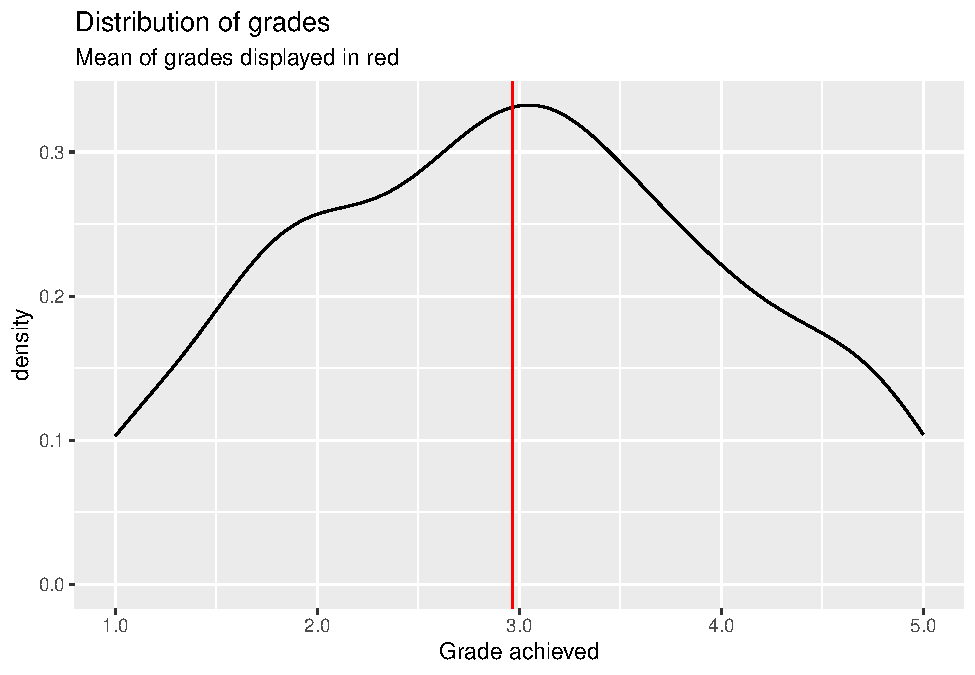
\includegraphics{_main_files/figure-latex/plot_grade_distribution-1.pdf}

This is a density plot and shows the distribution of a metric variable as a smoothed line. We do not see every individual actual value but the general shape of the data. The red line represent the mean of \texttt{grade}, which is about \(2.97\). Most actual values are not exactly at the mean but are rather dispersed around it, ranging between \(1.0\) and \(5.0\). This is the variance in our outcome variable.

Let us now plot \texttt{grade} against \texttt{hours\_centered} and add the regression line from our model above:

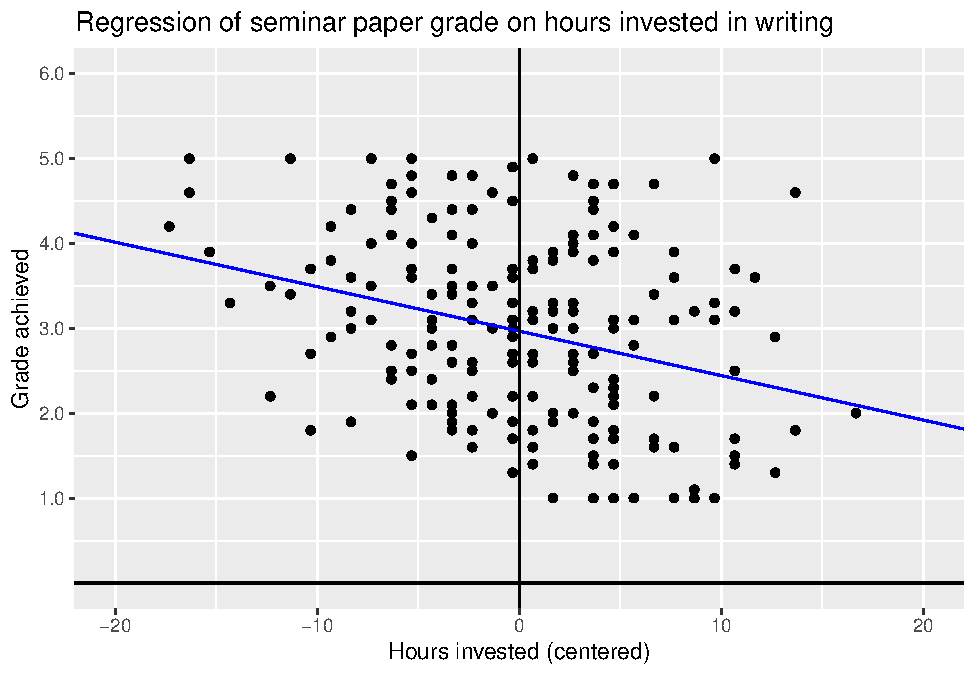
\includegraphics{_main_files/figure-latex/plot_lm_grade_hours_centered-1.pdf}

Without our regression line, all we would have is a cloud of points without much order to it. What linear regression does, is trying to bring order into this by fitting a line that best explains the variance of the dependent variable, \texttt{grade} in our case by its relationship to one or multiple dependent variables, here \texttt{hours\_centered}. But this linear line can never explain the variance completely. For this it had to pass through every data point. Our line does not. Actually most data points do not lie on the regression line but at some distance to it. You will remember that OLS computes \emph{the} regression line for which the squared distances are smallest. This is the line that explains most of the variance of \(y\) by its relationship to \(x\), but not all variance is explained. An unexplained part remains. These are the residuals; the distance that points fall from the regression line. \(R^2\) tells us the relative amount of how much we reduced the initial variance by fitting the line and thus explaining a part of said variance.

A \(R^2\) of \(0\) would mean that no variance is explained, a value of \(1\) that all variance is explained. Two highly unlikely outcomes. We will almost always explain something and never explain everything.

In our model \(R^2\) equals \(0.09344\). This means we explained about \(9.3\%\) of the variance of \texttt{grade} by its relationship with \texttt{hours\_centered}. That's nice, but this also means that over \(90\%\) are still unexplained. We will not explain all of the variance, i.e.~\(R^2 = 1\), but in general a higher \(R^2\) is desirable.

So what can we do? We can try to add additional variables to the model that help in explaining the variance of the outcome variable. Last session we concluded that the best model to measure the effect of invested hours on the achieved grade would also have to include \texttt{contact}:

\begin{verbatim}
## 
## Call:
## lm(formula = grade ~ hours_centered + contact, data = grades)
## 
## Residuals:
##      Min       1Q   Median       3Q      Max 
## -1.85595 -0.74624 -0.02106  0.66648  2.50161 
## 
## Coefficients:
##                  Estimate Std. Error t value Pr(>|t|)    
## (Intercept)       3.44352    0.10404  33.098  < 2e-16 ***
## hours_centered   -0.04967    0.01052  -4.723 4.43e-06 ***
## contactE-Mail    -0.46482    0.16785  -2.769  0.00616 ** 
## contactIn Person -1.02804    0.15240  -6.746 1.67e-10 ***
## ---
## Signif. codes:  0 '***' 0.001 '**' 0.01 '*' 0.05 '.' 0.1 ' ' 1
## 
## Residual standard error: 0.9305 on 196 degrees of freedom
## Multiple R-squared:  0.2643, Adjusted R-squared:  0.253 
## F-statistic: 23.47 on 3 and 196 DF,  p-value: 5.072e-13
\end{verbatim}

We can use \(R^2\) to compare the \emph{model fit} of multiple models. Here the larger model achieved a considerably higher value of \(R^2 = 0.2643\). The model fit improved as we can now explain a higher ratio of the variance in \texttt{grade}.

After \(R^2\) we see another value, \emph{Adjusted R-squared}. This becomes relevant if we add additional variables to our model. \(R^2\) almost always increases, and never decreases, when adding additional variables to the model, especially if we have few observations. Because of this \(R^2\) can get less reliable when we have many variables and few observations. \emph{Adjusted R-squared} corrects for this by including both factors in the calculation. When we have many observations the differences are negligible. This is true for our case. We have relatively many observations and few variables in our model, so the values of both measures are rather close. But in cases where this relationship is not as favorable, adjusted R-squared should be used in place of the regular \(R^2\).

The block in our output also gives us the \emph{Residual standard error}. As we have seen above, most actual data point do not lie on the regression line but some distance away from it. These are the residuals. Thus their standard error basically tells us how much we miss the spot on average. As it is given in units of the dependent variable, we can say that the estimates for \texttt{grade} based on our second model are on average \(0.93\) off. A considerable amount, as this is almost one whole grading step. This is still an improvement from the \(1.028\) in the first model but nevertheless a substantial error.

The last line in the output gives us two connected measures. The \emph{F-statistic} is the test statistic for \(R^2\) and is used the compute the corresponding \emph{p-value}. In this case we are testing if the \(R^2\) our model returned based on our sample is possible, when the actual population value of \(R^2\) is \(0\). In other words, could we have achieved this \(R^2\) by chance if the independent variables in our model actually do not explain part of the variance in the population? Both of our models have very small p-values, so it is highly unlikely that we have just explained some variance by chance. This gives further credibility to our model specification.

We can conclude that the second model was an improvement over the first. But can we do more? Sure; we can always add additional explanatory variables:

\begin{verbatim}
## 
## Call:
## lm(formula = grade ~ hours_centered + previous_grades_centered + 
##     attendance + contact, data = grades)
## 
## Residuals:
##     Min      1Q  Median      3Q     Max 
## -1.3835 -0.2525  0.0167  0.2678  0.9347 
## 
## Coefficients:
##                           Estimate Std. Error t value Pr(>|t|)    
## (Intercept)               3.617949   0.068077  53.145  < 2e-16 ***
## hours_centered           -0.050830   0.004433 -11.466  < 2e-16 ***
## previous_grades_centered  0.874123   0.028657  30.503  < 2e-16 ***
## attendanceTRUE           -0.324653   0.065781  -4.935 1.72e-06 ***
## contactE-Mail            -0.413808   0.069817  -5.927 1.39e-08 ***
## contactIn Person         -0.853252   0.063964 -13.340  < 2e-16 ***
## ---
## Signif. codes:  0 '***' 0.001 '**' 0.01 '*' 0.05 '.' 0.1 ' ' 1
## 
## Residual standard error: 0.3869 on 194 degrees of freedom
## Multiple R-squared:  0.8741, Adjusted R-squared:  0.8709 
## F-statistic: 269.4 on 5 and 194 DF,  p-value: < 2.2e-16
\end{verbatim}

The p-value is even lower, and the F-statistic even higher, compared to our second model, but this was never an issue. What is more interesting is that we have substantially increased \(R^2\) and decreased the residual standard error. As we have concluded last week, this larger model is better at predicting the actual values of \texttt{grade}. Thus the explained variance has to increase and the average error in estimating \texttt{y} has to decrease. But is this the better model? The values on the model fit would suggest so. And this also is true, if our aim is predicting \texttt{grade} to the best of our abilities. But if our aim is still measuring the effect of \texttt{hours} on \texttt{grade} we know from our DAG that we do not have to or even should not control for the additional variables to get an unbiased estimator for the effect of interest.

What can we take away from this? While the model fit measures are an important tool for comparing multiple possible models and better values are desirable in general, it should not be our goal to just max out all measures and declare this model the ``winner''. It is never that easy in statistics. One thing we can never replace is thorough theoretical work before even computing our first model. Based on our DAG, if it is correct, we know that we do not have to control for previous grades and attendance. Including them may give us a larger \(R^2\), but is still not the correct way to build our model.

Based on this our best model is still the second one:

\begin{Shaded}
\begin{Highlighting}[]
\FunctionTok{summary}\NormalTok{(m2)}
\end{Highlighting}
\end{Shaded}

\begin{verbatim}
## 
## Call:
## lm(formula = grade ~ hours_centered + contact, data = grades)
## 
## Residuals:
##      Min       1Q   Median       3Q      Max 
## -1.85595 -0.74624 -0.02106  0.66648  2.50161 
## 
## Coefficients:
##                  Estimate Std. Error t value Pr(>|t|)    
## (Intercept)       3.44352    0.10404  33.098  < 2e-16 ***
## hours_centered   -0.04967    0.01052  -4.723 4.43e-06 ***
## contactE-Mail    -0.46482    0.16785  -2.769  0.00616 ** 
## contactIn Person -1.02804    0.15240  -6.746 1.67e-10 ***
## ---
## Signif. codes:  0 '***' 0.001 '**' 0.01 '*' 0.05 '.' 0.1 ' ' 1
## 
## Residual standard error: 0.9305 on 196 degrees of freedom
## Multiple R-squared:  0.2643, Adjusted R-squared:  0.253 
## F-statistic: 23.47 on 3 and 196 DF,  p-value: 5.072e-13
\end{verbatim}

\hypertarget{regression-diagnostics}{%
\section{Regression diagnostics}\label{regression-diagnostics}}

As linear regression is a statistical technique, there are certain statistical assumptions we have to meet. If we violate those, the best laid plans may falter and our results may be not as robust as we hoped. Let us go through these assumptions and the tests to check for them one by one.

\hypertarget{linearity}{%
\subsection{Linearity}\label{linearity}}

The name already gives it away, a \emph{linear} regression is used to estimate \textbf{linear} relationships between variables. For this to work, the relationships actually have to be linear. But a relationship between two variables can have other functional forms. Consider this for example:

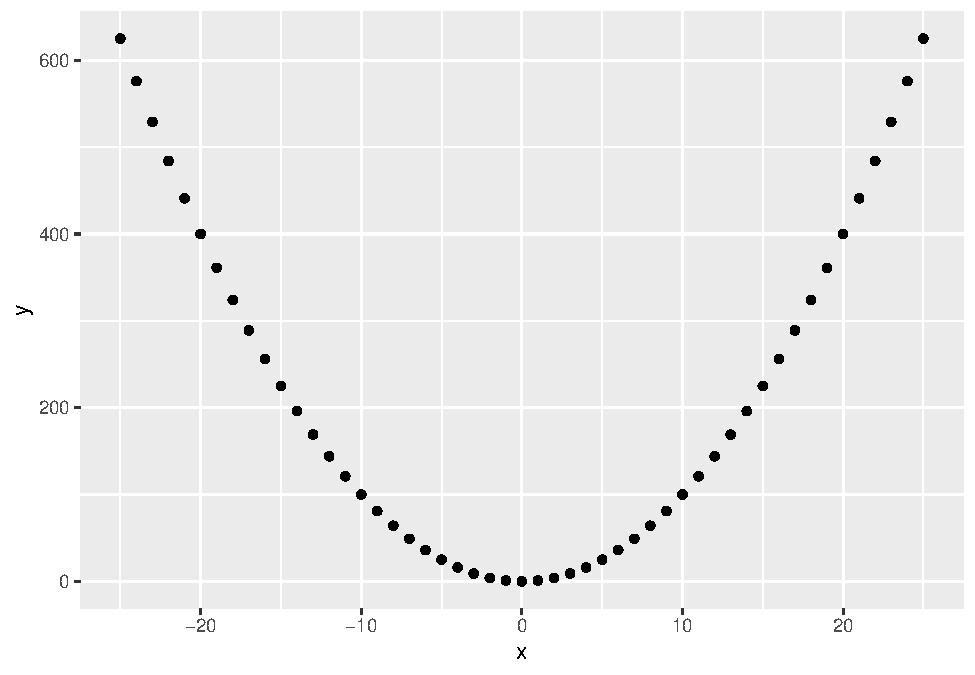
\includegraphics{_main_files/figure-latex/non_linear-1.pdf}

The relationship is clearly not linear. But we can still fit a regression and get a result:

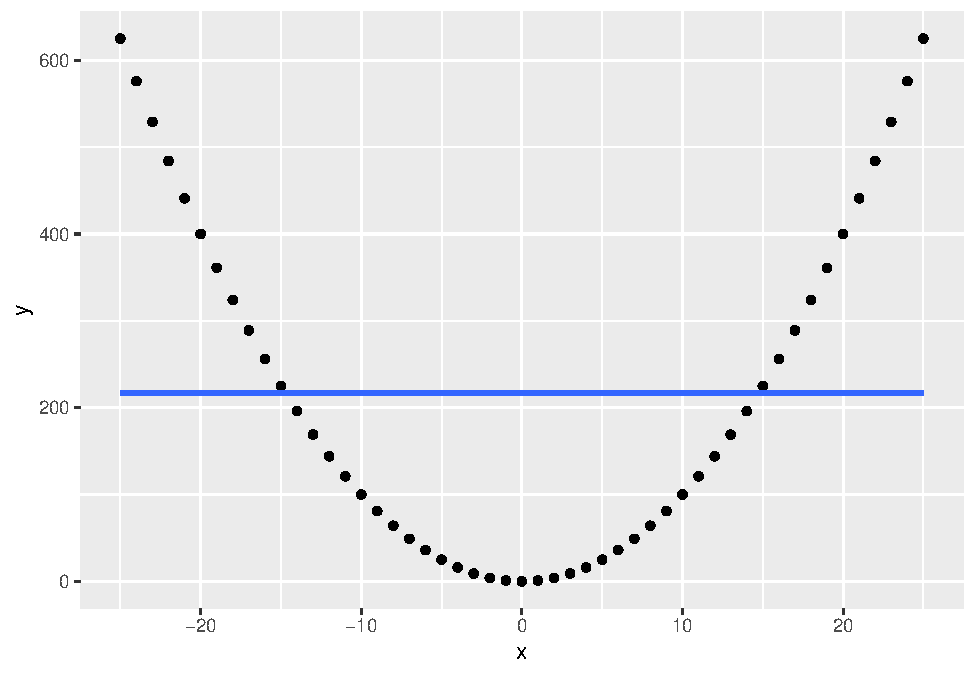
\includegraphics{_main_files/figure-latex/non_linear_reg-1.pdf}

The regression line shows us that \texttt{x} and \texttt{y} are completely uncorrelated. This is clearly not true, but as our linear regression assumes linearity, it tries to model the relationship in linear terms.

What we can do in such cases is to transform the variable in question in a non-linear way. Here the quadratic relationship is easy to spot, so if we transform \(x\) to \(x^2\), this happens:

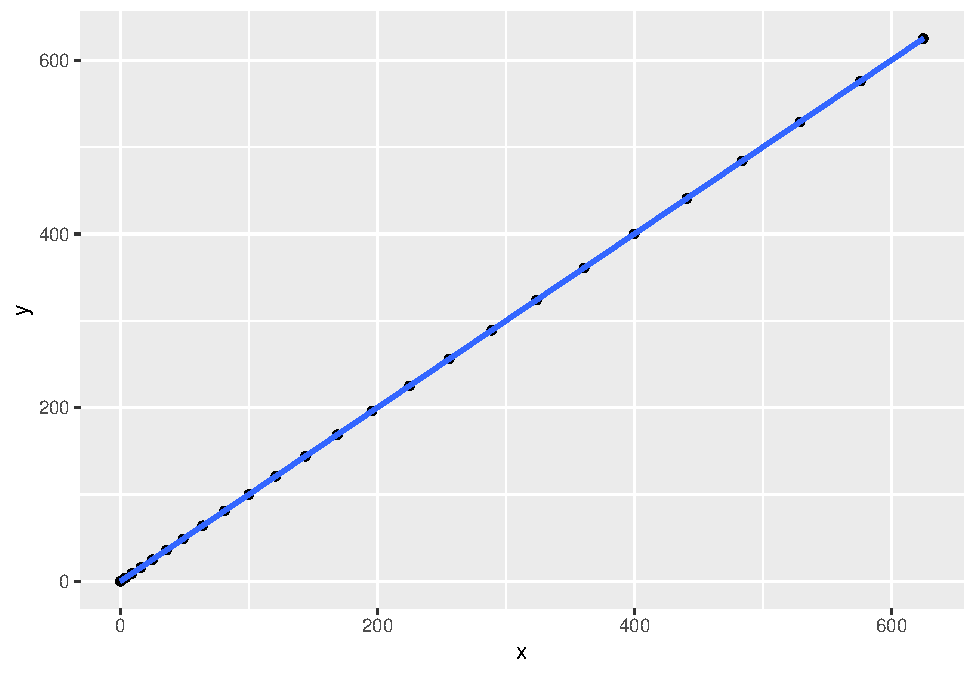
\includegraphics{_main_files/figure-latex/non_linear_reg_squared-1.pdf}

The non-linear relationship between \texttt{x} and \texttt{y} has been transformed into a linear one.

For real world data, the non-linearity most often is not as straightforward to spot as in this example. A first step to approach this, is inspecting a scatterplot matrix. This is usually done before starting to model to identify relationships between the variables used.

\begin{verbatim}
## Warning: package 'GGally' was built under R version 4.2.3
\end{verbatim}

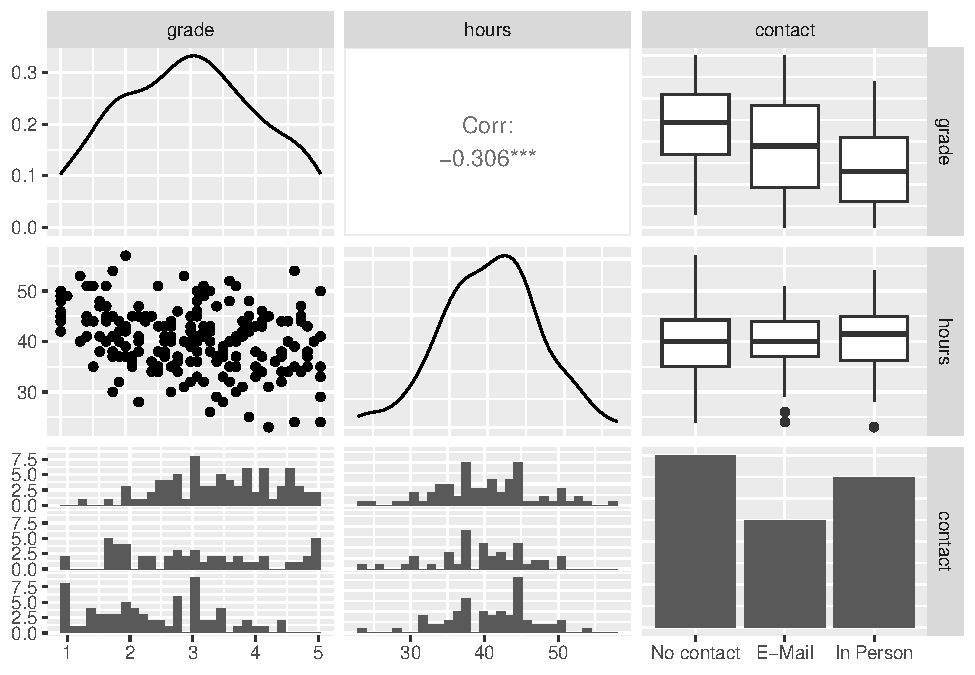
\includegraphics{_main_files/figure-latex/scatterplot_matrix-1.pdf}

The diagonal displays the distribution of all variables included. Here metric variables are displayed as density plots and categorical variables as bar plots. Below and above the diagonal the relationship between two variables is shown. The scatterplot on the left of the second row is the one between \texttt{hours} and \texttt{grade} we have already seen several times. There is no indication of non-linearity here. What we have not inspected yet, is the relationship between \texttt{contact} and the two other variables.

The bottom row contains histograms of the two metric variables by the category of contact, the right column boxplots for the same combination. Without going into too much detail on both types of plots, both show us how the distribution for both metric variables changes by category. The more personal the contact with the lecturer, the lower the center of the distribution of final grades is. This makes sense, as we have already seen this correlation in the results of our model. Between \texttt{hours} and \texttt{contact} there seems to be no correlation. The amount of hours a student invests in writing the paper, does not lower the hours invested in a systematic way.

But this does not clear the model of suspicions of non-linearity just yet. Even when all pairwise relationships are linear, controlling for multiple variables at the same time can introduce non-linearity for this specific combination. One way to approach this is to inspect the \emph{Residuals vs.~Fitted} plot. As the name suggests, this plots the fitted values, i.e.~the estimates for our dependent variables based on the model, against the residuals of the dependent variable. When the relationship is linear, we should see a more or less straight line along the x-axis, where \(y = 0\).

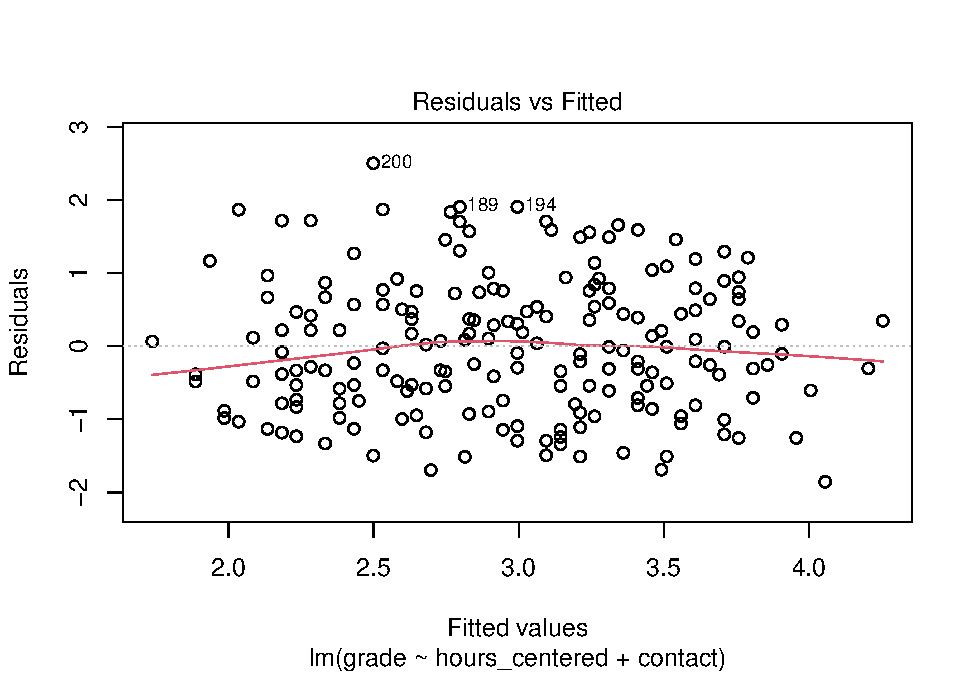
\includegraphics{_main_files/figure-latex/residuals_fitted-1.pdf}

For many use cases, the line is straight enough, indicating no clear and strong patterns of non-linearity. Still the residuals seem to be slightly off for very good and very bad estimated grades.

Besides violating the assumption of linearity, patterns in the residuals vs.~fitted plot can also indicate that there is some important explanatory variable missing from the model. We will return to this after we have applied the further tests and discussed the remaining assumptions.

\hypertarget{normally-distributed-residuals}{%
\subsection{Normally distributed residuals}\label{normally-distributed-residuals}}

Another assumptions in linear regression is that the residuals are normally distributed. This is especially relevant for a sample with a small \(n\) as the test statistics tend to get unreliable in these cases if the residuals are not normally distributed. For larger samples, as in our case, this is not as problematic. Still, systematic deviations from normality can indicate that the model is not \emph{parsimonious}. This means that either not all relevant variables are included or that variables are included that are not necessary for the model.

We get a first idea of the distribution from the model summary. This shows us the median as well as the 25- \& 75-percentiles and the minimum and maximum values. While strong and clear violations against the normality assumption could already be visible here, these measures are not enough to actually test for normality. A more informative and accurate approach is using a \emph{Q-Q plot}. This plots the standardizes residuals, the residuals divided by their standard error, against a theoretical normal distribution. If the residuals are perfectly normally distributed, each data point lies on the diagonal, if they are not they move away from the line. Small deviations, especially in the tails, should not be over emphasized. What we are looking for are clear and systematic deviations.

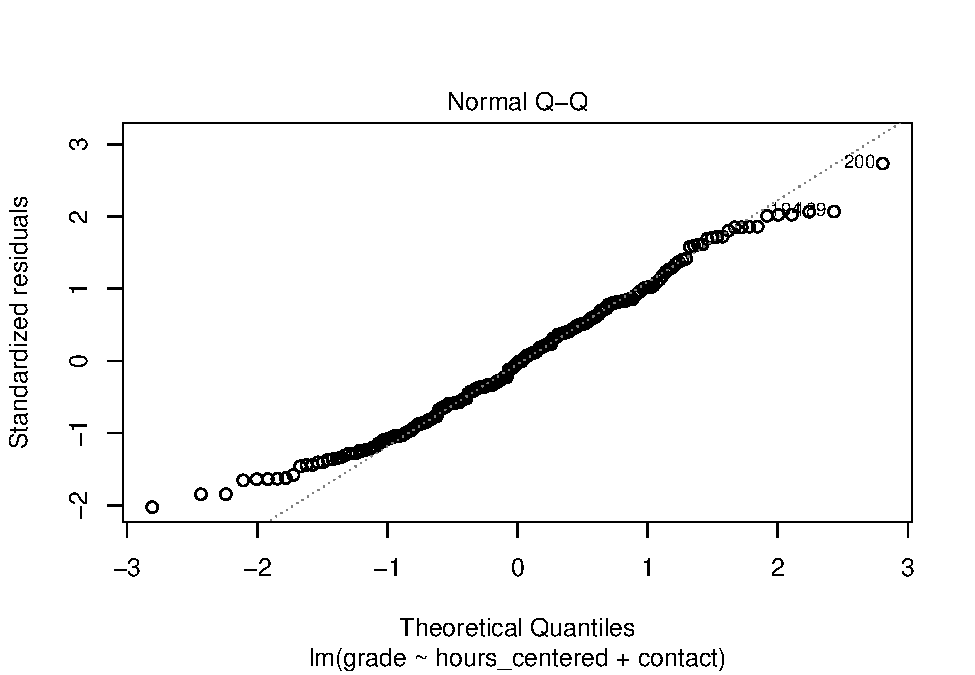
\includegraphics{_main_files/figure-latex/qq-1.pdf}

In the case of our model, most data points lie on the diagonal, while there are some small deviations in the tails. As our n is large enough, this should not be problematic. It may indicate that the model is not perfectly parsimonious but there is no clear cause for concern here.

\hypertarget{homoscedasticity}{%
\subsection{Homoscedasticity}\label{homoscedasticity}}

The \emph{homoscedasticity} assumption states that the residuals are expected to have a constant variance over the whole range of the dependent variable. Let us assume that the variance of our residuals would be lower for very good grades and higher for very bad ones. This would indicate that we can make more accurate estimates for better grades than for worse ones as a small variance would indicate smaller residuals and thus a smaller error. For the assumption to hold we must be able to make about the same quality of estimates, be it high or low, for all values of \texttt{grade}.

The problem is that the computation of the standard errors, test statistics and p-values depends on this assumption. If the assumption is violated, if we have \emph{heteroscedasticity}, these measures are not reliable anymore.

The problem often occurs when the dependent variable is not symmetric. In the scatterplot matrix above, we already saw that \texttt{grade} is fairly symmetrically distributed, so we would not expect problems here. If our dependent variable was asymmetrical, transforming it to be more symmetrical, e.g.~by using the logarithm or a square root, could help.

To check for problems with heteroscedasticity, we can use the \emph{Scale-Location} plot. This plots the fitted values against the square root of the standardized residuals. For homoscedasticity to hold, we should see our data points as a horizontal band with more or less constant width running from the left to the right. The same goes for the plotted line.

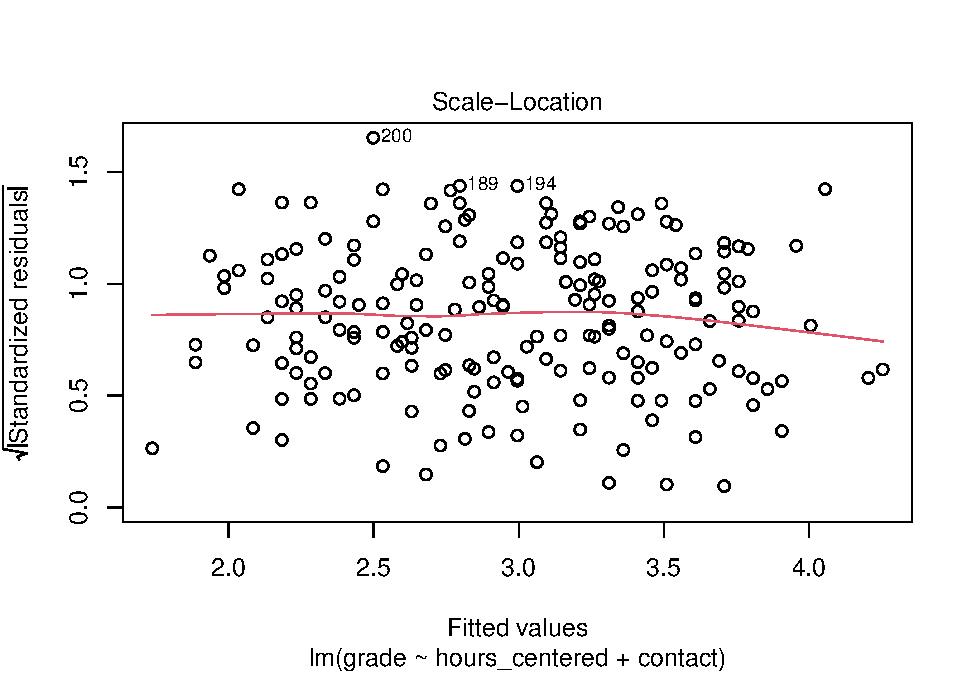
\includegraphics{_main_files/figure-latex/homoscedasticity-1.pdf}

In our case the homoscedasticity assumption holds. Slight variations are not problematic and overall the variance is constant.

\hypertarget{no-overly-influential-data-points}{%
\subsection{No overly influential data points}\label{no-overly-influential-data-points}}

Observations can get highly influential if they have unusual values. Sometimes these are extremely low or high values on some variable. But even ``normal'' values on two or more variables can get unusual in their combination. Imagine a student with \(60\) invested hours. A high value but not overly extreme. Now the same student had in person contact with their lecturer but still received a \(5.0\). This could potentially be an influential data point as this combination is unusual in terms of what the model expects. In case of our model this observation would most probably not be overly influential. But imagine the same observation with \(300\) invested hours. Such extreme cases can influence the fit by figuratively ``pulling'' the regression line in their direction.

We can divide influential data points into unusual values on the dependent variable, \emph{outliers}, and unusual values on independent variables, \emph{high leverage points}. The latter have high leverage because they ``pull'' on the regression lines and thus change the slope. As a rule of thumb, we can consider values with standardized residuals over \(3\) or under \(-3\) outliers. Concerning the dependent variables we can compute the \emph{leverage statistic}. Here values that exceed \(2 * (p + 1) / n\), where \(p\) is the number of predictors, are considered as having high leverage. We can inspect both at the same time in the \emph{Residuals vs.~Leverage} plot.

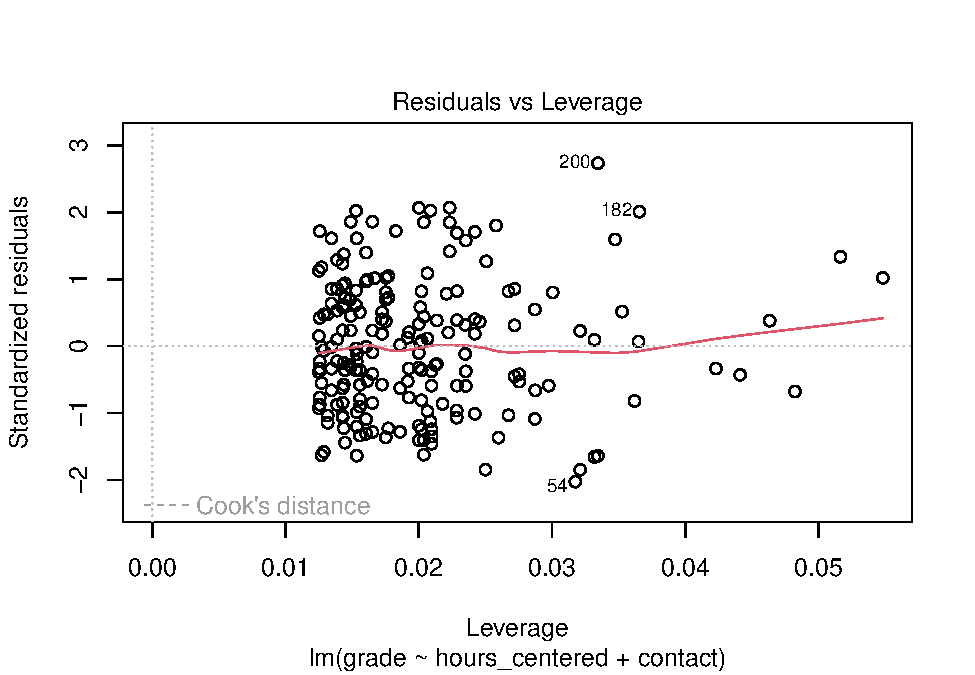
\includegraphics{_main_files/figure-latex/residuals_leverage-1.pdf}

We can see that there are no clear outliers. To assess points with high leverage we first have to compute the threshold as: \(2 * (3 + 1) / 200 = 0.04\). Note that while we have two independent variables in our model, we actually have three predictors due to our categorical variable. Thus we have to compute with \(p = 3\) instead of \(p = 2\). We can see that there are a number of points that exceed this value. The question is, why do these values exist? Sometimes these are measurement errors, extreme values or unusual combinations that come down to the researcher recording the wrong values into the data set. In these cases we can try to fix the errors or remove the observations from the data. As we have several values with high leverage, this seems highly unlikely. But if we had not simulated the data ourselves and knew that there is no error, we should at least check. What seems more probable though, and is often the actual root of high leverage, is that there are variables missing from the model that could explain the high values. In this case the values should be lower after we include the missing variables into the model. We will return to this later.

We also may not have a serious problem here. Leverage on its own does not have to be problematic. Some data points will always be more influential than others and remember that the cutoff is always just a rule of thumb. As said above, it is the combination of unusual values that tends to get problematic. We can check for observations that are outliers and have high leverage visually in our plot. Problematic observations tend to gather in the upper and lower right corners. As neither are populated for our model, we can not really conclude that we have overly influential data points.

\hypertarget{no-multicollinearity}{%
\subsection{No (multi)collinearity}\label{no-multicollinearity}}

The final assumption we will discuss here, is the absence of (high) collinearity between the predictor variables. \emph{Collinearity} is present, if two independent variables are highly correlated with each other. This can become a problem as it gets harder to individually estimate the effects for both variables on the outcome as the collinear variables vary together at the same time.

Often collinearity can already be spotted in the correlation matrix. Considering our matrix above we saw no clear indication that \texttt{hours} and \texttt{contact} are correlated. But the problem can get more complicated if we include three or more independent variables in our model. While none of the pairs of variables may be highly correlated, correlation may exist for a set of three or more of those variables. In these cases we speak of \emph{multicollinearity}. We can not spot this in a correlation matrix, but there is an easy to use measure available.

The \emph{variance inflation factor} (VIF) can be used to inspect (multi)collinearity between two or more independent variables accurately. A VIF of \(1\) would indicate no collinearity. For real world data this is almost never true as some amount of collinearity always exists. But in general we can say that the VIF should be near \(1\) and should not exceed a value of \(5\).

Let us compute the measure for our model with \texttt{hours\_centered} and \texttt{contact}:

\begin{verbatim}
## Warning: package 'car' was built under R version 4.2.3
\end{verbatim}

\begin{verbatim}
## hours_centered        contact 
##       1.004352       1.004352
\end{verbatim}

Both values are very close to \(1\) so we can conclude that we did not violate the assumption. But what could we do, if we did? One approach is to just delete one of the highly correlated independent variables from the model. As they vary together, it may be save to exclude one of them without losing to much information. Another approach would be to combine both variables into a new measure. Let us imagine that besides \texttt{contact} we would have another variable in our model, measuring how well a student feels supported by their lecturer in writing the paper. We could also imagine both variables being strongly correlated as they measure comparable concepts. We could then either drop one of the variables, maybe losing some information in the process, or we could combine both into a new variable which measures the form and the feeling of support at the same time, maybe leading to a more accurate estimate while at the same time eliminating the problem of collinearity. Which one is the right solution depends on the specific case.

\hypertarget{returning-to-our-research-question-1}{%
\section{Returning to our research question}\label{returning-to-our-research-question-1}}

When we tested for linearity above, we saw a mild pattern in the data which is not explainable by a violation of the assumption of linearity and thus could be an indication of a missing relevant explanatory variable in our model. Some of the other tests also supported this notion. The Q-Q plot showed us that the residuals have some slight deviations from normality in the tails. While these deviations are small enough to not cause concern on their own, taken together with the residuals vs.~fitted plot this gives more weight to the suspicion that some important variable is missing. We also identified some observations with high leverage. While we can rule out errors in our data, the high leverage could also be explainable by a missing variable.

But which variable could be missing from the model? If our DAG is correct, we can rule out \texttt{attendance} and \texttt{previous\_grades}. We did assume that \texttt{contact} is a confounder for \texttt{hours} and \texttt{grade} and thus included it in our model. Of course we could also miss a variable that is not in our data at all, or even one that is not measureable. As we did simulate the data, we know this is not true, but with real world data this is always a possibility.

Let us think about the \texttt{contact}variable once more. We did assume, that the more personal the contact, the more efficiently the time working on the paper can be used. And here may lie the problem. The way we included \texttt{contact} in the model is not the way we reasoned in our DAG. It would be correct if we assumed that the more personal the contact, the less time is invested. But we already saw in the scatterplot matrix that there is no such relationship between the variables. To specify the effect of \texttt{contact} in the model correctly, reflecting the idea of a more efficient use of time the closer the contact was, we have to include it as an interaction with \texttt{hours}.

\hypertarget{interactions}{%
\subsection{Interactions}\label{interactions}}

In an \emph{interaction}, we assume that the effect of one variable differs based on the value of another variable. Let us return to the formula for a multiple regression with two variables:

\[y = \beta_0 + \beta_1*x_1 + \beta_2*x_2 + \epsilon\]

Here we assume that the value of \(y\) varies with the value of \(x_1\) and \(x_2\) as indicated by the coefficients \(\beta_1\) and \(\beta_2\).

But we could also follow the notion that the value of \(x_1\) influences \(y\) differently based on the value of \(x_2\). For example the effect of \(x_1\) on \(y\) could be higher when \(x_2\) also has a high value. This is an interaction and is reflected in the formula by adding an additional multiplicative term between the two dependent variables with an additional associated coefficient:

\[y = \beta_0 + \beta_1*x_1 + \beta_2*x_2 + \beta_3 * x_1 * x_2 + \epsilon\]

To get a better understanding of this, let us return to our model and add an interaction between \texttt{hours\_centered} and \texttt{contact}.

\begin{verbatim}
## 
## Call:
## lm(formula = grade ~ hours_centered + contact + hours_centered * 
##     contact, data = grades)
## 
## Residuals:
##      Min       1Q   Median       3Q      Max 
## -1.77816 -0.72882 -0.08719  0.56140  2.53271 
## 
## Coefficients:
##                                 Estimate Std. Error t value Pr(>|t|)    
## (Intercept)                      3.44466    0.10345  33.298  < 2e-16 ***
## hours_centered                  -0.02893    0.01535  -1.885  0.06098 .  
## contactE-Mail                   -0.46775    0.16729  -2.796  0.00569 ** 
## contactIn Person                -1.01493    0.15171  -6.690 2.33e-10 ***
## hours_centered:contactE-Mail    -0.02377    0.02657  -0.895  0.37204    
## hours_centered:contactIn Person -0.05017    0.02442  -2.055  0.04125 *  
## ---
## Signif. codes:  0 '***' 0.001 '**' 0.01 '*' 0.05 '.' 0.1 ' ' 1
## 
## Residual standard error: 0.9253 on 194 degrees of freedom
## Multiple R-squared:   0.28,  Adjusted R-squared:  0.2615 
## F-statistic: 15.09 on 5 and 194 DF,  p-value: 1.63e-12
\end{verbatim}

How can we interpret these results? While the estimates for the intercept and for having e-mail or personal contact in comparison to having no contact at all have barely changed, the coefficient for the amount of hours invested substantially shrunk to almost half its former value. Until now we assumed that the effect of \texttt{hours} would be the same for each student. Now that we have included an interaction we assume that the effect of \texttt{hours} differs, based on the form of contact a student had.

Let us rewrite our formula for \(\hat{y}\) including the interaction. As we are interacting with a categorical variable with three categories, we have to add two interaction terms. The first for the effect of invested hours when e-mail contact was made and the second for the effect of hours when contact was made in person, in both cases compared to having had no contact.

\[\hat{y} = b_0 + b_{hours\_centered} * x_{hours\_centered} +\\
b_{E-Mail} * x_{E-Mail} + b_{In Person} * x_{In Person} +\\
b_{hours\_E-Mail} * x_{hours\_centered} * x_{E-Mail} +\\
b_{hours\_{In Person}} * x_{hours\_centered} * x_{In Person}\]

Let us now also add the coefficients from the model:

\[\hat{y} = 3.44466 -0.02893 * x_{hours\_centered} -\\
0.46775 * x_{E-Mail} -1.01493 * x_{In Person} -\\
0.02377 * x_{hours\_centered} * x_{E-Mail} -\\
0.05017 * x_{hours\_centered} * x_{In Person}\]

We can now consider the three possible forms of contact one by one.

What happens, when a student had no contact? To explore this, we return to the regression formula and equal \(x_{E-Mail}\) and \(x_{In Person}\) to \(0\), which means that no contact was made beforehand. Note that for now we do not care about the actual value of \texttt{hours\_centered}.

\[\hat{y} = 3.44466 -0.02893 *x_{hours\_centered} -\\
0.46775 * 0 -1.01493 * 0 -\\
0.02377 * x_{hours\_centered} * 0 -\\
0.05017 * x_{hours\_centered} * 0\]

This shortens to:

\[\hat{y} = 3.44466 -0.02893 *x_{hours\_centered}\]

For a student who did not make contact, we would estimate the final grade as the intercept minus \(0.02893\) per hour invested more than the mean of \texttt{hours\_centered}. Having equaled \(x_{E-Mail}\) and \(x_{In Person}\) to \(0\) not only ``switched off'' the effects of \texttt{contact} but also removed the interaction effects from the equation, the estimated effect for \texttt{hours\_centered} is only its coefficient of \(-0.02893\).

What happens, when a student had e-mail contact?

\[\hat{y} = 3.44466 -0.02893 * x_{hours\_centered} -\\
0.46775 * 1 -1.01493 * 0 -\\
0.02377 * x_{hours\_centered} * 1 -\\
0.05017 * x_{hours\_centered} * 0\]

This shortens to:

\[\hat{y} = 3.44466 -0.02893 *x_{hours\_centered} -\\
0.46775 -\\
0.02377 * x_{hours\_centered}\]

and further to:

\[\hat{y} = 2.97691 -0.0527 *x_{hours\_centered}\]

The intercept is reduced by the coefficient of having e-mail contact, but what is actually of interest here is the effect that \texttt{hours\_centerd} has. For a student who had e-mail contact, each hour invested above the mean reduces the estimated grade by \(-0.0527\).

We can compute the same for a student with personal contact:

\[\hat{y} = 3.44466 -0.02893 * x_{hours\_centered} -\\
0.46775 * 0 - 1.01493 * 1  -\\
0.02377 * x_{hours\_centered} * 0 -\\
0.05017 * x_{hours\_centered} * 1\]

\[\hat{y} = 3.44466 -0.02893 *x_{hours\_centered} -\\
1.01493 -\\
0.05017 * x_{hours\_centered}\]

\[\hat{y} = 2.42973 -0.0791 *x_{hours\_centered}\]

For a student who had in person contact, each hour invested above the mean reduces the estimated grade by \(-0.0791\).

In practice we would have reached these conclusions more quickly by inspecting the output from our model and just subtracting the corresponding interaction effect from the effect for \texttt{hours\_centered}, but it is important to understand what happens in the formula to get a full grasp on linear regression models.

In the model without the added interaction we concluded that on average each hour invested above the mean decreases the final grade by about \(-0.5\). Now we see that the effect of hours depends on the form of contact had. This reflects the theoretical assumption from our DAG that time can be used more efficiently the more personal the form of contact was.

The same DAG that informed our best model from last week now lead us to including the interaction. This underlines the importance of thorough theoretical thinking before starting to model. It was not even the case that the DAG was wrong, but our conclusions we drew from it were at least not completely right. If we had invested more time, we could have build the correct model directly. In our case we first needed the regression diagnostics to tell us that something might be off before we figured out our error.

\hypertarget{regression-diagnostics-revisited}{%
\subsection{Regression diagnostics (revisited)}\label{regression-diagnostics-revisited}}

We now have a theoretically sound model, but did we also solve the problems indicated in the regression diagnostics?

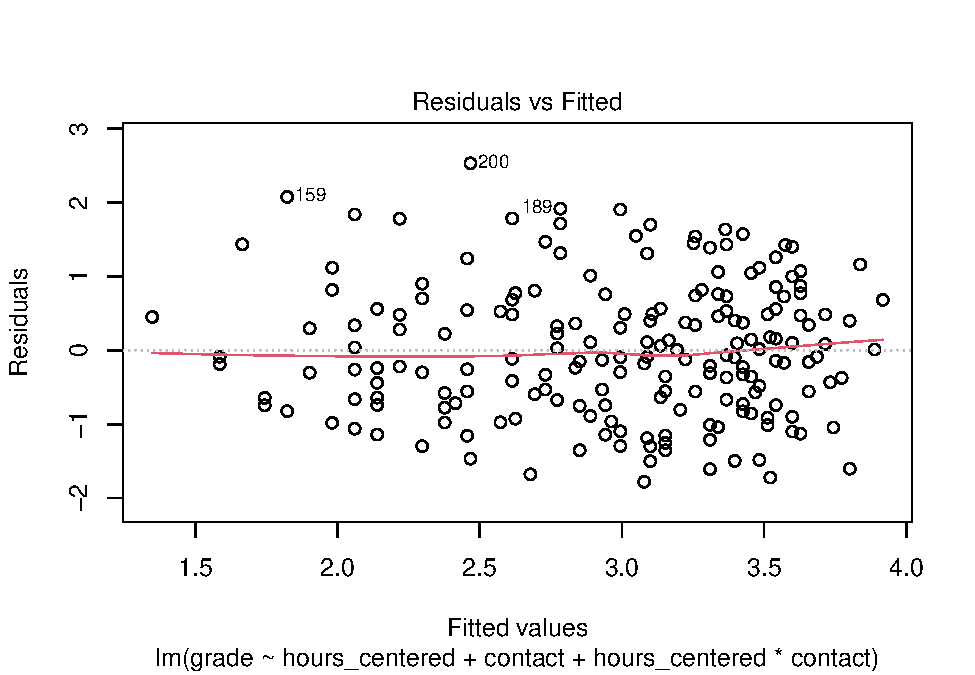
\includegraphics{_main_files/figure-latex/residuals_fitted_revisit-1.pdf}

The residuals vs.~fitted plot now shows an almost straight horizontal line with no clear visible patterns. This indicates that the problem we saw with our former model actually came down to a missing variable, or to be more precise a missing term in our case.

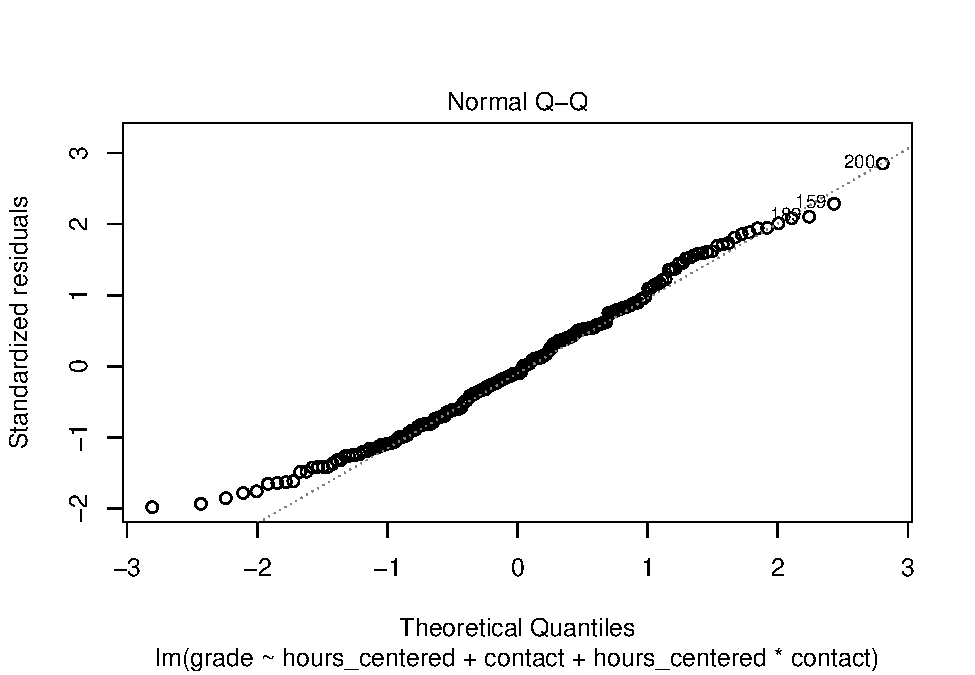
\includegraphics{_main_files/figure-latex/qq_revisited-1.pdf}

The Q-Q plot now also shows more normally distributed residuals. While there are still some small deviations at the lower tail these do not indicate a remaining severe problem. The deviations are smaller than before and also not drastic in absolute terms. Also, as stated above, violating the normality assumption is less problematic with a high \(n\) and few variables in the model, which is still true for our case.

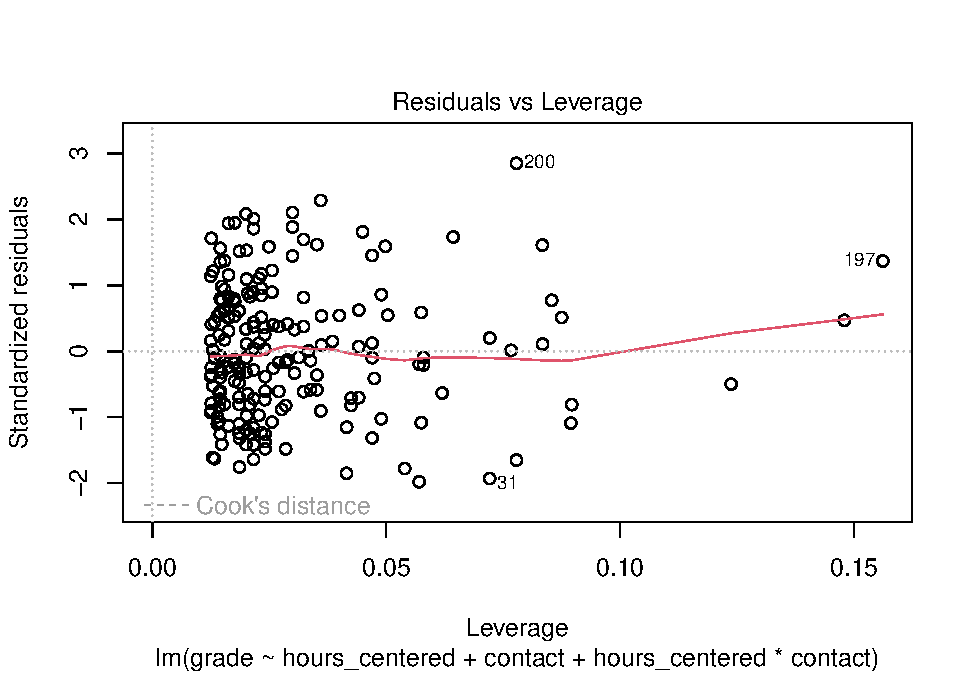
\includegraphics{_main_files/figure-latex/residuals_leverage_revisited-1.pdf}

Adding the interaction term actually increased the leverage of the more influential observations. When we recompute the threshold as \(2 * (5 + 1) / 200 = 0.06\), we see that there still some observations with values higher than this. What has not changed, is that there are no clusters of observations in the lower or upper right corners. Overall we can conclude, that this problem is present but negligible. When there are observations that are problematic on both values at the same time, these also get marked by a red dashed line in the plot. This is also not present.

\hypertarget{conclusion}{%
\section{Conclusion}\label{conclusion}}

Over the last three sessions we have learned what a linear regression is, how its formula works, how to interpret the results for different kinds of variables as well as how to check and correct violations of its underlying assumptions.

At the same time we built a model, which in its final version is able to accurately estimate our effect of interest. But we had one immeasurable advantage: We simulated the data ourselves and thus knew where the journey was going to end up from the start. We knew our DAG was correct because the data was simulated in this way and we also knew that there was going to be a interaction effect to solve the remaining diagnostic problems. Sneaky, right? But in real world data, we do not have these advantages. Our DAGs can be incorrect and we may or may not find the missing part of the puzzle that elevates an OK model to a great one. All we can do is think, explore our data, think again, run diagnostics, think again and maybe most importantly do not give up along the way.

In the \protect\hyperlink{lin-a}{next session} we will return to our NBA data and try to apply everything that we have learned over the last sessions.

\hypertarget{resources-1}{%
\section{Resources}\label{resources-1}}

Most textbooks on statistics include introductions and discussion on using linear regressions. The following resources were the ones actually used in writing the last three sessions:

The textbook from Kohler and Kreuter gives a thorough introduction to linear regression and other statistical concepts. While all code examples are written in Stata, the underlying statistics are the same, no matter the coding language. The book is also available in English.

Kohler, Ulrich \& Frauke Kreuter (2017). Datenanalyse mit Stata. Allgemeine Konzepte der Datenanalyse und ihre praktische Anwendung. 5. aktualisierte Auflage. Berlin, Boston: De Gruyter Oldenbourg.

\hfill\break

James, Gareth; Daniela Witten; Trevor Hastie \& Robert Tibshirani (2021). An Introduction to Statistical Learning. with Applications in R. Second Edition. New York: Springer.

\hfill\break

Manderscheid, Katharina (2017). Sozialwissenschaftliche Datenanalyse mit R. Eine Einführung. 2. Auflage.Wiesbaden: Springer VS.

\hypertarget{lin-a}{%
\chapter{Linear Regression - Application}\label{lin-a}}

\textbf{Still WIP!}

After we have learned the ins and outs of linear regression we will now
return to our NBA data.
We already saw, that there was an interesting relationship between the
points a player makes per game and the salary he receives in \protect\hyperlink{eda-1}{session 2}. In
\protect\hyperlink{dags-1}{session 4} we also built a DAG that reflects our assumptions about the data
generating process. Based on the DAGs implications we can now build a linear
regression model and try to estimate the effect of interest as accurately as
possible.

\hypertarget{objectives-5}{%
\section{Objectives}\label{objectives-5}}

\begin{itemize}
\tightlist
\item
  Estimate the effect of interest, scored point on salary, using a linear regression
\item
  Applying diagnostics to the model and correct mistakes
\item
  Interpret the final model
\end{itemize}

\hypertarget{r-functions-covered-this-week-1}{%
\section{R functions covered this week}\label{r-functions-covered-this-week-1}}

\begin{itemize}
\tightlist
\item
  \texttt{lm()} : This function is used to fit a linear model to the data. It takes a formula that specifies the dependent and independent variables, and a data frame that contains the variables. It returns a model object that can be used for further analysis.
\item
  \texttt{summary()} : This function is used to get a summary of a model object, such as the coefficients, standard errors, t-values, p-values, R-squared, and F-statistic. It also provides information on the residuals, such as the minimum, maximum, median, and quartiles.
\item
  \texttt{tidy()} : This function is from the \textbf{broom} package. It is used to convert a model object into a tidy tibble that contains one row per parameter estimate and columns for the term, estimate, standard error, statistic, and p-value.
\item
  \texttt{plot()} : This function is used to create various plots for a model object, such as the residuals vs fitted values, the Q-Q plot, the scale-location plot, and the residuals vs leverage plot. These plots are useful for checking the assumptions of linear regression, such as linearity, normality, homoscedasticity, and outliers¹{[}1{]}.
\item
  \texttt{autoplot()} : This function is from the \textbf{ggfortify} package. It is used to create the same plots as \texttt{plot()} but in the style of \textbf{ggplot2}. It returns a list of four plots that can be customized further with \textbf{ggplot2} functions.
\item
  \texttt{vif()} : This function is from the \textbf{car} package. It is used to compute the variance inflation factors (VIF) for each independent variable in a linear model. The VIF measures how much the variance of a coefficient estimate is inflated due to multicollinearity. A high VIF indicates a potential problem of multicollinearity.
\item
  \texttt{log()} : This function is used to compute the natural logarithm of a numeric vector. It can be used to transform a skewed dependent variable into a more normal distribution²{[}2{]}.
\item
  \texttt{I()} : This function is used to indicate that an expression should be evaluated as it is in a formula. It can be used to include non-linear transformations or interactions of independent variables in a linear model³{[}3{]}.
\item
  \texttt{exp()} : This function is used to compute the exponential function of a numeric vector. It can be used to reverse the logarithmic transformation of a dependent variable.
\item
  \texttt{ggplot()}: It's a key function from the \emph{ggplot2} package and is used to create a wide variety of static, dynamic, and interactive graphics in R. The function allows you to specify a mapping from data to aesthetics (color, shape, size) and geometric objects (points, lines, bars). It also allows you to add statistical transformations, coordinate systems, faceting, and themes.
\item
  \texttt{glance()} : This function is from the \textbf{broom} package. It is used to get a summary of a model object, such as the R-squared, adjusted R-squared, RMSE, p-value, etc. It takes a model object and returns a tibble with one row per model and one column per statistic.
\end{itemize}

\hypertarget{research-question}{%
\section{Research question}\label{research-question}}

Picking up from session 2 \& 4, our research question is still to get an unbiased
estimate for the effect from points scored on the salary a NBA player receives.
We already constructed a DAG that reflects our assumptions for the underlying
data generating process. Let us revisit this briefly:

\includegraphics{_main_files/figure-latex/dag_final-1.pdf}

The implications of our DAG were that we only have to control for the position
a player occupies to get an unbiased estimate for our effect of interest.
The path that passes the body height is already closed by controlling for
position and the team a player plays for as well as the season an observation
was recorded in do not lie on an paths from our main independent to our
dependent variable.
Based on this we construct our model.

Now let us get to it and load the NBA data we prepared in week 2.

\begin{Shaded}
\begin{Highlighting}[]
\FunctionTok{library}\NormalTok{(tidyverse)}
\FunctionTok{load}\NormalTok{(}\StringTok{"../datasets/nba/data\_nba.RData"}\NormalTok{)}
\end{Highlighting}
\end{Shaded}

\hypertarget{simple-linear-regression-in-r}{%
\section{Simple linear regression in R}\label{simple-linear-regression-in-r}}

To conduct a multiple linear regression in R, we can use the built-in \emph{base R}
function \texttt{lm()}, short for \emph{linear model}.
The function is straightforward to use. As the first argument
we write the regression formula in R's \emph{formula syntax}.

We start building the formula by writing the name of our \texttt{dependent\_variable}
followed by a \emph{tilde} \texttt{\textasciitilde{}}. You can read this as an \(=\) or as ``regress the
dependent variable on''. After the tilde we add our first \texttt{indepedent\ variable}
by again writing out its name. If we have multiple independent variables in our
model - when we are running a \emph{multiple linear regression} - we can add those by
writing a \texttt{+} followed by the name of the variable to be added.

As an additional argument, the function needs the name of the object that holds our
data.

The goal of our research question is to estimate the effect of the points per
game on the received salary. So to regress \texttt{salary} on \texttt{career\_PTS}, we just
write:

\begin{Shaded}
\begin{Highlighting}[]
\FunctionTok{lm}\NormalTok{(salary }\SpecialCharTok{\textasciitilde{}}\NormalTok{ career\_PTS, }\AttributeTok{data =}\NormalTok{ data\_nba)}
\end{Highlighting}
\end{Shaded}

\begin{verbatim}
## 
## Call:
## lm(formula = salary ~ career_PTS, data = data_nba)
## 
## Coefficients:
## (Intercept)   career_PTS  
##     -851914       552843
\end{verbatim}

This gives us a short output. The first line just echoes our code used to run
the regression. We have seen this in the last session already, but now we know
what the meaning was. After this we have a short block with the estimated
coefficients. As we have run a simple linear regression, we only get the
intercept and the coefficient for the sole independent variable used in the
model. If we would have run a multiple linear regression, the result would
basically look the same, only with more coefficients to display.

Before we dive into the results, we should talk about how to receive a more
verbose output that does not hide all the other vital information that is
associated with the model.

The easiest way is to use the base R function \texttt{summary()}. This is a generic R
function that returns different summaries, depending on the object it is used
on. We can for example use it on a data frame or tibble to get some descriptive
statistics for the included variables. For example, we can get information on the
distribution of points per game by writing:

\begin{Shaded}
\begin{Highlighting}[]
\FunctionTok{summary}\NormalTok{(data\_nba}\SpecialCharTok{$}\NormalTok{career\_PTS)}
\end{Highlighting}
\end{Shaded}

\begin{verbatim}
##    Min. 1st Qu.  Median    Mean 3rd Qu.    Max. 
##   0.000   5.100   8.000   8.908  12.000  30.100
\end{verbatim}

When we use \texttt{summary()} on a model object, like the one created by \texttt{lm()}, we
get a different output. Before we apply this we should save our model in an
object. This is good practice in most cases, as we can now apply all additional
analysis of the model on this object and we do not have to rerun the model
every time.

\begin{Shaded}
\begin{Highlighting}[]
\NormalTok{m1 }\OtherTok{\textless{}{-}} \FunctionTok{lm}\NormalTok{(salary }\SpecialCharTok{\textasciitilde{}}\NormalTok{ career\_PTS, }\AttributeTok{data =}\NormalTok{ data\_nba)}
\end{Highlighting}
\end{Shaded}

We can now apply \texttt{summary()} on the object \texttt{m1}, short for ``model 1'':

\begin{Shaded}
\begin{Highlighting}[]
\FunctionTok{summary}\NormalTok{(m1)}
\end{Highlighting}
\end{Shaded}

\begin{verbatim}
## 
## Call:
## lm(formula = salary ~ career_PTS, data = data_nba)
## 
## Residuals:
##       Min        1Q    Median        3Q       Max 
## -14788659  -2023969   -434599   1311807  24326060 
## 
## Coefficients:
##             Estimate Std. Error t value Pr(>|t|)    
## (Intercept)  -851915      76417  -11.15   <2e-16 ***
## career_PTS    552843       7453   74.17   <2e-16 ***
## ---
## Signif. codes:  0 '***' 0.001 '**' 0.01 '*' 0.05 '.' 0.1 ' ' 1
## 
## Residual standard error: 3732000 on 9726 degrees of freedom
## Multiple R-squared:  0.3613, Adjusted R-squared:  0.3612 
## F-statistic:  5502 on 1 and 9726 DF,  p-value: < 2.2e-16
\end{verbatim}

This is the output we saw over the last weeks and it includes an extended and
better readable coefficient block as well as the information on the residuals
and the model fit.

An alternative method of displaying the coefficients in a regular tibble format
is to use \texttt{tidy()} from the \texttt{broom} package.

\begin{Shaded}
\begin{Highlighting}[]
\FunctionTok{library}\NormalTok{(broom)}

\FunctionTok{tidy}\NormalTok{(m1)}
\end{Highlighting}
\end{Shaded}

\begin{verbatim}
## # A tibble: 2 x 5
##   term        estimate std.error statistic  p.value
##   <chr>          <dbl>     <dbl>     <dbl>    <dbl>
## 1 (Intercept) -851914.    76417.     -11.1 1.09e-28
## 2 career_PTS   552843.     7453.      74.2 0
\end{verbatim}

\hypertarget{interpretation}{%
\subsection{Interpretation}\label{interpretation}}

While we know our model is not complete yet, let us still inspect the results.
For each point a player scores per game, his salary rises by about \(552,000\$\).
We see a clear positive and substantial effect. Let us also inspect the
intercept. This tells us that a player who makes no points per game has to pay
the team about \(850,000\). Wait, this does not make sense\ldots{}
To make the intercept more readily interpretable we should again center our
metric dependent variable \texttt{career\_PTS} on its mean.

\begin{Shaded}
\begin{Highlighting}[]
\FunctionTok{mean}\NormalTok{(data\_nba}\SpecialCharTok{$}\NormalTok{career\_PTS)}
\end{Highlighting}
\end{Shaded}

\begin{verbatim}
## [1] 8.907679
\end{verbatim}

\begin{Shaded}
\begin{Highlighting}[]
\NormalTok{data\_nba }\OtherTok{\textless{}{-}}\NormalTok{ data\_nba }\SpecialCharTok{\%\textgreater{}\%} 
  \FunctionTok{mutate}\NormalTok{(}\AttributeTok{PTS\_centered =}\NormalTok{ career\_PTS }\SpecialCharTok{{-}} \FunctionTok{mean}\NormalTok{(career\_PTS))}
\end{Highlighting}
\end{Shaded}

As we have now centered the independent variable of interest on its mean of \(8.9\)
we can rerun the model.

\begin{Shaded}
\begin{Highlighting}[]
\NormalTok{m1 }\OtherTok{\textless{}{-}} \FunctionTok{lm}\NormalTok{(salary }\SpecialCharTok{\textasciitilde{}}\NormalTok{ PTS\_centered, }\AttributeTok{data =}\NormalTok{ data\_nba)}

\FunctionTok{summary}\NormalTok{(m1)}
\end{Highlighting}
\end{Shaded}

\begin{verbatim}
## 
## Call:
## lm(formula = salary ~ PTS_centered, data = data_nba)
## 
## Residuals:
##       Min        1Q    Median        3Q       Max 
## -14788659  -2023969   -434599   1311807  24326060 
## 
## Coefficients:
##              Estimate Std. Error t value Pr(>|t|)    
## (Intercept)   4072633      37840  107.63   <2e-16 ***
## PTS_centered   552843       7453   74.17   <2e-16 ***
## ---
## Signif. codes:  0 '***' 0.001 '**' 0.01 '*' 0.05 '.' 0.1 ' ' 1
## 
## Residual standard error: 3732000 on 9726 degrees of freedom
## Multiple R-squared:  0.3613, Adjusted R-squared:  0.3612 
## F-statistic:  5502 on 1 and 9726 DF,  p-value: < 2.2e-16
\end{verbatim}

The coefficient for points per game has not changed but its interpretation has.
For each point per game over the mean of \(8.9\) points per game, the salary is
estimated to increase by about \(552,000\$\). At the same time, for each point
below the mean the salary is estimated to decrease by the same amount.
The intercept now shows us the estimated salary of a player who scores \(8.9\)
points per game, which is slightly upwards of \(4,000,000\$\). This makes way more
sense.

This model model already achieved a considerable \(R^2\) of \(0.36\). About \(36\%\)
of the variance in salaries is explained by points per game.

Another way to get the model statistics, such as \(r^2\), F-statistic, and p-value, is to use the \texttt{glance()} function from the broom package. This function returns a tibble with one row of model summaries.

\begin{Shaded}
\begin{Highlighting}[]
\FunctionTok{glance}\NormalTok{(m1)}
\end{Highlighting}
\end{Shaded}

\begin{verbatim}
## # A tibble: 1 x 12
##   r.squared adj.r.squared    sigma statistic p.value    df  logLik    AIC    BIC
##       <dbl>         <dbl>    <dbl>     <dbl>   <dbl> <dbl>   <dbl>  <dbl>  <dbl>
## 1     0.361         0.361 3732168.     5502.       0     1 -1.61e5 3.22e5 3.22e5
## # i 3 more variables: deviance <dbl>, df.residual <int>, nobs <int>
\end{verbatim}

We can see that the output includes the same information as the summary of \texttt{m1}, but in a different format. The advantage of using \texttt{glance()} is that it is easier to manipulate and compare the model statistics using tidyverse functions. For example, we can use \texttt{bind\_rows()} to combine the outputs of different models and compare their performance.

\hypertarget{multiple-linear-regression-in-r}{%
\section{Multiple linear regression in R}\label{multiple-linear-regression-in-r}}

The DAG we have constructed above based on our research question indicated that
we also have to include the position a player occupies in our model.
We can add additional independent variables to the formula used in \texttt{lm()} with a
\texttt{+} and the name of the additional variable(s). This works the same way for all
types of variables, i.e.~metric, dummies or categorical variables.
So let us do this now by adding the 5 dummies we constructed for the positions:

\begin{Shaded}
\begin{Highlighting}[]
\NormalTok{m2 }\OtherTok{\textless{}{-}} \FunctionTok{lm}\NormalTok{(salary }\SpecialCharTok{\textasciitilde{}}\NormalTok{ PTS\_centered }\SpecialCharTok{+}\NormalTok{ position\_center }\SpecialCharTok{+}\NormalTok{ position\_sf }\SpecialCharTok{+}\NormalTok{  position\_pf }\SpecialCharTok{+}\NormalTok{ position\_sg }\SpecialCharTok{+}\NormalTok{ position\_pg, }\AttributeTok{data =}\NormalTok{ data\_nba)}

\FunctionTok{summary}\NormalTok{(m2)}
\end{Highlighting}
\end{Shaded}

\begin{verbatim}
## 
## Call:
## lm(formula = salary ~ PTS_centered + position_center + position_sf + 
##     position_pf + position_sg + position_pg, data = data_nba)
## 
## Residuals:
##       Min        1Q    Median        3Q       Max 
## -14511723  -1950255   -372906   1358768  24433660 
## 
## Coefficients:
##                 Estimate Std. Error t value Pr(>|t|)    
## (Intercept)      3679728     114300  32.193  < 2e-16 ***
## PTS_centered      568019       7474  75.994  < 2e-16 ***
## position_center  1380246     114539  12.050  < 2e-16 ***
## position_sf       125384     102174   1.227 0.219790    
## position_pf       206505      94882   2.176 0.029547 *  
## position_sg      -331033      96841  -3.418 0.000633 ***
## position_pg      -114552     117486  -0.975 0.329572    
## ---
## Signif. codes:  0 '***' 0.001 '**' 0.01 '*' 0.05 '.' 0.1 ' ' 1
## 
## Residual standard error: 3652000 on 9721 degrees of freedom
## Multiple R-squared:  0.3888, Adjusted R-squared:  0.3884 
## F-statistic:  1031 on 6 and 9721 DF,  p-value: < 2.2e-16
\end{verbatim}

\hypertarget{interpretation-1}{%
\subsection{Interpretation}\label{interpretation-1}}

We still see a clear positive effect of points per game on the received salary
after controlling for the position a player occupies. Among those centers are by
far the top earners, making about \(1,400,00\$\) more than players on other
positions. Most other positions show relatively small effects on the earnings.
Power and small forwards earn somewhat more than other positions on average
while point and especially shooting guards earn less.

We can now compare two fictive cases of a center and a point guard who each make
about \(20\) points per game. What is the estimated salary for them?

As we have extensively worked with the formulas over the last sessions, we can
now keep it short and calculate the estimate directly. Remember that we
centered the points per game on the mean of about \(8.9\), so making \(20\) per game
would mean scoring about \(11.1\) more compared to the average player. We will keep it simple
here and calculate with \(11\).

\[\hat{y_{center\_20}} = 3679728 + 568019 * 11 + 1380246 = 11,308,183\]

\[\hat{y_{pg\_20}} = 3679728 + 568019 * 11 - 114552 = 9,813,385\]

Despite making the same amount of points per game for their team, the model
estimates that a point guard earns about \(1,500,000\$\) less compared to a center.

\hypertarget{sidenote-adding-interactions}{%
\subsection{Sidenote: Adding interactions}\label{sidenote-adding-interactions}}

We will not use interactions in this session but we briefly want to state how we
could add them in the formula syntax.

Remember that interactions are multiplicative terms in our regression formula.
Adding them to the R formula syntax works the same way. We add the new term with
a \texttt{+} and use a \texttt{*} between the two variables that we want to interact.

Here is a non running toy example where we interact two x-variables:

\begin{verbatim}
lm(y ~ x1 + x2 + x1 * x2, data = some_data)
\end{verbatim}

\hypertarget{regression-diagnostics-1}{%
\section{Regression Diagnostics}\label{regression-diagnostics-1}}

So how does our model perform? Did we meet all the regression assumptions that
were introduced last week?

To access the visual tests we used last session, we can just use the base R
function \texttt{plot()}, applied to the model object. If we write \texttt{plot(m2)}, the
console asks us to press \texttt{ENTER} to go through each plot one by one. We can also
add a number as a second argument, specifying which plot we want to see. For
example, \texttt{plot(m2,\ 1)} gives us the residuals vs.~fitted plot.

But there is an easier way to see all four plots at once. The package
\texttt{ggfortify} expands the functionalities of \texttt{ggplot2} so that we can use it's
\texttt{autoplot()} function to automatically plot all four visual tests of interest.
An added benefit, depending on your taste, is that the plots are rendered in the
style of \texttt{ggplot2}.

\begin{Shaded}
\begin{Highlighting}[]
\FunctionTok{library}\NormalTok{(ggfortify)}

\FunctionTok{autoplot}\NormalTok{(m2)}
\end{Highlighting}
\end{Shaded}

\includegraphics{_main_files/figure-latex/m2_diag-1.pdf}

The residuals vs.~fitted does not show us a more or less straight line but
starts mildly positive, then dips below \(0\) and rises again for higher estimated
salaries. This could indicate at least two thing. Either we have missed an
important independent variable, like in the last session, or we are actually
dealing with some amount on non-linearity. If it is non-linearity, it is still
\emph{mild} non-linearity, but maybe we should still inspect this.

The Q-Q plot this time shows that the actual residuals are far from being
distributed normally. While we can never expect a perfectly normal distribution,
here the deviations are striking, especially for high residuals.

The scale-location plot is used to address the assumption of homoscedasticity.
What we want to see, is a straight line with data points equally distributed
around it. This clearly is not the case here. As it is, the plot indicates
that we may be able to estimate small salaries reasonably well but that the
higher the estimate, the more unreliable our model gets.

The residuals vs.~leverage plot also indicates some problems. There are some
observations that have larger or smaller standardized residuals compared to the
thresholds of \(3\) and \(-3\). The threshold for leverage is computed as
\(2 * (6 + 1) / 9728 = 0.001439145\). We also see some observations with higher
values. While both are rules of thumb and may not necessarily point to severe
problems by themselves, things can get problematic when there are observations
that do not meet the thresholds for both measures at the same time. This is
indicated by clusters in the lower or upper right corners. This time we can
observe this in the lower right.

We should also test for multicollinearity. We can compute the VIF measures using
a function from the package \texttt{car}.

\begin{Shaded}
\begin{Highlighting}[]
\FunctionTok{library}\NormalTok{(car)}

\FunctionTok{vif}\NormalTok{(m2)}
\end{Highlighting}
\end{Shaded}

\begin{verbatim}
##    PTS_centered position_center     position_sf     position_pf     position_sg 
##        1.050400        2.035722        1.686736        1.512765        1.565004 
##     position_pg 
##        1.916933
\end{verbatim}

The values for any variable should not exceed \(5\) and should be closer to \(1\).
Our value for points shows no signs of multicollinearity. The values for the
position dummies have somewhat higher values, which makes sense. While there are
some players that play multiple positions, for most a value of \(1\) on one
position predicts the other positions as having a value of \(0\). But as we are
still far away from the threshold of \(5\), there is no need for concern here.

Overall, we have problems! While we do not see signs of problematic
multicollinearity, all other tests indicated clear and in parts severe problems.
We have to put in some more work before we can be confident that our model
accurately estimates the effect of points per game on the received salary.

Before we start addressing the problems, we should note that the four plots are
highly interactive. It is entirely possible that solving one of the problems
also solves the others or, for added fun, even generates new ones. This means
that we should refrain from turning too many dials at once and rather change the
model one step at a time, see if it improves things and then address remaining
problems in the same way.

\hypertarget{skewed-outcome-variable}{%
\subsection{Skewed outcome variable}\label{skewed-outcome-variable}}

The deviation from normality and the clearly present heteroscedasticity could
both point to the same problem, namely a skewed dependent variable. Let us
examine its distribution first.

\begin{Shaded}
\begin{Highlighting}[]
\NormalTok{data\_nba }\SpecialCharTok{\%\textgreater{}\%} 
  \FunctionTok{ggplot}\NormalTok{(}\FunctionTok{aes}\NormalTok{(}\AttributeTok{x =}\NormalTok{ salary)) }\SpecialCharTok{+}
  \FunctionTok{geom\_density}\NormalTok{()}
\end{Highlighting}
\end{Shaded}

\includegraphics{_main_files/figure-latex/distribution_dv_before-1.pdf}

Our outcome variable is not only skewed, it is \textbf{highly skewed}. While there
are many salaries in the ``lower'' six to seven digits regions, we also see some
extremely high wages up to about \(35,000,000\$\). The higher the salary the fewer
observations we have. That is why we see such a long flat tail to the right.

This distribution actually is relatively common for income data. In most surveys
of the general population we have many people receiving relatively low incomes
while fewer individuals receive higher or extremely high incomes. It is still
interesting that this also holds true for a population of high earners such as
NBA players. Inequality is relative. Compared to the general
population almost all our players would be somewhere in the long tail to the
right. Compared to their own population we still see highly substantial
differences in outcomes.

We can transform the dependent variable to a different scale to get a less
skewed distribution. A common transformation for income data is to take the
\emph{logarithmus naturalis} of the actual value and then use this as our
dependent variable. To achieve the transformation we can simply use the base R
function \texttt{log()} which as its default computes the \(ln\).

\begin{Shaded}
\begin{Highlighting}[]
\NormalTok{data\_nba }\OtherTok{\textless{}{-}}\NormalTok{ data\_nba }\SpecialCharTok{\%\textgreater{}\%} 
  \FunctionTok{mutate}\NormalTok{(}\AttributeTok{salary\_log =} \FunctionTok{log}\NormalTok{(salary))}

\NormalTok{data\_nba }\SpecialCharTok{\%\textgreater{}\%} 
  \FunctionTok{ggplot}\NormalTok{(}\FunctionTok{aes}\NormalTok{(}\AttributeTok{x =}\NormalTok{ salary\_log)) }\SpecialCharTok{+}
  \FunctionTok{geom\_density}\NormalTok{()}
\end{Highlighting}
\end{Shaded}

\includegraphics{_main_files/figure-latex/transform_dv_log-1.pdf}

While the distribution of the transformed variable also is somewhat skewed, now
to the left, overall it is much more evenly distributed.

We should use the new variable as our outcome an check the tests again.

\begin{Shaded}
\begin{Highlighting}[]
\NormalTok{m3 }\OtherTok{\textless{}{-}} \FunctionTok{lm}\NormalTok{(salary\_log }\SpecialCharTok{\textasciitilde{}}\NormalTok{ PTS\_centered }\SpecialCharTok{+}\NormalTok{ position\_center }\SpecialCharTok{+}\NormalTok{ position\_sf }\SpecialCharTok{+}\NormalTok{  position\_pf }\SpecialCharTok{+}\NormalTok{ position\_sg }\SpecialCharTok{+}\NormalTok{ position\_pg, }\AttributeTok{data =}\NormalTok{ data\_nba)}

\FunctionTok{autoplot}\NormalTok{(m3)}
\end{Highlighting}
\end{Shaded}

\includegraphics{_main_files/figure-latex/m3-1.pdf}

Looking at the scale-location plot first, we can now see a straight line with
our residuals fairly evenly distributed around it. Thus we now longer see any
signs of heteroscedasticity. The Q-Q plot now also indicates a somewhat more
normal distribution of our residuals but there are substantial deviations still.
While high residuals now appear to more or less follow the normal distribution,
small residuals now deviate stronger than they have before. This reflects the
transformation and its distribution, which now has long tail on the left instead of
on the right, as before. Turning to the residuals vs.~leverage plot we still see
some observations that do not meet the respective thresholds. At the same time,
there appear to be less that simultaneously have high absolute standardized
residuals and high leverage. The residuals vs.~fitted plot now also shows a more
even distribution while the signs on non-linearity remain. We do not have to
recompute the VIF measure as we did not change any independent variables in the
model.

\hypertarget{non-linearity}{%
\subsection{Non-linearity}\label{non-linearity}}

Let us now address the non-linearity that is still indicated in the first plot.
We can approach non-linear relationships in our inherently linear model by
adding non-linear transformations of a dependent variable to the model. But
before we start squaring random variables, we should think about what could be
non-linear in our case. We can rule out our dummy variables for position. This
leaves the points scored. The model already indicates that our suspicion that
salary rises with the points scored could be true. But maybe this relationship
is not linear over its whole range. If you already are among high scorers,
scoring one or two points more than your peers may not be such a substantial
difference and thus may not have the same strong effect on salary.

We should first inspect the relationship between both variables again. This time
we add a LOWESS curve to the plot. This is often helpful in detecting
non-linearity as the curve can change its slope over the range of the dependent
variable. This is also the default for \texttt{geom\_smooth()}.

\begin{Shaded}
\begin{Highlighting}[]
\NormalTok{data\_nba }\SpecialCharTok{\%\textgreater{}\%} 
  \FunctionTok{ggplot}\NormalTok{(}\FunctionTok{aes}\NormalTok{(}\AttributeTok{x =}\NormalTok{ career\_PTS, }\AttributeTok{y =}\NormalTok{ salary)) }\SpecialCharTok{+}
  \FunctionTok{geom\_point}\NormalTok{() }\SpecialCharTok{+}
  \FunctionTok{geom\_smooth}\NormalTok{(}\AttributeTok{se =} \ConstantTok{FALSE}\NormalTok{)}
\end{Highlighting}
\end{Shaded}

\includegraphics{_main_files/figure-latex/non_linearity-1.pdf}

While this is not as clear as we hoped, the line may still indicate some mild
non-linearity as it flattens somewhat for really high point values. Also we have
to keep in mind that the non-linearity may be stronger when we control for
additional variables, as our position dummies.

One common way to address the non-linearity is taking the square of the
dependent variable in question. We should not square our centered points
variable though. Let us inspect what would happen if we squared it.

\begin{Shaded}
\begin{Highlighting}[]
\NormalTok{data\_nba }\SpecialCharTok{\%\textgreater{}\%} 
  \FunctionTok{ggplot}\NormalTok{(}\FunctionTok{aes}\NormalTok{(}\AttributeTok{x =}\NormalTok{ PTS\_centered, }\AttributeTok{y =}\NormalTok{ PTS\_centered }\SpecialCharTok{\^{}} \DecValTok{2}\NormalTok{)) }\SpecialCharTok{+}
  \FunctionTok{geom\_point}\NormalTok{() }\SpecialCharTok{+}
  \FunctionTok{geom\_smooth}\NormalTok{(}\AttributeTok{se =} \ConstantTok{FALSE}\NormalTok{)}
\end{Highlighting}
\end{Shaded}

\includegraphics{_main_files/figure-latex/centered_squared-1.pdf}

As the square of negative values is positive, we would basically introduce the
assumption into the model that there is non-linearity for low and high scorers
and that the effect will be in the same direction. While our assumption is that
there are diminishing returns between being a high scorer and a \textbf{really} high
scorer, we do not assume that making more points if you are among the lower
scorers should have the same effect. If at all, in these regions additional
points could have an even larger effect.

Because of this we should return to the uncentred version of our variable. What
happens if we square this?

\begin{Shaded}
\begin{Highlighting}[]
\NormalTok{data\_nba }\SpecialCharTok{\%\textgreater{}\%} 
  \FunctionTok{ggplot}\NormalTok{(}\FunctionTok{aes}\NormalTok{(}\AttributeTok{x =}\NormalTok{ career\_PTS, }\AttributeTok{y =}\NormalTok{ career\_PTS }\SpecialCharTok{\^{}} \DecValTok{2}\NormalTok{)) }\SpecialCharTok{+}
  \FunctionTok{geom\_point}\NormalTok{() }\SpecialCharTok{+}
  \FunctionTok{geom\_smooth}\NormalTok{(}\AttributeTok{se =} \ConstantTok{FALSE}\NormalTok{)}
\end{Highlighting}
\end{Shaded}

\includegraphics{_main_files/figure-latex/career_pts_squared-1.pdf}

This is what we wanted, a transformation that expects a stronger difference the
higher the score value is. For the final model we will thus work with the
uncentered variable. We included the centered version because it is more
straightforward to interpret. This is not really a concern anymore because
dreams of easy interpretability have long passed after transforming two variables.

We could again transform the variable in our data and thus add a second version,
but we can also do so directly in the formula syntax. When we use the function
\texttt{I()} we tell R to interpret anything within the parentheses as a mathematical
expression. This is what we will do below. Note that we add the point variable
as its untransformed and transformed versions. The first represents the linear
parts and the second the non-linear parts of the effect.

\begin{Shaded}
\begin{Highlighting}[]
\NormalTok{m4 }\OtherTok{\textless{}{-}} \FunctionTok{lm}\NormalTok{(salary\_log }\SpecialCharTok{\textasciitilde{}}\NormalTok{ career\_PTS }\SpecialCharTok{+} \FunctionTok{I}\NormalTok{(career\_PTS}\SpecialCharTok{\^{}}\DecValTok{2}\NormalTok{) }\SpecialCharTok{+}\NormalTok{ position\_center }\SpecialCharTok{+}\NormalTok{ position\_sf }\SpecialCharTok{+}\NormalTok{ position\_pf }\SpecialCharTok{+}\NormalTok{ position\_sg }\SpecialCharTok{+}\NormalTok{ position\_pg, }\AttributeTok{data =}\NormalTok{ data\_nba)}
\end{Highlighting}
\end{Shaded}

We can now reassess the tests for the last model.

\begin{Shaded}
\begin{Highlighting}[]
\FunctionTok{autoplot}\NormalTok{(m4)}
\end{Highlighting}
\end{Shaded}

\includegraphics{_main_files/figure-latex/m4_diag-1.pdf}

The line in the residuals vs.~fitted plot got more straight. It seems that we
actually captured the mild non-linearity that was present before by adding the
squared points value to our model. The scale-location plot also still indicates
no more problems of heteroscedasticity. Contrary, the data points now are even
more evenly distributed compared to \texttt{m3}. The Q-Q plot has not substantially changed,
still showing non-normally distributed residuals. We can not really fix this
now, but we also learned that this test is less consequential if we have a
large \(n\). Turning to the residuals vs.~leverage plot, we still see several points
that do not meet the thresholds but at the same time we do not see any points
with high values for both. Overall there seem to be no overly influential points
which we had to address. Let us also reexamine the VIF.

\begin{Shaded}
\begin{Highlighting}[]
\FunctionTok{vif}\NormalTok{(m4)}
\end{Highlighting}
\end{Shaded}

\begin{verbatim}
##      career_PTS I(career_PTS^2) position_center     position_sf     position_pf 
##       12.135096       11.883255        2.040563        1.709312        1.520284 
##     position_sg     position_pg 
##        1.569463        1.949078
\end{verbatim}

We now see high VIF values for both versions of our point variable, which is the
only substantial change. Did we introduce a
new problem? If we take the measure at face value, yes. But if we think about
it, no. All this means is that both versions of our variable are highly
correlated. Of course they are. One is computed from the other. We can
perfectly predict the value of \texttt{career\_PTS\^{}2} from \texttt{career\_PTS}. There is
collinearity by design. If we want to assess multicollinearity we should apply
the function to \texttt{m3}. If we would have used interactions, the situation would be
similar. This is just a small reminder that all our tests do not work without
thinking about what we are actually doing.

\hypertarget{returning-to-our-research-question-2}{%
\section{Returning to our research question}\label{returning-to-our-research-question-2}}

As we now settled on \texttt{m4} as our best model, it is time to discuss what we
actually found out about the effect of scored points on the received salary.

\begin{Shaded}
\begin{Highlighting}[]
\FunctionTok{summary}\NormalTok{(m4)}
\end{Highlighting}
\end{Shaded}

\begin{verbatim}
## 
## Call:
## lm(formula = salary_log ~ career_PTS + I(career_PTS^2) + position_center + 
##     position_sf + position_pf + position_sg + position_pg, data = data_nba)
## 
## Residuals:
##     Min      1Q  Median      3Q     Max 
## -6.1886 -0.5744  0.1583  0.7318  2.4876 
## 
## Coefficients:
##                   Estimate Std. Error t value Pr(>|t|)    
## (Intercept)     12.2544680  0.0428953 285.684  < 2e-16 ***
## career_PTS       0.3124511  0.0072287  43.224  < 2e-16 ***
## I(career_PTS^2) -0.0071879  0.0003113 -23.092  < 2e-16 ***
## position_center  0.5482072  0.0326289  16.801  < 2e-16 ***
## position_sf      0.1067444  0.0292656   3.647 0.000266 ***
## position_pf      0.1214253  0.0270641   4.487 7.32e-06 ***
## position_sg     -0.0025577  0.0275935  -0.093 0.926150    
## position_pg      0.0312286  0.0337077   0.926 0.354234    
## ---
## Signif. codes:  0 '***' 0.001 '**' 0.01 '*' 0.05 '.' 0.1 ' ' 1
## 
## Residual standard error: 1.039 on 9720 degrees of freedom
## Multiple R-squared:  0.3978, Adjusted R-squared:  0.3973 
## F-statistic: 917.1 on 7 and 9720 DF,  p-value: < 2.2e-16
\end{verbatim}

The more points a player scores, the higher the salary is estimated. At the same
time we have identified a non-linear aspect to this relationship. The non-linear
effect is small but negative. This indicates diminishing returns for high
scorers. The higher the score, the less positive the effect of additional points
is.

The problem after two transformations of involved variables is, that
interpretation has lost all its intuitiveness. The effects now describe the
change in logarithmised salaries. While we can still easily assess if an effect
is positive or negative we do not really know what the magnitude of an effect is.
For this we have to reverse the transformation.

Let us revisit our example of a center and a point guard making \(20\) points
per game from above. Note that we also have to take the square of points for the
non-linear term.

\[\hat{y_{center\_20}} = 12.2544680 + 0.3124511 * 20 - 0.0071879 * 20^2 + 0.5482072 \\
= 16.17654\]

\[\hat{y_{pg\_20}} = 12.2544680 + 0.3124511 * 20 - 0.0071879 * 20^2 + 0.0312286 \\
= 15.659565\]

To find out what this means in hard dollars, we have to reverse the logarithmus
naturalis. We can do this by calculating \(e^{\hat{y}}\). R gives us the function
\texttt{exp()} to do just that.

\begin{Shaded}
\begin{Highlighting}[]
\FunctionTok{exp}\NormalTok{(}\FloatTok{16.17654}\NormalTok{)}
\end{Highlighting}
\end{Shaded}

\begin{verbatim}
## [1] 10601860
\end{verbatim}

\begin{Shaded}
\begin{Highlighting}[]
\FunctionTok{exp}\NormalTok{(}\FloatTok{15.659565}\NormalTok{)}
\end{Highlighting}
\end{Shaded}

\begin{verbatim}
## [1] 6322119
\end{verbatim}

For our center who scored \(20\) points we thus estimate a salary of
\(10,601,860\$\), for a point guard with the same amounts of points \(6,322,119\$\).
These estimates are not only lower than the ones derived above, the difference
between the positions is also more pronounced. For a point guard, scoring
additional hoops does not have the same payoff compared to a center. While the
latter receive a higher pay in general they also receive more per additional
point scored.

As the name suggests and as we have seen in our exploratory data analysis,
point guards make a lot of points. At the same time they earn considerable less.
Above we see an estimated difference of over \(4,000,000\$\) between high scoring
centers and point guards. The question remains why this is the case.
Maybe there are some additional variables we had to consider to fully unravel
this.
For example it is reasonable to expect some effects on salary that are not
connected to the performance in terms of scoring. Both positions fill different
roles in basketball game. Centers, besides scoring, have to get rebounds and
facilitate turnarounds. Point guards on the other hand have the role to build
opportunities for their team and pass to other players. Both measures of
performance were not considered in our model but are highly valuable to any team.
Also there is something we can call ``starfactor'' or ``flashiness''. A center is
much more visible in the game, takes big jumps and dunks. Maybe a center is not
only more valuable in terms of performance but also in being an attracting force
for fans. This could change the relationship between points and salary for
players with a high ``starpower''. Such a variable would be hard to measure,
but could maybe solve the parts of the puzzle that still remain.

\hypertarget{moving-on-3}{%
\section{Moving on}\label{moving-on-3}}

But there is another possibility. We built the best model based on our DAG, but
maybe the DAG is not entirely correct. Maybe we made some faulty assumptions or
maybe we missed a variable with an important role in the data generating
process. In the \protect\hyperlink{med}{session 10} we will see, how we can come up with a different
DAG that incorporates the same variables but makes some different assumptions.

\hypertarget{lin-e}{%
\chapter{Linear Regression - Exercise}\label{lin-e}}

\textbf{Still WIP!}

\hypertarget{exercises}{%
\section{Exercises}\label{exercises}}

In this exercise, you will use the Boston Housing Dataset to explore the relationship between housing prices and various features of the houses and their surroundings. The dataset contains 506 observations and 15 columns. The last column, MEDV, is the median value of owner-occupied homes in \$1000's. This is the target variable that you will try to predict using linear regression models. The other 14 columns represent different features of the houses and their surroundings, such as crime rate, nitric oxides concentration, pupil-teacher ratio, etc.

\begin{itemize}
\tightlist
\item
  \textbf{Task 1:} Fit a simple linear regression model with price as the dependent variable and rm as the independent variable. Interpret the estimated coefficients and the R-squared value.
\end{itemize}

\textbf{{[}We start by looking at the relationship between the number of rooms in a house and its price. We notice a pattern - houses with more rooms tend to be more expensive. But how strong is this relationship? Can we predict the price of a house just by knowing the number of rooms?{]}}

\begin{itemize}
\tightlist
\item
  \textbf{Task 2:} Check the assumptions of the linear regression model from Task 1. Identify any potential problems such as non-linearity, heteroscedasticity, outliers, or multicollinearity; and suggest potential solutions. Hint: \texttt{plot()}
\end{itemize}

\textbf{{[}start investigating if our model is reliable. Are there any hidden factors we're not considering? Are there any unusual cases that don't fit the pattern?{]}}

\begin{itemize}
\tightlist
\item
  \textbf{Task 3:} Draw a directed acyclic graph (DAG) to represent the causal relationships among the variables in the Boston housing dataset.
\end{itemize}

\textbf{{[}To better understand the housing market, we draw a map showing how different factors like crime rate, proximity to the river, and average number of rooms are related to each other and to the price of houses.{]}}

\begin{itemize}
\tightlist
\item
  \textbf{Task 4:} Fit a multiple linear regression model with price as the dependent variable and the relevant variables (\texttt{rm}, \texttt{crim}, \texttt{chas}) as the independent variables. Interpret the estimated coefficients and their statistical significance.
\end{itemize}

\textbf{{[}we decide to create a more sophisticated model that considers multiple factors (\texttt{RM}, \texttt{CRIM} and \texttt{CHAS}) at once. Can we predict the price more accurately now? Which factors are more significant?{]}}

\begin{itemize}
\tightlist
\item
  \textbf{Task 5:} Convert rad into a categorical variable and add it to the linear regression model from Task 4. Compare the results with the model from Task 1 and explain how adding a categorical variable affects the estimation and interpretation of the coefficients.
\end{itemize}

\textbf{{[}Finally, we decide to consider the accessibility to radial highways as a categorical factor - either a house has easy access or it doesn't. How does this new factor change our predictions from task 4?{]}}

\hypertarget{med}{%
\chapter{Mediation}\label{med}}

\textbf{Still WIP!}

In this week, we will introduce to the concept of mediation analysis.

\hypertarget{objectives-6}{%
\section{Objectives}\label{objectives-6}}

\begin{itemize}
\tightlist
\item
  here to be filled
\end{itemize}

\hypertarget{r-functions-covered-this-week-2}{%
\section{R functions covered this week}\label{r-functions-covered-this-week-2}}

\begin{itemize}
\tightlist
\item
  \texttt{dagitty()} : This function creates and analyzes Directed Acyclic Graphs (DAGs).
\item
  \texttt{load()} : This function is used to load an R object from a file. It takes a file name as an argument and returns the object stored in the file.
\item
  \texttt{mutate()} : This function is from the \textbf{dplyr} package. It is used to add new columns or modify existing columns in a data frame. It takes a data frame and one or more expressions that define the new or modified columns. It returns a modified data frame.
\item
  \texttt{case\_when()} : This function is from the \textbf{dplyr} package. It is used to perform multiple conditional operations in a vectorized way. It takes one or more logical expressions and corresponding values, and returns a vector with the values that match the first true expression.
\item
  \texttt{group\_by()} : This function is from the \textbf{dplyr} package. It is used to group a data frame by one or more variables. It takes a data frame and one or more grouping variables, and returns a grouped data frame that can be further manipulated with other \textbf{dplyr} functions.
\item
  \texttt{summarize()} : This function is from the \textbf{dplyr} package. It is used to summarize multiple values into a single value. It takes a grouped data frame and one or more expressions that calculate summary statistics, and returns a summarized data frame.
\item
  \texttt{ggplot()} : This function is from the \textbf{ggplot2} package. It is used to create a wide variety of static, dynamic, and interactive graphics in R. The function allows you to specify a mapping from data to aesthetics (color, shape, size) and geometric objects (points, lines, bars). It also allows you to add statistical transformations, coordinate systems, faceting, and themes.
\item
  \texttt{geom\_bar()} : This function is from the \textbf{ggplot2} package. It is used to create bar charts in R. It takes a mapping from data to aesthetics and other arguments that control the appearance of the bars, such as stat, width, position, fill, color, etc. It returns a layer that can be added to a ggplot object.
\item
  \texttt{ylim()} : This function is from the \textbf{ggplot2} package. It is used to set the limits of the y-axis in a plot. It takes two numeric values that define the lower and upper limits of the y-axis. It returns a scale object that can be added to a ggplot object.
\item
  \texttt{theme\_minimal()} : This function is from the \textbf{ggplot2} package. It is used to apply a minimal theme to a plot. It takes no arguments and returns a theme object that can be added to a ggplot object.
\item
  \texttt{lm()} : This function is used to fit a linear model to the data. It takes a formula that specifies the dependent and independent variables, and a data frame that contains the variables. It returns a model object that can be used for further analysis.
\item
  \texttt{summary()} : This function is used to get a summary of a model object, such as the coefficients, standard errors, t-values, p-values, R-squared, and F-statistic. It also provides information on the residuals, such as the minimum, maximum, median, and quartiles.
\item
  \texttt{modelsummary()} : This function is from the \textbf{modelsummary} package. It is used to create tables that summarize multiple models side by side. It takes a list of model objects and other arguments that control the appearance of the table, such as output format, statistics to include, variable labels, etc. It returns an object that can be printed or saved as an image or file.
\item
  \texttt{mediate()} : This function is from the \textbf{mediation} package. It is used to perform causal mediation analysis in R. It takes two model objects that specify the relationship between treatment and mediator (path\_a), and between treatment, mediator and outcome (path\_b), as well as other arguments that specify the treatment variable, mediator variable, treatment value, etc. It returns an object that contains the results of mediation analysis.
\item
  \texttt{summary.mediator()} : This function is from the \textbf{mediation} package. It is used to get a summary of an object returned by \texttt{mediate()}. It takes an object of class mediator and other arguments that control the confidence intervals and p-values for mediation effects. It prints out a summary of mediation effects.
\end{itemize}

\emph{Mediation} is a way of using (linear) regression with a different interest in mind.
So far, we have been interested in estimating the effect of an x variable on a
y variable. In our example using NBA data, we were interested in the effect of
`points scored' by a player on player salary. We learned how to ``adjust'' or ``condition''
the effect by adding covariates to the model (i.e.~control variables). Going back to
our week on DAGs, we saw that we want to control for so-called confounders, i.e.
those variables which have an effect on both x and y. The ``adjusted'' effect is the
``total causal effect'' of x on y.

Mediation now is all about trying to explain ``how'' x affects y. Mediation analysis
is about identifying the mechanism between x and y. In other words, what share
of the total effect can be explained by something else (i.e.~the mediator). When
considering mediation, we can distinguish 3 types of effects:

\begin{itemize}
\tightlist
\item
  total effect (Effect of x on y (conditional on z), without mediator)
\item
  direct effect (Effect of x on y (conditional on z), left after also adjusting for the mediator))
\item
  indirect effect (The effect of x on y (conditional on z) which only goes through the mediator.
\end{itemize}

Go back to week X for a refresher.

Let's turn to our NBA data to make this more tangible. Let's assume now that we are interested in how a player's position on the team affects his salary. Maybe guards feel
discriminated because they earn less.

First, we identify the year of the season as a confounder which we want to adjust.
Tactics over the years changed, so the year when games took place had an influence on
whether a player would be assigned to the guard or forward position, for example.
Also, the NBA become more popular, more fans means more money, and higher salaries
for players. As a result, we will include ``season\_year'' as a control variable.

Second, we have a hypothesis that the points scored on average affect the salaries.
In the end, fans come to see spectacular dunks and shots, not rebounds and passes.
Certain positions play further away from the basket (e.g.~guards) and thus have a harder time scoring. They also are supposed to pass the ball to the big guys (usually centers).
So maybe, the fact guards and forwards simply score less than centers explains their salary gap. We can test this using mediation.

To visualize this mini-theory and identification strategy, let's have a look at this DAG.

\includegraphics{_main_files/figure-latex/dag_final_m-1.pdf}

Now let's test this out using R.

\begin{itemize}
\tightlist
\item
  First, we load the data.
\item
  Second, we reduce the position variable to 4 categories: Center, Guards, Forwards, and Mixed. As we will see, it is actually not common that players take on several roles even within the same season. This likely affects their \texttt{salary} as well. Players that can play multiple positions may get more playing time and as a result, score more. We are interested, however, in the difference between ``pure'' guards, forwards and centers, so we will run the analysis excluding ``mixed'' position players.
\item
  Third, we check whether there are any differences in average salaries by position using a graph and a table
\item
  Fourth, we run a linear regression, regressing position (as factor variable) on \texttt{salary} while adjusting for year of season.
\end{itemize}

\begin{Shaded}
\begin{Highlighting}[]
\CommentTok{\# load packages}

\FunctionTok{load}\NormalTok{(}\AttributeTok{file =} \StringTok{"../datasets/nba/data\_nba.RData"}\NormalTok{)}



\CommentTok{\# recode "position" variables"}
\NormalTok{data\_nba }\OtherTok{\textless{}{-}}\NormalTok{ data\_nba }\SpecialCharTok{\%\textgreater{}\%}
  \FunctionTok{mutate}\NormalTok{(}\AttributeTok{position\_num =} \FunctionTok{rowSums}\NormalTok{(}\FunctionTok{across}\NormalTok{(}\FunctionTok{c}\NormalTok{(}\StringTok{"position\_center"}\NormalTok{, }\StringTok{"position\_pf"}\NormalTok{, }\StringTok{"position\_sf"}\NormalTok{,}
                                         \StringTok{"position\_pg"}\NormalTok{, }\StringTok{"position\_sg"}\NormalTok{))),}
         \AttributeTok{position\_rec =} 
           \FunctionTok{case\_when}\NormalTok{(}
\NormalTok{             position\_center}\SpecialCharTok{==}\DecValTok{1} \SpecialCharTok{\&}\NormalTok{ position\_num}\SpecialCharTok{==}\DecValTok{1} \SpecialCharTok{\textasciitilde{}} \StringTok{"center"}\NormalTok{,}
\NormalTok{             position\_pf}\SpecialCharTok{==}\DecValTok{1} \SpecialCharTok{\&}\NormalTok{ position\_num}\SpecialCharTok{==}\DecValTok{1} \SpecialCharTok{\textasciitilde{}} \StringTok{"Forward"}\NormalTok{,}
\NormalTok{             position\_sf}\SpecialCharTok{==}\DecValTok{1} \SpecialCharTok{\&}\NormalTok{ position\_num}\SpecialCharTok{==}\DecValTok{1} \SpecialCharTok{\textasciitilde{}} \StringTok{"Forward"}\NormalTok{,}
\NormalTok{             position\_pg}\SpecialCharTok{==}\DecValTok{1} \SpecialCharTok{\&}\NormalTok{ position\_num}\SpecialCharTok{==}\DecValTok{1} \SpecialCharTok{\textasciitilde{}} \StringTok{"Guard"}\NormalTok{,}
\NormalTok{             position\_sg}\SpecialCharTok{==}\DecValTok{1} \SpecialCharTok{\&}\NormalTok{ position\_num}\SpecialCharTok{==}\DecValTok{1} \SpecialCharTok{\textasciitilde{}} \StringTok{"Guard"}\NormalTok{,}
\NormalTok{             position\_sg}\SpecialCharTok{==}\DecValTok{1} \SpecialCharTok{\&}\NormalTok{ position\_pg}\SpecialCharTok{==}\DecValTok{1} \SpecialCharTok{\&}\NormalTok{ position\_num}\SpecialCharTok{==}\DecValTok{2} \SpecialCharTok{\textasciitilde{}} \StringTok{"Guard"}\NormalTok{,}
\NormalTok{             position\_pf}\SpecialCharTok{==}\DecValTok{1} \SpecialCharTok{\&}\NormalTok{ position\_sf}\SpecialCharTok{==}\DecValTok{1} \SpecialCharTok{\&}\NormalTok{ position\_num}\SpecialCharTok{==}\DecValTok{2} \SpecialCharTok{\textasciitilde{}} \StringTok{"Forward"}\NormalTok{,}
             \ConstantTok{TRUE} \SpecialCharTok{\textasciitilde{}} \StringTok{"Mixed"}\NormalTok{))}

\CommentTok{\# pot mean salary by position}
\NormalTok{data\_nba }\SpecialCharTok{\%\textgreater{}\%} \FunctionTok{group\_by}\NormalTok{(position\_rec) }\SpecialCharTok{\%\textgreater{}\%}
  \FunctionTok{summarize}\NormalTok{(}\AttributeTok{salary\_mean =} \FunctionTok{mean}\NormalTok{(salary, }\AttributeTok{rm.na =}\NormalTok{T)) }\SpecialCharTok{\%\textgreater{}\%}
  \FunctionTok{ggplot}\NormalTok{() }\SpecialCharTok{+}
  \FunctionTok{geom\_bar}\NormalTok{(}\FunctionTok{aes}\NormalTok{(}\AttributeTok{x=}\NormalTok{position\_rec, }\AttributeTok{y=}\NormalTok{salary\_mean), }\AttributeTok{stat=}\StringTok{"identity"}\NormalTok{) }\SpecialCharTok{+}
  \FunctionTok{ylim}\NormalTok{(}\DecValTok{0}\NormalTok{,}\DecValTok{6000000}\NormalTok{) }\SpecialCharTok{+}
  \FunctionTok{theme\_minimal}\NormalTok{()}
\end{Highlighting}
\end{Shaded}

\includegraphics{_main_files/figure-latex/med_0-1.pdf}

\begin{Shaded}
\begin{Highlighting}[]
\CommentTok{\# linear regression}
\FunctionTok{summary}\NormalTok{(}\FunctionTok{lm}\NormalTok{(salary }\SpecialCharTok{\textasciitilde{}} \FunctionTok{as.factor}\NormalTok{(position\_rec), }\AttributeTok{data=}\NormalTok{data\_nba, }\AttributeTok{subset=}\NormalTok{(position\_rec}\SpecialCharTok{!=}\StringTok{"Mixed"}\NormalTok{)))}
\end{Highlighting}
\end{Shaded}

\begin{verbatim}
## 
## Call:
## lm(formula = salary ~ as.factor(position_rec), data = data_nba, 
##     subset = (position_rec != "Mixed"))
## 
## Residuals:
##      Min       1Q   Median       3Q      Max 
## -4011485 -2826365 -1708014  1102456 31105006 
## 
## Coefficients:
##                                Estimate Std. Error t value Pr(>|t|)    
## (Intercept)                     4016014     126850  31.659  < 2e-16 ***
## as.factor(position_rec)Forward  -439249     158703  -2.768  0.00566 ** 
## as.factor(position_rec)Guard    -438470     149803  -2.927  0.00343 ** 
## ---
## Signif. codes:  0 '***' 0.001 '**' 0.01 '*' 0.05 '.' 0.1 ' ' 1
## 
## Residual standard error: 4402000 on 6382 degrees of freedom
## Multiple R-squared:  0.001519,   Adjusted R-squared:  0.001206 
## F-statistic: 4.855 on 2 and 6382 DF,  p-value: 0.007821
\end{verbatim}

\begin{Shaded}
\begin{Highlighting}[]
\CommentTok{\# adjust for confounder }
\FunctionTok{summary}\NormalTok{(}\FunctionTok{lm}\NormalTok{(salary }\SpecialCharTok{\textasciitilde{}} \FunctionTok{as.factor}\NormalTok{(position\_rec) }\SpecialCharTok{+} \FunctionTok{as.factor}\NormalTok{(season\_start), }\AttributeTok{data=}\NormalTok{data\_nba, }\AttributeTok{subset=}\NormalTok{(position\_rec}\SpecialCharTok{!=}\StringTok{"Mixed"}\NormalTok{)))}
\end{Highlighting}
\end{Shaded}

\begin{verbatim}
## 
## Call:
## lm(formula = salary ~ as.factor(position_rec) + as.factor(season_start), 
##     data = data_nba, subset = (position_rec != "Mixed"))
## 
## Residuals:
##      Min       1Q   Median       3Q      Max 
## -5983717 -2733737 -1557867  1229567 29209309 
## 
## Coefficients:
##                                Estimate Std. Error t value Pr(>|t|)    
## (Intercept)                     2614310     272704   9.587  < 2e-16 ***
## as.factor(position_rec)Forward  -510295     156308  -3.265 0.001102 ** 
## as.factor(position_rec)Guard    -523632     147538  -3.549 0.000389 ***
## as.factor(season_start)1999       22191     334992   0.066 0.947186    
## as.factor(season_start)2000      705147     348782   2.022 0.043245 *  
## as.factor(season_start)2001      818596     352465   2.322 0.020238 *  
## as.factor(season_start)2002     1035391     354870   2.918 0.003539 ** 
## as.factor(season_start)2003     1069793     359704   2.974 0.002950 ** 
## as.factor(season_start)2004     1117189     358397   3.117 0.001834 ** 
## as.factor(season_start)2005     1090880     354570   3.077 0.002102 ** 
## as.factor(season_start)2006      958637     352167   2.722 0.006504 ** 
## as.factor(season_start)2007     1654377     357706   4.625 3.82e-06 ***
## as.factor(season_start)2008     1944946     357392   5.442 5.46e-08 ***
## as.factor(season_start)2009     1832838     359404   5.100 3.50e-07 ***
## as.factor(season_start)2010     1748651     360028   4.857 1.22e-06 ***
## as.factor(season_start)2011     1582423     353355   4.478 7.66e-06 ***
## as.factor(season_start)2012     1651497     346695   4.764 1.94e-06 ***
## as.factor(season_start)2013     2121273     361746   5.864 4.75e-09 ***
## as.factor(season_start)2014     1243733     331916   3.747 0.000180 ***
## as.factor(season_start)2015     1804493     332700   5.424 6.05e-08 ***
## as.factor(season_start)2016     2645083     326043   8.113 5.89e-16 ***
## as.factor(season_start)2017     3382563     324615  10.420  < 2e-16 ***
## ---
## Signif. codes:  0 '***' 0.001 '**' 0.01 '*' 0.05 '.' 0.1 ' ' 1
## 
## Residual standard error: 4327000 on 6363 degrees of freedom
## Multiple R-squared:  0.03774,    Adjusted R-squared:  0.03456 
## F-statistic: 11.88 on 21 and 6363 DF,  p-value: < 2.2e-16
\end{verbatim}

Looking at the regression output, we see that, indeed, centers make more than guards and forwards. Actually, a lot less, approx. 500.000 USD less on average.

Let's ignore for the moment that this is a terrible model. The r-squared is only 0.03 which means that position and season only explain \textasciitilde{} 3\% of variation in salaries.

Now, we want to know whether scoring explain this salary penalty. Here is a simple mediation.

\begin{Shaded}
\begin{Highlighting}[]
\CommentTok{\# let\textquotesingle{}S compare models side by side in a regression table}

\CommentTok{\#install.packages("modelsummary")}
\FunctionTok{library}\NormalTok{(modelsummary)}
\NormalTok{models }\OtherTok{\textless{}{-}} \FunctionTok{list}\NormalTok{(}
  \AttributeTok{m1 =} \FunctionTok{lm}\NormalTok{(salary }\SpecialCharTok{\textasciitilde{}} \FunctionTok{as.factor}\NormalTok{(position\_rec) }\SpecialCharTok{+} \FunctionTok{as.factor}\NormalTok{(season\_start), }\AttributeTok{data=}\NormalTok{data\_nba, }\AttributeTok{subset=}\NormalTok{(position\_rec}\SpecialCharTok{!=}\StringTok{"Mixed"}\NormalTok{)),}
\NormalTok{  m2 }\OtherTok{\textless{}{-}} \FunctionTok{lm}\NormalTok{(salary }\SpecialCharTok{\textasciitilde{}} \FunctionTok{as.factor}\NormalTok{(position\_rec) }\SpecialCharTok{+}\NormalTok{ career\_PTS }\SpecialCharTok{+} \FunctionTok{as.factor}\NormalTok{(season\_start), }\AttributeTok{data=}\NormalTok{data\_nba, }\AttributeTok{subset=}\NormalTok{(position\_rec}\SpecialCharTok{!=}\StringTok{"Mixed"}\NormalTok{))}
\NormalTok{)}

\FunctionTok{modelsummary}\NormalTok{(models)}
\end{Highlighting}
\end{Shaded}

\begin{table}
\centering
\begin{tabular}[t]{lll}
\toprule
  & m1 &   \\
\midrule
(Intercept) & \num{2614309.605} & \num{-939410.632}\\
 & (\num{272704.206}) & (\num{221569.259})\\
as.factor(position\_rec)Forward & \num{-510295.017} & \num{-1413516.300}\\
 & (\num{156308.018}) & (\num{123630.475})\\
as.factor(position\_rec)Guard & \num{-523632.304} & \num{-2000142.285}\\
 & (\num{147537.586}) & (\num{118260.027})\\
as.factor(season\_start)1999 & \num{22190.937} & \num{302958.632}\\
 & (\num{334991.928}) & (\num{263200.021})\\
as.factor(season\_start)2000 & \num{705146.970} & \num{685025.470}\\
 & (\num{348782.404}) & (\num{273995.766})\\
as.factor(season\_start)2001 & \num{818595.739} & \num{860051.794}\\
 & (\num{352464.794}) & (\num{276889.168})\\
as.factor(season\_start)2002 & \num{1035390.857} & \num{1185765.987}\\
 & (\num{354869.752}) & (\num{278787.933})\\
as.factor(season\_start)2003 & \num{1069793.041} & \num{1154734.396}\\
 & (\num{359704.108}) & (\num{282578.656})\\
as.factor(season\_start)2004 & \num{1117189.300} & \num{1335647.564}\\
 & (\num{358397.141}) & (\num{281570.162})\\
as.factor(season\_start)2005 & \num{1090880.186} & \num{1408951.168}\\
 & (\num{354570.248}) & (\num{278588.367})\\
as.factor(season\_start)2006 & \num{958636.479} & \num{1404509.355}\\
 & (\num{352166.838}) & (\num{276745.293})\\
as.factor(season\_start)2007 & \num{1654377.014} & \num{1740042.609}\\
 & (\num{357705.703}) & (\num{281008.828})\\
as.factor(season\_start)2008 & \num{1944945.963} & \num{1844901.044}\\
 & (\num{357392.398}) & (\num{280763.910})\\
as.factor(season\_start)2009 & \num{1832838.212} & \num{1469738.620}\\
 & (\num{359403.707}) & (\num{282398.558})\\
as.factor(season\_start)2010 & \num{1748650.500} & \num{1381348.241}\\
 & (\num{360027.993}) & (\num{282890.255})\\
as.factor(season\_start)2011 & \num{1582423.228} & \num{1261385.859}\\
 & (\num{353354.876}) & (\num{277634.621})\\
as.factor(season\_start)2012 & \num{1651497.174} & \num{1339040.290}\\
 & (\num{346694.638}) & (\num{272400.865})\\
as.factor(season\_start)2013 & \num{2121273.316} & \num{1360644.125}\\
 & (\num{361745.546}) & (\num{284436.812})\\
as.factor(season\_start)2014 & \num{1243732.606} & \num{1141626.786}\\
 & (\num{331915.955}) & (\num{260750.740})\\
as.factor(season\_start)2015 & \num{1804493.065} & \num{1543464.545}\\
 & (\num{332699.559}) & (\num{261394.268})\\
as.factor(season\_start)2016 & \num{2645083.101} & \num{2527969.077}\\
 & (\num{326042.835}) & (\num{256138.668})\\
as.factor(season\_start)2017 & \num{3382563.347} & \num{3172576.179}\\
 & (\num{324614.892}) & (\num{255032.022})\\
career\_PTS &  & \num{545303.023}\\
 &  & (\num{8677.934})\\
\midrule
Num.Obs. & \num{6385} & \num{6385}\\
R2 & \num{0.038} & \num{0.406}\\
R2 Adj. & \num{0.035} & \num{0.404}\\
AIC & \num{213275.6} & \num{210194.7}\\
BIC & \num{213431.1} & \num{210357.0}\\
Log.Lik. & \num{-106614.789} & \num{-105073.355}\\
F & \num{11.882} & \num{197.861}\\
RMSE & \num{4319963.19} & \num{3393398.83}\\
\bottomrule
\end{tabular}
\end{table}

At first look, our hypothesis actually does not seem to hold. When we adjust for
points scored, the gap between centers, forwards and guards. This means that
guards don't make less because they make less points. Guards and forwards with
average points, compared to centers with average points, make even less than centers, compared to when we do not account for points at all. This could mean that teams know that guards
are important despite the fact that they score less.

Let's use a new package for \emph{causal mediation analysis}.

\begin{Shaded}
\begin{Highlighting}[]
\CommentTok{\# now let\textquotesingle{}s try a dedidcated package for mediation}
\FunctionTok{library}\NormalTok{(mediation)}

\NormalTok{data\_nba }\OtherTok{\textless{}{-}}\NormalTok{ data\_nba }\SpecialCharTok{\%\textgreater{}\%} \FunctionTok{mutate}\NormalTok{(}\AttributeTok{position\_rec =} \FunctionTok{as.factor}\NormalTok{(position\_rec),}
                                \AttributeTok{season\_start =} \FunctionTok{as.factor}\NormalTok{(season\_start),}
                                \AttributeTok{salary =}\NormalTok{ salary}\SpecialCharTok{/}\DecValTok{10}\NormalTok{)}

\FunctionTok{mean}\NormalTok{(data\_nba}\SpecialCharTok{$}\NormalTok{salary)}
\end{Highlighting}
\end{Shaded}

\begin{verbatim}
## [1] 407263.3
\end{verbatim}

\begin{Shaded}
\begin{Highlighting}[]
\CommentTok{\# first path from x to mediator}
\NormalTok{path\_a }\OtherTok{\textless{}{-}} \FunctionTok{lm}\NormalTok{(career\_PTS }\SpecialCharTok{\textasciitilde{}}\NormalTok{ position\_rec }\SpecialCharTok{+}\NormalTok{ season\_start, }\AttributeTok{data=}\NormalTok{data\_nba, }\AttributeTok{subset=}\NormalTok{(position\_rec}\SpecialCharTok{!=}\StringTok{"Mixed"}\NormalTok{))}

\CommentTok{\# Now full model, x to mediator to y}
\NormalTok{path\_b }\OtherTok{\textless{}{-}} \FunctionTok{lm}\NormalTok{(salary }\SpecialCharTok{\textasciitilde{}}\NormalTok{ position\_rec }\SpecialCharTok{+}\NormalTok{ career\_PTS }\SpecialCharTok{+}\NormalTok{ season\_start, }\AttributeTok{data=}\NormalTok{data\_nba, }\AttributeTok{subset=}\NormalTok{(position\_rec}\SpecialCharTok{!=}\StringTok{"Mixed"}\NormalTok{))}

\CommentTok{\# centers vs. forwards}
\NormalTok{results\_mediation\_forwards }\OtherTok{\textless{}{-}} \FunctionTok{mediate}\NormalTok{(path\_a, path\_b,}
                             \AttributeTok{treat =} \StringTok{"position\_rec"}\NormalTok{, }\CommentTok{\# x or main independent variable}
                             \AttributeTok{mediator =} \StringTok{"career\_PTS"}\NormalTok{,}
                             \AttributeTok{treat.value =} \DecValTok{1}\NormalTok{)}

\CommentTok{\# centers vs. guards}
\NormalTok{results\_mediation\_guards }\OtherTok{\textless{}{-}} \FunctionTok{mediate}\NormalTok{(path\_a, path\_b,}
                             \AttributeTok{treat =} \StringTok{"position\_rec"}\NormalTok{, }\CommentTok{\# x or main independent variable}
                             \AttributeTok{mediator =} \StringTok{"career\_PTS"}\NormalTok{,}
                             \AttributeTok{treat.value =} \DecValTok{2}\NormalTok{)}

\FunctionTok{summary}\NormalTok{(results\_mediation\_forwards)}
\end{Highlighting}
\end{Shaded}

\begin{verbatim}
## 
## Causal Mediation Analysis 
## 
## Quasi-Bayesian Confidence Intervals
## 
##                 Estimate 95% CI Lower 95% CI Upper p-value    
## ACME            9.01e+04     7.21e+04     1.10e+05  <2e-16 ***
## ADE            -1.41e+05    -1.65e+05    -1.17e+05  <2e-16 ***
## Total Effect   -5.07e+04    -8.09e+04    -1.91e+04  <2e-16 ***
## Prop. Mediated -1.77e+00    -5.40e+00    -9.60e-01  <2e-16 ***
## ---
## Signif. codes:  0 '***' 0.001 '**' 0.01 '*' 0.05 '.' 0.1 ' ' 1
## 
## Sample Size Used: 6385 
## 
## 
## Simulations: 1000
\end{verbatim}

\begin{Shaded}
\begin{Highlighting}[]
\FunctionTok{summary}\NormalTok{(results\_mediation\_guards)}
\end{Highlighting}
\end{Shaded}

\begin{verbatim}
## 
## Causal Mediation Analysis 
## 
## Quasi-Bayesian Confidence Intervals
## 
##                 Estimate 95% CI Lower 95% CI Upper p-value    
## ACME            8.99e+04     6.90e+04     1.07e+05  <2e-16 ***
## ADE            -1.42e+05    -1.67e+05    -1.19e+05  <2e-16 ***
## Total Effect   -5.20e+04    -8.34e+04    -2.34e+04   0.002 ** 
## Prop. Mediated -1.73e+00    -4.15e+00    -8.80e-01   0.002 ** 
## ---
## Signif. codes:  0 '***' 0.001 '**' 0.01 '*' 0.05 '.' 0.1 ' ' 1
## 
## Sample Size Used: 6385 
## 
## 
## Simulations: 1000
\end{verbatim}

\begin{Shaded}
\begin{Highlighting}[]
\CommentTok{\# note: this dies not yet work. FOrwads and guards are the same. CHeck how to }
\CommentTok{\# take different groups of the treatment variable. Problem is that the treatment}
\CommentTok{\# variable is categorical.}
\end{Highlighting}
\end{Shaded}

The output looks different. Let's go through it step by step:

\begin{itemize}
\tightlist
\item
  ACME: Average Causal Mediation Effect - \emph{indirect effect}, this is the effect of position through points on salary.\\
\item
  ADE: Average Direct Effect - This is the direct effect of position on salary. + Total Effect: ADE and ACME together are the ``total effect''\\
\item
  Prop. Mediated. This is the proportion of the total effect that is ``explained'' by the indirect effect.
\end{itemize}

Let's interpret this for our model:

\begin{itemize}
\tightlist
\item
  ACME: If only points could explain \texttt{salaries}, Guards would make, on average 900.000 USD more than centers (because they actually score more points)
\item
  ADE: Adjusting for points, guards would make 1.4 Million USD less than centers
\item
  Total Effect: Overall, guards actually make 500.000 USD less.
\item
  Prop. Mediated. This is actually a negative value which makes no sense in this case. If points scored really ``mediated'' part of the total effect and had some explanatory power here, then we would see a positive percentage.
\end{itemize}

When you take a look at our first approach, where we just estimated both regression models side by side. The coefficient for position is the total effect when we don't include the
mediator in the model. The coefficient is the direct effect when we do include the mediator.
The indirect effect is the total effect minus the direct effect (-1.400.000 - (-500.000) = -900.000).

In sum, Guards are disadvantaged. They receive less money than center, although, if the points were considered, they should make even more. There must be other reasons why guards earn less. We need to go back to theory and come up with new hypothesis.

\hypertarget{further-resources-2}{%
\section{Further Resources}\label{further-resources-2}}

\begin{itemize}
\tightlist
\item
  \href{https://cran.r-project.org/web/packages/mediation/vignettes/mediation.pdf}{mediation: R Package for Causal Mediation Analysis}: This article describes the mediation package for conducting causal mediation analysis in R. It explains how to use the mediate() function to estimate various quantities of interest, such as average causal mediation effects, average direct effects, total effects, and proportions mediated. It also shows how to perform sensitivity analysis and deal with multiple mediators and treatment noncompliance.
\item
  \href{https://advstats.psychstat.org/book/mediation/index.php}{Mediation Analysis -- Advanced Statistics using R}: This web page provides an introduction to mediation analysis using R. It covers the basic concepts, how to draw path diagrams, how to test mediation effects using different methods, such as Baron and Kenny (1986) method, Sobel test, and bootstrapping. It also provides code examples and exercises.
\item
  \href{https://tidypython.com/mediation-analysis-in-r-from-scratch-with-r-code/}{Mediation Analysis in R from Scratch (with R code)}: This tutorial shows how to do mediation analysis in R from scratch. It demonstrates how to fit linear regression models for the mediator and the outcome, how to calculate the mediation effect and its standard error, and how to test its significance using a normal approximation or a bootstrap method.
\item
  \href{https://rdocumentation.org/packages/mediation/versions/4.5.0/topics/mediate}{mediate function - RDocumentation}: This web page documents the mediate() function from the mediation package. It provides a detailed description of the arguments, values, and methods of the function. It also gives some examples of how to use the function for different types of data and models.
\end{itemize}

\hypertarget{pm-t}{%
\chapter{Prediction}\label{pm-t}}

\textbf{Still WIP!}

In prior weeks, you learned how to build a linear regression model. The main interest
we pursued so far was to arrive at a good estimate of one independent variable (points scored in NBA basketball league) on an outcome (salary of NBA players).

\hypertarget{objectives-7}{%
\section{Objectives}\label{objectives-7}}

\begin{itemize}
\tightlist
\item
  here to be filled
\end{itemize}

\hypertarget{r-functions-covered-this-week-3}{%
\section{R functions covered this week}\label{r-functions-covered-this-week-3}}

\begin{itemize}
\tightlist
\item
  \texttt{lm()} : This function is used to fit a linear model to the data. It takes a formula that specifies the dependent and independent variables, and a data frame that contains the variables. It returns a model object that can be used for further analysis.
\item
  \texttt{predict()} : This function is used to make predictions from a fitted model object. It takes a model object and a new data frame that contains the values of the independent variables for which predictions are desired. It returns a vector of predicted values for the dependent variable.
\item
  \texttt{sqrt()} : This function is used to compute the square root of a numeric vector. It can be used to calculate the root mean squared error (RMSE) as a measure of prediction accuracy.
\item
  \texttt{mean()} : This function is used to compute the arithmetic mean of a numeric vector. It can be used to calculate the mean squared error (MSE) as a measure of prediction error.
\item
  \texttt{createDataPartition()} : This function is from the \textbf{caret} package. It is used to create a random split of the data into training and testing sets. It takes a vector of outcomes, a proportion of data to be assigned to the training set, and an option to return a list or not. It returns a vector or list of indices for the training set.
\item
  \texttt{train()} : This function is from the \textbf{caret} package. It is used to train a predictive model using different methods and tuning parameters. It takes a formula that specifies the dependent and independent variables, a data frame that contains the training data, a method that specifies the type of model, and a train control object that specifies how to train the model. It returns a model object that can be used for prediction and evaluation.
\item
  \texttt{trainControl()} : This function is from the \textbf{caret} package. It is used to create a train control object that controls how the model is trained. It takes various arguments that specify the resampling method, the number of resamples, the selection metric, etc. It returns a train control object that can be passed to \texttt{train()}.
\item
  \texttt{glance()} : This function is from the \textbf{broom} package. It is used to get a summary of a model object, such as the R-squared, adjusted R-squared, RMSE, p-value, etc. It takes a model object and returns a tibble with one row per model and one column per statistic.
\item
  \texttt{augment()} : This function is from the \textbf{broom} package. It is used to add columns with predictions, residuals, and other information to the original data frame. It takes a model object and an optional new data frame for prediction. It returns a tibble with one row per observation and one column per variable or statistic.
\item
  \texttt{ggplot()} : This function is from the \textbf{ggplot2} package. It is used to create a wide variety of static, dynamic, and interactive graphics in R. The function allows you to specify a mapping from data to aesthetics (color, shape, size) and geometric objects (points, lines, bars). It also allows you to add statistical transformations, coordinate systems, faceting, and themes.
\item
  \texttt{geom\_point()} : This function is from the \textbf{ggplot2} package. It is used to create scatter plots in R. It takes a mapping from data to aesthetics and other arguments that control the appearance of the points, such as shape, size, color, alpha, etc. It returns a layer that can be added to a ggplot object.
\item
  \texttt{geom\_smooth()} : This function is from the \textbf{ggplot2} package. It is used to add a smoothed conditional mean or regression line to a plot. It takes a mapping from data to aesthetics and other arguments that control the appearance of the line or curve, such as method, formula, color, linetype, etc. It returns a layer that can be added to a ggplot object.
\item
  \texttt{geom\_line()} : This function is from the \textbf{ggplot2} package. It is used to create line charts in R. It takes a mapping from data to aesthetics and other arguments that control the appearance of the lines, such as color, line-type, size, alpha, etc. It returns a layer that can be added to a ggplot object.
\item
  \texttt{geom\_ribbon()} : This function is from the \textbf{ggplot2} package. It is used to create shaded regions between two y-values in R. It takes a mapping from data to aesthetics and other arguments that control the appearance of the ribbon, such as fill color, alpha value, line-type etc. It returns a layer that can be added to a ggplot object.
\item
  \texttt{library()} : This function is used to load an installed package into R session so that its functions can be used. It takes one or more package names as arguments and loads them into memory.
\end{itemize}

With the help of DAGs, we identified relevant ``confounders'' we should adjust for to ``isolate' the effect of points as much as possible and reduce bias. COnfounders enter as covariates in in the model.

With the help of mediation analysis, we were then interested what ``explains'' or ``mediates'' the effect of x on y. We use additional variables which we assume operate as mechanisms of the causal effect of x on y and we test how much of the effect of x and y can be attributed to this mediator. In our example, we found that points scored do not really explain why guards earn less money in the NBA compared to centers.

All what we have done so far can be considered part of causal inference, i.e.
understanding why an outcome varies. A different perspective is the perspective of PREDICTION.Prediction is at the heart of approaches in ``data science'' and ``machine learning''.

In this scenario, we build regression models (or other models) simply to predict and outcome. The main interest is not to learn more about how the outcome can be explained but to predict something with it which we want to know. Machine learning then takes it a step further and simply iteratively select the best models among hundreds of options to arrive at the best possible prediction (more on that at the end of the class). First, we will learn how to predict values based on a linear regression model.

\hypertarget{how-prediction-works}{%
\section{How prediction works}\label{how-prediction-works}}

For a linear regression model, prediction is very straight forward. Linear regression is all about finding a straight line through a cloud of points that lie on as many dimensions as there are variables in model. The model provides you with an intercept (i.e.~where the line touches the Y-Axis, and a slope; the increase in y given one unit increase in x. The unit is whatever the scale of the x variable is). The formula is \(y= b + ßx + €\). Any prediction is the on the line. You know the intercept, you plug in a value for x and you get your predicted y.

-\textgreater{} visual here.

Let's apply this logic to our NBA data. Remember in prior weeks, we built a linear model to estimate the effect of points scored on average per game and salaries of players. Let's assume we now want to predict salaries of players and don't care too much about the scores. We can consider a range of variables which we think explain variation in salaries. The better we can capture variation in salaries between players, the more precise our prediction will be.

Now, you may rightfully ask: ``Why do we want to predict salaries if we already know the actual salaries!?'' Fair point. Prediction is commonly used to predict values which we don't have. Imagine there are some players that don't report their salaries. We could predict their salaries based on what we know from players who are similar to them in many other observable characteristics. Or imagine we want to predict the salary of a hypothetical player that does not exist. Imagine an average players would like to know how much he could earn more if player more like other players. We can predict that. Last example, imagine we want to forecast how much a player makes next year, depending on his past performance.

Machine learning is basically predicting outcomes that are no known based on very large datasets. You provide R with a million photos of animals, you build a model to explain which animal is a cat. The you apply the model to new data and the model predicts whether there is a cat in the photo. Of course, machine learning gets much more complicated quickly, however, the basic logic is the logic of prediction.

\begin{Shaded}
\begin{Highlighting}[]
\NormalTok{model1 }\OtherTok{\textless{}{-}} \FunctionTok{lm}\NormalTok{(salary }\SpecialCharTok{\textasciitilde{}}\NormalTok{ career\_PTS }\SpecialCharTok{+}\NormalTok{ position\_rec }\SpecialCharTok{+}\NormalTok{ season\_start }\SpecialCharTok{+}
\NormalTok{             age, }\AttributeTok{data =}\NormalTok{ data\_nba)}

\CommentTok{\# base R way to get predicted values}
\NormalTok{data\_nba}\SpecialCharTok{$}\NormalTok{predicted\_values }\OtherTok{\textless{}{-}}\NormalTok{ model1}\SpecialCharTok{$}\NormalTok{fitted.values}
\NormalTok{data\_nba }\OtherTok{\textless{}{-}}\NormalTok{ data\_nba }\SpecialCharTok{\%\textgreater{}\%}\NormalTok{ dplyr}\SpecialCharTok{::}\FunctionTok{select}\NormalTok{(}\StringTok{\textquotesingle{}id\textquotesingle{}}\NormalTok{, name, salary, predicted\_values, }\FunctionTok{everything}\NormalTok{())}

\NormalTok{data\_nba }\SpecialCharTok{\%\textgreater{}\%}
  \FunctionTok{ggplot}\NormalTok{(}\FunctionTok{aes}\NormalTok{(}\AttributeTok{x=}\NormalTok{salary, }\AttributeTok{y=}\NormalTok{predicted\_values)) }\SpecialCharTok{+}
  \FunctionTok{geom\_point}\NormalTok{() }\SpecialCharTok{+}
  \FunctionTok{geom\_smooth}\NormalTok{(}\AttributeTok{method =} \StringTok{"loess"}\NormalTok{)}
\end{Highlighting}
\end{Shaded}

\includegraphics{_main_files/figure-latex/pred_th_0-1.pdf}

\begin{Shaded}
\begin{Highlighting}[]
\CommentTok{\# new tidyverse way to get predicted values}
\FunctionTok{library}\NormalTok{(broom)}

\CommentTok{\# broom package has nice features to work with models}

\CommentTok{\# tidy() converts the model output into a dataframe, makes it easy to process further, e.g. make graphs etc.}
\FunctionTok{tidy}\NormalTok{(model1)}
\end{Highlighting}
\end{Shaded}

\begin{verbatim}
## # A tibble: 25 x 5
##    term                estimate std.error statistic  p.value
##    <chr>                  <dbl>     <dbl>     <dbl>    <dbl>
##  1 (Intercept)         -568370.    29308.    -19.4  3.15e-82
##  2 career_PTS            53791.      731.     73.6  0       
##  3 position_recForward -140645.    12779.    -11.0  5.24e-28
##  4 position_recGuard   -208234.    12166.    -17.1  9.89e-65
##  5 position_recMixed   -103661.    12104.     -8.56 1.26e-17
##  6 season_start1999      29357.    22884.      1.28 2.00e- 1
##  7 season_start2000      77209.    23559.      3.28 1.05e- 3
##  8 season_start2001     106436.    23625.      4.51 6.71e- 6
##  9 season_start2002     130348.    23627.      5.52 3.54e- 8
## 10 season_start2003     135221.    23648.      5.72 1.11e- 8
## # i 15 more rows
\end{verbatim}

\begin{Shaded}
\begin{Highlighting}[]
\CommentTok{\# glance provides meta{-}level info like r{-}squared etc.}
\FunctionTok{glance}\NormalTok{(model1)}
\end{Highlighting}
\end{Shaded}

\begin{verbatim}
## # A tibble: 1 x 12
##   r.squared adj.r.squared   sigma statistic p.value    df   logLik    AIC    BIC
##       <dbl>         <dbl>   <dbl>     <dbl>   <dbl> <dbl>    <dbl>  <dbl>  <dbl>
## 1     0.432         0.431 352361.      308.       0    24 -138041. 2.76e5 2.76e5
## # i 3 more variables: deviance <dbl>, df.residual <int>, nobs <int>
\end{verbatim}

\begin{Shaded}
\begin{Highlighting}[]
\CommentTok{\# augment creates a dataframe with the predicted values for everyobservation in the dataframe. }

\NormalTok{nba\_salalary\_predicted }\OtherTok{\textless{}{-}} \FunctionTok{augment}\NormalTok{(model1)}
\end{Highlighting}
\end{Shaded}

The output above, get you the predicted values for the observations in the dataset. This is mostly used to evaluate the model itself. The bigger the difference between the predicted values and the actual values (so-called residuals), the worse the model.

Now, let's predict the salary of hypothetical players:

\begin{Shaded}
\begin{Highlighting}[]
\FunctionTok{table}\NormalTok{(data\_nba}\SpecialCharTok{$}\NormalTok{position\_rec)}
\end{Highlighting}
\end{Shaded}

\begin{verbatim}
## 
##  center Forward   Guard   Mixed 
##    1204    2130    3051    3343
\end{verbatim}

\begin{Shaded}
\begin{Highlighting}[]
\CommentTok{\# create all combination of the control variables which you want to predict}
\NormalTok{prediction.data }\OtherTok{\textless{}{-}} \FunctionTok{tibble}\NormalTok{(}
  \AttributeTok{position\_rec =} \FunctionTok{c}\NormalTok{(}\StringTok{"center"}\NormalTok{, }\StringTok{"center"}\NormalTok{, }\StringTok{"Guard"}\NormalTok{, }\StringTok{"Guard"}\NormalTok{),}
  \AttributeTok{career\_PTS =} \FunctionTok{c}\NormalTok{(}\DecValTok{10}\NormalTok{, }\DecValTok{14}\NormalTok{, }\DecValTok{10}\NormalTok{, }\DecValTok{14}\NormalTok{),}
  \AttributeTok{age =} \FunctionTok{c}\NormalTok{(}\DecValTok{20}\NormalTok{,}\DecValTok{20}\NormalTok{,}\DecValTok{20}\NormalTok{,}\DecValTok{20}\NormalTok{),}
  \AttributeTok{season\_start =} \FunctionTok{c}\NormalTok{(}\StringTok{"2017"}\NormalTok{, }\StringTok{"2017"}\NormalTok{, }\StringTok{"2017"}\NormalTok{, }\StringTok{"2017"}\NormalTok{)}
\NormalTok{)}

\CommentTok{\# apply the model to the "new" dataset}
\FunctionTok{predict}\NormalTok{(model1, }
\NormalTok{        prediction.data)}
\end{Highlighting}
\end{Shaded}

\begin{verbatim}
##        1        2        3        4 
## 675129.3 890294.2 466895.1 682059.9
\end{verbatim}

\begin{Shaded}
\begin{Highlighting}[]
\NormalTok{prediction.data}\SpecialCharTok{$}\NormalTok{predicted\_values }\OtherTok{\textless{}{-}} \FunctionTok{predict}\NormalTok{(model1, }
\NormalTok{        prediction.data)}

\NormalTok{prediction.data }\SpecialCharTok{\%\textgreater{}\%} \FunctionTok{ggplot}\NormalTok{() }\SpecialCharTok{+}
  \FunctionTok{geom\_point}\NormalTok{(}\FunctionTok{aes}\NormalTok{(position\_rec, predicted\_values,}
                 \AttributeTok{color=}\NormalTok{career\_PTS,}
                 \AttributeTok{size=}\DecValTok{12}\NormalTok{)) }\SpecialCharTok{+}
  \FunctionTok{coord\_flip}\NormalTok{() }\SpecialCharTok{+}
  \FunctionTok{theme\_minimal}\NormalTok{()}
\end{Highlighting}
\end{Shaded}

\includegraphics{_main_files/figure-latex/pred_th_1-1.pdf}

We can see that there is a huge salary increase predicted for just making two more baskets (i.e.~4 points) on average each game, for both guards and centers. We also see that centers make more money generally.

There is another way to get predicted values using the \texttt{margins()} function.

\begin{Shaded}
\begin{Highlighting}[]
\FunctionTok{library}\NormalTok{(margins)}
\CommentTok{\# This gets you the average change in predicted value for a unit{-}increase in the all model variables.}
\FunctionTok{margins}\NormalTok{(model1)}
\end{Highlighting}
\end{Shaded}

\begin{verbatim}
##  career_PTS   age position_recForward position_recGuard position_recMixed
##       53791 16809             -140645           -208234           -103661
##  season_start1999 season_start2000 season_start2001 season_start2002
##             29357            77209           106436           130348
##  season_start2003 season_start2004 season_start2005 season_start2006
##            135221           150576           174625           183653
##  season_start2007 season_start2008 season_start2009 season_start2010
##            206434           231505           204116           192220
##  season_start2011 season_start2012 season_start2013 season_start2014
##            183026           182509           199072           174359
##  season_start2015 season_start2016 season_start2017
##            206791           305228           369398
\end{verbatim}

\begin{Shaded}
\begin{Highlighting}[]
\FunctionTok{summary}\NormalTok{(}\FunctionTok{margins}\NormalTok{(model1, }\AttributeTok{at=} \FunctionTok{list}\NormalTok{(}\AttributeTok{position\_rec=} \FunctionTok{c}\NormalTok{(}\StringTok{"Guard"}\NormalTok{, }\StringTok{"center"}\NormalTok{),}
                         \AttributeTok{career\_PTS=} \FunctionTok{c}\NormalTok{(}\DecValTok{10}\NormalTok{, }\DecValTok{14}\NormalTok{))))}
\end{Highlighting}
\end{Shaded}

\begin{verbatim}
##              factor position_rec career_PTS         AME         SE       z
##                 age       1.0000    10.0000  16809.4290   822.1461 20.4458
##                 age       1.0000    14.0000  16809.4290   821.2659 20.4677
##                 age       2.0000    10.0000  16809.4290   821.3697 20.4651
##                 age       2.0000    14.0000  16809.4290   810.1705 20.7480
##          career_PTS       1.0000    10.0000  53791.2088   673.5739 79.8594
##          career_PTS       1.0000    14.0000  53791.2088   777.6596 69.1706
##          career_PTS       2.0000    10.0000  53791.2088   672.1461 80.0290
##          career_PTS       2.0000    14.0000  53791.2088   869.2152 61.8848
##  position_reccenter       1.0000    10.0000 208234.2670 12165.6828 17.1165
##  position_reccenter       1.0000    14.0000 208234.2670 12165.6828 17.1165
##  position_reccenter       2.0000    10.0000 208234.2670 12165.6828 17.1165
##  position_reccenter       2.0000    14.0000 208234.2670 12165.6828 17.1165
##    season_start1999       1.0000    10.0000  29356.8409 22884.2755  1.2828
##    season_start1999       1.0000    14.0000  29356.8409 22884.2755  1.2828
##    season_start1999       2.0000    10.0000  29356.8409 22884.2755  1.2828
##    season_start1999       2.0000    14.0000  29356.8409 22884.3468  1.2828
##    season_start2000       1.0000    10.0000  77209.1717 23559.4567  3.2772
##    season_start2000       1.0000    14.0000  77209.1717 23559.4567  3.2772
##    season_start2000       2.0000    10.0000  77209.1717 23559.4567  3.2772
##    season_start2000       2.0000    14.0000  77209.1717 23559.4567  3.2772
##    season_start2001       1.0000    10.0000 106435.5787 23624.8634  4.5052
##    season_start2001       1.0000    14.0000 106435.5787 23624.8634  4.5052
##    season_start2001       2.0000    10.0000 106435.5787 23624.8634  4.5052
##    season_start2001       2.0000    14.0000 106435.5787 23624.8621  4.5052
##    season_start2002       1.0000    10.0000 130348.2150 23627.2203  5.5169
##    season_start2002       1.0000    14.0000 130348.2150 23627.2203  5.5169
##    season_start2002       2.0000    10.0000 130348.2150 23627.2203  5.5169
##    season_start2002       2.0000    14.0000 130348.2150 23627.2203  5.5169
##    season_start2003       1.0000    10.0000 135220.5712 23648.3086  5.7180
##    season_start2003       1.0000    14.0000 135220.5712 23648.3086  5.7180
##    season_start2003       2.0000    10.0000 135220.5712 23648.3086  5.7180
##    season_start2003       2.0000    14.0000 135220.5712 23648.3047  5.7180
##    season_start2004       1.0000    10.0000 150575.6148 23423.7814  6.4283
##    season_start2004       1.0000    14.0000 150575.6148 23423.7814  6.4283
##    season_start2004       2.0000    10.0000 150575.6148 23423.7814  6.4283
##    season_start2004       2.0000    14.0000 150575.6148 23416.9662  6.4302
##    season_start2005       1.0000    10.0000 174625.3789 23247.7154  7.5115
##    season_start2005       1.0000    14.0000 174625.3789 23247.7154  7.5115
##    season_start2005       2.0000    10.0000 174625.3789 23247.7154  7.5115
##    season_start2005       2.0000    14.0000 174625.3789 23240.9439  7.5137
##    season_start2006       1.0000    10.0000 183653.2187 23057.8278  7.9649
##    season_start2006       1.0000    14.0000 183653.2187 23071.2667  7.9603
##    season_start2006       2.0000    10.0000 183653.2187 23071.2569  7.9603
##    season_start2006       2.0000    14.0000 183653.2187 23071.2471  7.9603
##    season_start2007       1.0000    10.0000 206434.1344 23336.8298  8.8459
##    season_start2007       1.0000    14.0000 206434.1344 23336.8298  8.8459
##    season_start2007       2.0000    10.0000 206434.1344 23336.8298  8.8459
##    season_start2007       2.0000    14.0000 206434.1344 23330.0326  8.8484
##    season_start2008       1.0000    10.0000 231505.0635 23507.2919  9.8482
##    season_start2008       1.0000    14.0000 231505.0635 23507.2919  9.8482
##    season_start2008       2.0000    10.0000 231505.0635 23507.2919  9.8482
##    season_start2008       2.0000    14.0000 231505.0635 23500.4440  9.8511
##    season_start2009       1.0000    10.0000 204115.6638 23475.4934  8.6948
##    season_start2009       1.0000    14.0000 204115.6638 23489.1731  8.6898
##    season_start2009       2.0000    10.0000 204115.6638 23489.1731  8.6898
##    season_start2009       2.0000    14.0000 204115.6638 23489.1586  8.6898
##    season_start2010       1.0000    10.0000 192219.8545 23548.5054  8.1627
##    season_start2010       1.0000    14.0000 192219.8545 23548.5054  8.1627
##    season_start2010       2.0000    10.0000 192219.8545 23548.5054  8.1627
##    season_start2010       2.0000    14.0000 192219.8545 23555.3511  8.1603
##    season_start2011       1.0000    10.0000 183025.8381 23534.7356  7.7768
##    season_start2011       1.0000    14.0000 183025.8381 23534.7356  7.7768
##    season_start2011       2.0000    10.0000 183025.8381 23534.7356  7.7768
##    season_start2011       2.0000    14.0000 183025.8381 23534.7356  7.7768
##    season_start2012       1.0000    10.0000 182509.4584 23219.2518  7.8603
##    season_start2012       1.0000    14.0000 182509.4584 23219.2518  7.8603
##    season_start2012       2.0000    10.0000 182509.4584 23219.2518  7.8603
##    season_start2012       2.0000    14.0000 182509.4584 23212.4961  7.8626
##    season_start2013       1.0000    10.0000 199072.4713 24314.5882  8.1874
##    season_start2013       1.0000    14.0000 199072.4713 24314.5882  8.1874
##    season_start2013       2.0000    10.0000 199072.4713 24314.5882  8.1874
##    season_start2013       2.0000    14.0000 199072.4713 24321.6667  8.1850
##    season_start2014       1.0000    10.0000 174358.9208 22746.2703  7.6654
##    season_start2014       1.0000    14.0000 174358.9208 22733.0380  7.6698
##    season_start2014       2.0000    10.0000 174358.9208 22733.0380  7.6698
##    season_start2014       2.0000    14.0000 174358.9208 22733.0380  7.6698
##    season_start2015       1.0000    10.0000 206791.4964 22900.6232  9.0300
##    season_start2015       1.0000    14.0000 206791.4964 22887.2931  9.0352
##    season_start2015       2.0000    10.0000 206791.4964 22887.2931  9.0352
##    season_start2015       2.0000    14.0000 206791.4964 22887.3012  9.0352
##    season_start2016       1.0000    10.0000 305227.6577 22617.9191 13.4949
##    season_start2016       1.0000    14.0000 305227.6577 22617.9191 13.4949
##    season_start2016       2.0000    10.0000 305227.6577 22617.9191 13.4949
##    season_start2016       2.0000    14.0000 305227.6577 22617.9191 13.4949
##    season_start2017       1.0000    10.0000 369398.3511 22665.9479 16.2975
##    season_start2017       1.0000    14.0000 369398.3511 22665.9479 16.2975
##    season_start2017       2.0000    10.0000 369398.3511 22665.9479 16.2975
##    season_start2017       2.0000    14.0000 369398.3511 22655.0335 16.3054
##       p       lower       upper
##  0.0000  15198.0523  18420.8057
##  0.0000  15199.7774  18419.0806
##  0.0000  15199.5740  18419.2841
##  0.0000  15221.5240  18397.3341
##  0.0000  52471.0281  55111.3895
##  0.0000  52267.0240  55315.3936
##  0.0000  52473.8267  55108.5909
##  0.0000  52087.5784  55494.8392
##  0.0000 184389.9668 232078.5671
##  0.0000 184389.9668 232078.5671
##  0.0000 184389.9668 232078.5671
##  0.0000 184389.9668 232078.5671
##  0.1995 -15495.5149  74209.1967
##  0.1995 -15495.5149  74209.1967
##  0.1995 -15495.5149  74209.1967
##  0.1995 -15495.6546  74209.3364
##  0.0010  31033.4850 123384.8584
##  0.0010  31033.4850 123384.8584
##  0.0010  31033.4850 123384.8584
##  0.0010  31033.4850 123384.8584
##  0.0000  60131.6973 152739.4600
##  0.0000  60131.6973 152739.4600
##  0.0000  60131.6973 152739.4600
##  0.0000  60131.6998 152739.4575
##  0.0000  84039.7141 176656.7158
##  0.0000  84039.7141 176656.7158
##  0.0000  84039.7141 176656.7158
##  0.0000  84039.7141 176656.7158
##  0.0000  88870.7382 181570.4043
##  0.0000  88870.7382 181570.4043
##  0.0000  88870.7382 181570.4043
##  0.0000  88870.7457 181570.3968
##  0.0000 104665.8469 196485.3827
##  0.0000 104665.8469 196485.3827
##  0.0000 104665.8469 196485.3827
##  0.0000 104679.2044 196472.0252
##  0.0000 129060.6941 220190.0637
##  0.0000 129060.6941 220190.0637
##  0.0000 129060.6941 220190.0637
##  0.0000 129073.9659 220176.7919
##  0.0000 138460.7067 228845.7307
##  0.0000 138434.3670 228872.0704
##  0.0000 138434.3861 228872.0513
##  0.0000 138434.4052 228872.0322
##  0.0000 160694.7885 252173.4804
##  0.0000 160694.7885 252173.4804
##  0.0000 160694.7885 252173.4804
##  0.0000 160708.1107 252160.1581
##  0.0000 185431.6180 277578.5090
##  0.0000 185431.6180 277578.5090
##  0.0000 185431.6180 277578.5090
##  0.0000 185445.0396 277565.0874
##  0.0000 158104.5422 250126.7855
##  0.0000 158077.7306 250153.5971
##  0.0000 158077.7306 250153.5971
##  0.0000 158077.7590 250153.5687
##  0.0000 146065.6320 238374.0769
##  0.0000 146065.6320 238374.0769
##  0.0000 146065.6320 238374.0769
##  0.0000 146052.2146 238387.4943
##  0.0000 136898.6039 229153.0723
##  0.0000 136898.6039 229153.0723
##  0.0000 136898.6039 229153.0723
##  0.0000 136898.6039 229153.0723
##  0.0000 137000.5611 228018.3557
##  0.0000 137000.5611 228018.3557
##  0.0000 137000.5611 228018.3557
##  0.0000 137013.8020 228005.1148
##  0.0000 151416.7540 246728.1885
##  0.0000 151416.7540 246728.1885
##  0.0000 151416.7540 246728.1885
##  0.0000 151402.8805 246742.0621
##  0.0000 129777.0502 218940.7913
##  0.0000 129802.9850 218914.8566
##  0.0000 129802.9850 218914.8566
##  0.0000 129802.9850 218914.8566
##  0.0000 161907.0996 251675.8931
##  0.0000 161933.2262 251649.7666
##  0.0000 161933.2262 251649.7666
##  0.0000 161933.2103 251649.7824
##  0.0000 260897.3510 349557.9645
##  0.0000 260897.3510 349557.9645
##  0.0000 260897.3510 349557.9645
##  0.0000 260897.3510 349557.9645
##  0.0000 324973.9095 413822.7927
##  0.0000 324973.9095 413822.7927
##  0.0000 324973.9095 413822.7927
##  0.0000 324995.3013 413801.4009
\end{verbatim}

The margins function is handy to calculate predictions for different groups.
It automatically can hold other control variables at their mean or at their observed value.

Now, let's also calculate confidence and prediction intervals. For background, watch these short videos to understand what they are {[}hyperlink{]} {[}hyperlink{]}. Confidence intervals basically tell how the following: ``If we repeated our study on a different sample of people with the same sample size, then the estimate which we have (for example, a mean) would we within the confidence interval 95\% of the time. This means in 5\% of cases, our study would arrive at a lower or higher mean. The formula for confidence is not very intuitive:

-\textgreater{} formulate here: Margin of error = z * (standard deviation/ square-root of sample size)

Let's not worry about why this formula works, but let's focus on its ingredients: Sample size (N) is the number of people in our data; Standard Deviation is a measure for how much individual people deviate from the mean on average, in other words, how much the data spreads around the mean. and z is 1.96 and is derived from probability theory (i.e.~in a normal distribution, there is a certain known likelihood that means fall within a range when re-sampling populations). In other words, the confidence intervals tells us how ``confident'' we can be that our estimate is within the range 95\% of times.

Prediction intervals are very similar but only apply to predictions for specfific values. It gives us a measure for ``confident'' we can be that our prediction would be within the prediction interval (95\% of times).

The 95\% is an arbitrarily set value which is a standard in research. However, we can also set it at 99\% or 90\%.

Let's apply this to our data.

\begin{Shaded}
\begin{Highlighting}[]
\CommentTok{\# Just for illustration, let\textquotesingle{}s take a simple model}
\NormalTok{model2 }\OtherTok{\textless{}{-}} \FunctionTok{lm}\NormalTok{(salary }\SpecialCharTok{\textasciitilde{}}\NormalTok{ career\_PTS, }\AttributeTok{data =}\NormalTok{ data\_nba)}
\NormalTok{preds }\OtherTok{\textless{}{-}} \FunctionTok{predict}\NormalTok{(model2)}
\NormalTok{preds[}\DecValTok{1}\SpecialCharTok{:}\DecValTok{10}\NormalTok{]}
\end{Highlighting}
\end{Shaded}

\begin{verbatim}
##        1        2        3        4        5        6        7        8 
## 721959.3 346026.1 346026.1 346026.1 346026.1 346026.1 346026.1 346026.1 
##        9       10 
## 346026.1 346026.1
\end{verbatim}

\begin{Shaded}
\begin{Highlighting}[]
\CommentTok{\# using geom\_smooth, method=lm will automatically plot the confidence intervals}
\NormalTok{data\_nba }\SpecialCharTok{\%\textgreater{}\%}
  \FunctionTok{ggplot}\NormalTok{(}\FunctionTok{aes}\NormalTok{(}\AttributeTok{x=}\NormalTok{salary, }\AttributeTok{y=}\NormalTok{career\_PTS)) }\SpecialCharTok{+}
  \FunctionTok{geom\_point}\NormalTok{() }\SpecialCharTok{+}
  \FunctionTok{geom\_smooth}\NormalTok{(}\AttributeTok{method =} \StringTok{"lm"}\NormalTok{)}
\end{Highlighting}
\end{Shaded}

\includegraphics{_main_files/figure-latex/pred_th_3-1.pdf}

\begin{Shaded}
\begin{Highlighting}[]
\CommentTok{\# let\textquotesingle{}s get prediction intervals and add them to our dataset}
\NormalTok{data\_nba\_predict }\OtherTok{\textless{}{-}} \FunctionTok{cbind}\NormalTok{(data\_nba, }\FunctionTok{predict}\NormalTok{(model2, }\AttributeTok{interval =} \FunctionTok{c}\NormalTok{(}\StringTok{"prediction"}\NormalTok{)))}

\NormalTok{data\_nba\_predict }\SpecialCharTok{\%\textgreater{}\%}
  \FunctionTok{ggplot}\NormalTok{(}\FunctionTok{aes}\NormalTok{(}\AttributeTok{x=}\NormalTok{ career\_PTS, }\AttributeTok{y=}\NormalTok{salary)) }\SpecialCharTok{+}
  \FunctionTok{geom\_point}\NormalTok{() }\SpecialCharTok{+}
  \FunctionTok{geom\_line}\NormalTok{(}\FunctionTok{aes}\NormalTok{(}\AttributeTok{x=}\NormalTok{career\_PTS, }\AttributeTok{y=}\NormalTok{fit),}
            \AttributeTok{col=}\StringTok{"blue"}\NormalTok{) }\SpecialCharTok{+}
  \FunctionTok{geom\_line}\NormalTok{(}\FunctionTok{aes}\NormalTok{(}\AttributeTok{y=}\NormalTok{lwr),}
                \AttributeTok{col=}\StringTok{"blue"}\NormalTok{,}
                \AttributeTok{linetype=}\StringTok{"dashed"}\NormalTok{) }\SpecialCharTok{+}
  \FunctionTok{geom\_line}\NormalTok{(}\FunctionTok{aes}\NormalTok{(}\AttributeTok{y=}\NormalTok{upr),}
                \AttributeTok{col=}\StringTok{"blue"}\NormalTok{,}
                \AttributeTok{linetype=}\StringTok{"dashed"}\NormalTok{)}
\end{Highlighting}
\end{Shaded}

\includegraphics{_main_files/figure-latex/pred_th_3-2.pdf}

\begin{Shaded}
\begin{Highlighting}[]
\CommentTok{\# same using geom\_ribbon}
\NormalTok{data\_nba\_predict }\SpecialCharTok{\%\textgreater{}\%}
\FunctionTok{ggplot}\NormalTok{(}\FunctionTok{aes}\NormalTok{(}\AttributeTok{x=}\NormalTok{career\_PTS,}\AttributeTok{y=}\NormalTok{salary))}\SpecialCharTok{+}
  \FunctionTok{geom\_point}\NormalTok{()}\SpecialCharTok{+}
  \FunctionTok{geom\_line}\NormalTok{(}\FunctionTok{aes}\NormalTok{(}\AttributeTok{x=}\NormalTok{career\_PTS,}\AttributeTok{y=}\NormalTok{fit))}\SpecialCharTok{+}
  \FunctionTok{geom\_ribbon}\NormalTok{(}\FunctionTok{aes}\NormalTok{(}\AttributeTok{ymax=}\NormalTok{upr,}\AttributeTok{ymin=}\NormalTok{lwr),}\AttributeTok{color=}\StringTok{"red"}\NormalTok{,}\AttributeTok{alpha=}\FloatTok{0.7}\NormalTok{)}
\end{Highlighting}
\end{Shaded}

\includegraphics{_main_files/figure-latex/pred_th_3-3.pdf}

\begin{Shaded}
\begin{Highlighting}[]
\DocumentationTok{\#\# do this with tidy approach}

\CommentTok{\# get confidnce interval for estimate}
\FunctionTok{tidy}\NormalTok{(model2, }\AttributeTok{conf.int =} \ConstantTok{TRUE}\NormalTok{)}
\end{Highlighting}
\end{Shaded}

\begin{verbatim}
## # A tibble: 2 x 7
##   term        estimate std.error statistic  p.value conf.low conf.high
##   <chr>          <dbl>     <dbl>     <dbl>    <dbl>    <dbl>     <dbl>
## 1 (Intercept)  -85191.     7642.     -11.1 1.09e-28 -100171.   -70212.
## 2 career_PTS    55284.      745.      74.2 0          53823.    56745.
\end{verbatim}

\begin{Shaded}
\begin{Highlighting}[]
\CommentTok{\# get predictive intervals}
\FunctionTok{augment}\NormalTok{(model2, }\AttributeTok{interval=} \StringTok{"prediction"}\NormalTok{) }\SpecialCharTok{\%\textgreater{}\%}
  \FunctionTok{ggplot}\NormalTok{(}\FunctionTok{aes}\NormalTok{(}\AttributeTok{x=}\NormalTok{career\_PTS,}\AttributeTok{y=}\NormalTok{salary))}\SpecialCharTok{+}
  \FunctionTok{geom\_point}\NormalTok{()}\SpecialCharTok{+}
  \FunctionTok{geom\_line}\NormalTok{(}\FunctionTok{aes}\NormalTok{(}\AttributeTok{x=}\NormalTok{career\_PTS,}\AttributeTok{y=}\NormalTok{.fitted))}\SpecialCharTok{+}
  \FunctionTok{geom\_ribbon}\NormalTok{(}\FunctionTok{aes}\NormalTok{(}\AttributeTok{ymax=}\NormalTok{.upper,}\AttributeTok{ymin=}\NormalTok{.lower),}\AttributeTok{color=}\StringTok{"red"}\NormalTok{,}\AttributeTok{alpha=}\FloatTok{0.7}\NormalTok{)}
\end{Highlighting}
\end{Shaded}

\includegraphics{_main_files/figure-latex/pred_th_3-4.pdf}

Now, let's compare the prediction interval for 2 different models.To compare the performance of models, you can use the r-squared (which measures how much of the variation in the outcome can be explained by your set of independent variables) and the mean squared error. For more background on both measures see \href{https://vitalflux.com/mean-square-error-r-squared-which-one-to-use/}{here}

The Mean squared error (MSE) represents the error of the estimator or predictive model created based on the given set of observations in the sample. It measures the average squared difference between the predicted values and the actual values, quantifying the discrepancy between the model's predictions and the true observations. The lower the \texttt{MSE}, the better the model predictive accuracy, and, the better the regression model is.

\begin{Shaded}
\begin{Highlighting}[]
\NormalTok{model1 }\OtherTok{\textless{}{-}} \FunctionTok{lm}\NormalTok{(salary }\SpecialCharTok{\textasciitilde{}}\NormalTok{ career\_PTS }\SpecialCharTok{+}\NormalTok{ position\_rec }\SpecialCharTok{+}\NormalTok{ season\_start }\SpecialCharTok{+}
\NormalTok{             age, }\AttributeTok{data =}\NormalTok{ data\_nba)}
\NormalTok{model2 }\OtherTok{\textless{}{-}} \FunctionTok{lm}\NormalTok{(salary }\SpecialCharTok{\textasciitilde{}}\NormalTok{ career\_PTS, }\AttributeTok{data =}\NormalTok{ data\_nba)}

\CommentTok{\# compared R{-}squared/ adjusted R{-}squared}
\FunctionTok{glance}\NormalTok{(model1)}
\end{Highlighting}
\end{Shaded}

\begin{verbatim}
## # A tibble: 1 x 12
##   r.squared adj.r.squared   sigma statistic p.value    df   logLik    AIC    BIC
##       <dbl>         <dbl>   <dbl>     <dbl>   <dbl> <dbl>    <dbl>  <dbl>  <dbl>
## 1     0.432         0.431 352361.      308.       0    24 -138041. 2.76e5 2.76e5
## # i 3 more variables: deviance <dbl>, df.residual <int>, nobs <int>
\end{verbatim}

\begin{Shaded}
\begin{Highlighting}[]
\FunctionTok{glance}\NormalTok{(model2)}
\end{Highlighting}
\end{Shaded}

\begin{verbatim}
## # A tibble: 1 x 12
##   r.squared adj.r.squared   sigma statistic p.value    df   logLik    AIC    BIC
##       <dbl>         <dbl>   <dbl>     <dbl>   <dbl> <dbl>    <dbl>  <dbl>  <dbl>
## 1     0.361         0.361 373217.     5502.       0     1 -138612. 2.77e5 2.77e5
## # i 3 more variables: deviance <dbl>, df.residual <int>, nobs <int>
\end{verbatim}

\begin{Shaded}
\begin{Highlighting}[]
\CommentTok{\# compare prediction intervals}
\NormalTok{model1\_predicted }\OtherTok{\textless{}{-}} \FunctionTok{augment}\NormalTok{(model1, }\AttributeTok{interval =} \StringTok{"prediction"}\NormalTok{)}
\NormalTok{model2\_predicted }\OtherTok{\textless{}{-}} \FunctionTok{augment}\NormalTok{(model2, }\AttributeTok{interval =} \StringTok{"prediction"}\NormalTok{)}

  \FunctionTok{ggplot}\NormalTok{(}\FunctionTok{aes}\NormalTok{(}\AttributeTok{x=}\NormalTok{career\_PTS,}\AttributeTok{y=}\NormalTok{salary), }\AttributeTok{data =}\NormalTok{ model1\_predicted)}\SpecialCharTok{+}
  \FunctionTok{geom\_point}\NormalTok{()}\SpecialCharTok{+}
  \CommentTok{\# geom\_line(aes(x=career\_pts,y=.fitted),}
  \CommentTok{\#           color ="red", data = model1\_predicted) +}
  \CommentTok{\# geom\_line(aes(x=career\_pts,y=.fitted),}
  \CommentTok{\#          color ="blue", data = model2\_predicted) +}
  \FunctionTok{geom\_ribbon}\NormalTok{(}\FunctionTok{aes}\NormalTok{(}\AttributeTok{ymax=}\NormalTok{.upper,}\AttributeTok{ymin=}\NormalTok{.lower),}
              \AttributeTok{color=}\StringTok{"red"}\NormalTok{,}
              \AttributeTok{alpha=}\FloatTok{0.7}\NormalTok{,}
              \AttributeTok{data =}\NormalTok{ model1\_predicted) }\SpecialCharTok{+}
  \FunctionTok{geom\_ribbon}\NormalTok{(}\FunctionTok{aes}\NormalTok{(}\AttributeTok{ymax=}\NormalTok{.upper,}\AttributeTok{ymin=}\NormalTok{.lower),}
              \AttributeTok{color=}\StringTok{"blue"}\NormalTok{,}
              \AttributeTok{alpha=}\FloatTok{0.7}\NormalTok{,}
              \AttributeTok{data =}\NormalTok{ model2\_predicted)}
\end{Highlighting}
\end{Shaded}

\includegraphics{_main_files/figure-latex/pred_th_4-1.pdf}

\begin{Shaded}
\begin{Highlighting}[]
\CommentTok{\# see if there is a better way to do this}

\FunctionTok{library}\NormalTok{(Metrics) }\CommentTok{\# using rmse from Metrics library}
\CommentTok{\# compare mean squared error}
  \FunctionTok{rmse}\NormalTok{(model1\_predicted}\SpecialCharTok{$}\NormalTok{.fitted, data\_nba}\SpecialCharTok{$}\NormalTok{salary)}
\end{Highlighting}
\end{Shaded}

\begin{verbatim}
## [1] 351908.3
\end{verbatim}

\begin{Shaded}
\begin{Highlighting}[]
  \FunctionTok{rmse}\NormalTok{(model2\_predicted}\SpecialCharTok{$}\NormalTok{.fitted, data\_nba}\SpecialCharTok{$}\NormalTok{salary)}
\end{Highlighting}
\end{Shaded}

\begin{verbatim}
## [1] 373178.4
\end{verbatim}

Looking at \texttt{r2}, the \texttt{prediction\ intervals} and \texttt{rmse}, model 1 clearly performs better than model 2.

\hypertarget{intro-to-machine-learning}{%
\section{Intro to Machine learning}\label{intro-to-machine-learning}}

We have now arrived at the entry gates to machine learning. We will conduct a very basic and simple machine learning routine using linear regression. The main difference between simple prediction and Machine Learning is that the sample is first divided into a training and a test dataset at random. The model is than tuned based on, let's say, 80\% of the sample. When the model is ready, it is tested based on the 20\% remaining sample. The prediction produced with the model are then compared with the actual values in the test dataset. There is of course more nuance to all this, but this is basically the idea.

Let's use the \texttt{caret} package, a common package for machine learning.

\begin{Shaded}
\begin{Highlighting}[]
\FunctionTok{library}\NormalTok{(caret)}
\CommentTok{\#data transformation}
\NormalTok{data\_nba }\OtherTok{\textless{}{-}}\NormalTok{ data\_nba }\SpecialCharTok{\%\textgreater{}\%} 
  \FunctionTok{mutate}\NormalTok{(}\AttributeTok{salary\_log =} \FunctionTok{log}\NormalTok{(salary))}

\NormalTok{data\_nba }\OtherTok{\textless{}{-}}\NormalTok{ data\_nba }\SpecialCharTok{\%\textgreater{}\%} 
  \FunctionTok{mutate}\NormalTok{(}\AttributeTok{PTS\_centered =}\NormalTok{ career\_PTS }\SpecialCharTok{{-}} \FunctionTok{mean}\NormalTok{(career\_PTS))}

\CommentTok{\# Create a train and test split}
\FunctionTok{set.seed}\NormalTok{(}\DecValTok{123}\NormalTok{)  }\CommentTok{\# For reproducibility}
\NormalTok{train\_indices }\OtherTok{\textless{}{-}} \FunctionTok{createDataPartition}\NormalTok{(data\_nba}\SpecialCharTok{$}\NormalTok{salary, }\AttributeTok{p =} \FloatTok{0.7}\NormalTok{, }\AttributeTok{list =} \ConstantTok{FALSE}\NormalTok{)}
\NormalTok{train\_data }\OtherTok{\textless{}{-}}\NormalTok{ data\_nba[train\_indices, ]}
\NormalTok{test\_data }\OtherTok{\textless{}{-}}\NormalTok{ data\_nba[}\SpecialCharTok{{-}}\NormalTok{train\_indices, ]}

\CommentTok{\# Create a train control object with "cross{-}validation" for comparing results}
\NormalTok{ctrl }\OtherTok{\textless{}{-}} \FunctionTok{trainControl}\NormalTok{(}\AttributeTok{method =} \StringTok{"cv"}\NormalTok{) }

\CommentTok{\# Train a linear regression model using caret}
\NormalTok{model1 }\OtherTok{\textless{}{-}} \FunctionTok{train}\NormalTok{(}
\NormalTok{  salary }\SpecialCharTok{\textasciitilde{}}\NormalTok{ career\_PTS }\SpecialCharTok{+}\NormalTok{ position\_rec }\SpecialCharTok{+}\NormalTok{ season\_start }\SpecialCharTok{+}\NormalTok{ age,}
  \AttributeTok{data =}\NormalTok{ train\_data,}
  \AttributeTok{method =} \StringTok{"lm"}\NormalTok{,}
  \AttributeTok{trControl =}\NormalTok{ ctrl}
\NormalTok{)}


\NormalTok{model2 }\OtherTok{\textless{}{-}} \FunctionTok{train}\NormalTok{(}
\NormalTok{  salary }\SpecialCharTok{\textasciitilde{}}\NormalTok{ career\_PTS,}
  \AttributeTok{data =}\NormalTok{ train\_data,}
  \AttributeTok{method =} \StringTok{"lm"}\NormalTok{,}
  \AttributeTok{trControl =}\NormalTok{ ctrl}
\NormalTok{)}


\CommentTok{\# Make predictions on the test set}
\NormalTok{predicted\_salaries\_m1 }\OtherTok{\textless{}{-}} \FunctionTok{predict}\NormalTok{(model1, }\AttributeTok{newdata =}\NormalTok{ test\_data)}
\NormalTok{predicted\_salaries\_m2 }\OtherTok{\textless{}{-}} \FunctionTok{predict}\NormalTok{(model2, }\AttributeTok{newdata =}\NormalTok{ test\_data)}


\CommentTok{\# Calculate prediction errors (e.g., root mean squared error)}
\NormalTok{rmse1 }\OtherTok{\textless{}{-}} \FunctionTok{sqrt}\NormalTok{(}\FunctionTok{mean}\NormalTok{((predicted\_salaries\_m1 }\SpecialCharTok{{-}}\NormalTok{ test\_data}\SpecialCharTok{$}\NormalTok{salary)}\SpecialCharTok{\^{}}\DecValTok{2}\NormalTok{))}
\NormalTok{rmse2 }\OtherTok{\textless{}{-}} \FunctionTok{sqrt}\NormalTok{(}\FunctionTok{mean}\NormalTok{((predicted\_salaries\_m2 }\SpecialCharTok{{-}}\NormalTok{ test\_data}\SpecialCharTok{$}\NormalTok{salary)}\SpecialCharTok{\^{}}\DecValTok{2}\NormalTok{))}

\CommentTok{\# Print the prediction errors}
\FunctionTok{print}\NormalTok{(rmse1)}
\end{Highlighting}
\end{Shaded}

\begin{verbatim}
## [1] 341746.4
\end{verbatim}

\begin{Shaded}
\begin{Highlighting}[]
\FunctionTok{print}\NormalTok{(rmse2)}
\end{Highlighting}
\end{Shaded}

\begin{verbatim}
## [1] 360297.3
\end{verbatim}

Let us create a similar model from week \protect\hyperlink{lin-a}{8} where we have applied \texttt{log} transformation on \texttt{salary}, centered and squared on \texttt{career\_PTS} .

\begin{Shaded}
\begin{Highlighting}[]
\NormalTok{model3 }\OtherTok{\textless{}{-}} \FunctionTok{train}\NormalTok{(}
\NormalTok{  salary\_log }\SpecialCharTok{\textasciitilde{}}\NormalTok{ PTS\_centered }\SpecialCharTok{+} \FunctionTok{I}\NormalTok{(career\_PTS}\SpecialCharTok{\^{}}\DecValTok{2}\NormalTok{) }\SpecialCharTok{+}\NormalTok{ position\_rec }\SpecialCharTok{+}\NormalTok{ season\_start }\SpecialCharTok{+}\NormalTok{ age,}
  \AttributeTok{data =}\NormalTok{ train\_data,}
  \AttributeTok{method =} \StringTok{"lm"}\NormalTok{,}
  \AttributeTok{trControl =}\NormalTok{ ctrl}
\NormalTok{)}

\NormalTok{predicted\_salaries\_m3 }\OtherTok{\textless{}{-}} \FunctionTok{predict}\NormalTok{(model3, }\AttributeTok{newdata =}\NormalTok{ test\_data)}
\NormalTok{rmse3 }\OtherTok{\textless{}{-}} \FunctionTok{sqrt}\NormalTok{(}\FunctionTok{mean}\NormalTok{((predicted\_salaries\_m3 }\SpecialCharTok{{-}}\NormalTok{ test\_data}\SpecialCharTok{$}\NormalTok{salary)}\SpecialCharTok{\^{}}\DecValTok{2}\NormalTok{))}
\FunctionTok{print}\NormalTok{(rmse3)}
\end{Highlighting}
\end{Shaded}

\begin{verbatim}
## [1] 608450.3
\end{verbatim}

We can compare the \(R^2\) for all these 3 models:

\begin{Shaded}
\begin{Highlighting}[]
\NormalTok{model1}\SpecialCharTok{$}\NormalTok{results}
\end{Highlighting}
\end{Shaded}

\begin{verbatim}
##   intercept     RMSE  Rsquared      MAE   RMSESD RsquaredSD    MAESD
## 1      TRUE 357678.7 0.4269381 255031.8 13553.71 0.04805627 7978.429
\end{verbatim}

\begin{Shaded}
\begin{Highlighting}[]
\NormalTok{model2}\SpecialCharTok{$}\NormalTok{results}
\end{Highlighting}
\end{Shaded}

\begin{verbatim}
##   intercept   RMSE  Rsquared      MAE   RMSESD RsquaredSD   MAESD
## 1      TRUE 378428 0.3573984 263345.1 14136.21 0.02909487 7617.53
\end{verbatim}

\begin{Shaded}
\begin{Highlighting}[]
\NormalTok{model3}\SpecialCharTok{$}\NormalTok{results}
\end{Highlighting}
\end{Shaded}

\begin{verbatim}
##   intercept     RMSE  Rsquared       MAE     RMSESD RsquaredSD      MAESD
## 1      TRUE 1.033246 0.4146554 0.7875945 0.03299419 0.02357306 0.01866733
\end{verbatim}

\emph{\(R^2\) is a measure of how well a model fits the data. It ranges from 0 to 1, with higher values indicating better fit.}

\begin{itemize}
\item
  \texttt{model1} is a linear regression model that uses \texttt{career\_PTS}, \texttt{position\_rec}, \texttt{season\_start} and \texttt{age} as predictors of \texttt{salary}. It has an \(R^2\) value of \emph{0.432}, which means that it explains about \emph{43\%} of the variation in salary.
\item
  \texttt{model2} is a linear regression model that uses only \texttt{career\_PTS} as a predictor of \texttt{salary}. It has an \(R^2\) value of \emph{0.361}, which means that it explains about \emph{36\%} of the variation in salary.
\item
  \texttt{model3} is a machine learning model that uses the caret package to train a predictive model using \texttt{log} transformation on \texttt{salary}, centered and squared on \texttt{career\_PTS}. It has an \(R^2\) value of \emph{0.415}, which means that it explains about \emph{41\%} of the variation in salary.
\end{itemize}

Based on these results, we can see that \texttt{model1} has the highest \(R^2\) value among the three models, followed by \texttt{model3} and then \texttt{model2}. This suggests that \texttt{model1} is the best model for predicting salary based on the given data.

Now machine learning usually involves several more steps:

\begin{itemize}
\item
  we can optimize how the variables (in ML language called \emph{features}) enter the model (Pre-processing; transformations; diagnostics, see week \protect\hyperlink{eda-1}{2})
\item
  we can optimize which variables should even enter the model (\emph{feature selection}, see e.g.~\texttt{lasso\ regression})
\item
  we can optimize how the predictions of the model get evaluated (\emph{training})
\item
  we can optimize which estimator or algorithm best predicts the outcome (\texttt{lm} model is just one option among many)
\item
  for other algorithms (e.g.~\texttt{random\ forests}), we can also \emph{tune} the model using \emph{hyper-parameters}.
\end{itemize}

\hypertarget{further-resources-3}{%
\section{Further resources}\label{further-resources-3}}

\begin{itemize}
\tightlist
\item
  \href{https://www.dataquest.io/blog/statistical-learning-for-predictive-modeling-r/}{Linear Regression for Predictive Modeling in R - Dataquest}: This is a blog post that explains how to use linear regression for predictive modeling in R, using the trees data set as an example. It covers how to fit, visualize, and evaluate linear regression models, as well as how to calculate confidence and prediction intervals.
\item
  \href{https://www.tidyverse.org/}{Tidyverse}: This is a collection of R packages designed for data science. It includes packages for data manipulation, visualization, modeling, and more. It also provides a consistent and coherent syntax and data structures for working with data in R.
\item
  \href{http://www.sthda.com/english/articles/40-regression-analysis/166-predict-in-r-model-predictions-and-confidence-intervals/}{Predict in R: Model Predictions and Confidence Intervals - STHDA}: This is a web page that shows how to use the predict() function in R to make predictions from a fitted model object. It also explains the difference between confidence intervals and prediction intervals, and how to calculate them using base R or the broom package.
\item
  \href{https://lgatto.github.io/IntroMachineLearningWithR/}{An Introduction to Machine Learning with R}: This is an online book that introduces the basic concepts and techniques of machine learning with R. It covers topics such as supervised and unsupervised learning, classification, regression, clustering, dimensionality reduction, and model evaluation. It also provides examples of applying machine learning methods to real-world data sets.
\end{itemize}

\hypertarget{pm-a}{%
\chapter{Prediction - Exercise}\label{pm-a}}

\textbf{Still WIP!}

\hypertarget{exercises-1}{%
\section{Exercises}\label{exercises-1}}

\begin{itemize}
\item
  \textbf{Task 1:} How the number of rooms in a house affects its price, you also have to consider how the crime rate might be influencing this relationship. Estimate and report the average causal mediation effect (ACME), the average direct effect (ADE), the total effect, and the proportion mediated. Explain what these effects mean and how to interpret them.
\item
  \textbf{Task 2:} Create or show a data frame with the coefficients, standard errors, p-values, and confidence intervals of a linear regression model that predicts the median value of a home (\texttt{MEDV}) based on the nitric oxides concentration (\texttt{NOX}) and the average number of rooms per dwelling (\texttt{RM}).
\item
  \textbf{Task 3:} Create a data frame with the R-squared, adjusted R-squared, root mean squared error, and other summary statistics of the linear regression model from task 1. Explain the output.
\item
  \textbf{Task 4:} Generate predicted values and prediction intervals for the median value of a home (\texttt{MEDV}) based on the linear regression model from task 1, and add them as new columns to the test data set. Create a train-test split of the data set with 70\% of the data for training and 30\% for testing.
\item
  \textbf{Task 5:} Create a data frame with the observed and predicted values, residuals, and other diagnostic measures for the linear regression model from task 1. Create a plot of the predicted values versus the observed values, with prediction intervals as ribbons. Calculate the root mean squared error of the predictions on the test data set.
\end{itemize}

\hypertarget{log-est}{%
\chapter{Logistic regression}\label{log-est}}

\textbf{Still WIP!}

\hypertarget{objectives-8}{%
\section{Objectives}\label{objectives-8}}

\begin{itemize}
\tightlist
\item
  here to be filled
\end{itemize}

\hypertarget{functions-covered-in-this-week}{%
\section{Functions covered in this week}\label{functions-covered-in-this-week}}

\begin{itemize}
\tightlist
\item
  \texttt{glm()} : This function is used to fit a generalized linear model to the data. It takes a formula that specifies the dependent and independent variables, a data frame that contains the variables, and a family argument that specifies the type of model, such as binomial for logistic regression. It returns a model object that can be used for further analysis.
\item
  \texttt{summary()} : This function is used to get a summary of a model object, such as the coefficients, standard errors, z-values, p-values, deviance, and AIC. It also provides information on the residuals, such as the minimum, maximum, median, and quartiles.
\item
  \texttt{exp()} : This function is used to compute the exponential function of a numeric vector. It can be used to convert the log odds coefficients from a logistic regression into odds ratios.
\item
  \texttt{tidy()} : This function is from the \textbf{broom} package. It is used to convert a model object into a tidy tibble that contains one row per parameter estimate and columns for the term, estimate, standard error, statistic, and p-value. It also has an argument to exponentiate the coefficients for logistic regression models.
\item
  \texttt{glance()} : This function is from the \textbf{broom} package. It is used to get a summary of a model object, such as the deviance, AIC, BIC, pseudo R-squared, etc. It takes a model object and returns a tibble with one row per model and one column per statistic.
\item
  \texttt{augment()} : This function is from the \textbf{broom} package. It is used to add columns with predictions, residuals, and other information to the original data frame. It takes a model object and an optional new data frame for prediction. It returns a tibble with one row per observation and one column per variable or statistic.
\item
  \texttt{ggplot()} : This function is from the \textbf{ggplot2} package. It is used to create a wide variety of static, dynamic, and interactive graphics in R. The function allows you to specify a mapping from data to aesthetics (color, shape, size) and geometric objects (points, lines, bars). It also allows you to add statistical transformations, coordinate systems, faceting, and themes.
\item
  \texttt{geom\_count()} : This function is from the \textbf{ggplot2} package. It is used to create plots that show the number of observations at each combination of x and y values. It takes a mapping from data to aesthetics and other arguments that control the appearance of the points, such as color, size, alpha, etc. It returns a layer that can be added to a ggplot object.
\item
  \texttt{stat\_smooth()} : This function is from the \textbf{ggplot2} package. It is used to add a smoothed conditional mean or regression line to a plot. It takes a mapping from data to aesthetics and other arguments that control the appearance of the line or curve, such as method, formula, color, linetype, etc. It returns a layer that can be added to a ggplot object.
\item
  \texttt{theme\_minimal()} : This function is from the \textbf{ggplot2} package. It is used to apply a minimal theme to a plot. It takes no arguments and returns a theme object that can be added to a ggplot object.
\item
  \texttt{margins()} : This function is from the \textbf{margins} package. It is used to compute marginal effects for various types of models in R. It takes a model object and other arguments that specify the variables of interest, the type of marginal effects (response or link), etc. It returns an object that contains the average marginal effects and their standard errors for each variable.
\item
  \texttt{summary.margins()} : This function is from the \textbf{margins} package. It is used to get a summary of an object returned by \texttt{margins()}. It takes an object of class margins and other arguments that control the confidence intervals and p-values for marginal effects. It prints out a summary table of marginal effects.
\item
  \texttt{model\_performance()} : This function is from the \textbf{performance} package. It is used to get various indices of model performance for different types of models in R. It takes a model object and other arguments that specify which indices to include or exclude. It returns an object that contains indices such as AIC, BIC, pseudo R-squared, RMSE, log loss etc.
\item
  \texttt{r2\_mcfadden()} : This function is from the \textbf{performance} package. It is used to compute McFadden's pseudo R-squared for generalized linear models in R. It takes a model object and returns an object that contains McFadden's R-squared and adjusted R-squared values.
\item
  \texttt{compare\_performance()} : This function is from the \textbf{performance} package. It is used to compare multiple models based on their performance indices in R. It takes one or more model objects and other arguments that specify which indices to include or exclude. It returns an object that contains a table that shows the performance indices and their relative weights for each model.
\item
  \texttt{check\_model()} : This function is from the \textbf{performance} package. It is used to check the model assumptions and perform diagnostics for different types of models in R. It takes a model object and other arguments that specify which checks to perform or exclude. It returns an object that contains a list of diagnostic plots and tests for the model.
\item
  \texttt{createDataPartition()} : This function is from the \textbf{caret} package. It is used to create a random split of the data into training and testing sets. It takes a vector of outcomes, a proportion of data to be assigned to the training set, and an option to return a list or not. It returns a vector or list of indices for the training set.
\item
  \texttt{train()} : This function is from the \textbf{caret} package. It is used to train a predictive model using different methods and tuning parameters. It takes a formula that specifies the dependent and independent variables, a data frame that contains the training data, a method that specifies the type of model, and a train control object that specifies how to train the model. It returns a model object that can be used for prediction and evaluation.
\item
  \texttt{trainControl()} : This function is from the \textbf{caret} package. It is used to create a train control object that controls how the model is trained. It takes various arguments that specify the resampling method, the number of resamples, the selection metric, etc. It returns a train control object that can be passed to \texttt{train()}.
\item
  \texttt{predict()} : This function is used to make predictions from a fitted model object. It takes a model object and a new data frame that contains the values of the independent variables for which predictions are desired. It returns a vector of predicted values for the dependent variable.
\item
  \texttt{ggpredict()} : This function is from the \textbf{ggeffects} package. It is used to create predicted values and confidence intervals for different types of models in R. It takes a model object and one or more terms that specify which variables to predict for. It returns an object that contains predicted values and confidence intervals for each level of the terms.
\item
  \texttt{library()} : This function is used to load an installed package into R session so that its functions can be used. It takes one or more package names as arguments and loads them into memory.
\end{itemize}

\hypertarget{basic-concepts}{%
\section{Basic concepts}\label{basic-concepts}}

Logistic regression is similar to linear regression. The main difference is that
it can perform better for binary variables (i.e.~0 vs.~1). Binary outcomes have
only two levels. Linear regression is used to model continuous variables such as the number of points scored in an NBA game. A binary outcome would be the sex of the player (male vs.~female) or the maybe the health status (injured vs.~not injured).

Logistic regression and linear regression are both part of the family of
generalized linear regression models (including also Poisson regression, ridge, lasso etc.).
Logistic regression and linear regression share some of the same assumptions, such
as linearity, outliers and multicollienarity.However, under the hood, logistic
regression uses a different estimation method.

Rather than fitting a straight line through data points as in linear regression,
logistic regression fits a ``s-shaped'' line through data points. Coefficients in
the logistic model are interepreted as the probability of being category 1 or 0.

\begin{figure}
\centering
\includegraphics{linear-vs-logistic.png}
\caption{\textbf{Scatterplot with striaght line and s-shaped line.}}
\end{figure}

Linear regression uses ordinary least squares as estimation method (i.e.~using the distance from each observation to the regression line). Logistic regression uses the ``maximum likelihood function'' to approximate the s-shape curve which best fits the data. It moves the s-curve left and right and
calculates for each observation the likelihood of being either 0 or 1 given the assumed distribution. Then we take the average of all likelihoods of observations. The best fitting
curve is the one with the largest likelihood (that's why it is called ``maximum likelihood function'').

See this \href{https://www.youtube.com/watch?v=yIYKR4sgzI8\&list=PLblh5JKOoLUKxzEP5HA2d-Li7IJkHfXSe\&ab_channel=StatQuestwithJoshStarmer}{youtube} playlist on logistic regression for more details.

\hypertarget{application}{%
\section{Application}\label{application}}

Let's apply logistic regression to our NBA data.

\begin{Shaded}
\begin{Highlighting}[]
\CommentTok{\# load packages}
\FunctionTok{library}\NormalTok{(}\StringTok{"tidyverse"}\NormalTok{)}
\FunctionTok{library}\NormalTok{(}\StringTok{"readxl"}\NormalTok{)}
\FunctionTok{library}\NormalTok{(}\StringTok{"lubridate"}\NormalTok{)}

\CommentTok{\# import data }
\NormalTok{nba\_salaries }\OtherTok{\textless{}{-}} \FunctionTok{read\_csv}\NormalTok{(}\StringTok{"../datasets/nba/salaries\_1985to2018.csv"}\NormalTok{, }\AttributeTok{show\_col\_types =} \ConstantTok{FALSE}\NormalTok{)}
\NormalTok{nba\_players }\OtherTok{\textless{}{-}} \FunctionTok{read\_csv}\NormalTok{(}\StringTok{"../datasets/nba/players.csv"}\NormalTok{, }\AttributeTok{show\_col\_types =} \ConstantTok{FALSE}\NormalTok{)}

\CommentTok{\# merge}
\NormalTok{data\_nba }\OtherTok{\textless{}{-}} \FunctionTok{merge}\NormalTok{(nba\_players, nba\_salaries, }\AttributeTok{by.x =} \FunctionTok{c}\NormalTok{(}\StringTok{"\_id"}\NormalTok{), }\AttributeTok{by.y=}\FunctionTok{c}\NormalTok{(}\StringTok{"player\_id"}\NormalTok{))}

\CommentTok{\# clean}
\NormalTok{data\_nba }\OtherTok{\textless{}{-}}\NormalTok{ data\_nba }\SpecialCharTok{\%\textgreater{}\%}
\NormalTok{        dplyr}\SpecialCharTok{::}\FunctionTok{select}\NormalTok{(}\FunctionTok{everything}\NormalTok{(), }\SpecialCharTok{{-}}\NormalTok{league, }\SpecialCharTok{{-}}\NormalTok{highSchool) }\SpecialCharTok{\%\textgreater{}\%}
        \FunctionTok{filter}\NormalTok{(season\_start}\SpecialCharTok{\textgreater{}=}\DecValTok{1998}\NormalTok{) }\SpecialCharTok{\%\textgreater{}\%}
  \FunctionTok{mutate}\NormalTok{(}\AttributeTok{year\_of\_birth =} \FunctionTok{year}\NormalTok{(}\FunctionTok{mdy}\NormalTok{(birthDate)),}
         \AttributeTok{age =}\NormalTok{ season\_start }\SpecialCharTok{{-}}\NormalTok{ year\_of\_birth,}
         \AttributeTok{position\_center =} 
      \FunctionTok{case\_when}\NormalTok{(}\AttributeTok{position =} \FunctionTok{str\_detect}\NormalTok{(position,}\StringTok{"Center"}\NormalTok{) }\SpecialCharTok{\textasciitilde{}} \DecValTok{1}\NormalTok{,}
                \ConstantTok{TRUE} \SpecialCharTok{\textasciitilde{}} \DecValTok{0}\NormalTok{),}
    \AttributeTok{position\_sf =} 
      \FunctionTok{case\_when}\NormalTok{(}\AttributeTok{position =} \FunctionTok{str\_detect}\NormalTok{(position,}\StringTok{"Small Forward"}\NormalTok{) }\SpecialCharTok{\textasciitilde{}} \DecValTok{1}\NormalTok{,}
                \ConstantTok{TRUE} \SpecialCharTok{\textasciitilde{}} \DecValTok{0}\NormalTok{),}
    \AttributeTok{position\_pf =} 
      \FunctionTok{case\_when}\NormalTok{(}\AttributeTok{position =} \FunctionTok{str\_detect}\NormalTok{(position,}\StringTok{"Power Forward"}\NormalTok{) }\SpecialCharTok{\textasciitilde{}} \DecValTok{1}\NormalTok{,}
                \ConstantTok{TRUE} \SpecialCharTok{\textasciitilde{}} \DecValTok{0}\NormalTok{),}
    \AttributeTok{position\_sg =} 
      \FunctionTok{case\_when}\NormalTok{(}\AttributeTok{position =} \FunctionTok{str\_detect}\NormalTok{(position,}\StringTok{"Shooting Guard"}\NormalTok{) }\SpecialCharTok{\textasciitilde{}} \DecValTok{1}\NormalTok{,}
                \ConstantTok{TRUE} \SpecialCharTok{\textasciitilde{}} \DecValTok{0}\NormalTok{),}
    \AttributeTok{position\_pg =} 
      \FunctionTok{case\_when}\NormalTok{(}\AttributeTok{position =} \FunctionTok{str\_detect}\NormalTok{(position,}\StringTok{"Point Guard"}\NormalTok{) }\SpecialCharTok{\textasciitilde{}} \DecValTok{1}\NormalTok{,}
                \ConstantTok{TRUE} \SpecialCharTok{\textasciitilde{}} \DecValTok{0}\NormalTok{),}
    \AttributeTok{weight =} \FunctionTok{str\_replace}\NormalTok{(weight, }\StringTok{"lb"}\NormalTok{, }\StringTok{""}\NormalTok{),}
         \AttributeTok{weight =} \FunctionTok{as.numeric}\NormalTok{(weight),}
         \AttributeTok{height =} \FunctionTok{str\_replace}\NormalTok{(height, }\StringTok{"{-}"}\NormalTok{, }\StringTok{"."}\NormalTok{),}
         \AttributeTok{height =} \FunctionTok{as.numeric}\NormalTok{(height),}
\NormalTok{    ) }\SpecialCharTok{\%\textgreater{}\%}
  \FunctionTok{rename}\NormalTok{(}\AttributeTok{id =} \StringTok{"\_id"}\NormalTok{) }\SpecialCharTok{\%\textgreater{}\%}
\NormalTok{  dplyr}\SpecialCharTok{::}\FunctionTok{select}\NormalTok{(id, name, age, weight, height, birthPlace, }\FunctionTok{everything}\NormalTok{(), }\SpecialCharTok{{-}}\NormalTok{position, }\SpecialCharTok{{-}}\NormalTok{birthDate, }\SpecialCharTok{{-}}\NormalTok{year\_of\_birth)}

\NormalTok{data\_nba }\OtherTok{\textless{}{-}}\NormalTok{ data\_nba }\SpecialCharTok{\%\textgreater{}\%}
  \FunctionTok{group\_by}\NormalTok{(id) }\SpecialCharTok{\%\textgreater{}\%}
  \FunctionTok{mutate}\NormalTok{(}\AttributeTok{seasons\_played =} \FunctionTok{n}\NormalTok{()) }\SpecialCharTok{\%\textgreater{}\%}
  \FunctionTok{ungroup}\NormalTok{()}
\FunctionTok{str}\NormalTok{(data\_nba)}
\end{Highlighting}
\end{Shaded}

\begin{verbatim}
## tibble [9,728 x 35] (S3: tbl_df/tbl/data.frame)
##  $ id             : chr [1:9728] "abdulma02" "abdulta01" "abdulta01" "abdulta01" ...
##  $ name           : chr [1:9728] "Mahmoud Abdul-Rauf" "Tariq Abdul-Wahad" "Tariq Abdul-Wahad" "Tariq Abdul-Wahad" ...
##  $ age            : num [1:9728] 31 24 25 26 27 28 29 30 31 32 ...
##  $ weight         : num [1:9728] 162 223 223 223 223 223 223 223 223 223 ...
##  $ height         : num [1:9728] 6.1 6.6 6.6 6.6 6.6 6.6 6.6 6.6 6.6 6.6 ...
##  $ birthPlace     : chr [1:9728] "Gulfport, Mississippi" "Maisons Alfort, France" "Maisons Alfort, France" "Maisons Alfort, France" ...
##  $ index.x        : num [1:9728] 3 4 4 4 4 4 4 4 4 4 ...
##  $ career_AST     : num [1:9728] 3.5 1.1 1.1 1.1 1.1 1.1 1.1 1.1 1.1 1.1 ...
##  $ career_FG%     : chr [1:9728] "44.2" "41.7" "41.7" "41.7" ...
##  $ career_FG3%    : chr [1:9728] "35.4" "23.7" "23.7" "23.7" ...
##  $ career_FT%     : chr [1:9728] "90.5" "70.3" "70.3" "70.3" ...
##  $ career_G       : num [1:9728] 586 236 236 236 236 236 236 236 236 236 ...
##  $ career_PER     : chr [1:9728] "15.4" "11.4" "11.4" "11.4" ...
##  $ career_PTS     : num [1:9728] 14.6 7.8 7.8 7.8 7.8 7.8 7.8 7.8 7.8 7.8 ...
##  $ career_TRB     : chr [1:9728] "1.9" "3.3" "3.3" "3.3" ...
##  $ career_WS      : num [1:9728] 25.2 3.5 3.5 3.5 3.5 3.5 3.5 3.5 3.5 3.5 ...
##  $ career_eFG%    : chr [1:9728] "47.2" "42.2" "42.2" "42.2" ...
##  $ college        : chr [1:9728] "Louisiana State University" "University of Michigan, San Jose State University" "University of Michigan, San Jose State University" "University of Michigan, San Jose State University" ...
##  $ draft_pick     : chr [1:9728] "3rd overall" "11th overall" "11th overall" "11th overall" ...
##  $ draft_round    : chr [1:9728] "1st round" "1st round" "1st round" "1st round" ...
##  $ draft_team     : chr [1:9728] "Denver Nuggets" "Sacramento Kings" "Sacramento Kings" "Sacramento Kings" ...
##  $ draft_year     : chr [1:9728] "1990" "1997" "1997" "1997" ...
##  $ shoots         : chr [1:9728] "Right" "Right" "Right" "Right" ...
##  $ index.y        : num [1:9728] 17 19 20 21 22 23 24 25 26 27 ...
##  $ salary         : num [1:9728] 798500 1411000 1594920 4500000 5062500 ...
##  $ season         : chr [1:9728] "2000-01" "1998-99" "1999-00" "2000-01" ...
##  $ season_end     : num [1:9728] 2001 1999 2000 2001 2002 ...
##  $ season_start   : num [1:9728] 2000 1998 1999 2000 2001 ...
##  $ team           : chr [1:9728] "Vancouver Grizzlies" "Sacramento Kings" "Denver Nuggets" "Denver Nuggets" ...
##  $ position_center: num [1:9728] 0 0 0 0 0 0 0 0 0 0 ...
##  $ position_sf    : num [1:9728] 0 0 0 0 0 0 0 0 0 0 ...
##  $ position_pf    : num [1:9728] 0 0 0 0 0 0 0 0 0 0 ...
##  $ position_sg    : num [1:9728] 0 1 1 1 1 1 1 1 1 1 ...
##  $ position_pg    : num [1:9728] 1 0 0 0 0 0 0 0 0 0 ...
##  $ seasons_played : int [1:9728] 1 9 9 9 9 9 9 9 9 9 ...
\end{verbatim}

First, let's check out dataset for binary outcomes. Binary variables in R are
labelled as \emph{factor} variables. Any categorical variable is a factor variable.
A binary variable is simply a categorical variable with two categories.

\begin{Shaded}
\begin{Highlighting}[]
\FunctionTok{str}\NormalTok{(data\_nba)}
\end{Highlighting}
\end{Shaded}

\begin{verbatim}
## tibble [9,728 x 35] (S3: tbl_df/tbl/data.frame)
##  $ id             : chr [1:9728] "abdulma02" "abdulta01" "abdulta01" "abdulta01" ...
##  $ name           : chr [1:9728] "Mahmoud Abdul-Rauf" "Tariq Abdul-Wahad" "Tariq Abdul-Wahad" "Tariq Abdul-Wahad" ...
##  $ age            : num [1:9728] 31 24 25 26 27 28 29 30 31 32 ...
##  $ weight         : num [1:9728] 162 223 223 223 223 223 223 223 223 223 ...
##  $ height         : num [1:9728] 6.1 6.6 6.6 6.6 6.6 6.6 6.6 6.6 6.6 6.6 ...
##  $ birthPlace     : chr [1:9728] "Gulfport, Mississippi" "Maisons Alfort, France" "Maisons Alfort, France" "Maisons Alfort, France" ...
##  $ index.x        : num [1:9728] 3 4 4 4 4 4 4 4 4 4 ...
##  $ career_AST     : num [1:9728] 3.5 1.1 1.1 1.1 1.1 1.1 1.1 1.1 1.1 1.1 ...
##  $ career_FG%     : chr [1:9728] "44.2" "41.7" "41.7" "41.7" ...
##  $ career_FG3%    : chr [1:9728] "35.4" "23.7" "23.7" "23.7" ...
##  $ career_FT%     : chr [1:9728] "90.5" "70.3" "70.3" "70.3" ...
##  $ career_G       : num [1:9728] 586 236 236 236 236 236 236 236 236 236 ...
##  $ career_PER     : chr [1:9728] "15.4" "11.4" "11.4" "11.4" ...
##  $ career_PTS     : num [1:9728] 14.6 7.8 7.8 7.8 7.8 7.8 7.8 7.8 7.8 7.8 ...
##  $ career_TRB     : chr [1:9728] "1.9" "3.3" "3.3" "3.3" ...
##  $ career_WS      : num [1:9728] 25.2 3.5 3.5 3.5 3.5 3.5 3.5 3.5 3.5 3.5 ...
##  $ career_eFG%    : chr [1:9728] "47.2" "42.2" "42.2" "42.2" ...
##  $ college        : chr [1:9728] "Louisiana State University" "University of Michigan, San Jose State University" "University of Michigan, San Jose State University" "University of Michigan, San Jose State University" ...
##  $ draft_pick     : chr [1:9728] "3rd overall" "11th overall" "11th overall" "11th overall" ...
##  $ draft_round    : chr [1:9728] "1st round" "1st round" "1st round" "1st round" ...
##  $ draft_team     : chr [1:9728] "Denver Nuggets" "Sacramento Kings" "Sacramento Kings" "Sacramento Kings" ...
##  $ draft_year     : chr [1:9728] "1990" "1997" "1997" "1997" ...
##  $ shoots         : chr [1:9728] "Right" "Right" "Right" "Right" ...
##  $ index.y        : num [1:9728] 17 19 20 21 22 23 24 25 26 27 ...
##  $ salary         : num [1:9728] 798500 1411000 1594920 4500000 5062500 ...
##  $ season         : chr [1:9728] "2000-01" "1998-99" "1999-00" "2000-01" ...
##  $ season_end     : num [1:9728] 2001 1999 2000 2001 2002 ...
##  $ season_start   : num [1:9728] 2000 1998 1999 2000 2001 ...
##  $ team           : chr [1:9728] "Vancouver Grizzlies" "Sacramento Kings" "Denver Nuggets" "Denver Nuggets" ...
##  $ position_center: num [1:9728] 0 0 0 0 0 0 0 0 0 0 ...
##  $ position_sf    : num [1:9728] 0 0 0 0 0 0 0 0 0 0 ...
##  $ position_pf    : num [1:9728] 0 0 0 0 0 0 0 0 0 0 ...
##  $ position_sg    : num [1:9728] 0 1 1 1 1 1 1 1 1 1 ...
##  $ position_pg    : num [1:9728] 1 0 0 0 0 0 0 0 0 0 ...
##  $ seasons_played : int [1:9728] 1 9 9 9 9 9 9 9 9 9 ...
\end{verbatim}

We see that there are no \emph{factor} variables currently in the dataset. However,
there are a few variables that should be marked as factors which currently
aren't, such as birth place, college, draft team, and the shooting hand (left/right hand).
If we want to use any of these variables in a regression, we need to convert them.
Currently they are marked as ``character'' variables.

Let's assume we are interested in knowing how long a player plays in the NBA
measured by the number of seasons he played. It could be very useful for teams to predict
how long players will last.

Let's first look at that variable, dichotomize it (turning it into 0 vs.~1), and
then explore it's distribution.

\begin{Shaded}
\begin{Highlighting}[]
\FunctionTok{library}\NormalTok{(}\StringTok{"ggeffects"}\NormalTok{)}
\CommentTok{\# check distribution of original variable}
\FunctionTok{summary}\NormalTok{(data\_nba}\SpecialCharTok{$}\NormalTok{seasons\_played) }
\end{Highlighting}
\end{Shaded}

\begin{verbatim}
##    Min. 1st Qu.  Median    Mean 3rd Qu.    Max. 
##   1.000   5.000   9.000   8.758  12.000  21.000
\end{verbatim}

\begin{Shaded}
\begin{Highlighting}[]
\CommentTok{\# dichotomize}
\NormalTok{data\_nba }\OtherTok{\textless{}{-}}\NormalTok{ data\_nba }\SpecialCharTok{\%\textgreater{}\%}
  \FunctionTok{mutate}\NormalTok{(}\AttributeTok{career\_long =} 
           \FunctionTok{case\_when}\NormalTok{(seasons\_played}\SpecialCharTok{\textgreater{}}\DecValTok{12} \SpecialCharTok{\textasciitilde{}} \DecValTok{1}\NormalTok{,}
\NormalTok{                     seasons\_played}\SpecialCharTok{\textless{}=}\DecValTok{12} \SpecialCharTok{\textasciitilde{}} \DecValTok{0}\NormalTok{,}
                     \ConstantTok{TRUE} \SpecialCharTok{\textasciitilde{}} \ConstantTok{NA\_real\_}\NormalTok{),}
         \AttributeTok{career\_long =} \FunctionTok{as.factor}\NormalTok{(career\_long))}

\FunctionTok{table}\NormalTok{(data\_nba}\SpecialCharTok{$}\NormalTok{career\_long)}
\end{Highlighting}
\end{Shaded}

\begin{verbatim}
## 
##    0    1 
## 7499 2229
\end{verbatim}

\begin{Shaded}
\begin{Highlighting}[]
\NormalTok{data\_nba }\SpecialCharTok{\%\textgreater{}\%}
  \FunctionTok{filter}\NormalTok{(team }\SpecialCharTok{==}\StringTok{"Dallas Mavericks"}\NormalTok{) }\SpecialCharTok{\%\textgreater{}\%}
  \FunctionTok{ggplot}\NormalTok{(}\FunctionTok{aes}\NormalTok{(}\AttributeTok{x=}\NormalTok{ seasons\_played, }\AttributeTok{y=}\NormalTok{career\_long)) }\SpecialCharTok{+}
  \FunctionTok{geom\_count}\NormalTok{() }\SpecialCharTok{+}
  \CommentTok{\# stat\_smooth(method="glm",}
  \CommentTok{\#              se=FALSE, }
  \CommentTok{\#              method.args = list(family=binomial),}
  \CommentTok{\#              formula= aes(career\_long \textasciitilde{} seasons\_played)) +}
  \FunctionTok{theme\_minimal}\NormalTok{()}
\end{Highlighting}
\end{Shaded}

\includegraphics{_main_files/figure-latex/log_1-1.pdf}

\begin{Shaded}
\begin{Highlighting}[]
\CommentTok{\# NIAZ {-} plot below should show the logistic regression curve, but doesnt work}
\CommentTok{\# Reason: Insufficient unique x values: the variable seasons\_played has insufficient unique values to support the smoothing method or they fall in one line}
\end{Highlighting}
\end{Shaded}

The plot above shows the number of players for the Dallas Mavericks by career length
and seasons played. The size of the bubble represents the number of players in that
category.

Now, let's estimate a model explaining whether a player has a long career or not.
Let's include weight and height as independent variables

\begin{Shaded}
\begin{Highlighting}[]
\NormalTok{model\_logit1 }\OtherTok{\textless{}{-}} \FunctionTok{glm}\NormalTok{(career\_long }\SpecialCharTok{\textasciitilde{}}\NormalTok{ height }\SpecialCharTok{+}\NormalTok{ weight,}
                    \AttributeTok{data =}\NormalTok{ data\_nba,}
                    \AttributeTok{family =}\NormalTok{ binomial)}

\FunctionTok{summary}\NormalTok{(model\_logit1)}
\end{Highlighting}
\end{Shaded}

\begin{verbatim}
## 
## Call:
## glm(formula = career_long ~ height + weight, family = binomial, 
##     data = data_nba)
## 
## Deviance Residuals: 
##     Min       1Q   Median       3Q      Max  
## -0.9313  -0.7363  -0.6959  -0.6540   1.8572  
## 
## Coefficients:
##               Estimate Std. Error z value Pr(>|z|)    
## (Intercept) -1.3636355  0.4126623  -3.304 0.000952 ***
## height      -0.1663504  0.0684373  -2.431 0.015070 *  
## weight       0.0055569  0.0009376   5.927 3.09e-09 ***
## ---
## Signif. codes:  0 '***' 0.001 '**' 0.01 '*' 0.05 '.' 0.1 ' ' 1
## 
## (Dispersion parameter for binomial family taken to be 1)
## 
##     Null deviance: 10472  on 9727  degrees of freedom
## Residual deviance: 10437  on 9725  degrees of freedom
## AIC: 10443
## 
## Number of Fisher Scoring iterations: 4
\end{verbatim}

\hypertarget{interpretation-2}{%
\section{Interpretation}\label{interpretation-2}}

The interpretation of coefficients in a logistic regression is different from
the linear model. In a linear model, coefficients are interpreted as the increase
on the y-scale for one unit increase in x. For logistic regression, coefficients
relate to the increase or decrease of the probability (measured in log odds) that
y= 1 for a one unit increase x.

In the output above, we see that the coefficient for height is -0.16. This means
that for every inch (\textasciitilde{} ca. 2.5 cm) in height, the probability of having a long career
is 0.16 log odds lower. This suggests that taller people have shorter NBA careers.

In practice no one interprets the effect size in log odds. In the standard logistic
regression model, we only look at the p-value to see if the effect is statistically
significant and we look at the sign in front of the coefficient to check whether
the effect is positive or negative.

A more meaningful way to interpret effects are odds ratios. Log odds can be
converted using the following approach.

\begin{Shaded}
\begin{Highlighting}[]
\FunctionTok{exp}\NormalTok{(}\FunctionTok{coef}\NormalTok{(model\_logit1))}
\end{Highlighting}
\end{Shaded}

\begin{verbatim}
## (Intercept)      height      weight 
##   0.2557294   0.8467494   1.0055724
\end{verbatim}

Now, the effect of height is 0.84. This means that the probability of a long career
is 0.85 times higher for taller people than for smaller people. If the odds ratio
is 1, the probability would be the same. If it is 2, the probability would be twice
as high. If it is lower than 1, it means that the probability is lower and that
the effect is negative.

There is an alternative \texttt{tidyverse} way to get odds ratios using the \texttt{broom()} package.
It neatly converts the output into a table which makes it easier to graph later.

\begin{Shaded}
\begin{Highlighting}[]
\NormalTok{model\_logit1 }\SpecialCharTok{\%\textgreater{}\%} 
\NormalTok{      broom}\SpecialCharTok{::}\FunctionTok{tidy}\NormalTok{(}\AttributeTok{exp =} \ConstantTok{TRUE}\NormalTok{)}
\end{Highlighting}
\end{Shaded}

\begin{verbatim}
## # A tibble: 3 x 5
##   term        estimate std.error statistic       p.value
##   <chr>          <dbl>     <dbl>     <dbl>         <dbl>
## 1 (Intercept)    0.256  0.413        -3.30 0.000952     
## 2 height         0.847  0.0684       -2.43 0.0151       
## 3 weight         1.01   0.000938      5.93 0.00000000309
\end{verbatim}

More recently, it has become more common to convert the coefficients into probabilities.
There are various packages and various options and no clear agreement on what is
the preferred output.

Documentation for the \texttt{ggeffects} \href{https://strengejacke.github.io/ggeffects/index.html}{package} and the \texttt{margins} \href{https://thomasleeper.com/margins/}{package} capture this discussion in detail. In the following, we will show you how to get Average Marginal Effects
and Average Predicted Probabilities.

The interpretation of Average Marginal Effects (AMEs) is more intuitive than log odds
or odd ratios. AMEs are the average change in probability of y occurring for each unit increase
in x.

\begin{Shaded}
\begin{Highlighting}[]
\CommentTok{\# get average predicted probabilities for each level of "height"}
\NormalTok{predicted }\OtherTok{\textless{}{-}}\NormalTok{ broom}\SpecialCharTok{::}\FunctionTok{augment}\NormalTok{(model\_logit1, }\AttributeTok{type.predict =} \StringTok{"response"}\NormalTok{) }\SpecialCharTok{\%\textgreater{}\%}
  \FunctionTok{group\_by}\NormalTok{(height) }\SpecialCharTok{\%\textgreater{}\%}
  \FunctionTok{summarise}\NormalTok{(}\AttributeTok{mean\_fitted =} \FunctionTok{mean}\NormalTok{(.fitted, }\AttributeTok{rm.na=}\NormalTok{T))}

\CommentTok{\# same as above, just using "ggpredict"}
\CommentTok{\#install.packages("ggeffects")}
\FunctionTok{library}\NormalTok{(}\StringTok{"ggeffects"}\NormalTok{)}
\FunctionTok{ggpredict}\NormalTok{(model\_logit1, }\StringTok{"height"}\NormalTok{)}
\end{Highlighting}
\end{Shaded}

\begin{verbatim}
## # Predicted probabilities of career_long
## 
## height | Predicted |       95% CI
## ---------------------------------
##   5.00 |      0.28 | [0.24, 0.32]
##   5.40 |      0.26 | [0.23, 0.29]
##   5.60 |      0.26 | [0.23, 0.28]
##   6.00 |      0.24 | [0.23, 0.26]
##   6.40 |      0.23 | [0.22, 0.24]
##   6.80 |      0.22 | [0.21, 0.23]
##   7.20 |      0.21 | [0.19, 0.23]
##   7.80 |      0.19 | [0.17, 0.22]
## 
## Adjusted for:
## * weight = 220.90
\end{verbatim}

\begin{Shaded}
\begin{Highlighting}[]
\CommentTok{\# ggpredict}
\CommentTok{\#install.packages("ggeffects")}
\FunctionTok{library}\NormalTok{(}\StringTok{"ggeffects"}\NormalTok{)}
\FunctionTok{ggpredict}\NormalTok{(model\_logit1, }\StringTok{"height"}\NormalTok{)}
\end{Highlighting}
\end{Shaded}

\begin{verbatim}
## # Predicted probabilities of career_long
## 
## height | Predicted |       95% CI
## ---------------------------------
##   5.00 |      0.28 | [0.24, 0.32]
##   5.40 |      0.26 | [0.23, 0.29]
##   5.60 |      0.26 | [0.23, 0.28]
##   6.00 |      0.24 | [0.23, 0.26]
##   6.40 |      0.23 | [0.22, 0.24]
##   6.80 |      0.22 | [0.21, 0.23]
##   7.20 |      0.21 | [0.19, 0.23]
##   7.80 |      0.19 | [0.17, 0.22]
## 
## Adjusted for:
## * weight = 220.90
\end{verbatim}

\begin{Shaded}
\begin{Highlighting}[]
\CommentTok{\# get Average marginal effects}
\FunctionTok{library}\NormalTok{(}\StringTok{"margins"}\NormalTok{)}
\FunctionTok{library}\NormalTok{(}\StringTok{"broom"}\NormalTok{)}

\CommentTok{\# Average Marginal Effects {-} for all model variables}
\FunctionTok{margins}\NormalTok{(model\_logit1, }\AttributeTok{type =} \StringTok{"response"}\NormalTok{)}
\end{Highlighting}
\end{Shaded}

\begin{verbatim}
##    height    weight
##  -0.02928 0.0009779
\end{verbatim}

\begin{Shaded}
\begin{Highlighting}[]
\CommentTok{\# Only for some}
\FunctionTok{summary}\NormalTok{(}\FunctionTok{margins}\NormalTok{(model\_logit1, }\AttributeTok{variables =} \StringTok{"height"}\NormalTok{))}
\end{Highlighting}
\end{Shaded}

\begin{verbatim}
##  factor     AME     SE       z      p   lower   upper
##  height -0.0293 0.0120 -2.4326 0.0150 -0.0529 -0.0057
\end{verbatim}

The AME for height is -0.029. This means that for every additional inch in height,
the NBA players are \textasciitilde{} 3 percentage points less likely to have a long career.

\hypertarget{model-fit-1}{%
\section{Model fit}\label{model-fit-1}}

As we have seen with linear regression, there are different ways to assess whether a model is actually ``good''. For linear regression, a popular measure is the R-squared which reports the ``percentage of variance in y which is explained by the model''.
For logistic regression, there is no consensus on what the best measure is. There are dozens of different ways to calculate different r-squares. It's complicated. See \href{https://www.youtube.com/watch?v=xxFYro8QuXA\&ab_channel=StatQuestwithJoshStarmer}{here} for more in-depth technical discussion.

One way to get model performance measures is the \texttt{performance} package. One r2
that is often recommended is the McFadden pseudo r2. This measure should not
be interpreted as ``percentage of variance'' explained. It is useful as a relative
tool. Larger values are better than smaller values.

\begin{Shaded}
\begin{Highlighting}[]
\NormalTok{performance}\SpecialCharTok{::}\FunctionTok{model\_performance}\NormalTok{(model\_logit1)}
\end{Highlighting}
\end{Shaded}

\begin{verbatim}
## # Indices of model performance
## 
## AIC       |      AICc |       BIC | Tjur's R2 |  RMSE | Sigma | Log_loss | Score_log |   PCP
## --------------------------------------------------------------------------------------------
## 10442.919 | 10442.921 | 10464.467 |     0.004 | 0.420 | 1.036 |    0.536 |      -Inf | 0.648
\end{verbatim}

\begin{Shaded}
\begin{Highlighting}[]
\NormalTok{performance}\SpecialCharTok{::}\FunctionTok{r2\_mcfadden}\NormalTok{(model\_logit1)}
\end{Highlighting}
\end{Shaded}

\begin{verbatim}
## # R2 for Generalized Linear Regression
##        R2: 0.003
##   adj. R2: 0.003
\end{verbatim}

Let's add some variables to our model:

\begin{Shaded}
\begin{Highlighting}[]
\NormalTok{model\_logit2 }\OtherTok{\textless{}{-}} \FunctionTok{glm}\NormalTok{(career\_long }\SpecialCharTok{\textasciitilde{}}\NormalTok{ height }\SpecialCharTok{+}\NormalTok{ weight }\SpecialCharTok{+}\NormalTok{ position\_center }\SpecialCharTok{+}\NormalTok{ position\_pg }\SpecialCharTok{+}
\NormalTok{                      season\_start,}
                    \AttributeTok{data =}\NormalTok{ data\_nba,}
                    \AttributeTok{family =}\NormalTok{ binomial)}
\end{Highlighting}
\end{Shaded}

Now, let's compare models

\begin{Shaded}
\begin{Highlighting}[]
\NormalTok{performance}\SpecialCharTok{::}\FunctionTok{r2\_mcfadden}\NormalTok{(model\_logit1)}
\end{Highlighting}
\end{Shaded}

\begin{verbatim}
## # R2 for Generalized Linear Regression
##        R2: 0.003
##   adj. R2: 0.003
\end{verbatim}

\begin{Shaded}
\begin{Highlighting}[]
\NormalTok{performance}\SpecialCharTok{::}\FunctionTok{r2\_mcfadden}\NormalTok{(model\_logit2)}
\end{Highlighting}
\end{Shaded}

\begin{verbatim}
## # R2 for Generalized Linear Regression
##        R2: 0.007
##   adj. R2: 0.007
\end{verbatim}

As we can see, the second model has a larger pseudo r2 and this can be considered the better model.

Another way to compare models is the performance package:

\begin{Shaded}
\begin{Highlighting}[]
\NormalTok{performance}\SpecialCharTok{::}\FunctionTok{compare\_performance}\NormalTok{(model\_logit1, model\_logit2)}
\end{Highlighting}
\end{Shaded}

\begin{verbatim}
## # Comparison of Model Performance Indices
## 
## Name         | Model |   AIC (weights) |  AICc (weights) |   BIC (weights) | Tjur's R2 |  RMSE | Sigma | Log_loss | Score_log |   PCP | Score_spherical
## -------------------------------------------------------------------------------------------------------------------------------------------------------
## model_logit1 |   glm | 10442.9 (<.001) | 10442.9 (<.001) | 10464.5 (<.001) |     0.004 | 0.420 | 1.036 |    0.536 |      -Inf | 0.648 |                
## model_logit2 |   glm | 10405.8 (>.999) | 10405.8 (>.999) | 10448.9 (>.999) |     0.008 | 0.419 | 1.034 |    0.534 |      -Inf | 0.649 |       1.322e-04
\end{verbatim}

\hypertarget{diagnostics}{%
\section{Diagnostics}\label{diagnostics}}

Testing model assumptions and performing diagnostics is trickier for logistic regression compared to linear regression. Many diagnostics revolve around analyzing residuals (difference between predictions and actual values). In the context of logistic regression, given that the predicted values are probabilities and the actual values are either 0 and 1, it is not very clear what residuals mean.

We won't cover diagnostic tests for logistic regression here, mainly to save time. A deeper dive into diagnostics can be found \href{http://www.sthda.com/english/articles/36-classification-methods-essentials/148-logistic-regression-assumptions-and-diagnostics-in-r/}{here}. A more recent package used in machine learning, called ``performance'' can also be used for diagnostics using the \texttt{check\_model} function.

\hypertarget{prediction}{%
\section{Prediction}\label{prediction}}

Predicting outcomes based on logistic regression was already covered above because predicted probabilities are an easier way of interpreting coefficients.

Here, let's predict whether certain ``fake'' players
will have a long career or a shorter career based on our model.

\begin{Shaded}
\begin{Highlighting}[]
\CommentTok{\#define new observation}
\NormalTok{newdata }\OtherTok{=} \FunctionTok{data.frame}\NormalTok{(}\AttributeTok{height=}\FunctionTok{c}\NormalTok{(}\FloatTok{5.0}\NormalTok{, }\FloatTok{8.0}\NormalTok{),}
                     \AttributeTok{weight=}\FunctionTok{c}\NormalTok{(}\FunctionTok{mean}\NormalTok{(data\_nba}\SpecialCharTok{$}\NormalTok{weight),}
                              \FunctionTok{mean}\NormalTok{(data\_nba}\SpecialCharTok{$}\NormalTok{weight)))}


\CommentTok{\#use model to predict value of am}
\FunctionTok{predict}\NormalTok{(model\_logit1, newdata, }\AttributeTok{type=}\StringTok{"response"}\NormalTok{)}
\end{Highlighting}
\end{Shaded}

\begin{verbatim}
##         1         2 
## 0.2753049 0.1874108
\end{verbatim}

The results above show that a very short player (5 feet) has a 27\% probability of having a long career, whereas a very tall (8 feet) player only has a 18\% probability of having a long career. Maybe taller people get injured more.

\hypertarget{mediation-1}{%
\section{Mediation}\label{mediation-1}}

Remember week X when we discussed mediation analysis based on linear regression?
Mediation is also possible for logistic regression, however, it is more complicated.
There are dedicated packages that help users apply mediation analysis following
\texttt{glm(models)} such as the \texttt{khb} package.

\hypertarget{comparing-linear-and-logistic-regression}{%
\section{Comparing linear and logistic regression}\label{comparing-linear-and-logistic-regression}}

As we have seen above, logistic regression can cause many headaches because
assessing the model fit, testing diagnostics, prediction and diagnostics are
all very complicated to perform and interpret.

\begin{Shaded}
\begin{Highlighting}[]
\CommentTok{\# logistic regression}
\NormalTok{model\_glm }\OtherTok{\textless{}{-}} \FunctionTok{glm}\NormalTok{(career\_long }\SpecialCharTok{\textasciitilde{}}\NormalTok{ height }\SpecialCharTok{+}\NormalTok{ weight }\SpecialCharTok{+}\NormalTok{ position\_center }\SpecialCharTok{+}\NormalTok{ position\_pg }\SpecialCharTok{+}
\NormalTok{                      season\_start,}
                    \AttributeTok{data =}\NormalTok{ data\_nba,}
                    \AttributeTok{family =}\NormalTok{ binomial)}
\FunctionTok{margins}\NormalTok{(model\_glm, }\AttributeTok{type =} \StringTok{"response"}\NormalTok{)}
\end{Highlighting}
\end{Shaded}

\begin{verbatim}
##    height   weight position_center position_pg season_start
##  -0.00724 0.001603        0.008915     0.08375     0.001355
\end{verbatim}

\begin{Shaded}
\begin{Highlighting}[]
\CommentTok{\# same model as linear regression}
\NormalTok{model\_lm }\OtherTok{\textless{}{-}} \FunctionTok{lm}\NormalTok{(}\FunctionTok{as.numeric}\NormalTok{(career\_long) }\SpecialCharTok{\textasciitilde{}}\NormalTok{ height }\SpecialCharTok{+}\NormalTok{ weight }\SpecialCharTok{+}\NormalTok{ position\_center }\SpecialCharTok{+}\NormalTok{ position\_pg }\SpecialCharTok{+}
\NormalTok{                      season\_start,}
                    \AttributeTok{data =}\NormalTok{ data\_nba)}
\FunctionTok{summary}\NormalTok{(model\_lm)}
\end{Highlighting}
\end{Shaded}

\begin{verbatim}
## 
## Call:
## lm(formula = as.numeric(career_long) ~ height + weight + position_center + 
##     position_pg + season_start, data = data_nba)
## 
## Residuals:
##     Min      1Q  Median      3Q     Max 
## -0.4419 -0.2441 -0.2119 -0.1536  0.8658 
## 
## Coefficients:
##                   Estimate Std. Error t value Pr(>|t|)    
## (Intercept)     -1.7880877  1.4735139  -1.213   0.2250    
## height          -0.0072116  0.0130242  -0.554   0.5798    
## weight           0.0016320  0.0002599   6.278 3.57e-10 ***
## position_center  0.0085814  0.0126006   0.681   0.4959    
## position_pg      0.0835295  0.0135119   6.182 6.59e-10 ***
## season_start     0.0013347  0.0007354   1.815   0.0696 .  
## ---
## Signif. codes:  0 '***' 0.001 '**' 0.01 '*' 0.05 '.' 0.1 ' ' 1
## 
## Residual standard error: 0.4187 on 9722 degrees of freedom
## Multiple R-squared:  0.00803,    Adjusted R-squared:  0.007519 
## F-statistic: 15.74 on 5 and 9722 DF,  p-value: 1.821e-15
\end{verbatim}

As we can see, the Average Marginal Effects calculated based on the logistic
regression model are almost identical compared to the linear regression coefficient.
This is why in applied research, many scholars simply use OLS regression for binary
outcomes. It is easier to apply, easier to interpret and the results are very similar
in logistic regression.

As a rule of thumb, many researchers consider using logistic regression when
the probabilities are extreme, so many 99\% or 1\% cases. In these cases, linear
regression could predict values higher than 100\% or lower than 1\%, which is, of course,
not possible. However, if most predicted probabilities are between 20-80\%, linear
regression models have many advantages.

Example: If you're modeling the probability of an NBA player to play more than 5 seasons, then nearly all the modeled probabilities will be between .20 and .80, and a linear probability model should fit nicely and offer a straightforward interpretation. Alternatively, consider you want to predict which player will score on average 30 points per game. This probability is likely
between .000001 and .20. In that situation, the linear model just isn't viable, and you have to use a logistic model or other alternatives.

For a more in-depth discussion see \href{https://statisticalhorizons.com/linear-vs-logistic/}{here}.

\hypertarget{logistic-regression-in-machine-learning-context}{%
\section{Logistic regression in Machine Learning context}\label{logistic-regression-in-machine-learning-context}}

Such like linear regression, logistic regression is one of the algorithms which
are used in the context of Machine Learning to predict outcomes.

There are many alternatives to logistic regression when predicting binary outcomes such as \ldots,\ldots,\ldots. These appraoches go far beyond the scope of this course. Predicting binary outcomes is often called ``classification'' in machine learning.
Imagine you have 50 million pictures of animals and you want to predict whether
an image contains a cat. Being a cat or not is a binary outcome, so logistic regresison could be used in this context.

In the following, we provide a very short introduction on how to use logistic regression in a machine learning appraoach using the \texttt{caret} package.

\begin{Shaded}
\begin{Highlighting}[]
\FunctionTok{library}\NormalTok{(caret)}

\CommentTok{\# Create a train and test split}
\FunctionTok{set.seed}\NormalTok{(}\DecValTok{123}\NormalTok{)  }\CommentTok{\# For reproducibility}
\NormalTok{train\_indices }\OtherTok{\textless{}{-}} \FunctionTok{createDataPartition}\NormalTok{(data\_nba}\SpecialCharTok{$}\NormalTok{career\_long, }\AttributeTok{p =} \FloatTok{0.7}\NormalTok{, }\AttributeTok{list =} \ConstantTok{FALSE}\NormalTok{)}
\NormalTok{train\_data }\OtherTok{\textless{}{-}}\NormalTok{ data\_nba[train\_indices, ]}
\NormalTok{test\_data }\OtherTok{\textless{}{-}}\NormalTok{ data\_nba[}\SpecialCharTok{{-}}\NormalTok{train\_indices, ]}

\CommentTok{\# Create a train control object}
\NormalTok{ctrl }\OtherTok{\textless{}{-}} \FunctionTok{trainControl}\NormalTok{(}\AttributeTok{method =} \StringTok{"none"}\NormalTok{) }

\CommentTok{\# Train a linear regression model using caret}
\NormalTok{model1 }\OtherTok{\textless{}{-}} \FunctionTok{train}\NormalTok{(}
\NormalTok{  career\_long }\SpecialCharTok{\textasciitilde{}}\NormalTok{ height }\SpecialCharTok{+}\NormalTok{ weight }\SpecialCharTok{+}\NormalTok{ position\_center }\SpecialCharTok{+}\NormalTok{ position\_pg }\SpecialCharTok{+}
\NormalTok{                      season\_start,}
  \AttributeTok{data =}\NormalTok{ train\_data,}
  \AttributeTok{method =} \StringTok{"glm"}\NormalTok{,}
  \AttributeTok{trControl =}\NormalTok{ ctrl}
\NormalTok{)}


\CommentTok{\# Make predictions on the test set}
\NormalTok{predicted\_career\_m1 }\OtherTok{\textless{}{-}} \FunctionTok{predict}\NormalTok{(model1, }\AttributeTok{newdata =}\NormalTok{ test\_data,}
                               \AttributeTok{type =} \StringTok{"prob"}\NormalTok{) }\SpecialCharTok{\%\textgreater{}\%}
  \FunctionTok{mutate}\NormalTok{(}\AttributeTok{predicted\_class\_binary=}\StringTok{\textasciigrave{}}\AttributeTok{1}\StringTok{\textasciigrave{}}\NormalTok{)}
\end{Highlighting}
\end{Shaded}

The above yields our predicted probabilities for \texttt{career\_long} for every observation in the test dataset. Previously, we have used \texttt{RMSE} to evaluate how good the predictions were. Again, this is different for models with binary outcome models since there are no ``residuals'' in the classic sense.
Instead, a common metric for assessing model performance is ``accuracy''. Accuracy measures which percentage of the actual values (whether someone had a long career or not) are corrected predicted by the model. Other metrics are kappa, sensitivity, specificity. The so-called ``confusion matrix'' compares the predicted ``classes'' with the actual ``classes'' in the training data and computes all these metrics:

\begin{Shaded}
\begin{Highlighting}[]
\NormalTok{test\_data}\SpecialCharTok{$}\NormalTok{pred\_career }\OtherTok{\textless{}{-}}\NormalTok{ predicted\_career\_m1}\SpecialCharTok{$}\NormalTok{predicted\_class\_binary}
\NormalTok{test\_data }\OtherTok{\textless{}{-}}\NormalTok{ test\_data }\SpecialCharTok{\%\textgreater{}\%}
  \FunctionTok{mutate}\NormalTok{(}\AttributeTok{predicted\_class\_binary =} 
           \FunctionTok{case\_when}\NormalTok{(pred\_career}\SpecialCharTok{\textgreater{}}\FloatTok{0.5} \SpecialCharTok{\textasciitilde{}}\DecValTok{1}\NormalTok{,}
\NormalTok{                     pred\_career}\SpecialCharTok{\textless{}=}\FloatTok{0.5} \SpecialCharTok{\textasciitilde{}}\DecValTok{0}\NormalTok{,}
                     \ConstantTok{TRUE}\SpecialCharTok{\textasciitilde{}} \ConstantTok{NA\_real\_}\NormalTok{),}
         \AttributeTok{predicted\_class\_binary =} \FunctionTok{as.factor}\NormalTok{(predicted\_class\_binary))}

\FunctionTok{str}\NormalTok{(test\_data)}
\end{Highlighting}
\end{Shaded}

\begin{verbatim}
## tibble [2,917 x 38] (S3: tbl_df/tbl/data.frame)
##  $ id                    : chr [1:2917] "abdulta01" "abdulta01" "abdulta01" "abdulta01" ...
##  $ name                  : chr [1:2917] "Tariq Abdul-Wahad" "Tariq Abdul-Wahad" "Tariq Abdul-Wahad" "Tariq Abdul-Wahad" ...
##  $ age                   : num [1:2917] 25 26 29 30 32 23 24 26 27 31 ...
##  $ weight                : num [1:2917] 223 223 223 223 223 225 225 225 225 225 ...
##  $ height                : num [1:2917] 6.6 6.6 6.6 6.6 6.6 6.9 6.9 6.9 6.9 6.9 ...
##  $ birthPlace            : chr [1:2917] "Maisons Alfort, France" "Maisons Alfort, France" "Maisons Alfort, France" "Maisons Alfort, France" ...
##  $ index.x               : num [1:2917] 4 4 4 4 4 5 5 5 5 5 ...
##  $ career_AST            : num [1:2917] 1.1 1.1 1.1 1.1 1.1 2.5 2.5 2.5 2.5 2.5 ...
##  $ career_FG%            : chr [1:2917] "41.7" "41.7" "41.7" "41.7" ...
##  $ career_FG3%           : chr [1:2917] "23.7" "23.7" "23.7" "23.7" ...
##  $ career_FT%            : chr [1:2917] "70.3" "70.3" "70.3" "70.3" ...
##  $ career_G              : num [1:2917] 236 236 236 236 236 830 830 830 830 830 ...
##  $ career_PER            : chr [1:2917] "11.4" "11.4" "11.4" "11.4" ...
##  $ career_PTS            : num [1:2917] 7.8 7.8 7.8 7.8 7.8 18.1 18.1 18.1 18.1 18.1 ...
##  $ career_TRB            : chr [1:2917] "3.3" "3.3" "3.3" "3.3" ...
##  $ career_WS             : num [1:2917] 3.5 3.5 3.5 3.5 3.5 71.2 71.2 71.2 71.2 71.2 ...
##  $ career_eFG%           : chr [1:2917] "42.2" "42.2" "42.2" "42.2" ...
##  $ college               : chr [1:2917] "University of Michigan, San Jose State University" "University of Michigan, San Jose State University" "University of Michigan, San Jose State University" "University of Michigan, San Jose State University" ...
##  $ draft_pick            : chr [1:2917] "11th overall" "11th overall" "11th overall" "11th overall" ...
##  $ draft_round           : chr [1:2917] "1st round" "1st round" "1st round" "1st round" ...
##  $ draft_team            : chr [1:2917] "Sacramento Kings" "Sacramento Kings" "Sacramento Kings" "Sacramento Kings" ...
##  $ draft_year            : chr [1:2917] "1997" "1997" "1997" "1997" ...
##  $ shoots                : chr [1:2917] "Right" "Right" "Right" "Right" ...
##  $ index.y               : num [1:2917] 20 21 24 25 27 29 30 32 33 37 ...
##  $ salary                : num [1:2917] 1594920 4500000 6187500 6750000 1968750 ...
##  $ season                : chr [1:2917] "1999-00" "2000-01" "2003-04" "2004-05" ...
##  $ season_end            : num [1:2917] 2000 2001 2004 2005 2007 ...
##  $ season_start          : num [1:2917] 1999 2000 2003 2004 2006 ...
##  $ team                  : chr [1:2917] "Denver Nuggets" "Denver Nuggets" "Dallas Mavericks" "Dallas Mavericks" ...
##  $ position_center       : num [1:2917] 0 0 0 0 0 1 1 1 1 1 ...
##  $ position_sf           : num [1:2917] 0 0 0 0 0 1 1 1 1 1 ...
##  $ position_pf           : num [1:2917] 0 0 0 0 0 1 1 1 1 1 ...
##  $ position_sg           : num [1:2917] 1 1 1 1 1 0 0 0 0 0 ...
##  $ position_pg           : num [1:2917] 0 0 0 0 0 0 0 0 0 0 ...
##  $ seasons_played        : int [1:2917] 9 9 9 9 9 10 10 10 10 10 ...
##  $ career_long           : Factor w/ 2 levels "0","1": 1 1 1 1 1 1 1 1 1 1 ...
##  $ pred_career           : num [1:2917] 0.202 0.203 0.205 0.206 0.208 ...
##  $ predicted_class_binary: Factor w/ 1 level "0": 1 1 1 1 1 1 1 1 1 1 ...
\end{verbatim}

\begin{Shaded}
\begin{Highlighting}[]
\FunctionTok{confusionMatrix}\NormalTok{(}\AttributeTok{data=}\NormalTok{test\_data}\SpecialCharTok{$}\NormalTok{predicted\_class\_binary, }\AttributeTok{reference=}\NormalTok{ test\_data}\SpecialCharTok{$}\NormalTok{career\_long)}
\end{Highlighting}
\end{Shaded}

\begin{verbatim}
## Confusion Matrix and Statistics
## 
##           Reference
## Prediction    0    1
##          0 2249  668
##          1    0    0
##                                           
##                Accuracy : 0.771           
##                  95% CI : (0.7553, 0.7861)
##     No Information Rate : 0.771           
##     P-Value [Acc > NIR] : 0.5104          
##                                           
##                   Kappa : 0               
##                                           
##  Mcnemar's Test P-Value : <2e-16          
##                                           
##             Sensitivity : 1.000           
##             Specificity : 0.000           
##          Pos Pred Value : 0.771           
##          Neg Pred Value :   NaN           
##              Prevalence : 0.771           
##          Detection Rate : 0.771           
##    Detection Prevalence : 1.000           
##       Balanced Accuracy : 0.500           
##                                           
##        'Positive' Class : 0               
## 
\end{verbatim}

The confusion matrix shows that the model predicted short careers (0) for 668 players who actually had long careers (1). It correctely predicted the career for 2249 players. Overall, the career that players had was predicted accurately in 77\% of cases.

\hypertarget{further-resources-4}{%
\section{Further resources}\label{further-resources-4}}

\begin{itemize}
\tightlist
\item
  \href{https://www.r-bloggers.com/2021/01/machine-learning-with-r-a-complete-guide-to-logistic-regression/}{Machine Learning with R: A Complete Guide to Logistic Regression}: This is a blog post that explains how to use logistic regression for predictive modeling in R, using the trees data set as an example. It covers how to fit, visualize, and evaluate linear regression models, as well as how to calculate confidence and prediction intervals.
\item
  \href{https://www.datacamp.com/tutorial/logistic-regression-R}{Logistic Regression in R Tutorial}: This is a web page that provides a step-by-step tutorial on how to perform logistic regression in R using both base-R and tidymodels workflows. It also shows how to interpret the model output, assess model performance, and make predictions.
\item
  \href{http://sthda.com/english/articles/36-classification-methods-essentials/151-logistic-regression-essentials-in-r/}{Logistic Regression Essentials in R}: This is a web page that introduces the basic concepts and techniques of logistic regression in R. It covers topics such as model assumptions, diagnostics, odds ratios, marginal effects, and model comparison. It also provides examples of applying logistic regression methods to real-world data sets.
\item
  \href{https://www.statology.org/r-logistic-regression-predict/}{How to Use predict() with Logistic Regression Model in R}: This is a web page that shows how to use the predict() function in R to make predictions from a fitted logistic regression model. It also explains the difference between type = ``response'' and type = ``link'' arguments, and how to use new data for prediction.
\end{itemize}

  \bibliography{book.bib,packages.bib}

\end{document}
